% !TEX root = ../geom_autistic_intro.tex

\chapter{Fiber Bundles}\label{chap: Fiber bundles}

\section{Bundles}

Recall that by the Rank Theorem~\ref{Rank thm}, all submersions, when restricted to sufficiently small neighborhoods in the domain, look like projections in a direct product. Fiber bundles are a natural special case of this, where the submersion looks like a projection ``locally in the target'', i.e., is a locally trivial map. 

\begin{defn}[Topological fiber bundle]\index{Fiber bundle!topological}
    A topological \gls{fb} is continuous locally trivial map $\pi:E\to B$. The local trivializations $\varphi_\alpha:\pi^{-1}(U_\alpha)\to U_\alpha\times F$ are called \emph{bundle chart maps}. The set of those $b\in B$ for which the \emph{fiber} $\pi^{-1}(b)$ is homeomorphic to a fixed space $F$ is open and closed in $B$. Therefore, it usually suffices to fix the homeomorphism type of the fibers. If all fibers are homeomorphic to $F$, we call $F$ the \emph{typical, or model, fiber}.
\end{defn}

From this definition it is clear that topological covering maps are exactly the topological \gls{fb} with discrete fibers. Also by Theorem~\ref{thm local fibration}, every \gls{fb} is a fibration, which we state as a Corollary. 

\begin{cor}[{{\cite[Cor.~3.2.5]{RS2}}}]
    Topological \glspl{fb} are Serre fibrations.
\end{cor}

This implies that all of our topological results for Serre fibrations will also hold for \glspl{fb}, most importantly, the long exact sequence of homotopy groups. If the base space happens to be paracompact, one has the following stronger result. For a proof we direct the reader to the cited reference.

\begin{cor}[Huebsch and Hurewicz {{\cite[\S13.4]{tomDieck}}}]
    Topological \glspl{fb} over paracompact Hausdorff base spaces are Hurewicz fibrations.
\end{cor}

This will property will obviously survive in the smooth category since all manifolds are paracompact.

\begin{defn}[Smooth fiber bundle]\index{Fiber bundle!smooth}
    A map $\pi\in C^\infty(E,M)$ is called a smooth \gls{fb} if it is a smooth submersion and for any $p\in M$ there is an open neighborhood $U_p$ and a diffeomorphism $\chi_p:\pi^{-1}(U_p)\to U_p\times \pi^{-1}(p)$ (recall that $\pi^{-1}(p)$ is a smooth manifold for submersions) such that the following triangle commutes:
    \[
    \begin{tikzcd}[every matrix/.append style={name=m},   
    execute at end picture={\draw [<-] ([xshift=0mm,yshift=-2mm]m-2-2.north) arc[start angle=-90,delta angle=-270,radius=0.25cm];}]
       \pi^{-1}(U_p) \arrow[rr,"\chi_p"]\arrow[ddr,swap,"\restr{\pi}{\pi^{-1}(U_p)}"]& & U_p\times \pi^{-1}(p)\arrow[ddl,"\pr_1"]\\
       & \, & \\
       & U_p & 
    \end{tikzcd}
    \]
    It is called a \emph{trivial bundle}\index{Trivial bundle} if $U$ can be taken to be all of $M$, i.e., the total space decomposes into a product $E\cong M\times \pi^{-1}(p)$. The maps $\chi_p$ are called \emph{local trivializations}.\index{Trivialization}
    
    Finally, a \gls{fb} can be restricted to an open subset $U\subset M$ by defining $\restr{E}{U}$ as $\pi^{-1}(U)\overset{\pi|_{\pi^{-1}(U)}}{\longrightarrow}M$.
\end{defn}

\begin{xca}
    Suppose $E\overset{\pi}{\to}M$ is a \gls{fb} with fiber $F$. Prove the following:
    \begin{enumerate}[label=(\alph*)]
        \item $\pi$ is an open quotient map.
        \item $E$ is compact iff both $M$ and $F$ are compact.
    \end{enumerate}
\end{xca}


One is tempted to say that the \gls{hlp} property of fibrations automatically applies to smooth \glspl{fb} and stop at that.  However, in the smooth category, we want the liftings of smooth homotopies to also be smooth, and unfortunately the topological versions of these theorems will not suffice for that. This is why we will have to enhance many of the familiar results about fibrations for the smooth case. We start by showing that all fibers in a \gls{fb} are not just homotopy equivalent, but diffeomorphic (similarly, all fibers in a topological \gls{fb} are homeomorphic).

\begin{prop}
    For a \gls{fb} $\pi:E\to M$ with $M$ connected, all fibers $\pi^{-1}(m)$ are diffeomorphic to each other. We call a manifold $F$ that they are all diffeomorphic to ``the typical, or model, fiber of the fibration''.
\end{prop}
\begin{proof}
    A connected manifold is path-connected. By connecting any two points with a path, covering this path by a finite sequence of open sets over which the fibration is trivial (which is possible by compactness of $[0,1]$), and using the chain of local trivializations, we establish a diffeomorphism between the fibers at the endpoints.
\end{proof}
\begin{example}
\begin{enumerate}
    \item The cylinder $E=\bbS^1\times\bbR $ is a trivial \emph{line bundle} (or rather the total space of one) over a circle with $\pi$ the projection onto the first factor. It is also a \emph{circle bundle} over the line under the projection onto the second factor.
    \item The M\"obius band is a non-trivial line bundle over the circle under the projection onto the ``equator'' of the band. It is not trivial because it's not homeomorphic to the trivial line bundle, which is the cylinder.
    \item $\bbR^n\setminus\{0\}$ is a trivial line bundle above the sphere $\bbS^{n-1}$ under $\pi(x)=x/\Vert x\Vert$.
\end{enumerate}
\end{example}


\begin{example}
    Covering spaces of $M$ are exactly the \glspl{fb} over $M$ whose fibers are at most countable sets with discrete topology.
\end{example}

The following fundamental theorem gives us a useful sufficient condition for a map to be a locally trivial fibration. We delay its proof until \S\ref{sec: applications of flows} because it requires some theory of flows of vector fields. Nevertheless, we present it now because it will be useful for constructing specific examples of \glspl{fb}. Recall that a map is proper iff it is closed and its fibers (preimages of points) are compact.

\begin{thm}[Ehresmann Fibration Theorem (1961)]\index{Ehresmann fibration theorem}\label{thm Ehresmann}
    If $\pi:E\to M$ is a \emph{proper} surjective submersion, then $\pi$ is a locally trivial fibration.
\end{thm}

\begin{cor}
    A surjective submersion acting between compact manifolds is a locally trivial fibration.
\end{cor}


\begin{example}[Qubit/Bloch sphere/Hopf fibration]\index{Qubit}\index{Bloch sphere}\index{Hopf fibration}\label{Hopf bundle}
    A qubit is a two-level system described by a pair of complex numbers $(z_1,z_2)\in\mathbb{C}^2$ such that $|z_1|^2+|z_2|^2=1$. The set of such points is the unit sphere $\bbS^3$ in $\mathbb{C}^2\cong\bbR^4$. However, points differing only by a phase correspond to the same physical state: $(\rme^{\rmi\theta}z_1,\rme^{\rmi\theta}z_2)\sim(z_1,z_2)$. It turns out that these equivalence classes are in one-to-one correspondence with points of a two-sphere $\bbS^2$, because the quotient map can be given by
    \[\pi(z_1,z_2)=(\underbrace{2z_1\wb{z}_2}_{\in \mathbb{D}\subset\mathbb{C}},\underbrace{|z_1|^2-|z_2|^2}_{\in [-1,1]})\in \bbS^2\subset\bbR^3\cong \mathbb{C}\times\bbR.\]
    This is obviously a smooth and surjective map, and since the sphere $\bbS^3$ is compact, it is proper. It is also easy to check that its differential is everywhere surjective, therefore, by Ehresmann's theorem $\pi$ is a \gls{fb} with typical fiber $\bbS^1$ (space of phases). This fibration, often written as $\bbS^3\overset{\bbS^1}{\to}\bbS^2$, is called the Hopf fibration, or the Hopf bundle. Since $\bbS^3$ with one point excluded is homeomorphic to $\bbR^3$, the Hopf fibration is often visualized as a fibration of the 3D space by circles plus one straight line (circle of infinite radius). Any two circles in this fibration happen to be linked with each other, see Fig. \ref{Fig.Hopf}.
    
    $\bbS^2$, which represents the set of physical states of a qubit, is the Bloch sphere. One can show that this fibration is not trivial (the easiest way, perhaps, is to compare the fundamental groups $\pi_1(\bbS^2\times \bbS^1)=\pi_1(\bbS^2)\times\pi_1(\bbS^1)=\bbZ$ and $\pi_1(\bbS^3)=\{e\}$).
    
    \begin{minipage}[c]{\textwidth}
        \centering
        \captionsetup{type=figure}
        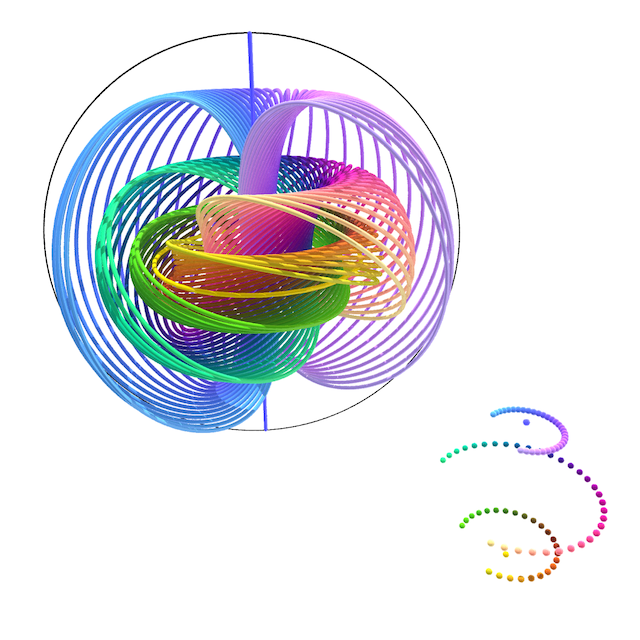
\includegraphics[scale=0.2]{figures/Hopf.png}
        \captionof{figure}{Hopf fibration in stereographic projection, i.e., as a fibration of $\bbR^3$. Each circle is a fiber corresponding to a point on the 2-sphere at the bottom. From \cite{hopf}.}
        \label{Fig.Hopf}
    \end{minipage}
\end{example}

\begin{xca}
    Show that in the Hopf bundle, the preimage of any circle in $\bbS^2$ is a two-torus $\bbT^2$ embedded into $\bbS^3$.
\end{xca}


\begin{defn}[Bundle morphism]\index{Bundle morphism}
    Let $E\overset{\pi}{\to}M$ and $E'\overset{\pi'}{\to}M'$ be two smooth \glspl{fb}. A bundle morphism (a.k.a.\ \emph{bundle map}) between them is a pair of smooth maps $h:E\to E'$ and $\underline{h}:M\to M'$ such that $h$ \emph{covers} $\underline{h}$ in the sense that the following square commutes:
    \[\begin{tikzcd}[every matrix/.append style={name=m},   
    execute at end picture={\draw [<-] ([xshift=-8mm,yshift=1mm]m-2-2.north) arc[start angle=-90,delta angle=270,radius=0.25cm];}]
       E \arrow[r,"h"]\arrow[d,swap,"\pi"]& E'\arrow[d,"\pi'"] \\
       M\arrow[r,swap,"\underline{h}"]& M'
    \end{tikzcd}\]
    We call $\underline{h}$ the \emph{base map}, or the \emph{projection}, of $h$, since it can be uniquely recovered from $h$.\index{Base map}
    This gives rise to the category $\FB^\infty$ of all smooth \glspl{fb}. A full subcategory is the category $\FB^\infty_M$ of all smooth \glspl{fb} over a given base $M$ with $\underline{h}=\id_M$ (note that, in general, there are other bundle morphisms between bundles over $M$ for which $\underline{h}$ is not even a diffeomorphism). Bundle morphisms covering the identity are also called \emph{vertical}.\index{Vertical morphism}
\end{defn}








\section{Structure groups}\label{sec: structure groups}

So far we have only given a purely topological (or geometric in the smooth case) description of \glspl{fb}. The fascinating thing about \glspl{fb}, however, is that the requirement of local triviality gives rise to an alternative \emph{algebraic} description of \glspl{fb}, which will eventually lead us into the realm of cohomology. A similar, but more cumbersome, description appears for general topological fibrations as well. We now characterize smooth \glspl{fb} in terms of their systems of local trivializations and identify their transition maps with certain Lie group actions. Note that everything here easily translates to the category of topological \glspl{fb} as well.


\begin{defn}[Bundle atlas]\label{def G-bundle}\index{Atlas!Bundle}
    Let $E\overset{\pi}{\to}M$ be a smooth \gls{fb} with typical fiber $F$, and let $\{U_\alpha\}_\alpha$ be an open covering of $M$ such that the restrictions $\restr{E}{U_\alpha}$ are trivial. By definition of local triviality, we have some diffeomorphisms $\chi_\alpha: \restr{E}{U_\alpha}\to U_\alpha\times F$, called \emph{local trivializations}. Then:
\begin{enumerate}
    \item The collection $\{(U_\alpha,\chi_\alpha)\}$ is called a \emph{\gls{fb} atlas} for $E\overset{\pi}{\to}M$. Two bundle atlases are \emph{equivalent} if their union is still a bundle atlas. A \emph{bundle structure} on $E$ is an equivalence class of bundle atlases, or, alternatively, a \emph{maximal atlas} given by the union of all atlases belonging to an equivalence class.
    \item For any point $(m,f)\in U_{\alpha\beta}\times F$, the transition maps in this atlas have the form \[\chi_\beta\circ\chi_\alpha^{-1} (m,f)=(m, t_{\beta\alpha}(m,f)),\label{eq transition functions}\]
    where for every fixed $m\in M$, the map $t_{\beta\alpha}(m,\_):F\to F$ is a diffeomorphism. One can think of $t_{\beta\alpha}$ as a function on $U_{\alpha\beta}$ that takes values in the group $\Diff(F)$ of all diffeomorphisms of $F$, so $t_{\beta\alpha}$ becomes a map $t_{\beta\alpha}:U_{\alpha\beta}\to \Diff(F)$.\footnote{As we will see in \S\ref{sec: Diff groups}, the group $\Diff(F)$ can be given the structure of an infinite-dimensional Lie group, modeled on the space $\fX(F)$ of vector fields. Unfortunately $t_{\alpha\beta}$ are not always automatically smooth: they are smooth iff their values are contained in the left coset of the open and closed subgroup $\Diff_c(F)$ of diffeomorphisms with compact support. This is in principle true only for bundles which are ``trivial near fiber-wise infinity'' or have ``discrete structure group near fiberwise infinity'' \cite{Michor}. We shall always assume that this is true.}
    These $\Diff(F)$-valued functions are called \emph{bundle transition functions}. They are also sometimes called \emph{clutching functions}, especially when $M$ is a sphere.\index{Clutching functions}\index{Transition functions} We will usually assume that $\Diff(F)$ acts on the typical fiber from the \emph{left} (one can pass to a right action by acting via $t_{\alpha\beta}^{-1}$ instead).
\end{enumerate}
\end{defn}

\begin{defn}[$G$-structure]
    If the bundle structure of $E$ contains a bundle atlas whose transition functions take values in a Lie subgroup $G<\Diff(F)$,\footnote{We will formalize the concept of Lie subgroups in \S\ref{sec: Lie theory iii}. For now all we need to know is that Lie subgroups are weakly embedded, which means that restricting a smooth map into $\Diff(F)$ whose image lies in $G<\Diff(F)$ in its range produces a smooth map into $G$. In fact, all subgroups of a Lie group are Lie subgroups.} then such an atlas is called a \emph{$G$-atlas} for $E$. Two $G$-atlases are called \emph{$G$-equivalent} if their union is still a $G$-atlas. A $G$-equivalence class of $G$-atlases, or, alternatively, the maximal $G$-atlas equal to their union, is called a \emph{$G$-structure}, denoted $\calG$.\index{$G$-structure} If a $G$-structure is fixed on $E$, we say that $G$ is the \emph{structure group} of the bundle. \index{Structure group} The tuple $(E\overset{\pi}{\to}M,G\acts F,\calG)$ is called a \emph{$G$-bundle}.\index{$G$-bundle}
    
    If $H<G$ is a Lie subgroup and a given $G$-structure on $E$ contains an $H$-atlas, then a choice of an $H$-structure (which is a subset of the given $G$-structure) is called a \emph{reduction of the structure group}, or simply a \emph{bundle reduction}\index{Bundle reduction} from $G$ to $H$.
\end{defn}    

\begin{defn}[Cocycles]
    From the definition \eqref{eq transition functions} it is obvious that the group-valued bundle transition functions satisfy two important conditions:
    \[
    \begin{cases}
    t_{\alpha\alpha}\equiv e, & \text{(identity condition),}\\
    \restr{t_{\alpha\beta}\cdot t_{\beta\gamma}\cdot t_{\gamma\alpha}}{U_{\alpha\beta\gamma}}\equiv e; & \text{(cocycle condition),}
    \end{cases}
    \]
    where the product in $\Diff(F)$ is just the composition of maps. Any collection of such $G$-valued functions $\{t_{\alpha\beta}\}$ associated to an open covering of $M$ is called a \emph{cocycle}\index{Cocycle} on $M$ with structure group $G$.\footnote{More precisely, a cocycle is a certain equivalence class of such collections, which is discussed below.} Note that these two conditions imply $t_{\alpha\beta}t_{\beta\alpha}=e$.
\end{defn}

\begin{rem}\label{rem: faithful action on F 0}
    \begin{enumerate}
        \item One can try writing down higher-order relations on the transition functions, such as $t_{\alpha\beta}t_{\beta\gamma}t_{\gamma\delta}t_{\delta\alpha}=e$, but all of them follow from the identity and the cocycle conditions. On the other hand, replacing the cocycle condition with only $t_{\alpha\beta}t_{\beta\gamma}=e$ would have been insufficient because this does \emph{not} imply the higher-order relations.
        \item $\Diff(F)$ acts on $F$ faithfully by definition, therefore, the induced action of any subgroup $G<\Diff(F)$ is faithful as well. This is why in the following definitions we will assume that the action of the structure group on the model fiber is faithful. We will further elucidate the importance of faithfulness in Remark~\ref{rem: faithfulness of action on F}.
        \item A \gls{fb} $E\to M$ is trivial iff it admits an $\{e\}$-structure. Indeed, if there is a bundle atlas in which all transition functions evaluate to the identity, then all local trivializations agree on the overlaps and hence stitch into a global trivialization. An $\{e\}$-structure is also called an \emph{absolute parallelism}.\index{Parallelism!Absolute}
    \end{enumerate}
\end{rem}


Since the structure group of a bundle acts on its typical fiber $F$, that is, it acts in the local trivializations, it is natural to ask whether this action ``lifts'' to an action on the actual fibers of the bundle itself. Crucially, the answer is no, however, the following restricted concept of a $G$-structure does get naturally translated to the fibers.

\begin{defn}[$G$-fiber]
    Let $F$ be a smooth manifold diffeomorphic to a given manifold $F_0$ and let $G$ be a Lie group acting faithfully from the left on $F_0$, so $G$ can be identified with a Lie subgroup of $\Diff(F_0)$. Two diffeomorphisms $\chi_1,\chi_2:F\to F_0$ are called $G$-equivalent if $\chi_2\circ \chi_1^{-1}\in G$. A $G$-equivalence class $\calG_0$ of such diffeomorphisms, i.e., an orbit of the action of $G$ on $\Diff(F,F_0)$ by compositions $\chi\mapsto g\circ \chi$, is called a \emph{fiber $G$-structure} on $F$.\footnote{This particular terminology is not standard. In common jargon, what is defined here is a $G$-structure on the bundle consisting of one fiber over a single point, $F\overset{\pi}{\to}\ast$.} The tuple $(F,G\acts F_0,\calG_0)$ is called a $G$-fiber modeled on $F_0$. An element of $\calG_0$ is called a \emph{$G$-frame}, or a frame \emph{compatible} with the $G$-structure.\footnote{It would be more appropriate to call the $\chi$ \emph{coframes}, whereas the corresponding frame is $\chi^{-1}$, but we shall ignore this distinction until we focus on affine $G$-structures.} \index{$G$-frame}\index{$G$-structure!Fiber}\index{$G$-fiber}
\end{defn}


\begin{prop}\label{prop G-fibers}
    If $\pi:E\to M$ is a \gls{fb} with structure group $G$ acting on the typical fiber $F$, then each fiber of $E$ naturally carries a fiber $G$-structure and an action of the center $\rmZ(G)$.
\end{prop}
\begin{proof}
    Consider a fiber $E_m=\pi^{-1}(m)$, $m\in M$. The fact that it carries a fiber $G$-structure is obvious because the value of any $G$-valued transition function at a point $m$ is an element of $G$. 
    
    We now show that if $G$ is not abelian, then there is no natural action of $G$ on the fibers, but there is an action of $\rmZ(G)$. By definition of the typical fiber, there is a diffeomorphism $f_\alpha=\restr{\chi_\alpha}{E_m}:E_m\to F$, which is just the restriction of a local trivialization $\chi_\alpha$. By definition of a $G$-structure, there is a smooth (say left) action of $G$ on the typical fiber $F$. Let $f_\beta:E_m\to F$ be the diffeomorphism coming analogously from another compatible local chart. Then $f_\alpha(p)=t^{-1}\cdot f_\beta(p)$ for all $p\in E_m$ for some $t\in G$, and we can compare what the action of an element $g\in G$ translates to in the fiber $E_m$ under these two diffeomorphisms:
    \[f_\alpha^{-1}(g\cdot f_\alpha(p))=f_\beta^{-1}(tgt^{-1} f_\beta(p)).\]
    Since $t$ can range over all of $G$ by varying the charts, these formulas consistently define an action $g\cdot p$ only for $g\in \rmZ(G)$.
\end{proof}

\begin{rem}
    \begin{enumerate}
        \item The intuition behind the definition of $G$-structures is the following. A fiber $G$-structure on $F$ is a choice of a $G$-invariant subset of all diffeomorphisms from $F$ to a ``standard'', or ``model'', space $F_0$, namely an orbit of the action of $G$ on all such diffeomorphisms by compositions. This can be interpreted as $F_0$ having some kind of ``structure'' that is invariant under actions of $G$, and a fiber $G$-structure allows us to transplant this structure to $F$. A $G$-structure on a fiber bundle, then, is a collection of structures on each fiber that, in a sense, vary smoothly with the base point $m\in M$. These structures are defined consistently because all local trivializations belonging to the same $G$-bundle atlas differ from each other by an action of $G$ on $F_0$, hence this additional structure is independent of the local bundle chart. 
        \item Morphisms between bundles with the same structure group are also defined so as to ``respect'' this structure. Thus the smaller the $G$, the more structure the morphisms of this category preserve. We will use this rough idea when introducing vector bundles, orientations, and complex bundles. For example, vector bundles will have group structure $\GL(V)$ for some vector space $V$, and, as we will see, the corresponding fiber $G$-structure is the structure of vector space.
        
        \item There is one extremely special class of $G$-bundles that will be distinguished by the fact that their typical fiber supports \emph{two} commuting actions of $G$, a left one and a right one (because the typical fiber will be $G$ itself). After using one of them up to define the bundle, we will be able to use the above procedure to lift the other one to a global action of $G$ on $E$. These bundles are called \emph{principal}. In \S\ref{sec: free proper actions} we will show that principal $G$-bundles can be defined without reference to local trivializations, and in \S\ref{sec: principal bundles} that will lead us to a chart-free definition of \emph{all} \glspl{fb}.
    \end{enumerate}
\end{rem}
\begin{example}
    A covering space $E\overset{\pi}{\to} M$ is a topological \gls{fb} with a discrete typical fiber $F$. Its structure group, most generally, is the group $G=\Diff(F)=\mathrm{Bij}(F)$ of all permutations of points of the fiber. As we know, there is a natural $\pi_1(M,x_0)$-action on $F=\pi^{-1}(x_0)$, which produces a homomorphism $\lambda:\pi_1(M,x_0)\to G$. Note that there is no natural action of $\pi_1(M,x_0)$ on \emph{other} fibers of $E$ because there is no natural way to choose the isomorphisms between the groups $\pi_1(M,x_0)$ for different choices of the basepoint $x_0$. The image of $\lambda$ is a subgroup of $G$. Since the covering space can be fully reconstructed from this action, $\lambda(\pi_1(M,x_0))$ can be made the structure group of this bundle. 
    
    One case where there is a global action of the structure group on the whole covering space is when it is a $G$-principal covering space. In this case the fiber is $G$ itself and supports a second (right) action of $G$ which survives the \gls{fb} construction.
\end{example}






\section{Fiber morphisms}\label{sec: fiber morphisms}

Now we examine morphisms (and in particular isomorphisms) between bundles with different structures on them. General bundle morphisms are allowed to be arbitrary smooth maps when restricted to a single fiber, so we will need to find a special subclass of bundle morphisms that ``respects'' given structures in some way. Let us first look at the simpler case of a single fiber. Say we have a $G$-fiber $(F,G\acts F_0,\calG_0)$ and a $G'$-fiber $(F',G'\acts F_0',\calG_0')$. Then any map $h:F\to F'$ can be represented by a map $\wh{h}:F_0\to F_0'$ by using any two diffeomorphisms $\chi\in\calG_0\subset \Diff(F,F_0)$ and $\chi'\in\calG_0'\subset \Diff(F',F_0')$ as follows:
\[\wh{h}=\chi'\circ h\circ \chi^{-1}.\label{eq g-fiber f-hat}\]
Different choices of $\chi$ and $\chi'$ are equivalent to replacing $\wh{h}$ in this formula with $g'\circ \wh{h}\circ g^{-1}$ for some $(g,g')\in G\times G'$. Therefore, we notice the importance of the action of the product group $G\times G'$ on the set $C^\infty(F_0,F_0')$ by compositions:
\[G\times G'\acts C^\infty(F_0,F_0'):\quad ((g,g'),\wh{h})\mapsto g'\circ \wh{h}\circ g^{-1}.\label{eq gg' action}\] 
A choice of a class of morphisms $\wt h$ then corresponds to a choice of a set of orbits of this action. For this we either need $F_0$ and $F_0'$ to carry additional structure (vector spaces, metric spaces, etc.) that provides such a choice in a canonical way, or to just specify the choice manually. If want to make these choices consistently across all possible pairs of model spaces $(F_0,F_0')$, this amounts to forming a category. We detail these methods below:
\begin{enumerate}
    \item Let $\calS$ be a subcategory of the category $\mathsf{Man}^\infty$ of smooth manifolds (it need not include neither all objects nor all morphisms). Then if the model spaces $F_0$ and $F_0'$ are objects of $\calS$, we denote
    \[\calS(F_0,F_0')=\mor_\calS(F_0,F_0').\]
    We think of the category $\calS$ as describing ``additional structure'' on the model spaces. We now define morphisms from $(F,G\acts F_0,\calG_0)$ to $(F',G'\acts F_0',\calG_0')$ as maps $h:F\to F'$ which, under some (and therefore, any) diffeomorphisms $\chi\in\calG_0$ and $\chi'\in\calG_0'$, are represented by maps $\wh{h}:F_0\to F_0'$ belonging to $(G\times G')\cdot \calS(F_0,F_0')$.
    
    \item In the situation of item 1, it is also often the case that $G$ and $G'$ \emph{act by automorphisms}, i.e., by elements of $\Aut_\calS(F_0)$ and $\Aut_\calS(F_0')$, respectively. Then 
    \[(G\times G')\cdot \calS(F_0,F_0')=\calS(F_0,F_0').\]
    This situation comes with an extra benefit. Since $G$ preserves the additional structure on $F_0$, this structure can be ``lifted'' via any $\chi\in \calG_0$ so that $F$ itself naturally becomes an object of $\calS$. Thus, in addition to the action of $\rmZ(G)$, the fiber will inherit some additional structure from the $G$-invariant structure on the model fiber. We will soon see how this works explicitly on the example of vector bundles.
    \item The most common setting is a special sub-case of 2, whereby $G$ and $G'$ are \emph{defined} as the groups of automorphisms of $F_0$ and $F_0'$, respectively, so we don't even need to specify them separately:
    \[G=\Aut_\calS(F_0),\quad G'=\Aut_\calS(F_0').\]
    The actions of $G$ and $G'$ in this case are given canonically, and we can proceed as in 1. In particular, this implies that every representative $\wh{h}$ of every \emph{automorphism} (invertible morphism of a $G$-fiber to itself) $h$ is an element of $G$.
\end{enumerate}

\begin{defn}[Category of $\calS$-fibers]\label{def S-fibers}
    Given a $G$-fiber $(\tuple{F,G\acts F_0,\calG_0})$, a $G'$-fiber $(\tuple{F',G'\acts F_0',\calG_0'})$, and a subset $\calS(F_0,F_0')\subset C^\infty(F_0,F_0')$ determined from a category $\calS$ in one of the ways described above, a morphism between them is a smooth map $h: F\to F'$ such that its representative $\wh{h}$ defined by \eqref{eq g-fiber f-hat} using any $\chi\in\calG_0$ and $\chi'\in\calG_0'$ belongs to the orbit of an element of $\calS(F_0,F_0')$ under the action \eqref{eq gg' action} of $G\times G'$ on $C^\infty(F_0,F_0')$. We say that $h$ \emph{is modeled on} an element of $\calS(F,F')$. We call this category $\calS\mathsf{-Man}^\infty$ and its objects $\calS$-fibers. Note that $\calS$ is not enough to define this category -- one also needs to specify groups $G$ and their actions (unless $G=\Aut(F_0)$ as in case 3 above).

    In particular, two $G$-fibers $(F,G\acts F_0,\calG_0)$ and $(F',F\acts F_0,\calG_0')$ with the same structure group $G$ and model space $F_0$ are isomorphic iff there exists a diffeomorphism $h:F\to F'$ such that the map $\calG_0'\to \calG_0$ given by the composition $\chi'\mapsto h^\ast \chi'=\chi'\circ h$ is a bijection. If $G=\Aut_\calS(F_0)$, then this is equivalent to $\wh{h}\in G$ for all representatives \eqref{eq g-fiber f-hat} of $h$.
\end{defn}

Note that the choice of the category $\calS$ for a given type of structure is not unique. In fact, we mostly need this definition to produce a unique notion of \emph{isomorphism} of $\calS$-fibers and later $\calS$-bundles, whereas we won't really care what the rest of the morphisms look like. We now consider a number of important examples of $\calS$-fiber structures.
\begin{example}[Linear $G$-structures]\label{ex linear G-structures}
    \begin{enumerate}
        \item If $\calS=\mathsf{FinVect}_\bbK$ (finite-dimensional $\bbK$-vector spaces), then we get the category of $\mathsf{FinVect}_\bbK$-fibers with linear maps. Here, if the model space is $V$, then we define $G=\Aut_\calS(V)=\GL(V)$. A $G$-structure $\calG_0$ on $F$ is an equivalence class of diffeomorphisms $F\to V$ that differ by an automorphism of $V$. Since $V$ is a vector space, we can use any of these diffeomorphisms $\chi\in\calG_0$ to induce a vector space structure on $F$ itself: for $\lambda_1,\lambda_2\in\bbK$ and $e_1,e_2\in F$ we define the linear combination
        \[\lambda_1e_1+\lambda_2 e_2\coloneqq \chi^{-1}(\lambda_1\chi(e_1)+\lambda_2\chi(e_2)).\]
        This is well-defined because different $\chi$'s differ by a linear automorphism of $V$. In particular, this defines an action of scalar matrices $\lambda I$, $\lambda\in\bbK$, on $F$, which coincides with the induced natural action of the center $\rmZ(G)$. Note that $\GL(V)$ has no natural action on $F$ because there is no natural isomorphism between $F$ and $V$! Thus the category $\calS\mathsf{-Fib}$ is isomorphic to $\calS$ itself.

        In fact, one can replace the category $\mathsf{FinVect}_\bbK$ with its skeleton $\mathsf{Sk}(\mathsf{FinVect}_\bbK)$, whose objects are \emph{standard} spaces $\bbK^n$, $n=0,1,\ldots$, and the only nontrivial morphisms are inclusions-as or projections-onto the first $n$ components. Indeed, every linear map between vector spaces is represented by one of these standard maps in some appropriately chosen bases of the source and target spaces. In this case an element of $\calG_0$, i.e., a \emph{frame}, determines a basis on $F$ and outputs the components of vectors in that basis.
        
        \item In general, if structure groups $G$ are defined as the automorphism groups $\Aut(F_0)$, then the resulting category $\calS\mathsf{-Fib}$ is equivalent to $\calS$ itself. This allows one to define many classical structures on vector spaces in terms of a countable set of ``standard'' ones. This shows the importance of allowing $G$ to not necessarily act by automorphisms. We proceed in this manner in the next several examples.
        
        \item If $\bbK=\bbR,\bbC,\bbH$, then we can let $\calS$ be the category of finite-dimensional vector spaces with a $\bbK$-valued inner product, or its skeleton consisting of spaces $\bbK^n$ with the standard dot product $\sum_{i=1}^n \wb{x}_i y_i$. For each model space $\bbK^n$ we also take its isometry group $G$, which is $\Or_n,\U_n$, or $\Sp_n$, respectively. Then $\calS$-fibers are vector spaces $F$ with a $G$-structure which allows us to lift the inner product onto $F$. There is a bijective correspondence between $G$-structures and inner products on $F$, so  $\calS\mathsf{-Fib}$ is exactly the category of vector spaces with an inner product and all linear maps. $G$-frames in this context are just orthonormal bases. We can also replace $\calS$ with the category of vector spaces $V$ with an inner product and linear morphisms whose operator norm is at most $1$ (this forces isomorphisms to be isometries), and letting $G=\Aut_\calS(V)$. Then $\calS\mathsf{-Fib}$ has the same objects but fewer morphisms.

        \item If we let $\calS=\mathsf{FinVect}_\bbK$ but redefine the structure group $G$ of a model space $V$ as $G=\GL^+(V)$, i.e., orientation-preserving automorphisms, then $\calS$-fibers are oriented vector spaces with linear maps between them. 

        \item If $\calS$ is again the category of standard real vector spaces $\bbR^n$, $n=0,1,\ldots$, and the structure group of $\bbR^n$ is $\SL_n(\bbR)$, then $\calS$-fibers are vector spaces with a volume form (a totally antisymmetric multilinear form of maximum rank) with linear maps between them. Alternatively we can let $\calS$ consist of $\bbR^n$'s with the standard volume form $\mathsf{v}_n$ and linear maps $f:\bbK^n\to \bbK^m$ such that $f^\ast \mathsf{v}_m=\lambda \mathsf{v}_n$ with $\lambda\in (-1,1]$ (this forces automorphisms to have determinant $1$), and define $G=\Aut_\calS(\bbR^n)\cong \SL_n(\bbR)$. Note that a volume form induces an orientation because $\SL_n(\bbR)\subset \GL_n^+(\bbR)$.

        \item Taking standard model spaces $\bbK^n$ with $G$ defined as the group that leaves the subspace $\bbK^p$ spanned by the first $p$ standard basis vectors, and linear maps that map the first $p$ directions of one space to the first $p$ directions of the other (not necessarily surjectively), we get the category $\calS\mathsf{-Fib}$ of vector spaces with ``$p$-directions''. It is isomorphic to the category of pairs $(V,W)$ where $W$ is a $p$-dimensional subspace of $V$, and morphisms are required to be maps of pairs (i.e., $W$ is mapped inside $W'$). Note that morphisms between standard spaces $\bbR^n\to \bbR^m$ are represented by matrices with the top right $p\times(n-p)$ block filled with zeroes (unless $p>m$, in which case it's just the right $m\times (n-p)$ block).

        \item Consider all free actions of the group $G=\GL_n(\bbZ)$ on $n$-dimensional vector spaces $V$. This means that $G$ is the group of linear automorphisms of $V$ that preserve some rank-$n$ lattice $\varLambda$ spanning $V$ (i.e., $\varLambda=\bbZ v_1+\cdots +\bbZ v_n$ for some basis $v_1,\ldots,v_n$). Then $\calS\mathsf{-Fib}$ is the category of vector spaces with an \emph{integral affine structure}. It is isomorphic to the category of pairs $(V,\varLambda)$ and linear maps mapping lattice to lattice.

        \item $\calS$ be the category of even-dimensional real vector spaces $V$ with a linear isomorphism $\sfJ:V\to V$ such that $\sfJ^2=-\id_V$ (called a \emph{complex structure})\index{Complex structure} and linear maps $h:(V,\sfJ)\to(V',\sfJ')$ such that $h\circ \sfJ=\sfJ'\circ h$ (called \emph{complex linear w.r.t.\ $\sfJ$}). Each $\sfJ$ defines a structure of a $\bbC$-vector space on $V$ via $\rmi v\coloneqq\sfJ(v)$. Then $G=\Aut_\calS(V)$ consists of matrices $A\in\GL(V)$ such that $\sfJ A=A\sfJ$ and is isomorphic to $\GL_n(\bbC)$ (exercise). This group is denoted $\GL(V,\sfJ)$ or simply $\GL_\bbC(V)$. The category $\calS\mathsf{-Fib}$ is isomorphic to $\calS$ itself and is the category of complex structures on real vector spaces with complex-linear maps between them. $\calS$ can also be replaced with its skeleton, which consists of standard complex structures on $\bbR^{2n}$:
        \[\rmJ_{n}=\begin{bmatrix}
            0&-\rmI_n\\
            \rmI_n&0
        \end{bmatrix}\]
        And linear maps $f:\bbR^{2n}\to \bbR^{2m}$ that satisfy $\rmJ_{m}\circ f=f\circ \rmJ_{n}$. In the case $m=n$ such maps are called holomorphic and their matrices have the form 
        \[M=\begin{bmatrix}
            A&B\\
            -B&A
        \end{bmatrix},\label{eq complex matrices}\]
        which can be identified with $A+\rmi B\in \Mat_n(\bbC)$.
        Note that each complex structure also induces an orientation because matrices $A\in \GL_n(\bbC)\subset \GL_{2n}(\bbR)$ have positive determinant over $\bbR$, namely $\det M=|\det(A+\rmi B)|^2>0$.

        \item Consider standard spaces $\bbR^{2n}$ with standard symplectic forms, i.e., antisymmetric nondegenerate bilinear forms $\omega_n:\bbR^{2n}\times \bbR^{2n}\to \bbR$ whose matrix in the standard basis is $\rmJ_{n}$. Let morphisms be all linear maps and let $G=\Sp_{2n}(\bbR)$ be the group of symplectic matrices, i.e., matrices $A\in\GL_{2n}(\bbR)$ such that $A^T\rmJ_{n}A=\rmJ_{n}$. Then $\calS$-fibers are symplectic vector spaces $(V,\omega)$ with all linear maps between them. This can be reduced to just the category of \emph{symplectomorphisms}, i.e., isomorphisms that preserve the symplectic structure.
    \end{enumerate}
\end{example}


\begin{example}[Hermitian structures]\label{ex hermitian structures}
    A Hermitian structure on a complex vector space $V_\bbC$ is just a symmetric sesquilinear form $\sfh:V_\bbC\times V_\bbC\to \bbC$ as introduced in the preceding example, i.e.,
    \[\sfh(v,w)=\widebar{{\sfh}(w,v)},\quad v,w\in V_\bbC,\]
    and $\sfh(v,v)\geq 0$ for all $v\in V_\bbC$ and vanishes iff $v=0$.
    
    An $n$-dimensional complex vector space is naturally isomorphic to a $2n$-dimensional real vector space with a complex structure $V_\bbC\cong (V,\sfJ)$ (defined by $\sfJ(v)\coloneqq \rmi v$), also denoted $V_\sfJ$. Then $\sfh$ can be reinterpreted as a complex-valued $\bbR$-bilinear form on $V_\sfJ$ which in addition satisfies
    \[\sfh(v,\sfJ w)=-\sfh(\sfJ v,w)=\rmi\sfh(v,w),\quad v,w\in V_\sfJ,\]
    and such that $\sfh(v,v)$ is a norm. This also implies that
    \[\sfh(\sfJ v,\sfJ w)=\sfh(v,w).\]
    We can decompose $\sfh$ into its real and imaginary parts, which we suggestively call $\sfg$ and $\omega$:
    \[\sfh(v,w)=\Re \sfh(v,w)+\rmi\Im\sfh(v,w)=\sfg(v,w)+\rmi \omega(v,w).\]
    We have
    \[\sfg(v,w)=\Re \sfh(v,w)=\Re \sfh(w,v)=\sfg(w,v),\]
    and $\sfg(v,v)=\sfh(v,v)$, therefore, $\sfg$ is a nondegenerate symmetric bilinear form that defines an inner product on $V_\sfJ$.
    Furthermore, the sesquilinear condition implies that 
    $\omega(v,w)=\frac12 (\rmi\sfh(w,v)-\rmi\sfh(v,w))=\frac12 (\sfh(w,\sfJ v)-\sfh(v,\sfJ w))$
    is a real antisymmetric bilinear form. 
    Moreover,
    \[\omega(v,\sfJ w)=\frac12 (\sfh(\sfJ w,\sfJ v)+\sfh(v,w))=\frac12 (\sfh(w,v)+\sfh(v,w))=\Re \sfh(v,w)=\sfg(v,w),\]
    therefore, $\omega$ is nondegenerate as well, and hence determines a symplectic structure on $V_\sfJ$. 

    Crucially, fixing a complex structure $\sfJ$, the above formulas relating any two of the three objects $\sfh,\sfg,\omega$ uniquely determine the third. We thus have natural isomorphisms between the following three pairs of structures:
    \begin{enumerate}
        \item Hermitian structures $(\sfJ,\sfh)$ on $V$.
        \item Pairs $(\sfJ,\sfg)$ of a complex structure $\sfJ$ and a metric $\sfg$ that are compatible in the sense that
        \[\sfg(\sfJ v,\sfJ w)=\sfg(v,w),\quad \text{or}\quad \sfg(\sfJ v,w)=-\sfg(v,\sfJ w),\quad v,w\in V.\]
        This compatibility condition is equivalent to the bilinear form $\omega_\sfJ(v,w)=\sfg(\sfJ v,w)$ being a symplectic form, also called the \emph{fundamental form}.
        \item Pairs $(\sfJ,\omega)$ of a complex structure $\sfJ$ and a symplectic structure $\omega$ that are compatible in the sense that
        \[\omega(\sfJ v,\sfJ w)=\omega(v,w),\quad \text{or}\quad \omega(\sfJ v,w)=-\omega(v,\sfJ w),\quad v,w\in V,\]
        and in addition that the resulting form $\sfg_\sfJ(v,w)=\omega(v,\sfJ w)$, which is symmetric because of compatibility, is positive definite (in this case we say that $J$ \emph{tames} $\omega$). These conditions are equivalent to the bilinear form $\sfg_\sfJ$ being a real inner product.
        \item Pairs $(\sfg,\omega)$ of a positive definite metric $\sfg$ and a symplectic form $\omega$. By non-degeneracy of $\sfg$, there exists a unique operator $\sfJ$ such that $\omega(v,w)=\sfg(v,\sfJ w)$, and it follows that $\sfJ$ is a complex structure compatible with both $\sfg$ and $\omega$.
    \end{enumerate}
    Thus the group of isometries of $\sfh$, $\U(V,\sfh)$, coincides with the following double intersections of groups $\Sp(V,\omega)$ (automorphisms preserving $\omega$), $\GL(V_\bbC)$ (automorphisms preserving $\sfJ$), and $\Or(V,\sfg)$ (automorphisms preserving $\sfg$):
    \[\U(V,\sfh)=\Sp(V,\omega)\cap \GL(V_\bbC)=\Or(V,\sfg)\cap \GL(V_\bbC)=\Or(V,\sfg)\cap \Sp(V,\omega).\]
    In particular, for standard model spaces $(\bbR^{2n},\rmJ_{n})$ we get the \emph{``2 out of 3 property of unitary groups''}:
    \[\U_n=\Sp_n(\bbR)\cap \GL_n(\bbC)=\Or_{2n}\cap \GL_n(\bbC)=\Or_{2n}\cap \Sp_n(\bbR),\]
    which is also obvious from the fact that any two of the defining equations $A^T\sfJ A=\sfJ$, $A^{-1}\sfJ A= \sfJ$, $A^TA=\rmI$, imply the third.
    Here, $\GL_n(\bbC)$ is included in $\GL_{2n}(\bbR)$ as the set of invertible matrices of the form \eqref{eq complex matrices} identified with $A+\rmi B\in \GL_n(\bbC)$.
    
    The triple $(\sfJ,\sfg,\omega)$ consisting of compatible complex, metric, and symplectic structures on $V$ can be called a \emph{linear K\"ahler structure}.\index{K\"ahler structure} As we have seen, the set of K\"ahler structure is bijective with the set of Hermitian structures, which is why in the linear case the term K\"ahler structure is redundant.
\end{example}

\begin{xca}
    \begin{enumerate}
        \item Show that the space of metrics on a vector space is convex, i.e., for any two metrics $\sfg_1$ and $\sfg_2$, all bilinear forms $t\sfg_1+(1-t)\sfg_2$, $t\in[0,1]$, are also metrics. Hence it is contractible.
        \item Show that the space of Hermitian forms $\sfh$ is also convex and hence contractible.
        \item Show that the set $\calJ(V,\omega)\subset \GL(V)$ of complex structures compatible with a given symplectic form $\omega$ (but not necessarily taming it) is contractible. See \cite[Prop.~7.5.7]{RS1}.
    \end{enumerate}
\end{xca}







\section{Bundle morphisms}\label{sec: bundle morphisms}

Now we extend our definition of morphisms to arbitrary \glspl{fb}. Consider a morphism $h:E\to E'$ between two arbitrary bundles $E\overset{\pi}{\to}M$ and $E'\overset{\pi'}{\to}M'$ with potentially differing structure groups $G$ and $G'$. Pick local trivializations $\{(U_\alpha,\chi_\alpha)\}_{\alpha\in A}$, $\{(U_a',\chi_a')\}_{a\in A'}$ on the two bundles with corresponding cocycles $\{t_{\alpha\beta}\}$ and $\{t_{ab}'\}$ and denote $U_{\alpha a}=U_\alpha\cap \underline{h}^{-1}(U_a')$. Then the bundle morphism is locally represented by maps
$\wh{h}_{\alpha a}:U_{\alpha a}\times F\to F'$ as follows: 
\[\boxed{h\left(\chi_\alpha^{-1}(m,f)\right)=\chi_a^{\prime-1}\left(\underline{h}(m),\wh{h}_{\alpha a}(m,f)\right).}\label{eq def of hab}\]
By transforming to other local charts $\chi_\beta$ and $\chi_b'$ via formula \eqref{eq transition functions} we have
\[h\left(\chi_\beta^{-1}(m,t_{\beta\alpha}(m)\cdot f)\right)=\chi_b^{\prime-1}\left(\underline{h}(m),t_{ba}'(\underline{h}(m))\cdot\wh{h}_{\alpha a}(m,f)\right).\]
On the other hand, \eqref{eq def of hab} written for $\wh{h}_{\beta b}$ implies
\[h\left(\chi_\beta^{-1}(m,t_{\beta\alpha}(m)\cdot f)\right)=\chi_b^{\prime-1}\left(\underline{h}(m),\wh{h}_{\beta b}\left(m,t_{\beta\alpha}(m)\cdot f\right)\right).\]
By comparing the right hand sides of the last two formulas and using the fact that $\chi_b'$ is a fiberwise diffeomorphism, we conclude that
\[\boxed{\wh{h}_{\beta b}\left(m,t_{\beta\alpha}(m)\cdot f\right)=t_{ba}'(\underline{h}(m))\cdot \wh{h}_{\alpha a}(m,f).}\label{eq transformation of hab}.\]
This is a complicated condition on the collection of maps $\{\wh{h}_{\alpha a}\}$ with respect two different cocycles. Despite this condition these maps can still look like completely arbitrary smooth maps when restricted to a single fiber. However, in many cases we would like to consider only those bundle morphisms which, in some sense, respect the given group structures. To this end, consider the set of smooth maps $C^\infty(F,F')$ (which is an infinite-dimensional smooth manifold) and the left action of $G\times G'$ on it by compositions:
\[(G\times G')\acts C^\infty(F,F'):\quad ((g,g'),\varphi)\mapsto g'\circ \varphi\circ g^{-1}.\]
Then every $\hat{h}_{\alpha a}:U_{\alpha a}\times F\to F'$ can be used to define a fiberwise $G\times G'$-equivariant map
\begin{gather}
    \varPhi_{\alpha a}: U_{\alpha a}\times (G\times G')\to C^\infty(F,F'),\\
    (m,(g,g'))\mapsto \left(f\mapsto g'\cdot \hat{h}_{\alpha a}\left(m,g^{-1}\cdot f\right)\right).\label{def Phiab}
\end{gather}
It is easy to see that this map is $G\times G'$-equivariant (with $G\times G'$ acting on itself from the left). Moreover, every fiberwise $G\times G'$-equivariant map arises this way ($\hat{h}_{\alpha a}$ can be recovered by substituting $g=g'=e$), although the correspondence of course is not bijective.\footnote{Note how the fact that $\varPhi_{\alpha a}$ are defined on sets of the form $U_{\alpha a}\times (G\times G')$ hints that they themselves represent a function defined globally on some \gls{fb} with typical fiber $G\times G'$. We will return to this in our discussion of principal bundles.} The transformation rule \eqref{eq transformation of hab} now becomes
\[\boxed{\varPhi_{\beta b}(m,g,g')=\varPhi_{\alpha a}\left(m,gt_{\beta\alpha}(m),g't_{ba}'(\underline{h}(m))\right).}\label{eq transformation of Phiab}\]
We would like to put some restriction on the values of these maps in $C^\infty(F,F')$ that produces a well-defined class of bundle morphisms $h$ which can be interpreted as ``respecting'' the given $G$- and $G'$-structures. This can be easily done by analogy with how we interpreted the structure of a $G$-fiber:
\begin{gather}
    \text{All maps }\{\varPhi_{\alpha a}\}_{\alpha\in A,a\in A'}\text{, at fixed }m\text{, should be required to take values}\\
    \text{in a single orbit of the }G\times G'\text{-action on }C^\infty(F,F').
\end{gather}
This is a well-defined constraint because, due to the equivariance of $\varPhi_{\alpha a}$, the transformation law \eqref{eq transformation of Phiab} implies that the fiber above $m$ gets mapped to the same orbit regardless of the values of the indices $\alpha,a$.

\begin{defn}[Category ${\calS \mFB}^\infty$]\label{def S-bundle}
    Let the objects of the category $\calS\mFB^\infty$, called $\calS$-bundles, be all possible structured bundles $(E\overset{\pi}{\to}M,G\acts F,\calG)$ with model fibers $F\in\ob(\calS)$ and with sets of maps $\calS(F,F')\subset C^\infty(F,F')$ determined from a category $\calS$. Morphisms from such a bundle to another one, $(E'\overset{\pi'}{\to}M',G'\acts F',\calG')$, are bundle morphisms $h:E\to E'$ such that $\calG$ and $\calG'$ contain some $G$- and $G'$-atlas, respectively, in which $h$ is represented by a collection of $G\times G'$-equivariant maps $\{\varPhi_{\alpha a}\}$ as above which satisfy the compatibility condition \eqref{eq transformation of Phiab} and which, for each fixed $m\in M$, take values in the orbit of a single element of $\calS(F,F')$ under the action of $G\times G'$ on the set $C^\infty(F,F')$. We say that $h_m\coloneqq \restr{h}{E_m}$ \emph{is modeled on} an element of $\calS(F,F')$.

    In addition, ${\calS\mFB}_M^\infty$ is the subcategory of structured bundles over the fixed base manifold $M$ with morphisms covering the identity in $M$, i.e., we assume $h=\id_M$.
\end{defn}

There are a number of other subcategories one may define by additionally either fixing the fiber, the structure group, or both. The most important subcategory for us will be the following.

\begin{defn}[Category $\FB^\sigma$]\label{def FB^sigma}
    The category $\FB^\sigma$ consists of so called $(G,\sigma)$-bundles with a fixed structure group $G$, typical fiber $F$, and faithful action $\sigma:G\times F\to F$. The morphisms are required to be such that their local representatives lie in the orbit of the identity map on $F$. That is, locally morphisms are represented simply by actions of elements of $G$ on $F$.
\end{defn}


\begin{example}
    Consider the cylinder $E=\bbS^1\times\bbR $ as a line bundle over the circle. We can trivialize it with all transition functions being the identity. In the category of all line bundles (with structure group $\Diff(\bbR )$) there is a bundle map $E\to E$ that maps $(p,x)\mapsto (p,-x)$. However, in the category of bundles with the trivial structure group $G=\{e\}$ (i.e., the category of trivial bundles) this is not an allowed bundle map because it does not act trivially on the fiber.
\end{example}


\begin{defn}[Bundle construction]\label{def bundle construction}
    \Glspl{fb} can be alternatively defined by specifying the base manifold $M$, the typical fiber $F$, the structure group $G$ acting on the fiber via a \emph{faithful}\footnote{The importance of faithfulness will be explained in Remark~\ref{rem: faithfulness of action on F}.} smooth left action which can be viewed as an injective homomorphism of Lie groups $\varPhi:G\to \Diff(F)$ (i.e., we will write $g\cdot f=\varPhi(g)(f)=\varPhi_g(p)$ for $g\in G, f\in F$), a countable open covering $\{U_\alpha\}$ of $M$, and a cocycle  $t_{\beta\alpha}\in C^\infty (U_{\alpha\beta}, G)$. Namely, we can define $E$ as a topological space as the quotient $E\coloneqq \bigslant{(\bigsqcup_\alpha U_\alpha \times F)}{\sim}$, where $(m_1,f_1)\sim(m_2,f_2)$ iff $m_1=m_2=m$ and $f_1=t_{\beta\alpha}(m,f_2)$ for some $\alpha,\beta$, and the projection $\pi$ is defined as the descendent of the projections onto the fist component in each summand.\footnote{In categorical terms, this is literally the cofibered product (pushout) of the sets $U_\alpha \times F$ with pairs of maps $\restr{\chi_\alpha^{-1}}{U_{\alpha\beta}\times F}$ and $\restr{\chi_\beta^{-1}}{U_{\alpha\beta}\times F}$. For instance, if there were only two sets $U_1,U_2$, we would have $E=(U_1\times F)\sqcup_Z (U_2\times F)$, where $Z=U_{12}\times F$ and we have two morphisms $\restr{\chi_i^{-1}}{U_{12}\times F}:Z\to U_i\times F$ that are used in the definition of the pushout.}
    Then $E$ has a unique smooth structure that makes $\pi$ a smooth submersion (see \cite[Lem.~10.6]{Lee} for the case of vector bundles, which is easily generalized to all \glspl{fb}).\footnote{Essentially we can take an atlas $\{F_\alpha,\psi_\alpha\}$ of $F$ and an atlas $\varphi_\alpha$ of $M$ (\gls{wlog} subordinate to the covering $\{U_\alpha\}$) to construct a smooth atlas $\{(U_\alpha\times F_\beta,\varphi_\alpha\times\psi_\beta)\}$ of $E$.} This construction is called the \emph{clutching construction} of a \gls{fb}.
\end{defn}


The fact that any $(G,\sigma)$-bundle over $M$ can be uniquely reconstructed from a $G$-valued cocycle on $M$ means that this category doesn't really depend on the fiber $F$ and the action $\sigma$ very much. Namely, for any other faithful $G$-action $\sigma':G\times F'\to F'$ there is an equivalence of categories
\[C_{\sigma',\sigma}:\FB^\sigma\to \FB^{\sigma'}.\label{eq equivalence of bundle categories}\]
The functors going in either direction take a bundle, choose a cocycle for it, and then construct the other bundle using the same cocycle via the other action. Faithfulness of the actions is clearly necessary for this to be an equivalence of categories because only then are the cocycles uniquely defined. The key insight flowing from this equivalence is that, to study arbitrary \glspl{fb}, it will suffice to pick one particular kind of typical fibers and group actions on them which makes computations easy. This computationally convenient class of bundles turns out to be the class of \emph{principal bundles}, where the typical fiber coincides with the structure group. We discuss them in the examples below.



\begin{example}[Linear $G$-structures on manifolds]
    \begin{enumerate}
        \item Regardless of $\calS$, if $G=\{e\}$, then an $\{e\}$-structure is equivalent to a global trivialization of the bundle. In the case of vector bundles, this is called an \emph{absolute parallelism}.\index{Parallelism!Absolute}
        \item $\calS=\mathsf{FinVect}_\bbR$, and the structure group of each vector space $F$ is $\GL(V)$, then $\calS$-bundles are just vector bundles. Each fiber is naturally an $\calS$-fiber, i.e., a vector space, and vector bundle morphisms are exactly fiberwise linear bundle morphisms.
        \item A $\GL_k^+$-structure on a vector bundle of rank $k$ is called an orientation because it selects an orientation on every fiber in a continuous fashion. A vector bundle that admits such a structure is called \emph{orientable}.\index{Orientable vector bundle}
        \item An $\Or_k$-structure on a vector bundle $E$ of rank $k$ is equivalent to a smooth choice of metrics $\sfg_m$ on each fiber $E_m$. In \S\ref{sec: Riemannian mfds} we will see that every real manifold admits such a choice, called a \emph{Riemannian structure}, so every vector bundle admits a (non-unique) reduction of the structure group to an orthogonal group. $\Or_k$-bundles are known as \emph{Riemannian bundles}. This fact is equivalent to the statement that $\GL_k(\bbR)$ deformation retracts onto $\Or_n$. In addition, if the bundle is orientable, the structure group can be reduced to $\SO_n$.
        \item A $\GL_k(\bbC)$-structure on a real vector bundle $E$ of rank $2k$ is equivalent to a smooth choice of complex structures $\sfJ_m$ on each fiber $E_m$. Such bundles are called \emph{complex vector bundles} of rank $k$. Every complex vector bundle is oriented.
        \item A $\Sp_{2k}(\bbR)$-structure on a (real) vector bundle $E$ of rank $2k$ is equivalent to a smooth choice of symplectic forms $\omega_m$ on each fiber $E_m$. If such a choice exists, we get a \emph{symplectic vector bundle}.
        \item A $\U_k(\bbR)$-structure on a rank $k$ complex vector bundle is a smooth choice of a Hermitian inner product on each fiber. As we will see, every complex vector bundle admits such a choice, thus any $\GL_k(\bbC)$-structure can be reduced to a $\U_k$-structure. Note that a further reduction to $\SU_k$ is not always possible, and its existence doesn't have a standard name (we will later see that it is equivalent to the triviality of the determinant line bundle $\det E$, or to the vanishing of the first Chern class, $c_1(E)=0$).
    \end{enumerate}
    Note that every one of these structures, just like in the linear case, defines a canonical choice of frames (bases) in each fiber, and via local trivializations they can be chosen smoothly over an open subset of the base. 
\end{example}

\begin{example}[Non-vector $G$-bundles]\label{ex non-vector G-bundles}
    \begin{enumerate}
        \item If $\calS=\mathsf{LieGr}$ with the structure group acting on each Lie group $G$ being its automorphism group $\Aut(G)$, then $\calS$-bundles are called \emph{group bundles}.\index{Group bundle} Since automorphisms preserve the identity and the rest of the group structure, each fiber of a group bundle carries a natural Lie group structure. In particular, each group bundle has one canonical \emph{identity section} $o:M\to E$ whose value in each fiber is the identity element of that fiber.\index{Identity section} This makes group bundles a natural generalization of \glspl{vb}. 
        
        \item If $\calS=\mathsf{LieGr}$ but with the structure group of a Lie group $G$ being $G$ itself acting by left translations, then we get what are called \emph{principal bundles} and they are so important that we shall put off a detailed discussion of them until \S\ref{sec: principal bundles}. For now we only note the crucial difference between group and principal bundles: the fibers of a principal $G$-bundle, despite being diffeomorphic to $G$, are not Lie groups since left translations don't preserve the identity element.\index{Principal fiber bundle} This is another important example where the group action on the typical fiber falls outside of the set of morphisms allowed by $\calS$.
    \end{enumerate}
\end{example}

The following theorem is one of the most important theorems for the applications of \gls{fb} theory, for example in complex analytic problems of differential equations (where it is known as the Riemann-Hilbert factorization problem).

\begin{thm}\label{bundle isomorphism thm}
Two $G$-bundles $E$ and $E'$ over $M$ are isomorphic iff there exists a covering $\{U_\alpha \}$ of $M$, two corresponding cocycles $\{t_{\alpha\beta}\}$ and $\{t_{\alpha\beta}'\}$, and a set of $G$-valued functions $\lambda_\alpha:U_\alpha\to G$ such that $t_{\alpha\beta}'(p)\equiv \lambda_\alpha (p) t_{\alpha\beta}(p) \lambda_\beta^{-1}(p)$ for all $p\in U_{\alpha\beta}$. In particular, a bundle is trivial iff its transition functions can be factorized as $t_{\alpha\beta}=\lambda_\alpha \lambda_\beta^{-1}$.
\end{thm}
\begin{proof}
Given two bundle atlases over $M$, we can always take all possible pairwise intersections of the sets of the two covers of $M$ to refine the atlases so that they are defined over the same covering of $M$. \gls{wlog}, any isomorphism of bundles over the same base can be assumed be identity on the base itself (e.g. because if the horizontal part of the isomorphism is some diffeomorphism $f:M\to M$, we can replace one of the bundles by the isomorphic pullback bundle along $f$, see Definition~\ref{Pullback bundle}). Then from \eqref{eq transformation of hab} we see that any bundle isomorphism gives rise to the $\lambda_\alpha$'s, and vice versa, $\lambda_\alpha$'s completely describe the bundle isomorphism. 
\end{proof}
\begin{defn}[Equivalent cocycles]
    Two $G$-valued cocycles on $M$ that are related (after being brought over to a common set of charts $\{U_\alpha\}$) by the above formulas for some collection of maps $\lambda_\alpha:U_\alpha\to G$ are called \emph{$G$-equivalent}. The equivalence class $[\{t_{\beta\alpha}\}]$ itself is also called a cocycle.
\end{defn}
\begin{cor}
    Given a manifold $M$ and a faithful smooth action $G\overset{\sigma}{\acts} F$, there is a bijective correspondence between isomorphism classes of $(G,\sigma)$-bundles over $M$ and ($G$-equivalence classes of) $G$-valued cocycles on $M$.
\end{cor}
This correspondence can actually be restated as an equivalence of the category $\FB^\sigma$ and a certain category of cocycles, see \cite{Vakar}.

\begin{rem}\label{rem: faithfulness of action on F}
    Faithfulness of the action is crucial here. As we noted in Remark~\ref{rem: faithful action on F 0}, any structure group whose action is induced from the action of $\Diff(F)$ acts on $F$ faithfully. We can see the importance of this property when reconstructing a bundle from a cocycle acting on a model fiber. If, for example, $F$ is a single point, then every group action on $F$ is trivial and there is only one \gls{fb} over $M$ with fiber $F$ regardless of the structure group $G$, whereas there are still many non-equivalent $G$-valued cocycles on $M$. Therefore, faithfulness is needed so that the cocycle is well-defined in this sense. In the future we will run into important situations where, for instance, $F$ is a finite-dimensional vector space with an action of a nonlinear group $G$ (namely a spin group), so that this action cannot be faithful, and thus the correspondence with classes of cocycles will not be one-to-one.
\end{rem}






\section{Flat bundles}

Now let us try to use this transformation rule for transition functions to ``simplify'' the cocycle and see how far we can go. If we have two charts with a transition function $t_{\alpha\beta}$, then we always find a pair of functions $\lambda_\alpha,\lambda_\beta$ on those charts such that $\lambda_\alpha t_{\alpha\beta}\lambda_\beta^{-1}$ is constant, in fact equal to identity: just pick $\lambda_\alpha=e$ and let $\lambda_\beta$ be an arbitrary smooth extension of $t_{\alpha\beta}$ from $U_{\alpha\beta}$ to all of $U_\beta$. We can try to keep expanding this procedure to more and more charts, but there is no guarantee that we will be able to make all transition functions constant. Thus we single out the following important class of bundles.

\begin{defn}[Flat $G$-structure]\index{Flat!fiber bundle}\index{Flat!$G$-structure}\label{def flat G-bundle}
	A $G$-structure on a \gls{fb} is called \emph{flat} if it contains a bundle atlas with constant (or locally constant) transition functions. Alternatively, a $G$-structure is flat if structure group $G$ can be reduced to a subgroup with a \emph{totally disconnected} topology (one where all connected subsets are one-point sets, e.g., the discrete topology; then the transition functions are forced to be constant by continuity). If the default $\Diff(F)$-structure is flat, then the bundle itself is called flat.
\end{defn}
\begin{rem}
    Note that the flatness of the bundle (w.r.t.\ the default $\Diff(F)$-structure) does not imply that all other $G$-structures on it are flat.
\end{rem}


\begin{example}[Line bundles above $\bbS^1$]\label{line bundles over S1}
    We can use the idea of a bundle atlas and Theorem~\ref{bundle isomorphism thm} to classify all line bundles above the circle up to isomorphisms. It suffices to pick one covering of the circle, so we will pick a covering by the three circular arcs $U_1=(\epsilon,4\pi/3-\epsilon)$, $U_2=(2\pi/3+\epsilon,2\pi-\epsilon)$, and $U_3=(4\pi/3+\epsilon,8\pi/3-\epsilon)$. The transition functions in a line bundle take values in the group $G$ of diffeomorphisms of $\bbR $. Each such diffeomorphism is a smooth function $f:\bbR \to\bbR $ such that $f'$ is never zero. Now, clearly $G$ consists of two path-connected components, one of diffeomorphisms that preserve the orientation, i.e., $f'(x)>0$ for all $x$, and others that reverse it, $f'(x)<0$. We say that these diffeomorphisms have one of two possible \emph{parities}. Let $g_+(x)=\id_{\bbR }(x)=x$ and $g_-(x)=-x$, so that $g_+$ is the identity element of $\Diff(\bbR )$ and $g_-$ is an orientation-reversing involution.

    There are three transition functions, $t_{12}$, $t_{23}$, and $t_{31}$. Any three $G$-valued functions $\lambda_1,\lambda_2,\lambda_3$ provide an isomorphic line bundle. Choose $\lambda_1\equiv g_+$. Furthermore, $t_{12}:U_{12}\to G$ can be extended to a continuous function $\lambda_2: U_2\to G$, $\restr{\lambda_2}{U_{12}}=t_{12}$. Then $t_{12}'=\lambda_1 t_{12}\lambda_2^{-1}\equiv g_+$. By continuity, all values of $\lambda_2$ have the same parity.  Now, we let $\lambda_3$ be a continuous extension to $U_3$ of the function $\lambda_2 t_{23}:U_{23}\to G$. Then $t_{23}'=\lambda_2 t_{23} \lambda_3^{-1}\equiv g_+$. Finally, $t_{31}'=\lambda_3 t_{31} \lambda_1=\lambda_3 t_{31}$.  The parity of the values of $t_{31}'$ by construction is the product of the parities of $t_{12}$, $t_{23}$, and $t_{31}$.

    The values of $\lambda_3$ are already uniquely fixed up to the point $2\pi-\epsilon=-\epsilon$. Due to the path-connectedness of the two components of $G$, $\lambda_3$ can be deformed on $U_3\setminus U_{23}=(-\epsilon,2\pi/3-\epsilon)$ so that it remains smooth and $\restr{\lambda_3}{(\epsilon,2\pi/3-\epsilon)}=g_\pm t_{31}^{-1}$, which leads to $t_{31}'\equiv g_\pm$.

    This means that any line bundle above $\bbS^1$ is isomorphic to one of two bundles, whose transition functions are either all identities, or one of them is a reflection $x\mapsto -x$.  In other words, any line bundle over $\bbS^1$ can be reduced to the structure group $O(1)=\bbZ_2$. The former bundle is trivial, and the latter bundle is homeomorphic to the M\"obius band. There are only two isomorphism classes of line bundles above $\bbS^1$.
\end{example}

\begin{xca}\label{Rk-bundles above circle}
    Show that if $f:\bbR^k\to \bbR^k$ is a diffeomorphism such that $f(0)=0$, then $f_t(x)=f(tx)/t$ is a homotopy from $f$ to an element of $\GL_k(\bbR)$. Use this to argue that the group $\Diff(\bbR^k)$ has only two path-connected components, and that there are only two isomorphism classes of \glspl{fb} with fiber $\bbR^k$  above $\bbS^1$ for any $k$.
\end{xca}
\begin{xca}
    Show that every diffeomorphism of the circle $\bbS^1\subset \bbC$ is homotopic to one of the two maps $z\mapsto z^{\pm 1}$. Using this fact, classify all circle bundles over $\bbS^1$ (i.e., with typical fiber $\bbS^1$). Note that this result can also be obtained from Exercise~\ref{Rk-bundles above circle}.
\end{xca}

\begin{example}
    Staying in the category of topological \glspl{fb}, let us classify two-fold covering spaces of the ``figure eight space'' in the language of \glspl{fb}. The fiber $F$ in this case consists of two points. The base space $M=\bbS^1\vee \bbS^1$ can be covered by three contractible sets: one $\mathsf{x}$ and two intervals. All of their overlaps are contractible, and therefore, by adjusting the transition functions we will always be able to make them constant. This we have four overlaps with four corresponding elements of the structure group $G=\rmS_2$. The bundle will be constructed out of the disjoint union of two copies of each of our three pieces: we need to glue the following six pieces $\begin{matrix}
        |\; \times \;|\\
        |\; \times \;|
    \end{matrix}$. Now note that two of the transition functions, namely one on the left side of the base manifold $\infty$ and one on the right, can be turned into the identity by permuting the two pairs of straight segments to match those two permutations. Thus we end up with two copies of $\infty$, where each loop has been cut at one point, giving us two pairs of cuts to glue back using the two permutations. Since each permutation can only take two values, we get a total of four covering spaces. Two of them happen to be isomorphic if we allow for nontrivial diffeomorphisms of the base (the left-right symmetry of $\infty$), but usually the classification is done without considering such symmetries. One of the \glspl{fb} obtained this way is trivial, and the other three are represented in Figure \ref{fig:coverings of 8}(1,2).
\end{example}

The following example is a preview of the concept of connection, which will be the main subject of \Part~\ref{Part Structured Geom II}. It can be safely skipped without loss of continuity.

\begin{example}[Covering spaces and flat bundles with flat connections]
	Covering spaces are just \glspl{fb} with discrete fibers, therefore, their structure group $G$ is the permutation group of the points of the typical fiber. The classification theorem for covering spaces stated that all bundles over $M$ with the discrete fiber $F$ are classified by all possible homomorphisms $\pi_1(M)\to G$ (up to global conjugation by an element of $G$ corresponding to a shuffling of the points of $F$). Therefore, up to the fact that the action of $\pi_1(M)$ is often not faithful, we can say that the structure group of any covering space over $M$ is $\pi_1(M)$.
	
	Continuing Remark~\ref{covering spaces and connections}, we see that the monodromy, or holonomy, is also nothing but a representation of $\pi_1(M)$ on the fiber. Therefore, bundles with discrete fibers are completely classified by the monodromy/holonomy of the connection on them. Can we generalize these ideas to a larger class of bundles?
	
	First of all, by a simple extension of the argument in Example~\ref{line bundles over S1}, we see  that all bundles with fiber $F$ and structure group $G$ above $\bbS^1$ are classified by homomorphisms $\Hom(\pi_1(M),\allowbreak\pi_0(G))/\sim$, where $\pi_0(G)=G/G_0$ and $G_0$ is the connected component of the identity in $G$ (which is a normal subgroup), so that $\pi_0(G)$ is the group whose elements are the connected components of $G$. The equivalence relation is the global conjugation of all values of the given homomorphism by an arbitrary element of the target group (corresponds to a diffeomorphism on $F$, which of course doesn't change the bundle). For instance, for $F=\bbR $ and $G=\Diff(\bbR )$, we found that $\pi_0(G)=\bbZ_2$. The statement also agrees with the classification theorem for covering spaces.
	
	Recall that a connection is just a prescription for lifting curves from the base into the total space. The lifted curves are called \emph{horizontal}, and the lifting procedure is also known as \emph{parallel transport} (of the starting point in the bundle along the path in the base). If the curve in the base is a loop $\gamma$ such that $\gamma(0)=\gamma(1)=p\in M$, then its lifts with all possible starting points $\wt{\gamma}(0)=e_0\in E_p$ determine the holonomy $e_0\mapsto e_1=\wt{\gamma}(1)=h(\gamma)(e_0)$, where we introduced the map $h:\gamma\mapsto h(\gamma)\in G$. Defined this way, $h(\gamma)$ is an element of the structure group $G$, and moreover $h$ is a homomorphism from the group $L_p(M)$ of all loops based at $p$ to $G$. The image of this homomorphism is a subgroup $\mathrm{Hol}_p<G$ called the \emph{holonomy group} of the bundle based at $p$. If $h$ is restricted only to contractible loops, then the corresponding group is called $\widetilde{\mathrm{Hol}}_p<\mathrm{Hol}_p<G$, the \emph{local holonomy} group at $p$. 
	
	If $\widetilde{\mathrm{Hol}}_p=\{\id\}$ for all $p$, the connection is called \emph{flat}. This is equivalent to the property that the holonomy depends only on the homotopy class of the base loop. In particular, a small simply connected neighborhood $U\subset M$ of $p\in M$ can be uniquely lifted to a local section of $E$ passing through $e_0\in E_p$, which is of course diffeomorphic to $U$. That is, $E$ can be locally fibrated by horizontal sections, each diffeomorphic to $U$. 
	
	Flatness of a connection is sometimes called \emph{integrability}\index{Integrability}, and is exactly what people mean when they speak of integrable systems in physics: the phase space of an integrable system can be fibrated by hypersurfaces that are locally spanned by physical trajectories.
	
	Finally, we notice that the definition of flat \glspl{fb} given above implies the existence of a flat connection. Namely, a loop $\gamma$ in $M$ that passes through charts $U_1,U_2,\ldots,U_n=U_1$ with the starting point $(p,f)\in U_1\times F$ can be lifted as $(\gamma(t),f)$ on $U_1$, $(\gamma(t),\tau_{21}f)$ on $U_2$, $(\gamma(t),\tau_{32}\tau_{21}f)$ on $U_3$, and so on (here $\tau_{ij}\in G$ represent the constant transition functions). These actually stitch together into a continuous path under the identifications in the bundle. Similarly one can lift non-closed curves, which completes the definition of the connection.
	
	Exercise: check that the local holonomy of the connection just described is independent of the choice of a bundle atlas (even though the connection itself does depend on the atlas) and trivial , i.e., the connection is indeed flat.
	
	The non-local part of the holonomy is described by ordered products of transition functions $\prod \tau_{ij}$ along non-contractible loops. Since these are homotopy-invariant, we have a homomorphism $\pi_1(M)\to G$ that completely describes the holonomy of the flat connection. A global conjugation $g\mapsto g_0 g g_0^{-1}$ on the group doesn't affect the connection (it is essentially equivalent to shifting the base point in the definition of $\pi_1(M)$), therefore, all flat connections on bundles with structure group $G$ above $M$ are classified by $\Hom(\pi_1(M),G)/\sim$, where $\sim$ is the conjugation equivalence. Moreover, one can show that every homomorphism of this kind corresponds to a bundle with a connection. This is the generalization of the classification theorem for covering spaces.
	
	Note that a flat bundle with structure group $G$ and a flat connection is the same as a \gls{fb} whose structure group is $G$ with the discrete topology (because in the latter situation the transition functions as well as all deformation parameters $\lambda_\alpha$ are forced to be constant functions, the flat connection is unique and given by the construction above). All this leads us to conclude that flat bundles with a flat connection, or bundles with totally disconnected structure groups, are the natural generalization of covering spaces.
	
	We have shown that bundles over $M$ with a totally disconnected structure group $G$ are precisely classified by the conjugacy classes of homomorphisms $\Hom(\pi_1(M),G)$. The conjugacy class of such homomorphisms corresponding to a bundle $E\overset{\pi}{\to}M$ is called the \emph{characteristic class}\index{Characteristic class} of the bundle. Therefore, for totally disconnected structure groups, a single characteristic class determines the isomorphism class of the bundle.
	
	The main goal for Parts \ref{Part II} and \ref{Part III} of these lectures will be to develop the machinery necessary for the full classification of \glspl{fb} with arbitrary topological structure groups, in particular by extending the theory of characteristic classes. The characteristic class we have just constructed (acting on one-dimensional cycles, i.e., closed loops) is only the first one in an infinite list of cohomology classes corresponding to a given bundle.
\end{example}





\section{Subbundles, pullbacks}


We've seen that bundles are, in categorical terms, pushouts (i.e., quotients of disjoint unions) of a family of trivial bundles along the trivialization maps. The categorical notion of pullback introduced in Definition \ref{pullbacks} is also very useful in the theory of \glspl{fb}.

\begin{defn}[Pullback bundle]\index{Pullback bundle}\label{Pullback bundle}
    Let $E\overset{\pi}{\to}M$ be a smooth \gls{fb} and $N\overset{f}{\to}M$ a smooth map. We define the \emph{pullback of $E$ along $f$}, or the bundle \emph{induced from $E$ by $f$}, denoted $f^\ast E$, in three ways:
    \begin{itemize}        
        \item $f^\ast E=\{(n,p)\in N\times E\mid f(n)=\pi(p)\}\subset E\times N$ with the subspace topology induced from $E\times N$. Obviously we have two canonical projections onto the two components of the product, $f^\ast E\overset{\wt{f}}{\to}E$ and $f^\ast E\overset{\pi'}{\to}N$. The latter one is the new bundle projection, equal to the restriction of the natural projection $\pr_1$ on $N\times E$. We show below that there is a unique smooth structure on $f^\ast E$ that makes $\pi'$ into a smooth submersion.
        \item If the typical fiber of $E$ is $F$ and we know a set of transition functions $t_{\alpha\beta}:U_{\alpha\beta}\to G$ defining $E$, then $f^\ast E$ can be defined as the bundle with base $N$, same fiber $F$, and transition functions $f^\ast t_{\alpha\beta}:f^{-1}(U_{\alpha\beta})\to G$, where $f^\ast t\coloneqq t\circ f$ is the definition of the \emph{pullback of a function} $t$ on $M$ via $f$.
        \item In categorical terms, it is literally the pullback $N\times_M E$ that uses the maps $E\overset{\pi}{\to}M$ and $N\overset{f}{\to}M$ in its Cartesian square. This object indeed exists because it can be explicitly constructed using either of the next two alternative definitions. The pullback naturally comes with two canonical projections $f^\ast E\overset{\wt{f}}{\to}E$ and $f^\ast E\overset{\pi'}{\to}N$.
    \end{itemize} 
    \[\begin{tikzcd}[every matrix/.append style={name=m},   
    execute at end picture={\draw [<-] ([xshift=-8mm,yshift=1mm]m-2-2.north) arc[start angle=-90,delta angle=270,radius=0.25cm];}]
   f^\ast E \arrow[r,"\wt{f}"]\arrow[d,swap,"\pi'"]& E\arrow[d,"\pi"] \\
   N\arrow[r,swap,"f"]& M
    \end{tikzcd}\label{eq pullback bundle diagram}\]
\end{defn}

\begin{lem}[{{\cite[Prop.~1.7.3, Rem.~1.7.4]{RS1}}}]\label{prop 1.7.3 RS1}
    Let $N$ be a smooth manifold and $M\subset N$ a subset with the relative topology induced from $N$. Consider the following condition.
    \begin{enumerate}[label=(E)]
        \item \begin{enumerate}[label=(E\alph*)]
            \item $M\subset \bigcup_i V_i$,
            \item for every $i$, $V_i\cap M$ admits a smooth structure of dimension $l$ w.r.t.\ which it is an embedded submanifold of $N$.
        \end{enumerate}
    \end{enumerate}
    If condition (E) holds for some $l\in\bbN$, the smooth structures on $V_i\cap M$ induce a smooth structure on $M$, w.r.t.\ which $M$ is an embedded submanifold of $N$. Conversely, if there exists a smooth structure on $M$ which makes it an embedded submanifold of dimension $l$, then (E) holds for this $l$ and the induced smooth structure on $M$ coincides with the original one.
\end{lem}
\begin{proof}
    Pick local slice charts $(V_i,\rho_i)$ on $N$ such that $\rho(V_i\cap M)=\rho_i(V_i)\cap (\bbR^l\times \{0\})$. As a topological subspace of $N$, $M$ is Hausdorff and second countable. For every $i$, $V_i\cap M$ is open in the relative topology. Being the restriction of a homeomorphism onto its image, $\restr{\rho_i}{V_i\cap M}$ is a homeomorphism onto its image. Since by assumption the image is $\rho_i(V_i)\cap (\bbR^l\times\{0\})$ and is hence open in $\bbR^l\times\{0\}$, these data give a local chart on $M$. The transition maps are obtained by restriction of the original local charts on $N$ to subsets of the subspace $\bbR^l\times\{0\}$ which are open by condition (E2). Hence the transition maps are smooth and define a smooth structure. By definition of the relative topology the inclusion is open onto its image, thus $M$ is embedded.
\end{proof}


\begin{prop}[{{\cite[Prop.~2.6.1]{RS1}}}]\label{prop 2.6.1 RS1}
\begin{enumerate}
    \item $f^\ast E$ defined via any of the first two definitions has a unique smooth structure that turns the bundle projection into a smooth submersion.
    \item All three definitions are isomorphic as smooth bundles.
    \item $f^\ast E$, defined as in the first definition, is in fact an embedded submanifold of $N\times E$.
\end{enumerate} 
\end{prop}
\begin{proof}
    We apply Lemma~\ref{prop 1.7.3 RS1}. Choose a typical fiber $F$ and a system of local trivializations $\{(U_\alpha,\chi_\alpha)\}$ for $E$. For every $\alpha$ consider the open subset $V_\alpha=f^{-1}(U_\alpha)$ of $N$ and the mapping  
    \[\psi_\alpha:V_\alpha\times F\to N\times E,\quad \psi_\alpha(m,u)=(m,\chi_\alpha^{-1}(f(m),u)).\]
    Since $\psi_\alpha$ is obtained by composing the diffeomorphism $\chi_\alpha^{-1}$ with the natural inclusion mapping of the graph of $\restr{f}{V_\alpha}:V_\alpha\to U_\alpha$, it is a smooth embedding (see Example~\ref{example submanifolds}). Hence the image $\psi_\alpha(V_\alpha\times F)$ inherits a smooth structure from $V_\alpha\times F$ w.r.t.\ which it is an embedded submanifold of $N\times E$. Since the image is $f^\ast E\cap (V_\alpha\times\pi^{-1}(U_\alpha))$ and since the $V_\alpha\times\pi^{-1}(U_\alpha)$ are open subsets of $N\times E$ covering $f^\ast E$, we conclude that $f^\ast E$ is an embedded submanifold. This proves assertion 3, and Lemma~\ref{prop 1.7.3 RS1} also shows the uniqueness of this smooth structure, proving assertion 1. Assertion 2 is an exercise.
\end{proof}

\begin{xca}[Pullback of a bundle by itself]
    Given the $n$-fold covering of the circle $\bbS^1\overset{\pi}{\to}\bbS^1$, show that the pullback $\pi^\ast \bbS^1=\bbS^1\times_{\bbS^1} \bbS^1$ is a trivial \gls{fb} over $\bbS^1$. As we will see later, this is a general fact about \emph{principal} \glspl{fb}.
\end{xca}

\begin{rem}
\begin{enumerate}
    \item From the proof of Proposition~\ref{prop 2.6.1 RS1}, every local trivialization of $E$ induces a local trivialization of $f^\ast E$. In particular, the pullback of a trivial bundle is trivial. As indicated above, transition functions also get simply pulled back by $f^\ast \tau_{\alpha\beta}=\tau_{\alpha\beta}\circ f$.
    \item A bundle morphism $h:E'\to E$ covering a map $\underline{h}:M'\to M$ naturally decomposes as
    \[E'\overset{h_{\mathrm{ver}}}{\to} \underline{h}^\ast E\overset{h_{\mathrm{hor}}}{\to} E,\label{eq 2.6.2 RS1}\]
    where $h_{\mathrm{ver}}(x)=(\pi'(x),h(x))$, $x\in E'$, and $h_{\mathrm{hor}}=\underline{\wt{h}}$ is the induced vector bundle morphism $\wt{f}$ defined by the pullback diagram \eqref{eq pullback bundle diagram} for $f=\underline{h}$. One can check that $h_{\mathrm{ver}}$ is a vertical bundle morphism.  Using this decomposition, one can give the following characterization of isomorphisms in terms of their projections and fiber mappings: a bundle morphism is an isomorphism iff its projection (the base map) is a diffeomorphism and its fiber mappings are bijective.
\end{enumerate}
\end{rem}


\begin{defn}[Restriction of a bundle]\index{Restriction of a fiber bundle}
    If $S< M$ is a submanifold via an immersion $i:S\to M$ and $E\overset{\pi}{\to}M$ is a smooth \gls{fb}, then we can define the restricted bundle $\restr{E}{S}\coloneqq i^\ast E$. It is a smooth \gls{fb} by the last proposition.
\end{defn}

\begin{defn}[Spaces of sections]\index{Section of a fiber bundle}
    A smooth section of a smooth \gls{fb} $E\overset{\pi}{\to}M$ is a smooth map $\sigma:M\to E$ such that $\pi\circ \sigma=\id_M$. The space of all sections, with the compact-open topology, is denoted $\Gamma^\infty_M(E)$. If $U\subset M$ is an open subset, or more generally an immersed submanifold, then a \emph{local section} over $U$ is a section of the restricted bundle $\restr{E}{U}$, and the space of all local sections over $U$ is denoted $\Gamma^\infty_U(E)=\Gamma^\infty(\restr{E}{U})$.
\end{defn}
\begin{rem}
    It is not in general true that every local section can be realized as a restriction of a global section. For example, the two-fold cover of the circle $\bbS^1\to \bbS^1$ has no global sections at all. More broadly, the properties of bundles that prevent an extension of local structures to global ones are called \emph{obstructions}. The obstructions to the existence of global sections turn out to be of purely algebraic-topological nature and are described by cohomology, as we will see in Part~\ref{Part III}.
\end{rem}


\begin{xca}\label{example 2.7.3 RS1}
\begin{enumerate}
    \item Show that if $E$ is trivial, then $f^\ast E$ is trivial for any $f$. In other words, pullbacks of bundles are always ``at least as trivial'' as the original bundles.
    \item Show that if $(\wt{f},f)$ is a bundle map from $E$ to $E'$ that is also a fiberwise diffeomorphism, then $E\cong f^\ast E'$.
    \item Show that if $S<M$ is immersed, weakly embedded, or embedded, then $\restr{E}{S}$ is respectively an immersed, weakly embedded, or embedded, subbundle of $E$. See \cite[Example~2.7.3]{RS1}.
\end{enumerate}
\end{xca}



\begin{prop}
    Let $E\overset{\pi}{\to}M$ be a smooth \gls{fb} and let $\sigma:M\to E$ be a section (i.e., a smooth map such that $\pi\circ\sigma=\id_M$). Then $(M,\sigma)$ is an embedded submanifold of $E$.
\end{prop}
\begin{proof}
    It suffices to show that there exists an open neighborhood $V$ of $\sigma(m)$ in $E$ such that $(\sigma^{-1}(V),\restr{\sigma}{\sigma^{-1}(V)})$ is an embedded submanifold. Since local trivializations are diffeomorphisms, this follows from the fact that the graph of any smooth map $\psi:M\to N$ is an embedded submanifold of $M\times N$.
\end{proof}



\begin{defn}[Fiber subbundle]\index{Fiber subbundle}
    A (immersed, weakly embedded, or embedded) subbundle of a smooth \gls{fb} $E\overset{\pi}{\to}M$ is a \gls{fb} $E'\overset{\pi'}{\to}M'$ with an injective \gls{fb} morphism $\wt{h}:E'\to E$ which turns $E'$ into an immersed, weakly embedded, or embedded, respectively, submanifold of $E$. If $M=M'$ then we usually assume that $\wt{h}$ covers the identity in the base, and we call such subbundles \emph{vertical}, or \emph{subbundles over $M$}. 
\end{defn}

\begin{prop}[{{\cite[Prop.~2.7.4]{RS1}}}]
    Consider a bundle morphism $H:E'\to E$ covering a map $h:M'\to M$.  \gls{tfae}:
    \begin{enumerate}
        \item $(E',H)$ is a subbundle (resp.~immersed, weakly embedded, embedded) of $E$.
        \item $(M',h)$ is a submanifold (resp.~immersed, weakly embedded, embedded) of $M$ and the fiber maps $H_m:E'_m\to E_m$ are injective for all $m\in M'$.
        \item In the decomposition \eqref{eq 2.6.2 RS1}, $(E',H_{\mathrm{ver}})$ is a vertical subbundle of $h^\ast E$ and $(h^\ast E,H_{\mathrm{hor}})$ is a subbundle (resp.~immersed, weakly embedded, embedded) of $E$.
    \end{enumerate}
\end{prop}
\begin{proof}
    $1\implies 2$ The fiber maps $H_m$ are obviously injective. Since Since all bundles have local sections, let $\sigma':U'\to E'$ be such a local section for $E'$. Then $H\circ\sigma'$ is a smooth local section over the set $h(U')$ (which may not be open) for $E$. Every local section over an open set is an embedding, in particular $\sigma'$, and thus its composition with another submanifold map, $H\circ \sigma'$, defines a submanifold of $E$ of the same type as $H$. This submanifold is the image of a section of $\pi$, and $\pi$ restricted to any section is a diffeomorphism onto the domain of that section. Thus the composition $\pi\circ H\circ \sigma':U'\to h(U')$ is also a submanifold of the same type. Finally, since $\pi$ is locally trivial, this means that every point $m\in M$ has a neighborhood $U$ such that $h(M')\cap U$ coincides with a submanifold of the form we described above. This implies that the entire image $h(M)$ is a submanifold.
    
    $2\implies 3$ Since the $H_m$ are injective, $H_{\mathrm{ver}}$ is injective, hence the assertion on $(E',H_{\mathrm{ver}})$ holds since every vertical subbundle is embedded. The assertion on $(h^\ast E,H_{\mathrm{hor}})$ was proven in Exercise~\ref{example 2.7.3 RS1}.

    $3\implies 1$ Since vertical subbundles are embedded, this follows from transitivity of submanifold properties as earlier in this proof.
\end{proof}




\section{Homotopy invariance}


\begin{thm}[Bundles over $M\times I$ {{\cite[Thm.~3.3.1]{RS2}}}]\label{bundles over MxI}
    Every \gls{fb} $E$ over $M\times I$, where $I=[0,1]$, is isomorphic to $E_0\times I$ where $E_0=\restr{E}{M\times\{0\}}$. The isomorphism can be chosen so that its restriction to $E_0$ is the inclusion $E_0\hookrightarrow E\times I$ as $p_0\mapsto (p_0,0)$.
\end{thm}
\begin{proof}
    First we show that $E$ can be trivialized over a locally finite open covering of the form $\{U_i\times I\}_i$.

    By local triviality, for a fixed $x\in M$ and every $t\in I$, there is an open neighborhood $V_t\subset M$ of $x$ and an open interval $t\in I_t\subset I$ such that $E$ is trivial over $V_t\times I_t$. Therefore, we can construct a countable, locally finite open covering of $M\times I$ with sets of this kind. By compactness, there is a finite set $0<t_1<\cdots<t_k<1$ such that $\bigcup_i I_{t_i}=I$. Let $V_i=V_{t_i}$, $I_i=I_{t_i}$, and define 
    \[
        U_i=\bigcap_{j=1}^i V_j,\quad J_i=\bigcup_{j=1}^i I_j.
    \]
    Obviously $E$ is trivial over $U_1\times J_1$. Let $\chi_1$ be a trivialization of $E$ over $U_1\times J_1$ and $\wt{\chi}_2$ -- one over $V_2\times I_2$. Then $(U_1\times J_1)\cap (V_2\times I_2)=U_2\times (J_1\cap I_2)$. Assuming that $I_2$ intersects $J_1$ non-trivially and one is not contained in the other (otherwise $I_2$ can be dropped from the covering of $I$), consider the transition function $\tau:U_2\times(J_1\cap I_2)\to G$ defined by $\chi_1(p)=\left(\id\times    \tau(\pi(p))\right)\cdot \wt{\chi}_2(p)$. Choose $c\in J_1\cap I_2$ and a continuous function $f:I_2\to J_1\cap I_2$ such that $f(t)=t$ for $t\geq c$ to define 
    \[
        \wt{\tau}:U_2\times I_2\to G,\quad \wt{\tau}(x,t)=\tau(x,f(t)).
    \]
    Clearly $\tau$ and $\wt{\tau}$ coincide on $U_2\times([0,c]\cap I_2)$. Hence the new mapping
    \[
    \chi_2(p)=\begin{cases}
    \chi_1(p), & \pi(p)\in U_2\times[0,c],\\
    (\id\times\wt{\tau}(\pi(p)))\cdot \wt{\chi}_2(p), & \pi(p)\in U_2\times I_2
    \end{cases}
    \]
    defines a trivialization of $E$ over $U_2\times I_2$. By induction, we find that $E$ is trivial over every every $U_i\times I$. 

    We sketch the rest of the proof. Since this construction applies to every $x\in M$, we can extract a locally finite open covering of the entire $M$ of the form $\{U_i\times I\}_i$ such that $E$ is trivial over every set in the covering (this can be done using a \gls{pou}). Let $\chi_i$ be the corresponding local trivializations and $\wh{\chi}_i$ the induced local trivializations of $\restr{E_0}{U_i}\times I$.

    Now we construct a global trivialization inductively in $i$. For $V_1=U_1$, there is already an isomorphism $\varPhi_1:\restr{E}{V_1\times I}\to\restr{E_0}{V_1}\times I$. We can construct a chain of open sets $V_1\subset V_2\subset\cdots$ that eventually covers all of $M$ and $U_i\subset V_i$, and by induction extend the isomorphism to $\varPhi_i:\restr{E}{V_i\times I}\to\restr{E_0}{V_i}\times I$. Via the local trivializations $\chi_i$ and $\wh{\chi}_i$, bundle isomorphisms are represented by $G$-valued functions $g_i:U_{i}\times I\to G$ with $g_i(x,0)=e\in G$. Let $g_1:(V_1\cap U_2)\times I\to G$ be the representative of $\varPhi_1$ in $\chi_2$ and $\wh{\chi}_2$. Then $g_1$ can be smoothly extended to $V_2\times I$ so that it equals $e$ on $(U_2\setminus V_1)\times I$. This represents the isomorphism $\varPhi_2$ that agrees with $\varPhi_1$ on the common domain. Repeating this procedure on $U_3$ and so on, we construct a global isomorphism of the bundles in question. See \cite[Thm.~3.3.1]{RS2} for details.
\end{proof}

\begin{cor}
    Continuous deformations (homotopies) of transition functions within the class of cocycles don't change the isomorphism class of a fiber bundle.
\end{cor}



Therefore, in the most general and abstract sense, the ``full'' characteristic class\index{Characteristic class} of a \gls{fb} (which uniquely classifies the bundle) is the ``conjugacy'' and homotopy equivalence class of cocycles for it.

Now we are ready to prove the smooth version of the \gls{hlp} for \glspl{fb} (a continuous version of it holds automatically since every smooth \gls{fb} is a Hurewicz fibration).

\begin{thm}[Homotopy Lifting Property/Covering Homotopy Theorem]\label{HLP}
    Let $E\overset{\pi}{\to}M$ and $E'\overset{\pi'}{\to}M'$ be smooth \glspl{fb} with the same typical fiber $F$. If $(\wt{H}_0,H_0)$ is a bundle map from $E$ to $E'$ and $H:M\times I\to M'$ is a homotopy of $H_0$, i.e., $H_0=\restr{H}{M\times\{0\}}$, then there exists a bundle map $\wt{H}$ that covers $H$:
    \[\begin{tikzcd}[every matrix/.append style={name=m}, execute at end picture={\draw [<-] ([xshift=-9mm,yshift=1mm]m-2-2.north) arc[start angle=-90,delta angle=270,radius=0.2cm];}]
    E\times I \arrow[r,"\wt{H}"]\arrow[d,swap,"\pi\times\id"]& E'\arrow[d,"\pi'"] \\
    M\times I\arrow[r,swap,"H"]& M'
    \end{tikzcd}\]
\end{thm}
\begin{proof}
    Consider the map
    \[
    \lambda:E\to H_0^\ast E'\subset M\times E',\; \lambda(p)=(\pi(p),\wt{H}_0(p)).
    \]
    This is a bundle isomorphism of two bundles over $M$. Moreover, by Theorem~\ref{bundles over MxI}, there exists a bundle isomorphism 
    \[
    \varPhi:H^\ast E'\to \wt{H}_0^\ast E'\times I
    \]
    of bundles over $M\times I$ satisfying $\varPhi\left((x,0),f\right)=\left((x,f),0\right)$. Together with the natural bundle morphism $\pr_2:H^\ast E'\to E'$, the isomorphisms $\lambda $ and $\varPhi$ combine to a morphism
    \[
    \wt{H}:E\times I\overset{\lambda\times\id_I}{\longrightarrow}H_0^\ast E' \times I\overset{\varPhi^{-1}}{\to}H^\ast E'\overset{\pr_2}{\to}E'
    \]
    that covers $H$. Since 
    \[
    \wt{H}(p,0)=\pr_2\circ\varPhi^{-1}\left(\left(\pi(p),\wt{H}_0(p)\right),0\right)=\pr_2\circ \left(\left(\pi(p),0\right),\wt{H}_0(p)\right)=\wt{H}_0(p),
    \]
    $\wt{H}$ is indeed an extension of $\wt{H}_0$.
\end{proof}


% \begin{rem}
% The Path Lifting Property of covering spaces is a special case of the Homotopy Lifting Property when $M$ consists of one point, but with an extra uniqueness result that doesn't hold for general \glspl{fb}. In topology, \glspl{fb} (called Hurewicz fibrations, or the even more general Serre fibrations) are in fact defined through the Homotopy Lifting Property.
% \end{rem}


\begin{cor}\label{HLP cor}
\begin{enumerate}
    \item If $E'\overset{\pi'}{\to}M'$ is a \gls{fb} and $f,g:M\to M'$ are two smooth maps that are homotopic to each other, then the pullback bundles $f^\ast E'$ and $g^\ast E'$ are isomorphic.
    \item All \glspl{fb} over contractible base spaces are trivial.
\end{enumerate}
\end{cor}

\begin{proof}
\begin{enumerate}
    \item Let $H:M\times I\to M'$ be a homotopy from $f$ to $g$ and consider the bundle $P=H^\ast E'$ over $M\times I$. Let $P_t=\restr{P}{X\times\{t\}}$ viewed as a bundle over $M$. Then $P_0=f^\ast E'$ and $P_1=g^\ast E'$. By the above Theorem, $P$ is isomorphic to $P_0\times I$. By restricting the isomorphism to the subbundle $P_1\subset P$, we get an isomorphism from $P_1$ to $P_0$.
    \item Contractible spaces by definition are homotopy equivalent to a point, and all bundles over a point are trivial with the trivialization given by the pullback of the bundle bundle along the contraction.
\end{enumerate}
\end{proof}


We've established that \glspl{fb} are, roughly speaking, classified by homotopy-plus-conjugacy classes of cocycles. We now present the first elementary example in which this classification can be reduced to familiar algebraic objects.

\begin{cor}[Classification of fiber bundles over spheres]
     Isomorphism classes of \glspl{fb} over the sphere $\bbS^n$, $n\geq 1$, with fiber $F$ and a given faithful action $G\acts F$ of the structure group $G$ are in one-to-one correspondence with the homotopy classes of maps from $\bbS^{n-1}$ to the identity component $G_0$, up to conjugation by the discrete group of connected components of $G$, $G\slash G_0\cong \pi_0(G)$:
    \[
    \mathsf{Sk}\left(\FB_{\bbS^n}(G\acts F)\right)\cong [\bbS^{n-1},G_0]/\pi_0(G)= \pi_{n-1}(G)/\pi_0(G),\label{FB(G) and homotopy(G)}
    \]
    (here the group $\pi_0(G)$ acts on the set $\pi_{n-1}(G)$ by conjugation of the values, which is a well-defined action within homotopy classes). In particular, when $G$ is connected, this set forms a group isomorphic to $\pi_{n-1}(G)$.
\end{cor}
\begin{proof}
    We have already proven this for $n=1$ in Example~\ref{line bundles over S1}. For $n\geq 2$, $\bbS^n$ can be covered by two hemispheres $U_\pm$ that overlap along a neighborhood $U_0$ of the equator. The equator $C$ is diffeomorphic to $\bbS^{n-1}$ and $U_0$ can be chosen so that $U_0\cong \bbS^{n-1}\times (-1,1)$. Then the only transition function in any given bundle $E\overset{\pi}{\to}\bbS^n$ is $\tau:U_0\to G$. It can be chosen so that is maps a given point $x_0\in C$ to $e\in G$. Its restriction to the equator provides the \emph{clutching function}\index{Clutching function} $\theta=\restr{\tau}{C}:\bbS^{n-1}\to G_0$ whose homotopy class will be the one put into correspondence with the bundle. 
     
    To check that this mapping is consistent, we need to show that isomorphic bundles have homotopic clutching functions, up to conjugation by an element of $\pi_0(G)$. Let the two transition functions be $\tau_1$ and $\tau_2$ and consider an isomorphism given by $\tau_2=\lambda_+ \tau_1 \lambda_-^{-1}$, where $\lambda_\pm$ are two $G$-valued functions on $U_\pm$, respectively. Since $\tau_{1,2}(x_0)=e$, we can first consider the case when $\lambda_\pm(x_0)=e$ and therefore, $\lambda_\pm$ take values in the connected component of the identity $G_0\subset G$. Then we can deform $\lambda_\pm$ by a homotopy so that $\lambda_+(P_+)=\lambda_-(P_-)=e\in G$, where $P_\pm$ are the respective poles of the sphere. Since $U_\pm $ are both diffeomorphic to a ball $B^n\in\bbR^n$, we can use the Cartesian coordinate $x$ on the ball to introduce the homotopy $\lambda_+(tx)\tau_1(x) \lambda_-^{-1}(tx)$ from $\tau_1$ to $\tau_2$. 
    
    Another choice for $\lambda_\pm$ is when $\lambda_+(x_0)=\lambda_-(x_0)=g_0$ with $g_0$ in another connected component of $G$ than the identity. Then the same argument leads to clutching functions that are, up to a homotopy, conjugates of each other by $g_0$. Different choices of $g_0$ within its connected component only change the clutching functions by a homotopy, just like above, because each connected component of $G$ is path-connected.
    
    Finally, the map constructed is clearly surjective because every function $\bbS^{n-1}\to G_0$ can be used to construct a fiber bundle. It is also injective because any two homotopic clutching functions $\theta_1\sim\theta_2:\bbS^{n-1}\to G$ can only be restrictions of two homotopic transition functions $\tau_1\sim\tau_2:\bbS^{n-1}\times(-1,1)\to G$ (all up to conjugation by $\pi_0(G)$). This is because every such $\tau(x,t)$ is homotopic to one that is independent of $t$ (and this is because every function on $(-1,1)$ is homotopic to a constant one).
\end{proof}


The above corollary shows the importance of the computation of homotopy groups of at least the classical Lie groups. Interestingly, many of these groups can be computed \emph{using} certain \glspl{fb}. We will begin to do this in \S\ref{sec: flag manifolds}.
\[\boxed{\begin{array}{c}
    \text{Our ultimate goal for Part \ref{Part III} will be to extend \eqref{FB(G) and homotopy(G)}}\\
    \text{to arbitrary base manifolds using the theory of characteristic classes.}
\end{array}}
\] 


\begin{example}[Vector bundles over $\bbS^1$]
    Now we can easily solve Exercise \ref{Rk-bundles above circle}. Consider only vector bundles of rank $k$ above $\bbS^1$. The structure group is $G=\GL_k(\bbR)$. This group has two connected components distinguished by the sign of the determinant. Therefore, $\pi_0(G)=\bbZ_2$ and there are only two isoclasses of bundles. Equivalently we can classify bundles with a two-point fiber $\bbZ_2$ above $\bbS^1$. We have $G=\Diff(\bbZ_2)=\bbZ_2$ and
    \[
        \FB_{\bbS^1}(\bbZ_2)\cong \pi_{0}\left(\bbZ_2\right)=\bbZ_2.
    \]
    \end{example}
    \begin{example}[Plane bundles over $\bbS^2$]
    Let us classify all $\bbR^2$-bundles over $\bbS^2$. We have by Corollary~\ref{HLP cor} that 
    \[
        \mathsf{Sk}\left(\FB_{\bbS^2}\left(\bbR^2\right)\right)\cong \pi_{1}\left(\GL_2(\bbR )\right)/\pi_0\left(\GL_2(\bbR )\right)=\bbZ/\bbZ_2\cong \bbZ
    \]
    Similarly we can classify circle bundles above the 2-sphere. The structure group of circle bundles is $\Diff(\bbS^1)$, which is homotopy equivalent to $\Or_2\cong \bbS^1\sqcup \bbS^1$. Therefore
    \[
        \mathsf{Sk}\left(\FB_{\bbS^2}\left(\bbS^1,\Or_2\right)\right)\cong \pi_{1}\left(\Or_2\right)/\pi_0\left(\Or_2\right)\cong\bbZ/\bbZ_2\cong\bbZ
    \]
    (because $\bbZ_2$ acts by conjugation, which is a trivial action on the abelian group $\bbZ$). If we were to restrict the structure group to orientation-preserving diffeomorphisms of the circle, we would need to replace $\Or_2$ by $\SO_2=\U_1$, so 
    \[
        \FB_{\bbS^2}(\bbS^1,\U_1)\cong \pi_{1}\left(\bbS^1\right)\cong\bbZ.
    \]
    This implies that every plane bundle over $\bbS^2$ is orientable. The integer number that classifies these (oriented) plane or circle bundles over the 2-sphere is called the \emph{Chern number}\index{Chern number} and represents yet another characteristic class of bundles.
\end{example}

\begin{example}[Hopf bundle revisited]\label{ex hopf bundle atlas}\index{Hopf fibration}
    If we cover $\bbS^2$ by two disks $D_\pm$ overlapping along the equator, the Hopf fibration $\bbS^3\overset\pi\to \bbS^2$ (Example~\ref{Hopf bundle}) restricted to each of them is trivial and diffeomorphic to a solid torus in $\bbR^3$. Therefore, the 3-sphere $\bbS^3$ can be broken up into two disjoint (aside from their boundary) solid tori that are glued to each other along the 2-torus that is their common boundary.The twists of the boundary performed in this process classify the resulting circle bundles over the 2-sphere, so here we will try to understand the case of the Hopf bundle. In terms of the coordinates on the bundle used in Example~\ref{Hopf bundle}, we have 
    \[\restr{E}{D_+}=\{|z_1|\geq|z_2|\},\quad \restr{E}{D_-}=\{|z_1|\leq|z_2|\}.\]
    Note that $D_+=\bbS^2\setminus \{\pi(0,1)\}$ and $D_-=\bbS^2 \setminus \{\pi(1,0)\}$. It is conventional to define $0\coloneqq \pi(1,0)$ and $\infty\coloneqq \pi(0,1)$. Therefore, we can also call these sets $U_0\coloneqq D_+$ and $U_\infty\coloneqq D_-$. The standard complex coordinate on $U_0=D_+$ is $z\coloneqq \frac{z_2}{z_1}$ and on $U_\infty$, $w\coloneqq \frac{z_1}{z_2}$. The transition map is $w(z)=\frac{1}{z}$, which is complex analytic, so this atlas turns $\bbS^2$ into a \emph{complex manifold}, namely the projective complex line $\CP^1$.
    
    Over the equator $C$ we have 
    \[\restr{E}{C}=\left\{|z_1|^2=|z_2|^2=\frac12\right\},\]
    so the restriction of the Hopf bundle to the equator is a 2-torus with two angular coordinates $\varphi,\psi$, where $\varphi$ is the standard azimuthal coordinate on the sphere and $\psi$ is the coordinate in the fiber:
    \[\restr{E}{C}=\left\{(z_1,z_2)=\frac{1}{\sqrt{2}}\left(\rme^{\rmi\varphi/2+\rmi\psi},\rme^{-\rmi\varphi/2+\rmi\psi}\right)\right\}.\]
    Identifying $D_\pm$ with $\mathbb{C}$ via the coordinates $z$ and $w$, respectively , we construct the bundle atlas
    \begin{align}
        \chi_0(z_1,z_2)=\left(\frac{z_2}{z_1},\frac{z_1}{|z_1|}\right)\in \bbC\times \bbS^1,\quad 0\leq|z_2|\leq |z_1|,\\
        \chi_\infty(z_1,z_2)=\left(\frac{z_1}{z_2},\frac{z_2}{|z_2|}\right)\in \bbC\times \bbS^1,\quad 0\leq|z_1|\leq|z_2|.
    \end{align}
    Incidentally, limiting $|z_1|$ and $|z_2|$ to $[0,\frac12]$, this shows once again that the 3-sphere is a union of two solid tori overlapping only at their common $\bbT^2$-boundary. Note that in this atlas, a point over the equator gets mapped to a conjugate pair of points on $\partial\bbD^2$ by $\pr_1\circ \chi_\pm$ (this could be fixed by redefining one of the charts, but that would violate the convenient analytic structure). These trivializations are indeed diffeomorphisms because their inverses are
    \begin{align}
        \chi_0^{-1}(z,\rme^{\rmi\psi})=\left(\frac{\rme^{\rmi\psi}}{{\sqrt{1+|z|^2}}},\frac{z\rme^{\rmi\psi}}{{\sqrt{1+|z|^2}}}\right),\quad (z,\rme^{\rmi\psi})\in \bbC\times \bbS^1,\\
        \chi_\infty^{-1}(z,\rme^{\rmi\psi})=\left(\frac{z\rme^{\rmi\psi}}{{\sqrt{1+|z|^2}}},\frac{\rme^{\rmi\psi}}{{\sqrt{1+|z|^2}}}\right),\quad (z,\rme^{\rmi\psi})\in \bbC\times \bbS^1.
    \end{align}
    We compute the clutching function
    \[\tau_{\infty0}(z)\cdot \rme^{\rmi\psi}=\pr_2\circ \chi_\infty\circ \chi_0^{-1}(z,\rme^{\rmi\psi})=\frac{z}{|z|}\cdot \rme^{\rmi\psi},\]
    in particular, on the equator, $\tau_{\infty0}(\rme^{\rmi\varphi})=\rme^{\rmi\varphi}$. Therefore, following a standard sign convention, the Chern number of this bundle equals $-1$.\footnote{The sign of the Chern number is usually fixed by the complex structure of the corresponding bundle, which induces a specific orientation on the fibers, see more in Example~\ref{ex holomorphic bundle O(k)}.}
\end{example}


\begin{example}[Plane/circle bundles over $\bbS^2$ continued]\label{ex circle bundles over S2}
     \begin{enumerate}
        \item As we saw above, every plane bundle over $\bbS^2$ is orientable. This can be made more general. We will see later that non-orientability of a vector bundle over a manifold $M$ implies the existence of some nontrivial two-fold covering of $M$. Therefore, every vector bundle over a simply connected base is orientable, since such manifolds have no non-trivial covering spaces.
        
        \item Since the transition functions of every circle bundle over $\bbS^2$ can always be reduced to $\U_1$, and $\U_1$ is abelian, every such bundle comes with a natural global free (and fiberwise transitive) action of $\U_1$. This bundle can be trivialized over two hemispheres, thus being decomposed into a gluing of two solid tori $\bbD^2\times \bbS^1$. Recall that the lens space $L(p;1)$ (Example~\ref{example Lens space bredon}) can similarly be decomposed into two solid tori glued along a map acting on the boundary torus $\bbT^2$ of one of them by $(\rme^{2\pi\rmi \varphi},\rme^{2\pi\rmi\psi})\mapsto (e^{2\pi\rmi\varphi},e^{2\pi\rmi(p\varphi+\psi)})$. But this is exactly the identification that produces the circle bundle over $\bbS^2$ with the transition function $\tau_{-+}(\rme^{2\pi\rmi\varphi})=\rme^{2\pi\rmi p\varphi}$. Thus the total space of every $\bbS^1$-bundle over $\bbS^2$ is a lens space. Note that $p=1$, corresponding to the Hopf bundle, gives the correct total space $L(1;1)=L(1;0)=\bbS^3$. Another example is $p=2$, which gives $\RP^3$. \index{Lens spaces}
    \end{enumerate}
\end{example}
   
\begin{rem}
    In the mid-20th century there was a conjecture that any two closed (compact with no boundary) manifolds of the same dimension that are homotopy equivalent must be homeomorphic. 3-dimensional lens spaces were the first counterexample: $L(p;q_1)$ and $L(p;q_2)$ are homotopy equivalent iff $q_1q_2\equiv \pm n^2\pmod{p}$ for some $n\in\bbN$, but homeomorphic only if $q_1\equiv \pm q_2^{\pm 1}\pmod{p}$.

    The enhanced conjecture of Armand Borel asks the same question under the additional constraint that both manifolds are aspherical (trivial homotopy groups $\pi_\geq 2$). The answer to the Borel conjecture is positive in 3 dimensions thanks to Perelman's solution of the Poincar\'e conjecture. It is also known to hold for Riemannian manifolds of negative curvature. It remains an open problem outside of these cases, but is expected to be false in higher dimensions.
\end{rem}


\begin{xca}
    Show that a circle bundle over $\bbS^2$ has a global section only if it is trivial. In particular, the Hopf bundle has no global sections.
\end{xca}





\clearpage
\chapter{Vector Bundles}


\section{Vector bundles}

Vector bundles are nothing but \glspl{fb} whose fibers carry vector space structures such that these structures, in some sense, vary smoothly with the base point. We make this precise by putting a natural restriction on the transition functions using the language of $G$-structures. For this definition we allow the field $\bbK$ be $\bbR,\bbC$, or $\bbH$, but we will mostly deal with real vector bundles until we get to complex geometry.

\begin{defn}[Vector bundle]\index{Vector bundle}
    A \gls{vb} is a $\GL(V,\bbK)$-\gls{fb}, where $V$ is the typical fiber and also a finite-dimensional $\bbK$-vector space. The dimension $k$ of the fiber is called the \emph{rank} of the vector bundle.
\end{defn}

As we discussed in \S\ref{sec: structure groups}, any $G$-structure transplants some kind of data from the model fiber $F$ onto all of the fibers of the bundle. In the case of vector bundles this data is the structure of a vector space. We've already seen this to be true when we discussed $G$-structures, but we provide an explicit proof here.

\begin{prop}
    Every fiber of a vector bundle is naturally a vector space.
\end{prop}
\begin{proof}
    Follows immediately from Proposition~\ref{prop G-fibers}. Alternatively, consider a fiber $E_m=\pi^{-1}(m)$, $m\in M$. By definition of the typical fiber, we have a diffeomorphism $f_\alpha=\restr{\chi_\alpha}{E_m}:E_m\to V$, which is just the restriction of a local trivialization. We can induce a vector space structure on $E_m$ by defining $k\cdot e_1+e_2\coloneqq f_\alpha^{-1}(k\cdot f_\alpha(e_1)+f_\alpha(e_2))$ for $k\in \bbR $ and $e_{1,2}\in E_m$. For any other local trivialization $\chi_\beta$, we have $f_\alpha=\tau_{\alpha\beta}f_\beta$ with $\tau_{\beta\alpha}$ linear on $V$, therefore, 
    \[
    \alpha\cdot e_1+e_2=f_\beta^{-1}\tau_{\alpha\beta}^{-1}(k\cdot \tau_{\alpha\beta}f_\beta(e_1)+\tau_{\alpha\beta}f_\beta(e_2))=f_\beta^{-1}(k\cdot f_\beta(e_1)+f_\beta(e_2)),
    \] 
    which is exactly what we would get if we induced the linear structure via $f_\beta$.
    
    Therefore, by providing a diffeomorphism between a single fiber and $F$ we can extend the vector space structure to all fibers above the connected component of $M$. The resulting linear structure is independent of the choice of local trivializations.
\end{proof}

The notion of morphisms between \glspl{vb} is a special case of our definition of morphisms between $\calS$-bundles, namely they are bundle morphisms modeled on linear maps of vector spaces. We detail it here for clarity.

\begin{defn}[Vector bundle morphism]
    A \gls{vb} morphism is a \gls{fb} morphism that is fiberwise linear, i.e., is a morphism of vector spaces when restricted to any fiber. More explicitly, if we have  local trivializations $\{\chi_\alpha\}$ for $E\overset{\pi}{\to}M$ and $\{\chi_a'\}$ for $E'\overset{\pi}{\to}M'$, then a vector bundle morphism is a \gls{fb} morphism consisting of $h:E\to E'$ and $\underline{h}:M\to M'$ that has the form 
    \[\chi_a '\circ h \circ \chi_\alpha^{-1}(m,v)=(\underline{h}(m),\wh{h}_{\alpha a}(m)\cdot v),\]
    where $(m,v)\in U_\alpha\times F$ and $\wh{h}_{\alpha a}(m)\in \Hom(V,V')$ takes values in linear operators between the vector spaces $V$ and $V'$.

    With this, we have the categories $\VB^\infty $ of all smooth \glspl{vb} and $\VB^\infty_M$ of smooth \glspl{vb} above a given base manifold $M$.
\end{defn}


\begin{example}
The cylinder and the M\"obius band are vector bundles of rank one over $\bbS^1$.
\end{example}

\begin{example}[Holomorphic line bundles over $\CP^1$]\label{ex holomorphic bundle O(k)}
    For $k\in\bbZ$, define the complex line bundle $\calO(k)$ over the Riemann sphere $\CP^1$ with the standard atlas consisting of $(U_0,z)$ and $(U_\infty,w)$ (see Example~\ref{ex hopf bundle atlas}) by the fiber $\bbC$, structure group $\GL_1(\bbC)=\bbC^\times$, and transition function
    \[\tau_{0\infty}(z)=z^k.\]
    This bundle is called \emph{holomorphic}\index{Holomorphic vector bundle} since its transition functions are complex analytic as maps $U_{\alpha\beta}\to G$.
    Note that, since the local coordinates on $U_0$ and $U_\infty$ are related by $w=\frac{1}{z}$, the opposite transition function also reads $\tau_{\infty 0}(w)=w^k$, so the integer $k$ is uniquely defined. In Example~\ref{ex circle bundles over S2} we fully classified all real plane bundles over the sphere by the same integer $k$, therefore, we conclude that every plane bundle over $\bbS^2$ is isomorphic, as real \glspl{vb}, to one of the $\calO(k)$. The number $k$ is called the Chern number of these bundles. Note, however, that there is no canonical isomorphism between $\bbS^2$ and $\CP^1$, so over $\bbS^2$ the Chern number is defined only up to a sign.
    
    As we have seen, the Hopf bundle is the circle bundle of $\calO(-1)$, with its structure group reduced to $\U_1\subset \bbC^\times$.
\end{example}


\begin{rem}
    Pullbacks of \glspl{vb} are \glspl{vb}. Indeed, since pullbacks can be defined via pullbacks of transition functions, this means that the transition functions of the pullback bundle are still $\GL(F)$-valued and hence preserve the vector space structure of the fibers.
\end{rem}


\begin{example}
    Let $M=\bbS^1$ and let $E\to M$ be the M\"obius strip as a line bundle over $\bbS^1$. Realize $\bbS^1$ as the unit circle in $\bbC$ and consider the $n$-fold covering $f_n:\bbS^1\to \bbS^1$ given by $f_n(z)=z^n$. Since every line bundle over $\bbS^1$ is isomorphic either to the cylinder $\bbS^1\times \bbR$ or the M\"obius band, we conclude
    \[f_n^\ast E=\begin{cases}
        E,& n\text{ odd},\\
        \bbS^1\times\bbR,& n\text{ even}.
    \end{cases}\]
\end{example}



\begin{defn}[Space of sections]
    As always, a (global) section of a \gls{fb} $E\overset{\pi}{\to}M$ is a smooth map $\sigma:M\to E$ such that $\pi\circ \sigma=\id_M$, i.e., it picks a single point in every fiber in a smooth fashion. In the case of vector bundles, the set $\Gamma^\infty(E)$, also denoted by $\Omega^0(M,E)$ (not to be confused with the space of all smooth maps from $M$ to $E$), of all sections is a vector space. $\Gamma^\infty(E)$ is naturally a $C^\infty(M)$-module because a section $\sigma\in\Gamma^\infty(E)$ can be multiplied by a scalar function $f\in C^\infty(M)$ point-wise as $(f\cdot\sigma)(p)=f(p)\cdot\sigma(p)$. For an open neighborhood $U\subset M$, the $C^\infty(U)$-module of local sections over $U$ is denoted $\Gamma^\infty_U(E)$.
\end{defn}


\begin{rem}\label{rem zero section, extending section}
\begin{enumerate}
    \item Unlike general \glspl{fb}, \glspl{vb} always have at least one global section. Let $E_0\subset E$ be the set of all points that are neutral elements of their respective fibers as vector spaces (i.e., they are mapped to zero by the second component of any local trivialization). Furthermore, the restricted projection $\restr{\pi}{E_0}:E_0\to M$ is a diffeomorphism because locally it is just the first component of any local trivialization, therefore, a local diffeomorphism, and it is also clearly bijective. $E_0$, and the corresponding map $o:M\to E_0$, are called the \emph{zero section}\index{Zero section} of $E$.
    \item Even on a smooth vector bundle, not every smooth local section can be extended to a global one. Consider for example the trivial bundle $\bbR\times\bbR\to \bbR$ and its local section over $(0,+\infty)$ given by $\sigma(x)=(x,\frac 1x)$. It cannot be extended to all of $\bbR$. 
    \item However, for a smooth local section $\sigma:U\to E$ and every point $p\in U$ there exists an open neighborhood $U_p\subset M$ of $p$ such that $\sigma$ can be extended to a section $\wt{\sigma}:U\cup U_p\to E$.
    \item If $S\emb M$ is an embedded submanifold, then any section $\sigma$ of the restricted \gls{vb} $\restr{E}{S}$ can be extended to an open neighborhood of $S$ (which may be $S$ itself if $S$ is open). This can be done by constructing local frames of $E$ adapted to $S$ at every point $p\in S$, using them to extend the section to some neighborhood $U_p$, and stitching these extensions together using a \gls{pou}.
    \item If $S\emb M$ is a \emph{closed} embedded submanifold, then every section of $\restr{E}{S}$ can be extended to a global section of $E$. This can be done by first extending to some open neighborhood $U$ of $S$, so that $U\setminus S$ is open, and then we can use \gls{pou} to extend $\sigma\in\Gamma^\infty(\restr{E}{S})$ in such a way that it coincides with the zero section outside of some smaller open neighborhood $S\subset V\subset M$ and can thus be extended to all of $M$ by letting it be equal to the zero section on $M\setminus U$.
\end{enumerate}
\end{rem}


\begin{defn}[$h$-relation, transport operator]
    Let $E\to M$, $E'\to M'$ be smooth \glspl{vb}, and let $h:E\to E'$ be a morphism with base map $\underline{h}$. Then sections $s\in\Gamma^\infty(E)$, $s'\in\Gamma^\infty(E')$ are said to be $h$-related if 
    \[h\circ s=s'\circ \underline{h}.\label{eq def transport op}\]
    The following mapping of sections is called the transport operator of $h$:
    \[h_\ast:\Gamma^\infty(E)\to \Gamma^\infty(E'),\quad h_\ast s\coloneqq h\circ s\circ \underline{h}^{-1}.\]
\end{defn}

Note that $\underline{h}^{-1}$ in the definition of $h_\ast$ is necessary to ensure that the result is a section and not just some map $M'\to E'$. The following proposition lists the properties of the transport operator (exercise).

\begin{prop}[{\cite[Prop.~2.3.7]{RS1}}]
    Let $E\to M$, $E'\to M'$ be smooth \glspl{vb}, and let $h:E\to E'$ be a morphism with base map $\underline{h}$. The transport operator $h_\ast$ has the following properties:
    \begin{enumerate}[label=(\alph*)]
        \item $h_\ast$ is linear. If $h$ is a \gls{vb} isomorphism, then $h_\ast$ is an isomorphism of vector spaces and $\left(h^{-1}\right)_\ast=h_\ast^{-1}$.
        \item For every $s\in \Gamma^\infty(E)$, $s$ is $h$-related to $h_\ast s$.
        \item For every $s\in\Gamma^\infty(E)$ and $f\in C^\infty(M)$, there holds $h_\ast(fs)=\left(\left(\underline{h}^{-1}\right)^\ast f\right)h_\ast s$.
        \item If $h':E'\to E''$ is another \gls{vb} morphism whose base map is a diffeomorphism, then $(h'\circ h)_\ast=h'_\ast\circ h_\ast$.
    \end{enumerate}
\end{prop}

\begin{defn}[Extending functors from $\mathsf{FinVect}$ to $\VB$]\label{functors VB}
    Functors acting on vector spaces can be extended to vector bundles. Namely, if we have a functor $\calF :\mathsf{FinVect}\to\mathsf{FinVect}$ that can act at least on isomorphisms and such that its action on morphisms (matrices) is smooth in the standard smooth structure on matrix spaces, then we can construct a new bundle by replacing the typical fiber $V$ with $\calF(C)$ and the transition functions $\tau_{\alpha\beta}:U_{\alpha\beta}\to \GL(V)$ by $\calF\circ \tau_{\alpha\beta}:U_{\alpha\beta}\to \GL(\calF (V))$.
    \begin{enumerate}
        \item The dualization functor $V\mapsto V^\ast$ gives rise to the dual bundle $E^\ast$, whose transition functions are $(\tau_{\alpha\beta}^{-1})^\ast$ (inverse transposed as matrices).
        \item Direct sums of vector spaces give rise to direct sums of vector bundles $E\oplus E'$ with transition functions $\tau_{\alpha\beta}\oplus \tau_{\alpha\beta}'$ (\emph{Whitney sum}).
        \item Similarly we have tensor products of bundles $E\otimes E'$ with transition functions $\tau_{\alpha\beta}\otimes \tau_{\alpha\beta}'$ (\emph{Whitney product}).
        \item For a pair of bundles over a given base manifold, we can construct the bundle $\Hom(E_1,E_2)$, which can be identified with $E_1^\ast\otimes E_2$. We also have $\End(E)=\Hom(E,E)$.
        \item All of the above are in fact functors on $\VB^\infty$.
    \end{enumerate}
\end{defn}


\begin{example}
    Let $E_1,E_2$ be \glspl{vb} over $M$ and let $E_1\times E_2$ be the product bundle over $M\times M$. Let $\Delta:M\to M\times M$ be the diagonal mapping $\Delta(m)=(m,m)$. The pullback $\Delta^\ast(E_1\times E_2)$ is naturally isomorphic to the direct sum $E_1\oplus E_2$.
\end{example}


    
\begin{defn}[Frames]\index{Frame of a vector bundle}
    A local frame on a \gls{vb}  $E\overset{\pi}{\to}M$ of rank $k$ is an open set $U\subset M$ and a collection of local sections $e_i:U\to E,i=1,\ldots,k$ such that for every $m\in U$ the set $\{e_i(m)\}_{i=1}^k$ is a basis of the fiber $E_m$. The frame is called global if $U=M$. Similarly, a local $n$-frame is a collection of $n$ pointwise linearly independent sections.
\end{defn}


The following is an exercise.
\begin{prop}[{{\cite[Prop.~10.15]{Lee}}}]\label{prop 10.15 Lee}
    Suppose $\pi:E\to M$ is a smooth \gls{vb} of rank $k$.
    \begin{enumerate}[label=(\alph*)]
        \item If $\{\sigma_i\}_{i=1}^r$ is a smooth local $r$-frame of $E$ over an open set $U\subset M$, then there exist local sections $\sigma_{r+1},\ldots,\sigma_k$ on some neighborhood $V\subseteq U$ such that $\{\sigma_i\}_{i=1}^k$ is a local frame for $E$ over $V$.
        \item A local frame of $E$ over a closed set $A\subseteq M$ that is smooth in the sense that each of the sections in it can be extended to an open neighborhood of any point in $A$, then it can be extended to a smooth local frame on an open neighborhood of $A$.
    \end{enumerate}
\end{prop}

\begin{example}
    \begin{enumerate}
        \item The trivial product bundle $M\times\bbR^k\to M$ has a global frame given by the constant sections $\wt{e}_i(p)=(p,e_i)$ where $e_i$ are the standard basis vectors of $\bbR^n$.
        \item Each local frame is \emph{associated} with a local trivialization. Given a local trivialization $\chi:\pi^{-1}(U)\to U\times\bbR^k$, we can easily define a local frame by $\sigma_i=\chi^{-1}\circ\wt{e}_i$. The converse will be proven in the next Proposition.
    \end{enumerate}
\end{example}

\begin{prop}[{{\cite[Prop.~10.19]{Lee}}}]\label{prop 10.19 Lee}
    Every smooth local frame of a smooth \gls{vb} is associated with a smooth local trivialization.
\end{prop}
\begin{proof}
    We need to construct a trivialization given a frame. Given a smooth local frame $(\sigma_i)$ define a map $\varPsi:U\times\bbR^k\to \pi^{-1}(U)$ by
    \[\varPsi(m,(v^1,\ldots,v^k))=\sum_{i=1}^k v^i\sigma_i(m).\]
    The fact that $(\sigma_i(m))$ forms a basis of $E_m$ at each $m\in U$ means that $\varPsi$ is bijective, and clearly $\sigma_i=\varPsi\circ \wt{e}_i$.  Thus it remains to show that $\varPsi$ is a diffeomorphism, which will turn it into a local trivialization.

    The reason $\varPsi$ is a diffeomorphism is that we already know that $E$ is a smooth \gls{vb}, so, by shrinking $U$ if necessary, we can assume that it has a local trivializing diffeomorphism $\chi:\pi^{-1}(U)\to U\times\bbR^k$. The maps $\chi\circ \sigma_i:U\to U\times\bbR^k$ are smooth with smooth components $\id_U\times \sigma^j_i(k),j=1,\ldots,k$, and therefore, the map
    \[\chi\circ\varPsi(m,(v^1,\ldots,v^k))=(m,(v^i\sigma^1_i(m),\ldots,v^i\sigma^k_i(m))),\]
    is clearly smooth. The matrix $\sigma_i^j(m)$ is invertible for each $m$, and since inversion is a smooth map on $\GL_n(\bbR)$, its inverse $\tau_i^j$ is also smooth function of $m$. Therefore
    \[(\chi\circ\varPsi)^{-1}(m,(w^1,\ldots,w^k))=(m,(w^i\tau_i^1(m),\ldots,w^i\tau_i^k(m)))\]
    is also smooth, proving that $\varPsi$ is a diffeomorphism.
\end{proof}

\begin{rem}
    Proposition~\ref{prop 10.19 Lee} is the reason why local trivializations of general $\calS$-bundles are called frames (see Definitions~\ref{def S-fibers} and \ref{def S-bundle}).
\end{rem}

\begin{prop}[Sections of tensor products]\label{sections of tensor products}
    Let $E$ and $E'$ be two \glspl{fb} over the same base manifold $M$. Then there is a canonical isomorphism
    \[\Gamma^\infty(E\otimes E')\cong \Gamma^\infty(E)\otimes_{C^\infty(M)}\Gamma^\infty(E').\]
\end{prop}
\begin{proof}
    For simplicity we will write $\Gamma$ instead of $\Gamma^\infty$. Consider the map $\alpha:\Gamma^\infty(E)\times\Gamma^\infty(E')\to\Gamma^\infty(E\otimes E')$ defined by $\alpha(\sigma,\sigma')(m)=\sigma(m)\otimes\sigma'(m)$. Since this map is clearly $C^\infty(M)$-bilinear, it can be interpreted as a map on $\Gamma^\infty(E)\otimes\Gamma^\infty(E')$. We need to show it is an isomorphism.
    
    First if $E$ and $E'$ are trivial, then $\Gamma^\infty(E)$ and $\Gamma^\infty(E')$ are both free $C^\infty(M)$ modules because every section is a linear combination of a global frame of sections $\{e_i\}$ (or $\{e_i'\}$ for $E'$) with coefficients that are smooth functions on $M$. Then a global frame on $E\otimes E'$ is $e_i\otimes e_j'$ and $\alpha$ is clearly an isomorphism.
    
    Now, if $E$ and $E'$ are still trivial but $E=E_1\oplus E_2$, then we have 
    \begin{multline}
        (\Gamma^\infty(E_1)\otimes\Gamma^\infty(E'))\oplus(\Gamma^\infty(E_2)\otimes\Gamma^\infty(E'))\cong (\Gamma^\infty(E_1)\oplus\Gamma^\infty(E_2))\otimes\Gamma^\infty(E')\cong\\ \cong \Gamma^\infty(E\otimes E')\cong \Gamma^\infty(E_1\otimes E')\oplus\Gamma^\infty(E_2\otimes E'),
    \end{multline}
    which implies that the statement holds for $E_1\otimes E'$ and $E_2\otimes E'$ separately. All isomorphisms here remain natural because we use nothing but the natural projections coming with the definitions of direct sums and tensor products.
    
    Finally, we will independently prove in Theorem~\ref{every VB is summand of trivial VB} that every vector bundle is a direct summand of a trivial bundle, which completes the proof. Alternatively, one can trivialize $E$ and $E'$ over an open covering of $M$, decompose sections using a subordinate \gls{pou} and check that $\alpha$ is an isomorphism explicitly.
\end{proof}



\begin{defn}[Vector subbundle]\index{Vector subbundle}
    A (immersed, weakly embedded, or embedded) subbundle of a smooth vector bundle $E\overset{\pi}{\to}M$ is a vector bundle $E'\overset{\pi'}M'$ with an injective \gls{vb} morphism $\wt{h}:E'\to E$ which turns $E'$ into an immersed, weakly embedded, or embedded, respectively, submanifold of $E$. If $M=M'$ then we usually assume that $\wt{h}$ covers the identity in the base, and we call such subbundles \emph{vertical}. 
\end{defn}

\begin{rem}
    Vertical subbundles are always embedded (since injective images of local frames in $E'$ can be extended to a full local frame on $E$ by Proposition~\ref{prop 10.15 Lee}).
\end{rem}

\begin{defn}[Distribution]
    A distribution $D\subset E$ on a vector bundle $E\overset{\pi}{\to}M$ is a choice of a linear subspace $D_m\subset E_m$ for every $m\in M$. (There are no smoothness restrictions, and the dimension of $D_m$ can change arbitrarily with $m$.)
\end{defn}
\begin{thm}\label{subbundles thm}
\begin{enumerate}
    \item A \gls{vb} is trivial iff it has a global frame.
    \item Subbundles are embedded submanifolds.
    \item A distribution $D$ is a subbundle of $E$ iff it has smooth local frames (i.e., collections of pointwise linearly independent local sections of $E$ that span $D$ in every fiber).
    \item For any \gls{vb} morphism $f:E\to E'$ of constant rank on fibers (as a linear map on every fiber), the distributions $\ker f=\sqcup_m \ker f_m\subset E$ and $\Im f=\sqcup_m \Im f_m\subset E'$ are subbundles (here $f_m$ is the restriction to the fiber $E_m$).
    \item Given a subbundle $E'\subset E$,  the quotient space $E/E'$, defined as the disjoint union of fiberwise quotients of vector spaces, is a smooth vector bundle.
\end{enumerate}
\end{thm}
\begin{proof}
    1 and 2 are a simple exercise. 4 and 5 can be shown by explicitly constructing local frames, which is easy because locally all bundles are trivial, see \cite[Thm.~10.34]{Lee}.

    3. By Proposition~\ref{prop 10.15 Lee} we can complete a smooth local frame $\{\sigma_i\}_{i=1}^r$ for $D$ to a smooth local frame $\{\sigma_i\}_{i=1}^k$ for $E$ over some $U\subset M$. This local frame is associated with a smooth local trivialization $\chi$ defined by 
    \[\chi(s^1\sigma_1(m)+\cdots+s^k\sigma_k(m))=(m,(s^1,\ldots,s^k)).\]
    This map takes $D$ locally to the subset $\{(m,(s^1,\ldots,s^m,0,\ldots,0)\}\subset U\times \bbR^k$, which is an embedded submanifold. By composing this map with the projection onto the first $r$ components of $\bbR^k$ we get a smooth local trivialization of $D$, making it a smooth \gls{vb}.
\end{proof}



\begin{lem}[{{\cite[Lem.~10.29]{Lee}}}]
    Let $E\overset{\pi}{\to}M$ and $E'\overset{\pi'}{\to}M$ be smooth \glspl{vb}. A map $\calF:\Gamma^\infty(E)\to \Gamma^\infty(E')$ is linear over $C^\infty(M)$ iff there is a smooth bundle morphism $F:E\to E'$ over $M$ such that $\calF(\sigma)=F\circ\sigma$ for all $\sigma\in\Gamma^\infty(E)$.
\end{lem}
\begin{proof}
    The map on sections induced by a bundle morphism is clearly $C^\infty(M)$-linear. Conversely, given $\calF$, first we show its locality: if a section vanishes locally on an open set $U\subset M$, then its image under $\calF$ does as well. This follows by constructing, for each $m\in U$, a local bump function $\chi_m$ supported in $U$ that equals $1$ at $m\in U$ and using  $\calF(\chi_m\sigma)=\chi_m\calF(\sigma)=0$, which, upon evaluation at $m$, gives $\calF(\sigma)(m)=0$.

    Next we show that $\calF$ is pointwise (\emph{ultralocal}): if $\sigma(m)=0$, then $\calF(\sigma)(m)=0$. This follows by constructing a local frame at $m$, extending it to a collection of global sections $s_i\in\Gamma^\infty(E)$, and replacing $\sigma$ by $\sum_i c^is_i$ with $c^i\in C^\infty(M)$ on a neighborhood of $m$. Then, by the locality property we just proved, $\calF(\sigma)(m)=\sum_i\calF(c^is_i)(m)=\sum_i c^i(m)\calF(s_i)(m)=0$.

    Now we can construct a bundle morphism $F$ corresponding to $\calF$. For any $m\in M$ and $e\in E_p$ let $F(e)=\calF(s)(m)\in E'_m$, where $s\in \Gamma^\infty(E)$ is a global section such that $s(m)=e$. Ultralocality implies that the resulting element of $E_m'$ is independent of the choice of $s$. This map clearly satisfies $\pi'\circ F=\pi$, and is fiberwise linear because of linearity of $\calF$. It also satisfies $F\circ\sigma(m)=\calF(\sigma)(m)$ for all $\sigma\in\Gamma^\infty(E)$ by definition. 

    It remains to show the smoothness of $F$, which can be done locally. Given $m\in M$, let $s_i\in\Gamma^\infty(E)$ be a collection of sections that form a local frame on a neighborhood of $m$. We may also assume that a similar collection $s_i'\in\Gamma^\infty(E')$ exists on the same neighborhood. There exist local smooth functions $A_i^j\in C^\infty(U)$ such that $\restr{\calF(s_i)}{U}=\sum_j A_i^j s_j'$.

    For any $m\in U$ and $e\in E_m$ we can write $e=e^is_i(m)$ for some numbers $e^i\in\bbR$. Then 
    \[F(e^is_i(m))=\calF(e^is_i)(m)=e^i\calF(s_i)(m)=e^i A_i^j(m)s_j'(m).\]
    If $\chi$ and $\chi'$ denote the local trivializations of $E$ and $E'$ associated with the frames $\{s_i\}$ and $\{s_i'\}$, respectively, then the local representative of $F$ w.r.t.\ these trivializations has the form 
    \[\chi'\circ F\circ\chi'(m,(e^1,\ldots,e^k))=(m,(A_i^1(m)e^i,\ldots,A_i^{k'}(m)e^i))\]
    (summations over $i$ implied), which is smooth.
\end{proof}



\begin{defn}[Quotient bundle]
    Let $L\subset E$ be a vertical subbundle of a \gls{vb} $E\overset{\pi}{\to}M$. Let
    \[E\slash L=\bigsqcup_{m\in M}E_m\slash L_m\]
    and let $\pi':E\slash L\to M$ be the natural projection to the index set. By construction the fibers of $\pi'$ are vector spaces. There exists a family of local trivializations $\{(U_\alpha,\chi_\alpha)\}$ of $E$ and a subspace $K\subset F$ of the typical fiber $F$ of $E$ such that the restrictions of $\chi_\alpha$ to $L$ take values in $U_\alpha\times K$. For any such $\chi_\alpha$ define a mapping
    \[\chi_\alpha':(\pi')^{-1}(U_\alpha)\to U_\alpha\times F\slash K,\quad \chi_\alpha'([x])=(\pi(x),[\chi_{\alpha,m}(x)]).\]
    It is an exercise to check the differentiability of the corresponding transition maps. The resulting vector bundle $\pi':E\slash L\to M$ is called the quotient bundle of $E$ by $L$.
\end{defn}
\begin{rem}
    There is a way to avoid having to construct the quotient bundle manually out of fibers. As we will discuss in \S\ref{sec: Riemannian mfds}, every vector bundle admits a bundle metric, i.e., a smoothly varying choice of an inner product on each fiber. Then we can define the orthogonal complement $L^\perp$ in the obvious way, and this will automatically be a smooth \gls{vb} such that $L\oplus L^\perp\cong E$, and up to bundle isomorphism it will be independent of the choice of metric. Then we can define $E\slash L$ up to isomorphism as the bundle $L^\perp$.
\end{rem}


The following is an exercise.
\begin{prop}
    An open covering $\{U_\alpha\}$ of $M$ and a cocycle $\tau_{\alpha\beta}:U_{\alpha\beta}\to\GL_k (\bbR )$ define a unique \gls{vb} up to isomorphism, which can be constructed as the quotient $E\coloneqq \bigslant{(\bigsqcup_\alpha U_\alpha \times \bbR^k)}{\sim}$, where $(m_1,v_1)\sim(m_2,v_2)$ iff $m_1=m_2=m$ and $v_1=\tau_{\beta\alpha}(m)\cdot v_2$ for the corresponding $\alpha,\beta$.
\end{prop}




\begin{example}[Tautological bundles of Grassmannians]\index{Grassmannian}\index{Tautological bundle}\index{Grassmannian}
    Let $V$ be a topological vector space and define its Grassmannian $\Gr_k(V)$ as the topological space whose points are the $k$-dimensional vector subspaces of $V$. It can be constructed as the quotient of the subset of the direct product $V^{\times k}$ consisting of $k$-tuples of linearly independent elements of $V$ (i.e., $k$-frames in $V$) by the action of $\GL_k$ on it, as we will see in \S\ref{sec: flag manifolds}.
    
    In the case $k=1$ we get the projective space of $V$. When $V=\bbK^n$ for some field $\bbK$, we have the homeomorphisms $\KP^{n-1}\cong \Gr_1(\bbK^n)$.
    
    All Grassmannians of real or complex vector spaces are compact smooth manifolds, because it is easy to construct a finite smooth atlas consisting of precompact sets. This smooth structure will also follow from the quotient manifold theorems of \S\ref{sec: free proper actions}.
    
    The \emph{tautological bundle} over $\Gr_k(V)$ is defined as the rank $k$ vector bundle $\gamma_{k}(V)\overset\pi\to \Gr_k(V)$ in which the fiber above a point $L\in \Gr_k(V)$ is the vector space $L$ itself. In other words, the total space consists of all pairs $(L,v)$ with $L<V$ and $v\in L$. It inherits the subspace topology from $\Gr_k(V)\times V$. The projection map is $\pi:(L,v)\mapsto L$.  For example, the tautological vector bundle $\gamma_1(\bbR^2)\to \RP^1\cong \bbS^1$ is smoothly isomorphic to the M\"obius band bundle. We will revisit these bundles in detail in \S\ref{sec: flag manifolds}.
\end{example}

\begin{xca}
    Check that Grassmannians are smooth manifolds (by giving an atlas) and their tautological bundles are smooth vector bundles (by showing local triviality). See also the solution of Problem 2.22 in \cite{Gadea}. What is the dimension of $\Gr_k(\bbK^n)$? Show that the tautological bundles are smooth \glspl{vb} by constructing local frames.
\end{xca}

\begin{xca}\label{xca hopf complex line bundle}
    The projective complex line $\mathbb{C}P^1$ is diffeomorphic to the sphere $\bbS^2$. Its tautological line bundle is a complex line (or real plane) bundle over the sphere. Show that it is exactly $\calO(-1)$ (Example~\ref{ex holomorphic bundle O(k)}), and thus its circle bundle is exactly the Hopf bundle.
\end{xca}









\section{Tangent bundle}

\begin{defn}[Tangent bundle]\index{Tangent bundle}
    Let $M$ be a manifold with a smooth atlas $\{(U_\alpha,\varphi_\alpha)\}$. Its tangent bundle $\T M$ is defined as the disjoint union of tangent spaces as fibers $\T M=\sqcup_{m\in M} \T_m M$, with the structure of a smooth \gls{vb} specified by the \gls{vb} atlas consisting of the push-forwards $\{(\restr{\T M}{U_\alpha},(\varphi_\alpha)_\ast\}$. Indeed, since $\varphi_\alpha:U_\alpha\to \wh U_\alpha \subset \bbR^m$ are diffeomorphisms, we have diffeomorphisms $(\varphi_\alpha)_\ast:\restr{\T M}{U_\alpha}\to \wh U_\alpha\times \bbR^m$, which are indeed local trivializations for the bundle. The linear structure induced on fibers agrees with the one we have constructed previously on every tangent space.
\end{defn}

Explicitly, a local trivialization represents a tangent vector $(m,v)$ as $((x^1,\ldots,x^m),v^i\partial_i)$, where $v^i\partial_i=\sum_{i=1}^m v^i\frac{\partial}{\partial x^i}$ is understood as an element of $\bbR^m$ in the symbolic basis $\left\{\frac{\partial}{\partial x^i}\right\}_i$ of $\bbR^m$.

A local chart $\varphi_\alpha$ gives rise to a local frame (the pullback of the standard basis/frame on $\bbR^m$) conventionally denoted by partials, 
\[\boxed{\partial_i\coloneqq \varphi_{\alpha\ast}^{-1}\left(\frac{\partial}{\partial x^i}\right).}\label{eq tangent coordinate frame}\]

\begin{rem}[Note of caution]
    We are simultaneously using the symbol $x^i$ to denote the standard coordinates on $\bbR^n$ and the components of a given chart map $\varphi^i$. Depending on the context, this may not be wise. However, as far as all computations with tensor fields go, this abuse of notation is harmless, as we will demonstrate in Remark~\ref{rem 2.5.3 RS1}.
\end{rem}

\begin{rem}
    More explicitly, the derivations 
    \[(\partial_if)(m)\coloneqq \frac{\partial (f\circ\varphi_\alpha^{-1})}{\partial x^i}(\varphi_\alpha(m))\]
    form a basis of $\T_m M$. By construction, the components of a tangent vector $X_m\in \T_m M$ w.r.t.\ this basis are given by the components of the \emph{local representative} $\wh X_m=\varphi_{\alpha\ast m}X_m=(X_m^i)\in \bbR^n$:
    \[X_m=X_m^i \partial_{i,m}.\]
    Moreover, the original definition $X_m^i=\restr{\frac{\dd}{\dd t}}{t=0}\left(x^i\circ\gamma\right)(t)$ (where $x^i(m)=\varphi_\alpha^i(m)$) of the components in terms of a curve tangent to $X_m$ implies that 
    \[X_m^i=X_m(x^i).\]
    If $(U_\beta,\varphi_\beta)$ is another local chart at $m$, then the two bases $\{\partial_{i,m}^\alpha\}$, $\{\partial_{i,m}^\beta\}$ are related by the Jacobi matrix of the transition map $\varphi_{\alpha\beta}=\varphi_\alpha\circ\varphi_\beta^{-1}$:
    \[\partial_{j,m}^\beta=\left[\left(\varphi_{\alpha\beta}\right)_{\ast \varphi_\beta(m)}\right]^i_j \partial_{i,m}^\alpha.\label{eq 1.4.17 RS1}\]
\end{rem}

\begin{xca}
    Prove formula \eqref{eq 1.4.17 RS1}.
\end{xca}

The following follows straightforwardly from the properties of push-forwards from Theorem~\ref{prop of push-forwards} (exercise).

\begin{prop}[{\cite[Prop.~2.2.9]{RS1}}]\label{prop 2.2.9 RS1}
    Let $f\in C^\infty(M,M')$ be a smooth map between two manifolds. Then its derivative $f_\ast=\T f:\T M\to \T M'$ has the following properties.
    \begin{enumerate}
        \item $f_\ast$ is a \gls{vb} morphism with base map $f$.
        \item $(\id_M)_\ast=\id_{\T M}$.
        \item If $N$ is another manifold and $g\in C^\infty(M',N)$, then $(g\circ f)_\ast=g_\ast\circ f_\ast$.
        \item If $f$ is a diffeomorphism, then $f_\ast$ is an isomorphism and $(f_\ast)^{-1}=(f^{-1})_\ast$.
    \end{enumerate}
\end{prop}


\begin{example}[Tangent bundle of $\bbS^2$]\label{ex tangent bundle of S2}
    If we embed $\bbS^2$ into $\bbR^3$ in the standard way, then its tangent bundle can be written as
    \[\T\bbS^2=\{(\bf{x},\bf{v})\in \bbS^2\times\bbR^3\mid \bf{x}\perp\bf{v}\}.\label{eq TS2 in R3}\]
    The easiest way to understand its bundle structure is by using the structure of a complex manifold on $\CP^1$ introduced in Example~\ref{ex hopf bundle atlas}. Since the charts $(U_0,z)$ and $(U_\infty,w)$ are related by $w(z)=\frac{1}{z}$, the transition function on the tangent bundle $\T\CP^1$, which is a complex line bundle, is 
    \[\tau_{0\infty}(z)=\frac{\dd z}{\dd w}=-\frac{1}{w^2}=-z^2.\]
    The sign here can be removed by a rotation of a chart, therefore, this bundle is isomorphic to $\calO(2)$ as defined in Example~\ref{ex holomorphic bundle O(k)}. In particular, they are also isomorphic as real plane bundles.

    Since the structure group $\bbC^\times$ deformation retracts onto $\U_1$ (this necessarily breaks the analytic structure), we should be able to find an atlas with orthogonal transition functions. Representation \eqref{eq TS2 in R3} suggests exactly such an atlas. We express the stereographic coordinates $z,w$ in terms of the spherical angles $(\theta,\varphi)$ on the unit sphere:
    \[z=\tan\frac{\theta}{2}\rme^{\rmi\varphi},\quad w=\cot\frac{\theta}{2}\rme^{-\rmi\varphi}.\]
    Now the Jacobi matrix of the transition map $z(w)$ in these coordinates reads
    \[(\varphi_{0\infty})_\ast=\frac{\partial z}{\partial w}=\frac{\partial z}{\partial (\theta,\varphi)}\cdot\left(\frac{\partial w}{\partial (\theta,\varphi)}\right)^{-1}=-\tan^2\frac{\theta}{2}
    \begin{pmatrix}
        \cos2\varphi&-\sin2\varphi\\
        \sin2\varphi& \cos2\varphi
    \end{pmatrix}.
    \]

    Obviously, this is just the real form of $-z^2$. Let us write out the corresponding bundle charts. Decompose a tangent vector $\bf{v}$ at $(\theta,\varphi)$ in the coordinate basis, $\bf{v}=v^\theta\partial_\theta+v^\varphi\partial_\varphi$, and compute the bundle charts with values in $\T_z\bbC\cong \T_w\bbC\cong\bbC$:
    \begin{gather}
        z_\ast\cdot\begin{pmatrix}
            v^\theta\\v^\varphi
        \end{pmatrix}=z \cdot \left(\frac{v^\theta}{\sin\theta}+\rmi v^\varphi\right)=\frac{\rme^{\rmi\varphi}}{2\cos^2\frac{\theta}{2}}(v^\theta+\rmi\sin\theta v^\varphi),\\
        w_\ast\cdot\begin{pmatrix}
            v^\theta\\v^\varphi
        \end{pmatrix}=-w\cdot \left(\frac{v^\theta}{\sin\theta}+\rmi v^\varphi\right)=-\frac{\rme^{-\rmi\varphi}}{2\sin^2\frac{\theta}{2}}(v^\theta+\rmi\sin\theta v^\varphi).
    \end{gather}

    Note that, despite the spherical coordinates being undefined at the poles, these two formulas can be smoothly extended to cover their respective poles. For example, at the north pole any tangent vector is the limit of vectors $v^\theta\partial_\theta$ as $\theta\to 0$ at fixed $\varphi$. Such a vector is then locally represented by $\frac12 v^\theta \rme^{\rmi\varphi}$, and one can check that this is smooth extension of the bundle chart $z_\ast$.

    It is now clear that to reduce this atlas to an $\SO_2$-structure we only need to rescale these chart maps in each fiber by a factor of $\cos^2\frac{\theta}{2}$ or $-\sin^2\frac{\theta}{2}$, respectively:
    \[\chi_0(\bf{x},\bf{v})\coloneqq \left(z,\frac{\rme^{\rmi\varphi}}{2}(v^\theta+\rmi v^\varphi\sin\theta) \right),\quad \chi_\infty(\bf{x},\bf{v})=\left(w,\frac{\rme^{-\rmi\varphi}}{2}(v^\theta+\rmi v^\varphi\sin\theta )\right).\] 
    These charts still extend smoothly over their respective poles, and the transition function becomes $\rme^{2\rmi\varphi}$. This atlas endows $\T\bbS^2$ with an $\SO_2$-structure, including an orientation.
\end{example}


\begin{defn}[Vector fields]\index{Vector field}
    Vector fields on $M$ are sections of $\T M$. The vector space of all smooth vector fields is denoted $\fX(M)\coloneqq \Gamma^\infty(\T M)$. In a local frame $\{e_i\}$ on $U\mathring{\subset}M$, every vector field can be expanded as $\restr{X}{U}=\sum_i X^i e_i$ with \emph{components} $X^i\in C^\infty(U)$.
\end{defn}

\begin{defn}[Parallelism]\index{Parallelizable manifold}\label{def parallelizable}
    A smooth $n$-dimensional manifold $M$ is called \emph{parallelizable} if $\T M$ is a trivial vector bundle, i.e., if there exist $n$ pointwise linearly independent vector fields on $M$. A specific choice of a global frame is called an \emph{absolute parallelism}\index{Parallelism!Absolute}.
\end{defn}

\begin{rem}
     Each absolute parallelism determines a canonical flat connection, where the parallel transports of any vector leave its components w.r.t.\ the distinguished global frame constant. However, this is not the only connection naturally arising from an absolute parallelism, see Example~\ref{ex absolute parallelism}.
\end{rem}


\begin{prop}[{{\cite[Prop.~2.3.17]{RS1}}}]
    The spheres $\bbS^1,\bbS^3$, and $\bbS^7$ are parallelizable.
\end{prop}
\begin{proof}
    In the case of $\bbS^1$ we identify $\bbR^2$ with $\bbC$, so the Euclidean dot product can be written as $x\cdot y=\Re(\wb{x}y)$ and vector fields on $\bbS^1$ are represented by maps $X:\bbS^1\to \bbC$ satisfying $\Re(\wb{z}X(z))=0$. This condition holds for example for $X(z)=\rmi z$. Since this function is nowhere vanishing, the corresponding vector field forms a global frame for $\T\bbS^1$.

    In the case of $\bbS^3$ we identify $\bbR^4$ with $\bbH$ and the Euclidean norm is again $x\cdot y=\Re(\wb{x}y)$, where $\wb{x}$ now represents quaternionic conjugation. Vector fields on $\bbS^3$ are represented by maps $X:\bbS^3\to\bbH$ such that $\Re(\wb{\bf{q}}X(\bf{q}))=0$. For $l=1,2,3$, define vector fields $X_l:\bbH\to \bbH$ by
    \[X_1(\bf{q})=\bf{q}\bf{i},\quad X_2(\bf{q})=\bf{q}\bf{j},\quad X_3(\bf{q})=\bf{q}\bf{k}.\]
    Then $\Re(\wb{\bf{q}}X_l(\bf{q}))=0$ and $\Re(\widebar[0.8]{X_l(\bf{q})}X_j(\bf{q}))=\delta_{lj}$. Hence the $X_l$ restrict to vector fields on $\bbS^3$ and they are pointwise linearly independent. In the case of $\bbS^7$, the proof is analogous, with quaternions replaced by octonions.
\end{proof}

\begin{rem}
    The proof of the above proposition carries over to the unit spheres of $\bbC^k$, $\bbH^k$ and $\bbO^k$, where $\bbO$ denotes the octonions. Thus, for $r=2,4,8$ and $k=1,2,\ldots$, there exist $r-1$ pointwise linearly independent vector fields on $\bbS^{rk-1}$. In case $k=1$, these vector fields constitute a global frame, whereas in the other cases just a global $(r-1)$-frame. Establishing whether these $(r-1)$-frames extend to full frames on odd-dimensional spheres is non-trivial. On the other hand, on an even-dimensional sphere, every vector field has a zero (Hairy Ball Theorem).

    The question of the parallelizability of the spheres $\bbS^n$ was open until the early 20th century when the Hurwitz-Radon-Eckmann theorem established the following. Let $n\in\mathbb{N}$, then $n$ can be uniquely written in the form $n=k\cdot 2^\nu$ with $k$ odd, $\nu=4b+c$, $0\leq c\leq 3$. Define $\rho(n)=8b+2^c$ (independent of $k$). Then the sphere $\bbS^{n-1}$ has $\rho(n)-1$ linearly independent vector fields and there is no larger global frame. 
    \[\begin{tabular}{|c|c|c|c|c|c|c|c|c|}
    \hline 
    $2^\nu$ & 1 & 2 & 4 & 8 & 16 & 32 & 64 & 128\tabularnewline
    \hline &&&&&&&&\\[-1em]
    $\rho(n)$ &1 & 2 & 4 & 8 & 9 & 10 & 12 & 16\tabularnewline
    \hline 
    \end{tabular}\]
    In particular, this implies that the only parallelizable spheres are the ones that are Lie groups (in fact, all Lie groups are parallelizable), $\bbS^0=\rm{O}(1),\bbS^1=\rm{U}(1),\bbS^3=\rm{SU}(2)$, plus the exceptional $\bbS^7$.\footnote{$\bbS^7$ is not much of an exception once one realizes the connection between unitary groups and real algebras. Namely, if $\bbH $ and $\bbO$ denote the division algebras of quaternions and octonions respectively, and we define for a real normed algebra $A$ the set ${\rm U}(A)$ as the unit sphere in $A$, then $\bbS^0=\rm{U}(\bbR ),\bbS^1=\rm{U}(\bbC),\bbS^3=\rm{U}(\bbH),\bbS^7=\rm{U}(\bbO)$.}
    
    The proof of this theorem involves an explicit construction of the linearly independent vector fields using Clifford algebras and then a difficult proof of the non-existence of a larger set of independent vector fields using K-theory. This proof became the first big success of K-theory.
\end{rem}



\begin{defn}[Tangent functor]
    Define the functor $\T:\mathsf{Man}^\infty \to \VB^\infty$ by $\T:M\mapsto \T M$ and \[\T:C^\infty(M,N)\to C^\infty(\T M,\T N),\; f\mapsto \T f\coloneqq f_\ast.\]
    In local trivializations $\{(\varphi_\alpha)_\ast\}$ and $\{(\psi_\beta)_\ast\}$ of $\T M$ and $\T N$, respectively, we have the local representatives $\widehat{ f_\ast}=(\psi_\beta)_\ast\circ f_\ast \circ (\varphi_\alpha)_\ast^{-1}=(\psi_\beta\circ f\circ\varphi_\alpha^{-1})_\ast=(\wh{f})_\ast$, which are smooth as derivatives of a smooth maps acting $U_\alpha\times \bbR^m\to \bbR^{n}\times\bbR^n$. This is also a \gls{vb} morphism because it is linear on fibers.
\end{defn}

\begin{prop}
    The following properties make sure that $\T$ is a covariant functor.
\begin{enumerate}
    \item Identity property of a functor: $\T\id_M=\id_{\T M}$
    \item $\T$ is a covariant functor, $\T(f\circ g)=\T f\circ \T g$;
    \item For a diffeomorphism $f$, $\T(f^{-1})=(\T f)^{-1}$.
\end{enumerate}
\end{prop}
\begin{proof}
    Follows from Theorem~\ref{prop of push-forwards}.
\end{proof}


\begin{defn}[Lie derivatives]\index{Lie derivative!of a function}
    The Lie derivative of a function $f\in C^\infty(M)$ along a vector field $X\in\fX(M)$ is defined as the function \[\Lie_X f\equiv X\cdot f\coloneqq \dd f (X)\in C^\infty(M),\] where $\dd f=\pr_2\circ f_\ast$ with $f_\ast:\T M\to \T\bbR $ and $\pr_2$ being the projection onto the second factor (the fiber) in $\T\bbR \cong \bbR \times\bbR $. \label{def of Lie derivative}
\end{defn}

\begin{itemize}
    \item Clearly, $(\dd f)(X)(p)=(\dd_p f)(X_p)\in \bbR $ and $\Lie_X f\in C^\infty (M)$ because both $f_\ast$ and $X$ are smooth. In local coordinates $x^i(p)=\varphi_\alpha^i(p)$, if $X=\sum X^i \partial_i$, then 
    \[\Lie_X f(p)=X^i\partial_i f(p)=X^i\Lie_{\partial_i}f(p)=X^i \frac{\partial}{\partial x^i}f(\varphi_\alpha^{-1}(x)),\]
    i.e., just a directional derivative along the vector field.
    \item A \emph{diffeomorphism} $F:M\to N$ gives rise to a diffeomorphism $F_\ast:\T M\to \T N$, and it can act on vector fields as $F_\ast :\fX(M)\to \fX(N)$. Lie derivatives are natural w.r.t.\ push-forwards: 
    \[
    \Lie_{F_\ast X}f=\dd f\circ F_\ast\circ X=\dd (f\circ F)\circ X=\Lie_X (f\circ F)=\Lie_X (F^\ast f).
    \]
    \item $\Lie_X$ is a derivation on the algebra $C^\infty(M)$ of functions and $\Lie_X\cdot 1=0$.
\end{itemize}


\begin{defn}[Cotangent bundle]\index{Cotangent bundle}
    Using the Hom-functor defined in Proposition~\ref{functors VB}, we define the cotangent bundle of a manifold $M$ by 
    \[\T^\ast M=\Hom(\T M,M\times\bbR),\]
    where $\pr_1:M\times\bbR\to M$ is the trivial product bundle. The fiber $\T^\ast_m M$ of the cotangent bundle can be naturally identified with the dual of the corresponding fiber $\T_mM$. If $\tau_{\alpha\beta}$ are the transition functions on $\T M$, then the transition functions on $\T^\ast M$ are the inverse transposes, $(\tau_{\alpha\beta}^T)^{-1}$. Elements of the cotangent bundle are called \emph{cotangent vectors}, or simply \emph{covectors} on $M$.
\end{defn}

Since every function $f\in C^\infty(M)$ defines a covector field $\dd f$, we can in particular consider the differentials of the coordinate functions $x^i(m)=\varphi^i(m)$ of a chart $(U,\varphi)=(U_a,\varphi_a)$ and consider their action on a vector $X_m\in \T_m M$:
\[(\dd x^i)_m(X_m)=X_m(x^i)=X_m^i,\label{eq 1.4.21 RS1}\]
where $\wh X_m=(X_m^i) \in \bbR^n$ is the local representative of $X_m$ w.r.t.\ the chart. Thus, $\dd x^i$ are exactly the covectors that evaluate the components of vectors w.r.t.\ the given coordinates. As a consequence, the differentials $(\dd x^1,\ldots,\dd x^n)$ yield a local frame for $\T^\ast M$ which is dual to the coordinate frame \eqref{eq tangent coordinate frame} of $\T M$. In particular, every covector (or covector field) $\alpha_m\in \T^\ast_m M$ can be decomposed in this basis:
\[\alpha_m=\alpha_i(m)(\dd x^i)_m,\quad \alpha_i(m)=\alpha_m(\partial_{i,m}),\label{eq 1.4.22 RS1}\]
and the system of real numbers $(\alpha_1(m),\ldots,\alpha_n(m))$, viewed as an element of $\bbR^{n\ast}$, is called \emph{the local representative} of $\alpha_m$ w.r.t.\ the local chart $(U,\varphi)$.

\begin{rem}
    Building on \eqref{eq 1.4.17 RS1}, if $(U_b,\varphi_b)$ is another chart at $m$, then we can use \eqref{eq 1.4.21 RS1} and \eqref{eq 1.4.22 RS1} to read off the transformation laws for the basis and the components from \eqref{eq 1.4.9 RS1} and \eqref{eq 1.4.17 RS1}, respectively:
    \[\dd \varphi_b^i=\left[\left(\varphi_b\circ\varphi_a^{-1}\right)_{\ast \varphi_a(m)}\right]^i_j \dd \varphi_a^j,\quad \alpha^b_{i,m}=\left[\left(\varphi_a\circ\varphi_b^{-1}\right)_{\ast \varphi_b(m)}\right]^j_i \alpha^a_{j,m}.\label{eq 1.4.23 RS1}\]
\end{rem}

We will return to a more detailed study of the cotangent bundle in \Chap~\ref{sec: differential forms}.

Another important class of bundles, called jet bundles, are a generalization of the tangent and cotangent bundles. Recall that one way of defining tangent vectors was as directional derivatives acting on smooth functions. Similarly, covectors in $\T_p^\ast M$ are linear functionals on vectors, hence they can be identified with differentials $\dd_p f$ of smooth functions. The differential $\dd_p f$ can be identified with the linear term of the Taylor series for $f$ at $p$ in any local coordinate system. Thinking of functions $C^\infty(M)$ as sections of the trivial bundle $M\times\bbR$, we can alternatively describe covectors at $p\in M$ as equivalence classes of (local) sections of this bundle where two sections are considered equivalent if the order $1$ terms in their Taylor expansions at $p\in M$ in any local coordinate chart coincide. Extending this to higher derivatives naturally leads to the following construction.

\begin{defn}[Germs, jet bundles, prolongations]\label{def jet bundles}
    \begin{enumerate}
        \item Given two smooth manifolds $M$, $N$, and a point $m\in M$ define the equivalence relation $\sim_m$ on $C^\infty(M,N)$ by saying that $f\sim_m g$ iff there exists an open neighborhood $U_m\subset M$ of $m$ such that $\restr{f}{U_m}=\restr{g}{U_m}$. The equivalence class of a given map $f$ under this relation is called the germ of $f$ at $m$, denoted $[f]_m$. The space of germs is denoted\index{Germ of maps}
        \[\calC^\infty_m(M,N)=C^\infty(M,N)\slash \sim_m.\]
        If $f_1\in C^\infty(M,N)$ and $f_2\in C^\infty(N,K)$, then we can compose germs as follows:
        \[[f_2]_{f_1(m)}\circ [f_1]_{m}=[f_2\circ f_1]_m.\]
        \item For any $k\in\bbZ_{\geq 0}$, another equivalence relation on $C^\infty(M,N)$ is defined as follows: $f\sim_{m;k}g$ iff in any, hence all, local coordinate charts on $M$ and $N$, the local representatives $\wh{f}$ and $\wh{g}$ have Taylor series that coincide up to and including all terms of order $k$. The equivalence class of a given map $f$ under this relation is called the $k$-jet of $f$ at $m$, denoted $\rmj_m^k f$. The set of all $k$-jets at $m$ is denoted
        \[\rmJ_m^k(M,N)=C^\infty (M,N)\slash \sim_{m;k}.\]
        The composition of germs induces compositions of $k$-jets:
        \[(\rmj_{f_1(m)}^kf_2)\circ (\rmj_m^k f_1)=\rmj_m^k(f_2\circ f_1).\]
        This is well-defined due to the fact that the first $k$ terms of the Taylor series of the composition of two smooth maps depend only on the first $k$ terms of the Taylor series of the maps themselves.
        A jet $\rmj_m^kf\in \rmJ^k_m(M,M)$ is called invertible if there is a jet $\rmj^k_{f(m)}g\in \rmJ^k_{f(m)}(M,M)$ such that $\rmj^k_m(g\circ f)=\rmj^k_m\id_M$ and $\rmj^k_{f(m)}(f\circ g)=\rmj^k_{f(m)}\id_M$. 
        
        On the sets of all $k$-jets $\rmJ^k(M,M')=\bigsqcup_{m\in M}\rmJ^k_m(M,M')$ we can define natural projections
        \begin{align}
            \pi^k_l:\rmJ^k(M,M')\to \rmJ^l(M,M'),&\quad  \rmj_m^l f\mapsto m, 0\leq l<k,\\
            \pi^k_0:\rmJ^k(M,M')\to M\times M',&\quad \rmj_m^k f\mapsto (m,f(m)).
        \end{align}
        The projections $\pi^k_0$ induce a unique smooth structure on $\rmJ^k(M,M')$ that turns both of the projections into smooth \glspl{fb}. The map $\pi^k_0$ is called the \emph{$k$-th jet bundle} of maps from $M$ to $M'$.\index{Jet bundle}
        We set
        \[\rmJ^k_{m}(M,M')_{m'}\coloneqq (\pi^k_0)^{-1}((m,m')).\]
        If $\dim M=n$ and $\dim N=n'$, then the typical fiber of the jet bundle is the manifold $\rmJ^k_{0}(\bbR^n,\bbR^{n'})_0$, which parametrizes the values of Taylor coefficients (above the $0$-th order) of maps in a local chart.
        \item If $\pi:E\to M$ is a smooth \gls{fb}, then the set of $k$-jets of smooth local sections of $E$ is denoted $\rmJ^k(E)$ and is called the \emph{jet bundle of order $k$} of $E$. It turns out to be an embedded submanifold of $\rmJ^k(M,E)$ and a smooth \gls{fb} over $M$. Clearly $\rmJ^k$ is a functor acting on locally invertible bundle morphisms, called the \emph{jet prolongation functor}. Given a local section $\sigma\in \Gamma_U^\infty(E)$ for $U\subset M$, its \emph{$k$-th prolongation} is the induced section $\rmj^k\sigma\in\Gamma_U^\infty(\rmJ^k(E))$ defined by
        \[(\rmj^k\sigma)(m)=\rmj^k_m\sigma,\quad m\in M.\]
        Note that $\rmj^k$ is a differential operator. Local sections of $\rmJ^k(E)$ that have this form for some local section $\sigma\in\Gamma^\infty(E)$ are called \emph{holonomic}.
        \item For every operator $D:\Gamma^\infty(E\to M)\to \Gamma^\infty(E'\to M)$ that is a $k$-th order differential operator in local coordinates, there exists a bundle morphism $\wt D:\rmJ^k(E)\to E'$ such that $D=\wt D\circ \rmj^k$.
        \item An order $k$ \emph{partial differential equation} on $E$ is a closed embedded submanifold $S$ of the jet bundle $\rmJ^k_M(E)$. A solution is a local section $\sigma\in\Gamma_U(\rmJ^k(E))$ that takes values in $S$. 
        \item The structure group of an order $k$-jet bundle of maps on an $n$-dimensional manifold is called the \emph{$k$-th order differential group}, or \emph{jet group}: \index{Jet group}
        \[\GL^k_n(\bbR)\coloneqq \rmJ^k_{0,0}(\bbR^n,\bbR^n)^\times.\]
    \end{enumerate}
\end{defn}

\begin{xca}
    Show that the $r$-th order jet group $\GL^r_n(\bbR)$ admits global coordinates $g\mapsto (p^i_j,p^i_{j_1j_2},\ldots,p^i_{j_1\ldots j_r})$, where all indices range from $1$ to $n$ and the only restriction on the values of these coordinates is that the matrix $(p^i_j)$ be an element of $\GL_n(\bbR)$. Write the group laws in these coordinates. For example, the second-order multiplication law reads 
    \[p^i_{ij}(g\cdot g')=p^i_{k_1k_2}(g)p^{k_1}_{j_1}(g')p^{k_2}_{j_2}(g')+p^{i}_{k}(g)p^k_{j_1j_2}(g').\]
\end{xca}

\begin{example}
    \begin{enumerate}
        \item Consider the trivial bundle $\pr_1:M\times\bbR\to M$. Then there is a bundle isomorphism between $\rmJ^1(\pr_1)\to M$ and the bundle $\T^\ast M\times \bbR\to M$ (whose fibers are $\T^\ast_pM\times\bbR$). Indeed, every section $\sigma:M\to M\times\bbR$ can be identified, by projecting onto the second component, with a smooth function $f:M\to \bbR$. Then $\rmj^1_m\sigma$ can be identified with the element $(\dd f,f(m))\in \T^\ast M\times \bbR$.
        
        \item Similarly, considering the trivial bundle $\pr_2:M\times \bbR\to \bbR$, its first jet bundle $\rmJ^1(\pr_2)$ can be identified with $\T M\times \bbR\to \bbR$. Every section $\sigma:\bbR\to M\times\bbR$ can be identified with a smooth path $\gamma:\bbR\to M$, and a first jet of such paths is a tangent vector by definition, so $\rmj^1_t\sigma$ can be identified with $\dot\gamma(t)\in \T_{\gamma(t)}M$.

        \item In other words, $\T M\cong \rmJ^1_0(\bbR,M)$ and $\T^\ast M\cong \rmJ^1(M,\bbR)_0$. The $k$-th order analog of the tangent bundle is $\rmJ^k_0(\bbR,M)$, whose typical fiber is the set $\rmJ_0^k(\bbR,\bbR^n)$ of the first $k$ derivatives of paths in $\bbR^n$.
    \end{enumerate}
\end{example}







\section{Tensor bundles}


The tangent bundles and other tensor bundles which we will now construct from it comprise a special class of bundles called \emph{natural bundles} of a manifold $M$, because their bundle structure is completely determined by the smooth structure of $M$ itself. In fact, they are defined by a functor that takes smooth manifolds to vector bundles. As we will see in the next two \sect s, this also leads to the existence of special differential operators that have to do with the natural action of diffeomorphisms of $M$ on sections of these bundles (something that's lacking on general vector bundles).


Recall from Example~\ref{Tensor algebra} that the space $\Hom^k(V_1,\ldots,V_k;W)$ of $k$-linear maps $V_1\times \cdots\times V_k\to W$, where $V_i$ and $F$ are vector spaces, can be naturally identified with the space $\Hom(V_1\otimes\cdots\otimes V_k,W)$ of linear maps $V_1\otimes \cdots\otimes V_k\to W$. This hom-functor, as we know from Example~\ref{hom-functor example}, is contravariant w.r.t.\ the $V_i$'s and covariant w.r.t.\ $W$. 

In particular, the dual of a real vector space $V$ is defined as $V^\ast=\Hom(V,\bbR )$, and is a contravariant functor of $V$. If the elements of $V$ are called vectors, then the elements of $V^\ast$ are called \emph{covectors}. Being a functor, dualization acts on linear maps $f\in\Hom(V,W)\mapsto f^\ast\in \Hom(W^\ast,V^\ast)$ as 
\[(f^\ast\alpha)(v)=\alpha(f(v)), \quad v\in V, \alpha\in W^\ast.\] 
Note that for linear maps this is consistent with the concept of pullback: $f^\ast\alpha=\alpha\circ f$.

Moreover, we know from Example~\ref{hom-functor adjoint} that there is a natural isomorphism of vector spaces
\[
\Hom(V_1\otimes\cdots\otimes V_r\otimes\cdots\otimes V_k,W)\cong\Hom\left(V_1\otimes\cdots\otimes V_r,\Hom(V_{r+1}\otimes\cdots\otimes V_k,W)\right).
\]
The particular case of $W=\bbR $ leads to 
\[
(V_1\otimes\cdots\otimes V_r\otimes\cdots\otimes V_k)^\ast\cong\Hom(V_1\otimes\cdots\otimes V_r,V_{r+1}^\ast\otimes\cdots\otimes V_k^\ast).
\]

With this in mind, we first define the tensor vector spaces.

\begin{defn}[Tensors]\index{Tensor!on a vector space}
    For a real vector space $V$, the space of tensors of type $(r,s)$ ($r$ is called the \emph{contravariant rank} and $s$ the \emph{covariant rank}) on $V$ is the space of multilinear functionals of $s$ vectors and $r$ covectors, \[\bbT^r_s(V)=\Hom^{r+s}(\underbrace{V^\ast,\ldots,V^\ast}_{r},\underbrace{V,\ldots,V}_s;\bbR )\cong\Hom \left(\left(V^\ast\right)^{\otimes r}\otimes V^{\otimes s},\bbR \right)\cong V^{\otimes r}\otimes \left(V^\ast\right)^{\otimes s}.\]
\end{defn}

We also have the extra isomorphisms
\[
\bbT^r_s(V)\cong \Hom(V^{\otimes s},V^{\otimes r})\cong \Hom\left(\left(V^\ast\right)^{\otimes r},\left(V^\ast\right)^{\otimes s}\right).
\]
In other words, a tensor of type $(r,s)$ is a multilinear map that takes in $s$ vectors and outputs $r$ ``vectors'' (more precisely, linear combinations of tensor products of $r$ vectors). Alternatively, it takes in $r$ covectors and outputs $s$ covectors.

\begin{defn}[Tensor functors]
    We define the (partial) functors $\bbT^r_s:\mathsf{FinVect_\bbR }\to\mathsf{FinVect}_\bbR $ by their action on linear maps $f:V\to W$. Namely, for a tensor $t\in \bbT^r_s(V)$, we define $(\bbT^r_sf)(t)\in \bbT^r_s(W)$ by
    \[
    (\bbT^r_sf)(t)(\alpha^1,\ldots,\alpha^r;v_1,\ldots,v_s)=t(f^\ast\alpha^1,\ldots,f^\ast\alpha^r;f^{-1}v_1,\ldots,f^{-1}v_s),
    \]
    for any $\alpha_i\in V^\ast,v_j\in V$. We denote $f^r_s\coloneqq \bbT^r_s f$. It is very important to note that this is well-defined only if $t$ is totally contravariant ($s=0$) \emph{or} if $f$ is invertible. Therefore, $\bbT^r_0$ is a true functor on the full category of vector spaces, whereas $\bbT^r_s$ for $s>0$ are functors only on the category of isomorphisms.
\end{defn}

\begin{rem}
    The terminology of co- and contra-variant tensors is unfortunate: $\bbT_0^1$ is a covariant functor but produces the space of ``contravariant'' tensors, etc.
\end{rem}

\begin{example}
\begin{enumerate}
    \item $\bbT_0^1(V)=\Hom(V^\ast,\bbR )=V^{\ast\ast}\cong V$ (for finite-dimensional $V$, which is the only case we consider) -- vectors are contravariant tensors of rank 1; $f^1_0=f$;
    \item $\bbT_1^0(V)=\Hom(V,\bbR )=V^\ast$ -- covectors are covariant tensors of rank 1;
    \item $f^1_0=f$ and $f^0_1=\left(f^{-1}\right)^\ast$. There is no way to compare components of $f$ and $f^\ast$ as matrices in any basis since they don't act on the same vector spaces, but $\sum_j \left(\left(f^{-1}\right)^\ast\right)_i^j \cdot (f)_j^k=\delta_i^k$.
    \item $\bbT^1_1(V)\cong \End(V)$ -- the space of linear operators on $V$, i.e., square matrices are tensors of type $(1,1)$;
    \item $\bbT^0_2(V)\cong\Hom(V,V^\ast)$ -- covariant tensors of rank 2 (examples are moment of inertia tensors, Riemannian metrics, stress tensors). They convert vectors to covectors.
    \item $\bbT^2_0(V)\cong\Hom(V^\ast ,V)$ are tensors that convert covectors to vectors.
\end{enumerate}
\end{example}

\begin{defn}[Components of tensors]\index{Tensor!components}
    Let $\{e_i\}_{i=1}^n$ be a basis of $V$ and $\{\alpha^i\}_{i=1}^n$ the dual basis in $V^\ast$. The components of a tensor $t\in \bbT^r_s V$ in these bases are the set of $n^{r+s}$ numbers defined as
    \[
    t_{i_1\ldots i_s}^{j_1\ldots j_r}=t\left(\alpha^{j_1},\ldots,\alpha^{j_r};e_{i_1},\ldots,e_{i_s}\right).\label{eq def components}
    \]
\end{defn}

If a linear map $f:V\to V'$ in some bases $\{e_i\},\{e_j'\}$ is represented by a matrix $A_i^j=\alpha^{\prime j} (f(e_i))$, then 
\[
\left(\left(\bbT^r_s f\right)(t)\right)^{\bullet\bullet\bullet}_{\bullet\bullet\bullet}=A^\bullet_{j_1}\cdots A_{j_r}^\bullet \left(A^{-1}\right)^{i_1}_\bullet \cdots \left(A^{-1}\right)^{i_s}_\bullet t_{i_1\ldots i_s}^{j_1\ldots j_r},
\]
where we use the Einstein summation convention and $\bullet$ denotes unnamed free indices.


\begin{defn}[Dual morphism]
    Let $h:E\to E'$ be a morphism of \glspl{vb} $E\to M$, $E'\to M'$, whose base map $\underline{h}:M\to M'$ is a diffeomorphism (in particular, it can be a morphism of vector spaces). By the transpose symbol we denote the dual morphism 
    \[h^T:E^{\prime\ast}\to E^\ast,\quad h^T(\xi)(x)\coloneqq \xi(h(x)),\quad x\in m'\in M',\; E_{\underline{h}^{-1}(m')},\; \xi\in E^{\prime\ast}_{m'},\]
    which has the base map $\underline{h}^{-1}$.
\end{defn}

\begin{defn}[Pullback morphism]\label{def pullback morphism}
    Like any morphism, the dual morphism $h^T$ induces its own transport operator $h^\ast\coloneqq h^T_\ast:\Gamma^\infty(E^{\prime\ast})\to \Gamma^\infty(E^\ast)$ via \eqref{eq def transport op}:
    \[\left(h^T_\ast \sigma\right)_m(x)=(h^T\circ \sigma\circ \underline{h})_m(x)=\sigma_{\underline{h}(m)}(h(x)),\quad m\in M,\; x\in E_m.\]
    But now, crucially, we notice that this formula actually does \emph{not} require $\underline{h}$ to be invertible. Thus, for \emph{any morphism} $h:E\to E'$, we define its pullback
    \[h^\ast:\Gamma^\infty(E^{\prime\ast})\to \Gamma^\infty(E^\ast),\quad \left(h^\ast \sigma\right)_m(x)\coloneqq \sigma_{\underline{h}(m)}(h(x)),\quad m\in M,\; x\in E_m.\]
    In the special case when $\underline h$ is a diffeomorphism, we have the coincidence $h^\ast\sigma=h^T\circ \sigma\circ\underline h=h_\ast^T\sigma$.
\end{defn}

Now we can use the procedure in Definition \ref{functors VB} to extend the tensor functors to bundles.

\begin{defn}[Tensor bundles]\index{Tensor!bundles}\index{Tensor!fields}
    Given a vector bundle $E\overset{\pi}{\to}M$, we define its tensor powers $\bbT^r_s (E)$ by applying the $\bbT^r_s$ functor fiberwise. In particular, a \gls{vb} atlas on $\bbT^r_s E$ can be generated as $(\chi_\alpha)^r_s$ from a \gls{vb} atlas of local trivializations $\chi_\alpha$ on $E$.
    We have the \gls{vb} isomorphisms
    \[
    \bbT^r_s (E)\cong E^{\otimes r}\otimes \left(E^\ast\right)^{\otimes s}.
    \]
    In addition, we define tensor bundles of a manifold $M$ as
    \[
    \bbT^r_s M\coloneqq \bbT^r_s (\T M)\cong (\T M)^{\otimes r}\otimes (\T^\ast M)^{\otimes s},\;\; \bbT^\bullet_\bullet M\coloneqq \bigoplus_{r,s=0}^\infty \bbT^r_s M.
    \]
    In particular, $\T^\ast M=\bbT^0_1 M$ is the \emph{cotangent bundle} of $M$. We also define for $f\in C^\infty(M,N)$ 
    \[ \bbT^r_s f\coloneqq \bbT^r_s (f_\ast): \bbT^r_s M\to \bbT^r_s N.\]
    Any local chart $\varphi_\alpha$ on $M$ generates a local trivialization $\bbT^r_s \phi_\alpha$ of the bundle $\bbT^r_s M$.
    The spaces of \emph{tensor fields} on $M$ are 
    \[
    \Gamma^r_s(M)\coloneqq \Gamma^\infty(\bbT^r_s M).
    \]
    In particular, $\fX(M)=\Gamma^1_0(M)$ is the space of vector fields and $\fX^\ast(M)=\Gamma^0_1(M)$ is the space of \emph{covector fields}, also known as \emph{differential $1$-forms}. The spaces of tensor fields are $C^\infty(M)$-modules because we can multiply them by scalar functions fiberwise as
    \[
    (f\cdot t)(p)=f(p)\cdot t(p).
    \]
    Obviously, this is nothing but a special case of the tensor product of tensor fields
    \[t\in\Gamma^{r_1}_{s_1},\;t'\in\Gamma^{r_2}_{s_2}\implies t\otimes t' \in \Gamma^{r_1+r_2}_{s_1+s_2}\] defined also fiberwise. The components of a tensor product of tensors are simply products of the components:
    \[
    (t\otimes t')_{j_1 \ldots j_{s_1+s_2}}^{i_1\ldots i_{r_1+r_2}}=t_{j_1\ldots j_{s_1}}^{i_1\ldots i_{r_1}}\cdot (t')^{i_{r_1+1}\ldots i_{r_1+r_2}}_{j_{s_1+1}\ldots j_{s_1+s_2}}.
    \]
    With this product, the total tensor algebra is 
    \[\Gamma^{\smbullet }_{\smbullet }(M)=\bigoplus_{r,s=0}^\infty \Gamma^r_s(M).\]
\end{defn}


\begin{cor}
    From Example~\ref{hom-functor adjoint} and Proposition~\ref{sections of tensor products}, we have the isomorphism of $C^\infty(M)$-modules
    \[\Gamma^r_s (M)\cong \left(\fX(M)\right)^{\otimes r} \otimes_{C^\infty(M)}\left(\fX^\ast(M)\right)^{\otimes s}.\]
\end{cor}

\begin{rem}
    This corollary reveals, perhaps, the most fundamental reason for why differential geometry involves a radically new level of algebra compared to analysis on $\bbR^n$, where all we need is linear algebra over the field of real numbers. As we see, in geometry we have to work with linear algebra not over a field, but over the ring of functions $C^\infty(M)$ (not to mention that this ring is ``infinite-dimensional''). The structure of the appearing algebraic objects like spaces of tensor fields ends up depending not only on the local structure of the manifold (which is identical to that of $\bbR^n$, where we can get away with just algebra over fields), but also on the global, often topological, properties of the manifold. Eventually this will force us to develop a whole new algebraic formalism that is able to process ring modules instead of vector spaces, called \emph{homological algebra}\index{Homological algebra}. The tools coming with it will let us extract knowledge about the global topology of manifolds and bundles just by studying the structure of the associated algebraic objects.
\end{rem}


\begin{thm}[Tensor characterization]\label{thm tensor characterization}
    There is a natural isomorphism of $C^\infty (M)$-modules
    \[
    \Gamma^r_s(M)\cong \Hom_{C^\infty(M)}\left( \fX^\ast(M)^{\otimes r}\otimes \fX(M)^{\otimes s},C^\infty(M)\right).
    \]
    The right-hand side here is the space of $C^\infty(M)$-valued functionals of a number of vector and covector fields that are multilinear over $C^\infty(M)$. This means that tensors are not just ultralocal functionals (depend only on local values of the input fields), but their values at a point in fact depend only on the values of the input fields at that very point (not on any of their derivatives etc.).
\end{thm}
\begin{proof}
    \gls{wlog}, let $r=0$, $t\in \Gamma^0_s(M)$ and $f\in C^\infty (M)$. Clearly $t$ is a $C^\infty$-linear functional of fields:
    \begin{multline}
         (t(fX_1,\ldots,X_s))(p)=t(p)(f(p)X_1(p),\ldots,X_s(p))=\\=f(p)t(p)(X_1(p),\ldots,X_s(p))=((f\cdot t)(X_1,\ldots,X_s))(p).
    \end{multline}

    Conversely, given such a functional $\mathcal{A}$, we need to show that it defines a covariant tensor. First, $C^\infty(M)$-linearity implies locality: if $\psi$ is a bump function around $p\in M$, then \[\mathcal{A}(\psi\cdot X_1,X_2,\ldots, X_s)(p)=\psi(p)\mathcal{A}(\cdots)(p),\] therefore, the value of $\mathcal{A}(\cdots)$ at $p$ depends only on $X_i(p)$.

    Now let us pick a local frame $\{\partial_i\}$ and arbitrarily extend it to a set of global vector fields $\{E_i\}$ such that $E_i(p)=\partial_i(p)$. Since we have already established locality, it suffices to consider vector fields of the form $X_i=X^j_i E_j$ with $X^j_i\in C^\infty(M)$. Then
    \begin{multline}
        \mathcal{A}(X_1,\ldots,X_s)(p)=X^j_1(p)\mathcal{A}(E_j,X_2,\ldots,X_s)(p)=\cdots\\ \cdots=X_1^{j_1}\cdots X_s^{j_s}(p)\underbrace{\mathcal{A}(E_{j_1},\ldots,E_{j_s})(p)}_{\in\bbR },
    \end{multline}
    which indeed depends only on $X_i^j(p)$. It also implies that if $X_i(p)=Y_i(p)$, then $\mathcal{A}(\{X\})(p)=\mathcal{A}(\{Y\})(p)$.

    Let $t_p (v_1,\ldots,v_s)=\mathcal{A}(X_1,\ldots,X_s)(p)$ with $X_i(p)=v_i$ for each $p\in M$. Furthermore, the components of $t$ locally are $t_{i_1\ldots i_s}=\mathcal{A}(\partial_{i_1},\ldots,\partial_{i_s})$, which are smooth by assumption. This means that $t$ constructed this way is a smooth section of the tensor bundle, i.e., a tensor field.
\end{proof}

\begin{rem}
    This isomorphism is extremely important in proving that various objects which naively look like differential operators, are in fact tensor fields. The Riemann curvature tensor, which is naively a second order differential operator (commutator of two covariant derivatives), is a canonical example of such a tensor, but we will encounter more examples much sooner than that.
\end{rem}


\begin{example}[$\dd f$ is a $1$-form]\label{df is a 1-form}
    For any scalar function $f\in C^\infty(M)$, its differential $\dd f$ defined in Def.\ \eqref{def of Lie derivative} can be viewed as a functional from smooth vector fields to smooth functions because $\dd f(X)=\dd f\circ X\in C^\infty(M)$ for any $X\in\fX(M)$ and it is $C^\infty(M)$-linear as a functional because $\dd f(g\cdot X)=g\cdot \dd f(X)$ for all $g\in C^\infty(M)$. Therefore, $\dd f\in \fX^\ast(M)$ by the above Theorem.
\end{example}

\begin{defn}[Push-forward, Pullback]\index{Push-forward}\index{Pullback (of a tensor)}
    Let $f\in C^\infty(M,N)$ be a \emph{diffeomorphism} and $t\in \Gamma^r_s(M)$. Then we extend the push-forward to all tensors by
    \[
    f_\ast t\coloneqq (\bbT^r_sf)\circ t\circ f^{-1}=(\bbT^r_s f_\ast)\circ t\circ f^{-1}.\label{eq pushforward formula}
    \]
    Similarly, for a tensor field $t\in \Gamma^r_s(N)$ we define the pullback
    \[
    f^\ast t\coloneqq \left(f^{-1}\right)_\ast t=\left(\bbT^r_s f^{-1}_\ast\right)\circ t\circ f.\label{eq pullback formula}
    \]
    Note that both of these definitions use $f^{-1}$, so they cannot be extended to non-diffeomorphisms in general. However, in the case of pullbacks of totally covariant tensors ($r=0$) we can bypass this obstruction. Recall that $\bbT^0_s f=f_\ast^{-1}\otimes\cdots\otimes f_\ast^{-1}$, which means that
    \[
    \text{for covariant }t\in \Gamma^0_s(N):\quad f^\ast t= (f_\ast)^{\otimes s}\circ t\circ f,
    \]
    or in terms of its action on vector fields,
    \[
    (f^\ast t)(X_1,\ldots,X_s)=t(f_\ast X_1,\ldots,f_\ast X_s).
    \]
    Here, $f_\ast X_i$ are the pointwise push-forwards of tangent vectors. Push-forwards of contravariant tensors are always well-defined pointwise, but then only form a global smooth tensor on the target manifold if $f$ is a diffeomorphism.
\end{defn}

\begin{rem}
    From the properties of $\T$-functors, we have 
    \[
    (f\circ g)_\ast=f_\ast\circ g_\ast,\quad (f\circ g)^\ast=g^\ast\circ f^\ast.
    \]
\end{rem}


\PRLsep

Let us examine the coordinate expressions for the transformation rules of tensors. First, if a \gls{vb}  $E\to M$ has a local frame $(e_1,\ldots,e_k)$ over a domain $U\subset M$, then its dual $E^\ast$ has the unique dual local frame $(\alpha^1,\ldots,\alpha^k)$ defined by $\alpha^i(e_j)=\delta^i_j$. Its tensor bundle $\bbT^r_s E$ then has the induced local frame consisting of the $k^{r+s}$ local sections
\[e_{i_1}\otimes\cdots\otimes e_{i_r}\otimes \alpha^{j_1}\otimes\cdots\otimes\alpha^{j_s},\quad i_1,\ldots,i_r,j_1,\ldots,j_s=1,\ldots,k.\]
Every tensor field $t\in \Gamma^\infty(\bbT^r_s E)$ can be decomposed over $U$ as (summation over repeated indices implied as usual)
\[\restr{t}{U}=t^{i_1,\ldots,i_r}_{j_1,\ldots,j_s}e_{i_1}\otimes\cdots\otimes e_{i_r}\otimes\alpha^{j_1}\otimes\cdots\alpha^{j_s},\]
where the component functions $t^{i_1,\ldots,i_r}_{j_1,\ldots,j_s}$ are defined as in \eqref{eq def components}. 

Finally, every \gls{vb} isomorphism $h:E\to E'$ induces isomorphisms 
\[\bbT^r_s h:\bbT^r_s E\to \bbT^r_s E',\quad \bbT^r_s h=h\otimes \overset{r}{\cdots}\otimes h\otimes h^{-T}\otimes\overset{s}{\cdots}\otimes h^{-T},\]
with the same base map $\underline{h}$. As a $(r+s)$-linear mapping, $\bbT^r_s h$ takes the form 
\begin{multline}
    \left(\bbT^r_s h \cdot t\right)(x_1,\ldots,x_s,\xi^1,\ldots,x^r)=\\
    =t\left(h^{-1}(x_1),\ldots,h^{-1}(x_s),h^T(\xi^1),\ldots,h^T(\xi^r)\right)
\end{multline}
for all $t\in \bbT^r_s E_m$, $x_i\in E'_{\underline{h}(m)}$, and $\xi^i\in E^{\prime\ast}_{\underline{h}(m)}$. The corresponding transport operators $\bbT^r_s h_\ast$ (see \eqref{eq def transport op}) satisfy 
\[\bbT^r_s h_\ast(t_1\otimes t_2)=(\bbT^r_s h_\ast \cdot t_1)\otimes(\bbT^r_s h_\ast \cdot t_2)\label{eq 2.4.15 RS1}\]
for all $t_i\in \Gamma^\infty(\bbT^r_s E)$, and 
\begin{multline}
    \left(\bbT^r_s h_\ast \cdot t\right)(u_1,\ldots,u_s,\sigma_1,\ldots,\sigma_r)=\\
    =t\left(h_\ast^{-1}u_1,\ldots,h_\ast^{-1}u_s,h^\ast \sigma_1,\ldots,h^\ast \sigma_r\right)\circ \underline{h}^{-1}
\end{multline}
for all $t\in \Gamma^\infty(\bbT^r_s E)$, $u_i\in\Gamma^\infty(E')$, $\sigma_i\in \Gamma^\infty(E^{\prime\ast})$ (recall Definition~\ref{def pullback morphism} of the pullback $h^\ast$).

Let $(U,\varphi)$ be a local chart on $M$. Recall that the differentials of the coordinate functions $x^i(m)=\varphi^i(m)$ form a local coframe $(\dd x^1,\ldots,\dd x^n)$ dual to the local tangent frame $(\partial_1,\ldots,\partial_n)$, cf.\ \eqref{eq tangent coordinate frame}. The induced local frame in the tensor bundle $\bbT^r_s M$ consists of the local sections 
\[\partial_{j_1}\otimes\cdots\otimes \partial_{j_r}\otimes \dd x^{i_1}\otimes\cdots\otimes \dd x^{i_s},\quad i_1,\ldots,i_r,j_1,\ldots,j_s=1,\ldots,n.\]
Using these local frames, a tensor field $t\in\Gamma^r_s(M)$ can be represented locally as 
\[\restr{t}{U}=t^{i_1,\ldots,i_r}_{j_1,\ldots,j_s}\partial_{i_1}\otimes\cdots\otimes\partial_{i_r}\otimes\dd x^{j_1}\otimes\cdots\otimes\dd x^{j_s},\]
where the component functions are 
\[t^{i_1,\ldots,i_r}_{j_1,\ldots,j_s}=t\left(\partial_{j_1},\ldots,\partial_{j_s},\dd x^{i_1},\ldots,\dd x^{i_r}\right).\label{eq 2.5.3 RS1}\]

We can now determine the transformation laws for the local frames and for the corresponding component functions of tensor fields under a change of local chart. Thus, let $(V,\psi)$ be another local chart on $M$. The following formulas hold over $U\cap V$. From \eqref{eq 1.4.17 RS1} and \eqref{eq 1.4.23 RS1} we read off 
\[\partial_i^\beta=\wt A^j_i \partial^\alpha_j,\quad \dd\varphi_\beta^i=A^i_j\dd\varphi_\alpha^j,\]
where 
\[A^i_j\coloneqq \left[\left(\varphi_{\beta\alpha}\right)_{\ast \varphi_\alpha}\right]^i_j,\quad \wt A^i_j\coloneqq \left[\left(\varphi_{\alpha\beta}\right)_{\ast \varphi_\beta}\right]^i_j,\]
and an according formula for the induced local frames in $\bbT^r_s M$. Then, \eqref{eq 2.5.3 RS1} implies 
\[(t^\beta)^{j_1,\ldots,j_r}_{i_1,\ldots,i_s}=\wt A^{k_1}_{i_1}\cdots \wt A^{k_s}_{i_s}A^{j_1}_{l_1}\cdots A^{j_r}_{l_r}(t^\alpha)^{l_1\ldots l_r}_{k_1\ldots k_s}.\label{eq 2.5.4 RS1}\]
To pass to coefficient functions which depend on the coordinates, denote the elements of $\varphi_\alpha(U_{\alpha\beta})$ by $\bf x$ and the elements of $\varphi_\beta(U_{\alpha\beta})$ by $\bf y$ and write 
\[y^i(\bf x)\coloneqq \varphi_{\beta\alpha}^i(\bf x),\quad x^i(\bf y)\coloneqq \varphi^i_{\alpha\beta}(\bf y).\]
Then, from \eqref{eq 2.5.4 RS1} we read off 
\[(t^\beta)^{j_1\ldots j_r}_{i_1\ldots i_s}\circ\varphi_\beta^{-1}=\frac{\partial x^{k_1}}{\partial y^{i_1}}\cdots \frac{\partial x^{k_s}}{\partial y^{i_s}}\frac{\partial y^{j_1}}{\partial x^{l_1}}\cdots \frac{\partial y^{j_r}}{\partial x^{l_r}}(t^\alpha)^{l_1\ldots l_r}_{k_1\ldots k_s}\circ\varphi_\alpha^{-1}.\label{eq 2.5.5 RS1}\]
This formula is well known from classical tensor analysis. The argument in \eqref{eq 2.5.5 RS1} can be either $\bf x$, in which case $\partial x^{i_a}/\partial y^{k_a}$ and $(t^\beta)^{j_1,\ldots,j_r}_{i_1,\ldots,i_s}\circ\varphi_\beta^{-1}$ have to be evaluated at $\bf y(\bf x)$, or $\bf y$, in which case $\partial y^{l_a}/\partial x^{j_a}$ and $(t^\alpha)^{l_1\ldots l_r}_{k_1\ldots k_s}\circ\varphi_\alpha^{-1}$ have to be evaluated at $\bf x(\bf y)$.

Next, let $f\in C^\infty(M,M')$ be a smooth map. According to Proposition~\ref{prop 2.2.9 RS1}, $f_\ast:\T M\to \T M'$ is a bundle morphism. Clearly, the transport and pullback operators corresponding to this bundle morphism coincide precisely with the push-forward and pullback operators defined above for tensor bundles. Explicitly, we have 
\[(f_\ast t)(X_1,\ldots,X_s,\alpha_1,\ldots,\alpha_r)=t\left(f_\ast^{-1}X_1,\ldots,f_\ast^{-1}X_s,f^\ast\alpha_1,\ldots,f^\ast \alpha_r\right)\circ f^{-1}\]
with $X_i\in\fX(M)$ and $\alpha_i\in\fX^\ast(M)$. Moreover, \eqref{eq 2.4.15 RS1} reads 
\[f_\ast(t_1\otimes t_2)=(f_\ast t_1)\otimes (f_\ast t_2).\]


\begin{rem}\label{rem 2.5.3 RS1}
    \begin{enumerate}
        \item Let $t\in \Gamma^r_s(M)$ and let $f:M\to M'$ be a diffeomorphism. Given local charts $(U,\varphi)$ and $(V,\psi)$ on $M$ and $M'$, respectively, the local formula for the push-forward of $t$ is given by \eqref{eq 2.5.4 RS1}, with $t$ replaced by $f_\ast t$ on the left hand side and by $t\circ f^{-1}$ on the right hand side, with $A$ and $\wt A$ given by (exercise)
        \[A^i_j=\left[\left(\psi\circ f\circ \varphi^{-1}\right)_{\ast \varphi\circ f^{-1}}\right]^i_j,\quad \wt A^i_j=\left[\left(\varphi\circ f^{-1}\circ \psi^{-1}\right)_{\ast \psi}\right]^i_j.\]
        \item Let $(U,\varphi)$ be a local chart on $M$. We compare the corresponding local representative $\varphi_\ast(\restr{t}{U})$ of a tensor field $t\in\Gamma^r_s(M)$ with the local representative of the mapping $t:M\to \bbT^r_s M$ w.r.t.\ the induced bundle chart $\left(\pi_{\bbT^r_s M}^{-1}(U),\bbT^r_s \varphi_\ast\right)$ on $\bbT^r_s M$, given by (exercise)
        \[\bbT^r_s\varphi_\ast\circ \restr{t}{U}\circ \varphi^{-1}:\; \varphi(U)\to \varphi(U)\times\bbT^r_s\bbR^n.\]
        Since 
        \[\varphi_\ast \partial_i=\frac{\partial}{\partial_{x^i}},\quad\quad \varphi^\ast \dd x^i=\dd\varphi^i,\label{eq 2.5.9 RS1}\] 
        we have 
        \[\varphi_\ast\left(\restr{t}{U}\right)=\left(t^{j_1\ldots j_r}_{i_1\ldots i_s}\circ\varphi^{-1}\right)\dd x^{i_1}\otimes\cdots\otimes \frac{\partial}{\partial x^{j_r}}.\]
        On the other hand, 
        \[\left(\bbT^r_s\varphi_\ast\circ \restr{t}{U}\circ\varphi^{-1}\right)(\bf x)=\left(\bf x,\left(t^{j_1\ldots j_r}_{i_1\ldots i_s}\circ \varphi^{-1}(\bf x)\right)\bf e^{\ast i_1}\otimes\cdots\otimes \bf e_{j_r}\right),\]
        where $\bf e_i$ denote the elements of the standard basis of $\bbR^n$ and $\bf e^{\ast i}$ the elements of the dual basis. The relation to $\varphi_\ast(\restr{t}{U})$ us as follows. The natural identifications of the tangent spaces $\T_{\bf x}(\varphi(U))$ with $\bbR^n$ abd of the cotangent spaces $\T_{\bf x}^\ast(\varphi(U))$ with $\bbR^{n\ast }$ induce a natural identification of tensor fields on $\varphi(U)$ with smooth maps $\varphi(U)\to \bbT^r_s\bbR^n$. Since the latter identifies the elements of the global frames $\left\{\frac{\partial}{\partial x^i}\right\}$ in $\T (\varphi(U))$ and $\{\dd x^i\}$ in $\T^\ast(\varphi(U))$ with the constant maps $\bf x\mapsto \bf e_i$ and $\bf x\mapsto \bf e^{\ast i}$, respectively, it identifies $\varphi_{\ast}\left(\restr{t}{U}\right)$ with $\bbT^r_s\varphi_\ast\circ \restr{t}{U}\circ \varphi^{-1}$. Note that for $M=\bbR^n$ and $\varphi=\id$, \eqref{eq 2.5.9 RS1} yields $\partial_i=\frac{\partial}{\partial x^i}$. 
        
        For all of these reasons, as is common in the literature, we will usually not distinguish between $\varphi^i$ and $x^i$, or $\partial_i$ and $\frac{\partial}{\partial x^i}$ (going forward also denoted by $\partial_{x^i}$), or $\dd \varphi^i$ and $\dd x^i$.
    \end{enumerate}
\end{rem}





\section{Whitney approximation and embedding}

In many cases it is helpful to think of abstract manifolds as submanifolds of some Euclidean space of a sufficiently high dimension. The following theorem shows that this is indeed possible for any manifold.

\begin{thm}[Whitney Embedding Theorems]\index{Theorem!Whitney Embedding}\label{thm whitney embedding}
    Any $n$-dimensional smooth manifold $M$ can be
    \begin{enumerate}[label=(\arabic*)]
        \item smoothly embedded into a Euclidean space of a sufficiently high dimension;
        \item smoothly immersed in $\bbR^{2n}$ (sharp version -- into $\bbR^{2n-1}$);
        \item smoothly properly embedded in $\bbR^{2n+1}$ (sharp version -- into $\bbR^{2n}$, but not properly);
    \end{enumerate}
    \end{thm}
\begin{proof}
    The idea of the proof is to use charts to map pieces of $M$ into $\bbR^n$ and then use the extra dimensions to ``bend'' the image of each subsequent chart into a new dimension to avoid self-overlaps. Finally, one needs to reduce the final dimension as much as possible (the hard part).

    Let us only provide a simple proof of (1) in the compact case. If $M$ is compact, it has a finite covering by coordinate balls $\{(B_i,\varphi_i)\}_{i=1}^k$. Constructing bump functions $\chi_i$ that are 1 on $B_i$, we can define
    \[
        F(p)\coloneqq (\chi_1\varphi_1(p),\ldots, \chi_m\varphi_n(p))\in\bbR^{nk}.
    \]
    It is easy to check that this is a smooth immersion and, since $M$ is compact, an embedding.

    See the general proof in \cite[Thm. 6.15]{Lee}.
\end{proof}

Recall that a manifold is said to have a compatible analytic structure if its differentiable structure contains an atlas in which all transition functions are real analytic (i.e., have Taylor series converging in a nonzero radius at every point). Since the standard smooth structure of $\bbR^n$ is obviously analytic, we get the following.

\begin{cor}
    Every smooth manifold has a compatible structure of a real analytic manifold.
\end{cor}
\begin{rem}
    The Whitney Embedding Theorem, in fact, holds for all $C^1$-manifolds (in the compact case the proof we gave above suffices). Thus every $C^1$-manifold can be made analytic. Another sophisticated theorem of Morrey and Grauert shows that the analytic structure on a (paracompact) smooth manifold is actually unique.
\end{rem}

In most applications we will need only the first (the weakest) version of the embedding theorem.


\begin{thm}[Smooth Approximation Theorem {{\cite[Cor.~6.22]{Lee}}}]\label{cor 6.22 Lee}
    Any continuous map $f\in C(M,\bbR^k)$ has a smooth $\delta$-close smooth approximation $\wt{f}\in C^\infty(M,\bbR^k)$ for any $\delta\in C(M,(0,+\infty))$ (meaning $|f(p)-\wt f(p)|<\delta(p)$ for all $p\in M$).
\end{thm}
\begin{proof}
    The idea is to cover the manifold by a countable, locally finite open covering $\{U_i\}$ whose parts are so small that the values of $f$ stay within $\delta(p_i)$ from each other on $U_i$, where $p_i$ is an arbitrarily fixed point in each $U_i$. Then taking a \gls{pou} $\chi_i$ subordinate to the cover, we can define
    \[
        \wt{f}=\sum_i \chi_i\cdot f(p_i).
    \]
    It is obvious that $|f-\wt{f}|<\delta$ everywhere.
\end{proof}

\begin{defn}[Normal bundle]\index{Normal bundle}
    If an $n$-dimensional manifold $M$ is embedded into some $\bbR^k$, we define its normal bundle fiberwise as $\rmN_p M=(\T_p M)^\perp$, where $\perp$ is the orthogonal complement of a subspace taken w.r.t.\ the standard dot product on $\bbR^k$. Then $\rmN M$ is an $k$-dimensional embedded submanifold of $\T\bbR^k$.
\end{defn}

\begin{defn}[Tubular neighborhood]\index{Tubular neighborhood}
    A tubular neighborhood of a manifold $M\emb \bbR^k$ is its open neighborhood $M\subset U$ such that $U$ is diffeomorphic to the normal bundle $\rmN M$.
\end{defn}

\begin{thm}[Tubular neighborhood theorem {{\cite[Thm.~6.24]{Lee}}}]\index{Theorem!Tubular Neighborhood}\label{thm tubular neighb}
    Every embedded $M\emb \bbR^k$ has a tubular neighborhood.
\end{thm}
\begin{proof}
    Thinking of $\rmN M$ as an embedded submanifold of $\T\bbR^k=\bbR^k\times\bbR^k$, we can consider the function $g\in C^\infty(\rmN M,\bbR^k)$ defined as
    \[
        g(m,v)=m+v,\quad (m,v)\in \rmN M.
    \]
    It maps the fiber $\rmN_m M$ to the subspace through $x$ that is orthogonal to $\T_m M$ (the image of $g$ is literally the union of all hyperplanes of dimension $k-\dim M$ orthogonal to $M$).
    The zero section $\rmN M$ is diffeomorphic to $M$, and $g$ can be shown to be a local diffeomorphism on a neighborhood of the zero section. This then implies that there is a neighborhood of the zero section within $\rmN M$ on which $g$ is a diffeomorphism between a neighborhood of $M$ and a neighborhood of a zero section in $\rmN M$. But any neighborhood of a zero section of a vector bundle is diffeomorphic to the entire bundle. See the details of the proof in \cite[Thm.~6.24]{Lee}.
\end{proof}

\begin{rem}
\begin{enumerate}
    \item The Tubular Neighborhood theorem generalizes to embedded submanifolds of arbitrary smooth manifolds, not just $\bbR^k$. Instead of straight lines one then considers geodesics w.r.t.\ an arbitrary Riemannian metric. Alternatively, one can use the Whitney Embedding Theorem. 
    \item When $M$ is non-compact, the ``thickness'' of the tubular neighborhood may have to vary with the point $m\in M$ and may not be bounded from below by a positive constant.
\end{enumerate}
\end{rem}

\begin{thm}
    Any tubular neighborhood $U$ of $M\sub\bbR^k$ can be retracted onto $M$ by a smooth submersion, i.e., $\exists\, \pi:U\to M$ such that $\restr{\pi}{M}=\id_M$ and $\pi$ is a smooth submersion.
\end{thm}
\begin{proof}
    Just define $\pi= \pi_{\rmN M}\circ g^{-1}$ with $\pi_{NM}$ the bundle projection of the normal bundle and $g$ from the last proof.
\end{proof}

\begin{thm}[Whitney Approximation Theorem]\index{Theorem!Whitney Approximation}\label{thm whitney approx}
Any continuous map $f\in C(M',M)$ between two smooth manifolds is homotopic to a smooth map.
\end{thm}
\begin{proof}
Embed $M\emb \bbR^k$, let $U$ be a tubular neighborhood, $\pi:U\to M$ the corresponding retraction and $\delta(m)=\sup \{\epsilon\leq 1\mid B_\epsilon (m)\subset U\}\in C(M,(0,+\infty))$. 

Then $\wt{\delta}=\delta\circ f\in C(M',(0,+\infty))$ and there exists a smooth approximation $\wt{f}\in C^\infty(M',\bbR^k)$ that is $\wt{\delta}$-close to $f$. But now the image of $\wt{f}$ is not in $M$, but in $U$!

We can fix this by defining the homotopy 
\[H(m',t)=\pi\underbrace{\left((1-t)f(m')+t\wt{f}(m')\right)}_{\in U},\quad m'\in M',t\in [0,1].\] This is a homotopy between $f$ and $\pi\circ\wt{f}$.
\end{proof}





\section{Transversality}

\begin{defn}[Transversality]
Let $S,S'\emb M$ be two embedded smooth manifolds. They are said to \emph{intersect transversally} at $p\in M$ if $\T_p M=\T_p S+ \T_p S'$. More generally, a map $f:N\to M$ is said to be \emph{transverse} to $S\emb M$ if $\T_{f(n)}S+f_{\ast n}(\T_n N)=\T_{f(n)}M$. Finally, two maps $f:N\to M$ and $g:N'\to M$ are said to be transverse if $f_{\ast n}(\T_nN)+g_{\ast n'}(\T_{n'}N)=\T_p M$ for every $p\in\im(f)\cap\im(g)$ and $n,n'$ such that $f(n)=g(n')=p$. The notation is $S\pitchfork S'$, $f\pitchfork S$, and $f\pitchfork g$.
\end{defn}
\begin{thm}[{{\cite[Thm. 6.30]{Lee}}}]\label{thm 6.30 Lee}
\begin{enumerate}
    \item If $F\in C^\infty(N,M)$ is a smooth map transverse to an embedded submanifold $S\emb M$, then $F^{-1}(S)$ is an embedded submanifold of $N$ of the same codimension as $S$ in $M$.
    \item If $S,S'\emb M$ intersect only transversally, then $S\cap S'\emb M$ is an embedded submanifold of codimension  $\codim(S\cap S')=\codim S+\codim S'$.
\end{enumerate}
\end{thm}
\begin{proof}
The second statement follows from the first by taking $F$ to be the inclusion $S'\hookrightarrow M$ and noting that a composition of smooth embeddings $S\cap S'\hookrightarrow S\hookrightarrow M$ is again a smooth embedding.

Let $m=\dim M$ and $k=\codim S$. Given $x\in F^{-1}(S)$, we can find a neighborhood $U$ of $F(x)$ in $M$ and a local defining function $\varphi:U\to \bbR^k$ for $S$, so that $S\cap U=\varphi^{-1}(0)$. The theorem will be proven if we show that $0$ is a regular value of $\varphi\circ F$ because $F^{-1}(S)\cap F^{-1}(U)$ is the zero set of $\varphi\circ \restr{F}{F^{-1}(U)}$.

To show that $0$ is a regular value we need to show that the differential of $\varphi\circ F$ is surjective at every point $p\in (\varphi\circ F)^{-1}(0)$. But $\varphi$ is constant along $S$ and $F$ is transverse to it, which means that the rank of $\varphi\circ F$ matches the codimension of $S$, which is $k$, making $p$ a regular point. Thus $F^{-1}(S)$ is an embedded submanifold of codimension $k$.
\end{proof}

For example, in $\bbR^3$, this theorem shows that a smooth curve and a smooth surface intersecting transversely have only isolated points in their intersection, while two smooth surfaces intersect transversely in a smooth curve. Two smooth curves in $\bbR^3$ intersect transversally iff their intersection is empty.

\begin{cor}
    If $F:N\to M$ is a submersion and $S\emb M$ an embedded submanifold, then $F^{-1}(S)$ is an embedded submanifold of the same codimension.
\end{cor}
\begin{proof}
    Every submersion is transverse to every embedded submanifold.
\end{proof}

The key fact about transversely intersecting submanifolds and transverse maps is that they are ``generic'' as we will now show. The key to finding transverse maps is the
following application of Sard's theorem, which gives a simple sufficient condition for
a family of smooth maps to contain at least one map that is transverse to a given submanifold.

\begin{thm}[Parametric Transversality Theorem {{\cite[Thm. 6.35]{Lee}}}]\label{thm 6.35 Lee}
    Let $F:N\times D\to M$ be a smooth family of maps $F_s:N\to M$, $s\in D$ ($D$ is connected), and $S\emb M$ an embedded submanifold. If $F \pitchfork S$, then $F_s\pitchfork S$ for almost every $s\in D$.
\end{thm}
\begin{proof}
    The hypothesis implies that $W=F^{-1}(S)$ is an embedded submanifold of $N\times D$ by Theorem~\ref{thm 6.30 Lee}. Let $\pi:N\times D\to D$ be the projection onto the second factor. What we will show is that if $s\in D$ is a regular value of $\restr{\pi}{W}$, then $F_s\pitchfork S$. Since almost every $s$ is a regular value by Sard's Theorem~\ref{thm sard}, this finishes the proof.

    Suppose $s\in D$ is a regular value of $\restr{\pi}{W}$. Pick a $p\in F_s^{-1}(S)$ and let $q=F_s(p)\in S$. We need to show that $\T_qM=\T_qS+F_{s\ast}(\T_pN)$. By the hypothesis on $F$, we already know that $\T_qM=\T_qS+F_\ast(\T_{(p,s)}(N\times D))$. Since $s$ is a regular value and $(p,s)\in W$, we also know $\T_sD=\pi_\ast(\T_{(p,s)}W)$. Transversality also implies $F_\ast(\T_{(p,s)}W)=\T_qS$. Putting all of this together,
    \begin{multline}
        \T_qM=\T_qS+F_\ast(\T_{(p,s)}(N\times D))=\T_qS+F_\ast(\T_pN\oplus \pi_\ast(\T_{(p,s)}W))=\\=\T_qS+F_{s\ast}\circ\pi_\ast(\T_pN)+F_{p\ast}(\T_{(p,s)}W),
    \end{multline}
    where $F_p(s)=F(p,s)$. But $F_{p\ast}\circ\pi_\ast(\T_{(p,s)}W)$ is merely a restriction of $F_\ast$, so its image is already inside $\T_qS$, thus in fact $\T_qM=\T_qS+F_{s\ast}(\T_pN)$, which proves $F_s\pitchfork S$.
\end{proof}



\begin{thm}[Transversality homotopy theorem {{\cite[Thm. 6.36]{Lee}}}]\label{transverse homotopy thm}
Any map $f\in C^\infty(N,M)$ is homotopic to a $g\in C^\infty(N,M)$ that is transverse to a given embedded submanifold $S\emb M$.
\end{thm}
\begin{proof}
The crux of the proof is constructing a smooth map $F:N\times D\to M$ that is transverse to $S$, where $D$ is the ball $\bbD^k$ for some $k$ and $F_0=f$. It then follows from Theorem~\ref{thm 6.35 Lee} that there is some $s\in D$ such that $F_s:N\to M$ is transverse to $S$, and that $F_s$ is homotopic to $f$ (since $D$ is path-connected).

By the Whitney Embedding Theorem~\ref{thm whitney embedding}, we can assume that $M$ is properly embedded into some $\bbR^k$. Let $U$ be a tubular neighborhood of $M$ in $\bbR^k$ and let $r:U\to M$ be a smooth retraction that is also a smooth submersion. If we define $\delta:M\to \bbR_+$ by $\delta(x)=\sup\{\epsilon\leq 1:B_\epsilon(x)\subset U\}$, as in the Whitney Approximation Theorem~\ref{thm whitney approx}, then Theorem~\ref{cor 6.22 Lee} shows that there exists a smooth function $e:N\to \bbR_+$ that satisfies $0<e(p)<\delta(f(p))$ everywhere. Let $D$ be the unit ball in $\bbR^k$ and define $F:N\times D\to M$ by
\[F(p,s)=r(f(p)+e(p)\cdot s).\]
Clearly  $F$ is smooth and $F_0=f$ because $r$ is a retraction. 

For each $p\in N$, the restriction of $F$ to $\{p\}\times D$ is the composition of the local diffeomorphisms $s\mapsto f(p)+e(p)s$ followed by the smooth submersion $r$, making $F$ a smooth submersion and hence transverse to $S$.
\end{proof}


\begin{thm}[{{\cite[Thm. II.14.2]{Bredon}}}]\label{every VB is summand of trivial VB}
    For any \gls{vb} $E\overset{\pi}{\to} M$ there exists a \gls{vb} $E'\overset{\pi'}{\to} M$ such that $E\oplus E'$ is trivial.
\end{thm}
\begin{proof}
    Embed a neighborhood $U\subset E$ of the zero section of $E$ into $\bbR^n$ by Whitney embedding. Let $\tau_U$ and $\nu_U$ be the tangent and the normal bundles of $U\subset \bbR^n$, respectively. Then $\tau_U\oplus \nu_U$ is trivial over $U$.
    
    Vectors along the fibers of $E$ become tangent vectors to $U$ with nonzero projections onto $(\T_x M)^\perp\subset \T_x U$. This projection provides an isomorphism $E\cong N_U M\subset TU$ (by $N_U M$ we mean the normal bundle of $M$ as a manifold embedded into $U\subset \bbR^n$, not straight into $\bbR^n$). But $N_U M\oplus (\restr{\nu_U}{M})\cong \nu_M$ (where $\nu_M$ is the normal bundle of $M$ taken in $\bbR^n$). Therefore, $N_U M\oplus (\restr{\nu_U}{M})\oplus \tau_M\cong \nu_M\oplus \tau_M $, which is trivial! We can take $E'=\restr{\nu_U}{M}\oplus \tau_M$.
\end{proof}

\begin{rem}
    The above theorem holds more broadly for continuous vector bundles over base spaces that are homotopy equivalent to a finite-dimensional $CW$-complex. All $CW$-complexes are paracompact, but paracompactness alone is not enough to guarantee this property. For example it fails for $M=\RP^\infty$.
\end{rem}

\begin{thm}[Transverse section theorem {{\cite[Thm. II.15.3]{Bredon}}}]\label{transverse section thm}
Let $E\overset{\pi}{\to}M$ be a smooth vector bundle and $U_0\mathring{\subset}E$ an arbitrary open neighborhood of the zero section $E_0\subset U_0$. Let $M'$ be a smooth manifold and $f\in C^\infty(M',E)$. Then there exists a smooth section $\sigma:M\to E$ whose image lies in $U_0$ such that $f\pitchfork \sigma$.
\end{thm}
\begin{proof}
By Theorem~\ref{every VB is summand of trivial VB}, there is a vector bundle $P{\to} M$ such that $E\oplus P$ is trivial. Then we have the commutative diagram
    \[\begin{tikzcd}[every matrix/.append style={name=m}, execute at end picture={\draw [<-] ([xshift=-11mm,yshift=1mm]m-2-2.north) arc[start angle=-90,delta angle=270,radius=0.2cm];}]
    f^\ast(E\oplus P) \arrow[r,"f'"]\arrow[d,swap,"\pi'"]& E\oplus P\arrow[d,"\varPi"] \\
    M'\arrow[r,swap,"f"]& E
    \end{tikzcd}\]
defining the map $f'$. A global trivialization of $E\oplus P$ provides a diffeomorphism $\phi:M\times\bbR^n\to E\oplus P$. Let $g:E\oplus P\to\bbR^n$ be the resulting projection onto the fiber. Let $z\in\bbR^k$ be a fixed regular value of $g\circ f':f^\ast(E\oplus P)\to\bbR^n$. That is, $g_\ast \circ f'_\ast$ maps the tangent space at any point $v\in f^\ast(E\oplus P)$ with $g\circ f'(v)=z$ onto $\T_z\bbR^n$. This implies that $\im f_\ast '$ spans the complement of $\T_{(f'(v),z)}(M\times\{z\})$ and therefore, $f'$ is transverse to the section $\sigma':M\to E\oplus P$ given in terms of the trivialization by $\sigma'(p)=(p,z)$. Define the section $\sigma:M\to E$ by $\sigma(p)=\varPi\circ \sigma'(p)$, so that the following diagram commutes:
  \[\begin{tikzcd}
    f^\ast(E\oplus P) \arrow[r,"f'"]\arrow[d,swap,"\pi'"]& E\oplus P\arrow[d,"\varPi"]& M\arrow[l,swap,"\sigma'"] \arrow[dl,"\sigma"]\\
    M'\arrow[r,swap,"f"]& E &
    \end{tikzcd}\]
We claim that $f\pitchfork \sigma$. To see this, let $x\in M'$ and $p\in M$ be such that $f(x)=\sigma(p)$. Then $\varPi\circ\sigma'(p)=\sigma(p)=f(x)$. By definition of the pullback bundle, the point $(x,\sigma'(p))\in f^\ast(E\oplus P)$ has $f'((x,\sigma'(p)))=\sigma'(p)$. Since $f'\pitchfork \sigma'$, the images of the differentials $f_{\ast(x,\sigma'(p))} '$ and $\sigma_{\ast p}'$ span the tangent space $\T_{f'((x,\sigma'(p)))=\sigma'(p)}(E\oplus P)$. Since $\varPi$ is a submersion, this must also hold for the images of the differentials $f_{\ast x}$ and $\sigma_{\ast p}$ to the tangent space $\T_{f(x)=\sigma(p)}E$. This precisely means that $f\pitchfork\sigma$.

Clearly $\sigma$ can be made arbitrarily close to the zero section because the neighborhood $U_0$ necessarily contains another neighborhood $E_0\subset U\mathring{\subset} U_0$ such that $E\cong U$ as bundles, and then the proof still applies to $U$ viewed as a bundle, with $f$ restricted to $f:f^{-1}(U)\to U$ (here $f^{-1}(U)$ is a smooth manifold being an open subset of $M'$).
\end{proof}

\begin{cor}[Zeros of generic sections of \glspl{vb}]
Let $E\overset{\pi}{\to} M$ be a \gls{vb} of rank $k$, and $\dim M=m$. Then:
\begin{enumerate}
    \item If $k>m$, then there exists a section $\sigma$ that is nowhere zero (doesn't intersect with the zero section). Moreover, by induction there exists a global $(k-m)$-frame, which spans a trivial subbundle of rank $k-m$. We say that a ``generic section'' of this bundle has no zeros.
    \item If $k=m$ (like $E=\T M$), then the generic section turns to zero at most on a discrete subset of $M$ ($\dim(\im(\sigma)\cap E_0)=0$). Any non-generic section can be deformed by an arbitrarily small homotopy into one.
    \item If $k<m$, then the generic section turns to zero along a submanifold of $M$ of dimension at most $m-k$ ($\dim(\im(\sigma)\cap E_0)=m-k$). 
\end{enumerate}
\end{cor}
\begin{proof}
    We prove claim 1, the rest are trivial via a similar argument. Take the zero section $o:M\to E$ and find a   section $\sigma$ transversal to it by Theorem~\ref{transverse section thm}. Then $\codim(\im (\sigma)\cap E_0)=2k>m+k$, which means that this intersection is empty (two submanifolds whose dimensions add up to less than the dimension of the ambient manifold can only be transverse if they are disjoint; e.g., the intersection of two curves in $\bbR^3$ is generically empty). This theorem is due to J.P.~Serre \cite[Thm.~2]{Atiyah}.
\end{proof}






\section{K-theory}

We will denote a trivial vector bundle of rank $k$ by $\varepsilon^k$. We only care about its isomorphism class, so we can safely assume the typical fiber is $\bbK^k$. In the following discussion the base manifold $M$ is fixed.

\begin{defn}[Stable isomorphism of \glspl{vb}]
We say that $E'$ and $E''$ are \emph{stably isomorphic}\index{Stable isomorphism} ($E'\underset{\mathrm{s}}{\sim}E''$) if there exists a trivial bundle $\varepsilon^n$ such that $E'\oplus \varepsilon^k \cong E''\oplus\varepsilon^k$. In particular, a bundle is called \emph{stably trivial} iff its direct sum with some trivial bundle is trivial.

Another equivalence relation which we will denote simply $\sim$ is defined by the existence of \emph{two} trivial bundles $\varepsilon^k$ and $\varepsilon^l$ such that $E'\oplus \varepsilon^k\cong E''\oplus \varepsilon^l$.
\end{defn}

\begin{example}
    Stably trivial bundles don't have to be trivial. Consider the (non-trivial) tangent bundle of the sphere, $\T\bbS^n$, and  the normal line bundle $N\bbS^n$ of the embedding $\bbS^n\subset \bbR^{n+1}$. Then $\T\bbS^n$ is stably trivial because the direct sum $\T\bbS^n\oplus N\bbS^n$ is trivial and $N\bbS^n$ is trivial.

    More broadly, one can show that the question of the triviality of the normal bundle of an embedding $M\hookrightarrow \bbR^n$ for sufficiently high $n$ does not depend on the embedding. Thus, if $M$ admits an embedding into an $\bbR^n$ with a trivial normal bundle, there is a well defined equivalence class called a \emph{stably trivial normal bundle}.
\end{example}


\begin{cor}[Existence of $\sim$-inverses]
If for a given \gls{vb} $E$ there are two \glspl{vb} $E'$ and $E''$ such that $E\oplus E'$ and $E\oplus E''$ are both trivial, then 
\[
\underbrace{(E\oplus E')}_{\text{trivial}}\oplus E''\cong \underbrace{(E\oplus E'')}_{\text{trivial}}\oplus E'.\]
Therefore, any two bundles that complete $E$ to a trivial bundle are $\sim$-equivalent. Moreover, if $E',E''$ have the same rank, then they are also stably isomorphic.
\end{cor}

This means that if $E\oplus E'$ is trivial, then $\sim$-equivalence class of $E'$, which exists by Theorem~\ref{every VB is summand of trivial VB}, can be seen as the ``inverse'' of the corresponding class of $E$ in a certain group defined as follows.

\begin{defn}[Reduced K-groups]
The set of $\sim$-equivalence classes of real \glspl{vb} over $M$ forms a group under the Whitney sum $\oplus$.
The inverse is defined as $[E]\oplus [E]^{-1}=[\text{trivial}]$. This group is denoted by $\widetilde{\mathrm{KO}}(M)$ -- the \emph{reduced real K-group}\index{K-group}. K is a functor, and this is the fundamental object of K-theory, and is itself an important topological invariant of manifolds. In the case of complex \glspl{vb} the same definition produces the complex K-group $\wt{\mathrm{K}}(M)$.
\end{defn}

\begin{example}[Bott periodicity]\index{Bott periodicity}
The famous Bott periodicity can be stated in terms of K-groups of spheres:
\[\begin{tabular}{|c|c|c|c|c|c|c|c|c|}
\hline 
$n\,\mathrm{mod}\,8$ & 1 & 2 & 3 & 4 & 5 & 6 & 7 & 8\tabularnewline
\hline &&&&&&&&\\[-1em]
$\widetilde{\mathrm{KO}}(\bbS^{n})$ & $\bbZ_{2}$ & $\bbZ_{2}$ & $0$ & $\bbZ$ & $0$ & $0$ & $0$ & $\bbZ$\tabularnewline
\hline 
\end{tabular}\]
The first column is this table confirms what we've discovered in Example~\ref{line bundles over S1}: up to addition of trivial bundles, there is only one non-trivial vector bundle over a circle -- the M\"obius band ($\GL_n(\bbR)$ has two connected components). However, this also encodes the information that the direct sum of two M\"obius bands is a trivial plane bundle (any plane bundle over the circle is trivial). In general the proof of the Bott periodicity by Corollary~\ref{HLP cor} comes down to the computation of the homotopy groups of the orthogonal matrix groups, $\pi_{n-1}(\Or_k)$ for sufficiently large $k$ (since $\GL_k(\bbR)$ is homotopy equivalent to $\Or_k$). This is a very deep result originally obtained by John Milnor using Morse theory. One finds that $\pi_{n+8}(\Or_\infty)=\pi_n(\Or_\infty)$. More generally, one can show that $\widetilde{\mathrm{KO}}(M)\cong \widetilde{\mathrm{KO}}(\Sigma^8 M)$ where $\Sigma$ is the suspension functor. An even stronger source of this statement is the homotopy equivalence $\Omega^8\Or_\infty\simeq \Or_\infty$, where $\Omega^8$ is the eight-fold loop space functor.

For complex vector bundles Bott periodicity ends up being simpler, with a period of $2$:
\[\begin{tabular}{|c|c|c|}
\hline 
$n\,\mathrm{mod}\,2$ & 1 & 2 \tabularnewline
\hline &&\\[-1em]
$\widetilde{\rmK}(\bbS^{n})$ & $0$ & $\bbZ$ \tabularnewline
\hline 
\end{tabular}\]
which is a special case of the isomorphism $\rmK(M)\cong \rmK(\Sigma^2 M)$, and also follows from the equality $\pi_{n+2}(\U_\infty)=\pi_n(\U_\infty)$, or the homotopy equivalence $\Omega^2 \U_\infty\simeq \U_\infty$.
\end{example}


The stable isomorphism relation $\underset{\mathrm{s}}{\sim}$ doesn't immediately produce a group because it fixes the rank of the bundle, thus so far only the zero element $[\varepsilon^0]$ can have an inverse: $E\oplus E'\underset{\mathrm{s}}{\sim}\varepsilon^0$ implies $E\oplus E'\oplus \varepsilon^n\cong \varepsilon^n$ for some $n$, which can only happen if $E$ and $E'$ have rank $0$. However, even though inverses do not exist, Theorem~\ref{every VB is summand of trivial VB} still gives us the cancellation property of addition:

\begin{cor}[Cancellation property]\label{cor cancellation property}
    If $E\oplus E_1\underset{\mathrm{s}}{\sim} E\oplus E_2$, then $E_1\underset{\mathrm{s}}{\sim}E_2$ (by adding to both sides a bundle $E'$ such that $E\oplus E'$ is trivial).
\end{cor}

Recall that the group $\bbZ$ of integers can be defined as equivalence classes of pairs of natural numbers $(m,n)\in \bbN^2$ under the equivalence relation $(m,n)\sim (m',n')$ iff $m+n'=m'+n$ with neutral element $[(0,0)]$. The inverse of $[(m,n)]$ is $([n,m])$ and therefore, we can identify the equivalence class $[(m,n)]$ with the difference $m-n$. Notably, every element of $\bbN$ can be represented as $m=[(m,0)]$, and every negative integer as $-m=[(0,m)]$. This construction is called the \emph{Grothendieck group} and can be applied to any abelian monoid, such as a cancellative semigroup. Therefore, we can use this to turn the stable isomorphism classes of \glspl{vb} into an honest group by considering pairs, called ``formal differences''.

\begin{defn}[K-groups]
    The abelian groups $\mathrm{K}(M)$ and $\mathrm{KO}(M)$ consist of ``formal differences'' $E-E'$ of complex or real vector bundles over $M$, respectively, which are equivalence classes of pairs $(E,E')$ under the equivalence relation $(E_1,E_1')\sim (E_2,E_2')$ iff $E_1\oplus E_2'\underset{\mathrm{s}}{\sim} E_2\oplus E_1'$. The transitivity of this relation follows from the cancellation property of Corollary~\ref{cor cancellation property}. The addition of pairs is component-wise, the zero element is $[(E,E)]$, and the inverse of $[(E,E')]$ is $[(E',E)]$.
\end{defn}

Let us focus on $\rmK(M)$ for simplicity, although everything below works equally well for real vector bundles as well. Unlike with integers, every element of $\rmK(M)$ can be represented as a difference $E-\varepsilon^n$ since if we start with $E-E'$ we can add to both $E$ and $E'$ a bundle which trivializes $E'$. There is a natural homomorphism $\rmK(M)\to \wt{\rmK}(M)$ sending $E-\varepsilon^n$ to the $\sim$-class of $E$. This is well-defined since if $E-\varepsilon^n=E'-\varepsilon^m$ in $\rmK(M)$, then $E\oplus \varepsilon^m\underset{\mathrm{s}}{\sim} E'\oplus \varepsilon^n$, hence $E\sim E'$. The map $\rmK(M)\to\wt{\rmK}(M)$ is obviously surjective, and its kernel consists of elements $E-\varepsilon^n$ with $E\sim \varepsilon^0$, hence $E\underset{\mathrm{s}}{\sim}\varepsilon^m$ for some $m$, so the kernel consists of elements of the form $\varepsilon^m-\varepsilon^n$. This kernel subgroup of $\rmK(M)$ is isomorphic to $\bbZ$. In fact, restriction of \glspl{vb} to a basepoint $x_0\in M$ defines a homomorphism $\rmK(M)\to \rmK(x_0)\cong \bbZ$ which restricts to an isomorphism on the subgroup $\{\varepsilon^m-\varepsilon^n\}$. Thus we have a non-natural splitting dependent on $x_0$
\[\rmK(M)\cong \wt{\rmK}(M)\oplus \bbZ,\]
which is why $\wt{K}(M)$ is called the reduced group.

In addition to the additive group structure induced by the Whitney (direct) sum, $\rmK(M)$ will also carry a ring structure induced by the Whitney (tensor) product. The product of elements of $\rmK(M)$ is naturally defined as 
\[(E_1-E_1')(E_2-E_2')=E_1\otimes E_2+ E_1'\otimes E_2'-E_1\otimes E_2-E_1'\otimes E_2.\]
It is routine to verify that this is well-defined and turns $\rmK(M)$ into a commutative ring with identity $\varepsilon^1$, the trivial line bundle (or the equivalence class $\varepsilon^1-\varepsilon^0$ to be precise). We can simplify the notation by writing the element $\varepsilon^n\in \rmK(M)$ as just $n$. This is consistent with arithmetic rules, e.g., $nE$ is the sum of $n$ copies of $E$.

If we choose $x_0\in M$, then the map $\rmK(M)\to \rmK(x_0)$ obtained above is a ring homomorphism. Its kernel, which can be identified with $\wt{\rmK}(M)$ as we have seen, is an ideal, hence also a ring in its own right, although not necessarily with an identity.

\begin{defn}[K-rings]
    With the multiplicative structure described above, $\wt{\rmK}$, $\widetilde{\mathrm{KO}}$, $\rmK$, and $\mathrm{KO}$ are contravariant functors into the category of commutative rings, with maps acting via pullbacks of bundles.
\end{defn}

\begin{defn}[External product]
    An external product $\mu:\rmK(M)\otimes \rmK(N)\to \rmK(M\times N)$ can be defined by $\mu(a\otimes b)=\pr_1^\ast(a)\pr_2^\ast(b)$, where $\pr_1,\pr_2$ are the natural projections of $M\times N$. This is a ring homomorphism due to the commutativity of K-rings. This definition works similarly for the other three K-functors.
\end{defn}


We can now easily show one direction of the isomorphism asserted by the complex Bott periodicity theorem. Recall that isomorphism classes of complex line bundles over $\bbS^2=\CP^1$ are classified by a single integer. The tautological line bundle $\gamma_1(\bbC^2)\to \CP^1$ (whose unit circle bundle is the Hopf bundle) generates the rest of line bundles via tensor products. Let us denote this line bundle $H$ (for Hopf). We now show that it satisfies a certain relation as an element of the K-ring of $\CP^1$. As before, we denote the trivial complex line bundle $\varepsilon^1$ by $1$.

\begin{prop}
    The line bundle $H$ over $\CP^1$ satisfies $(H\otimes H)\oplus 1\cong H\oplus H$.
\end{prop}
\begin{proof}
    It suffices to provide a homotopy between the clutching functions. The clutching function of $H$ is $\varphi(z)=z$ (defined in a neighborhood of $\bbS^1\subset \bbC$), thus the clutching functions for $H\oplus H$  and $(H\otimes H)\oplus 1$ respectively are
    \[\varphi_{H\oplus H}(z)=\begin{pmatrix}
        z&0\\0&z
    \end{pmatrix},\quad \varphi_{(H\otimes H)\oplus 1}(z)=\begin{pmatrix}
        z^2&0\\0&1
    \end{pmatrix}.\]
    Now we rely on the fact that $\GL_n(\bbC)$ is path-connected to say that there exists a continuous path $\gamma:[0,1]\to \GL_2(\bbC)$ such that $\gamma(0)=I$ and $\gamma(1)=\begin{pmatrix}
        0&1\\1&0
    \end{pmatrix}.$
    Then a holomorphic homotopy between the two clutching functions written above is given by
    \[g:[0,1]\times\bbS^1\to \GL_2(\bbC),\quad (t,z)\mapsto \begin{pmatrix}
        z&0\\0&1
    \end{pmatrix}\gamma(t)
    \begin{pmatrix}
        1&0\\0&z
    \end{pmatrix}\gamma(t).\]
\end{proof}
The above relation can be written as $H^2+1=2H$, and so $(H-1)^2=0$.
\begin{cor}
    There is a natural ring homomorphism $\bbZ[H]\slash (H-1)^2\to \rmK(\CP^1)$, and thus also a ring homomorphism
    \[\rmK(M)\otimes \bbZ[H]\slash (H-1)^2\to \rmK(M)\otimes \rmK(\CP^1)\overset{\mu}{\to}\rmK(M\times \CP^1).\]
\end{cor}

The bulk of the proof of Bott periodicity for the K-functors then consists of showing that the maps 
\[\mu:\rmK(M)\otimes \rmK(\bbS^2)\to \rmK(M\times \bbS^2),\quad \mu_{\Or}:\mathrm{KO}(M)\otimes \mathrm{KO}(\bbS^8)\to \mathrm{KO}(M\times\bbS^8),\]
are isomorphisms. The following theorem is the main ingredient in complex Bott periodicity, which we state without proof. It can be proven via complex analytic methods, as in Hatcher, or via more general topological arguments, as we will do later. % TODO give this proof

\begin{thm}[Fundamental Product Theorem]
    The homomorphism $\rmK(M)\otimes \bbZ[H]\slash(H-1)^2\to \rmK(M\times\bbS^2)$ is an isomorphism.
\end{thm}


One final homotopy invariant coming from the algebra of vector bundles derives from the obvious fact that a tensor product of two line bundles is still a line bundle, and every line bundle has a natural inverse -- the dual bundle.

\begin{defn}[Picard group]\index{Picard group}
    The set of isomorphism classes of line bundles over a manifold $M$ forms a group under the tensor product $\otimes$. The identity element is the trivial line bundle $M\times\bbK $, and the inverse of a bundle is the dual bundle (because $E\otimes E^\ast$ has transition functions $\tau_{\alpha\beta}\otimes \tau_{\alpha\beta}^{-1}=\tau_{\alpha\beta} \tau_{\alpha\beta}^{-1}=1$ since they are scalars for line bundles).
    This abelian group is called the Picard group of the manifold, $\mathrm{Pic}(M)$.
\end{defn}
\begin{rem}
    The Picard group is especially important for complex manifolds, where it is the group of complex line bundles (with fiber $\mathbb{C}$). For instance, the Picard group of a Riemann surface is a discrete group whose elements are enumerated by their first Chern number\index{Chern number}. More generally, for nice spaces (say, smooth manifolds or CW-complexes) the Picard group is isomorphic to the second integral cohomology group $H^2(M,\bbZ)$, and the isomorphism is provided by the first Chern class\index{Chern class}.
\end{rem}



% \section{(*) Infinite-dimensional vector bundles}

% Use \url{https://www.mathematik.hu-berlin.de/~wendl/Winter2016/DiffGeo1/connections_chapter2.pdf}

% \begin{defn}
%     A real Banach space $V$ is a complete normed real vector space. That is, it has a norm $\lVert \cdot \rVert:V\to \bbR$ and every Cauchy sequence under this norm converges.
% \end{defn}

% For example, the spaces $C^k(M,\bbR)$ with $k<\infty$ are Banach spaces when endowed with suitable norms, e.g., on a compact manifold the sum of supremum norms of all $k$ derivatives. Similarly on any smooth \gls{vb} $E\to M$ over a compact base $M$, the spaces $\Gamma^k(E)$ of $k$ times differentiable sections are Banach spaces.

% Not all linear maps between Banach spaces $V,W$ are continuous. Denoting the set of linear maps by $\calL(V,W)$ we can define the operator norm on it by
% \[\lVert A\rVert_{\calL(V,W)}=\sup_{x\in V\setminus\{0\}}\frac{\lVert Ax\rVert_W}{\lVert x\rVert_V},\]
% and with this norm $\calL(V,W)$ is also a Banach space.

% \begin{defn}
%     Let $V,W$ be real Banach spaces, and $U\subset V$ an open subset. Then a function $F:U\to W$ is called differentiable at $x\in U$ if there exists a continuous linear map $\dd F(x)\in\calL(V,W)$ such that for sufficiently small $h\in V$,
%     \[F(x+h)=F(x)+\dd F(x)h+\lVert h\rVert_V\cdot \eta(h),\]
%     where $\eta$ is a map from a neighborhood of $0\in V$ to $W$ with $\lim_{h\to 0}\eta(h)=0$. The operator $\dd F$ is called the derivative (or linearization) of $F$ at $x$. $F$ is called continuously differentiable on $U$ if $\dd F(x)$ exists for all $x\in U$ and defines a continuous function $\dd F:U\to \calL(V,W)$.
% \end{defn}

% Note that $F$ is automatically continuous on $U$ if it is differentiable there. The above definition can now be iterated to define $k$-differentiable and smooth maps. All standard calculus rules for derivatives are preserved. Moreover, the \ref{inmt} extends to Banach spaces. 

% A Banach manifold is a manifold modeled on a Banach space, as we discussed in \S\ref{sec: inf-dim groups}. 

% \begin{defn}
%     A Banach space bundle $\pi:E\to M$ over a smooth finite-dimensional manifold $M$ is a smooth Banach manifold $E$ with local trivializations that map diffeomorphically to direct products of the form $U_\alpha\times V$ where $\{U_\alpha\}$ is an open covering of $M$ and $V$ is a Banach space, and such the transition functions $g_{\alpha\beta}:U_{\alpha\beta}\to \calL(V,V)$ are smooth.
% \end{defn}
% Note that in the infinite-dimensional case the smoothness of transition functions $g_{\alpha\beta}(m)$ as a function of $m$ is a much stronger statement than the smoothness of $g_{\alpha\beta}(x)v$ as a function of $(m,v)$.







\clearpage
\chapter{Vector Fields and Lie Derivatives}


\section{Vector fields and flows}


\begin{defn}[Integral curves]\index{Integral curve}
Let $M$ be a smooth manifold and $X\in\fX(M)$ a vector field on it. A curve $\gamma:I\to M$ with $I=(a,b)\subset\bbR $ is an integral curve of $X$ if the tangent vectors defined by $\gamma$ on its domain coincide with the values of $X$: 
\[
\dot\gamma(t)=X(\gamma(t)),\;\;t\in I.
\]
In local coordinates, if $\gamma$ is represented by $x^i(t)$, this is a system of (nonlinear) ODE's
\[
\dot x^i(t)=X^i(x(t)).
\]
\end{defn}
\begin{defn}[Flow boxes]\index{Flow box}
Let $X\in\fX(M)$. A flow box of $X$ at $m\in M$ is the triple $(U_0,a,F)$, where $U_0\subset M$ is an open neighborhood of $m$, $a\in \bbR_{>0}\cup\{\infty\}$, and $F:U_0\times I_a\to M$ with $I_a=(-a,a)$ is a smooth mapping, such that:
\begin{enumerate}
    \item For all $p\in U_0$, the map $\gamma_p:I_a\to M$ defined by $\gamma_p(t)=F(p,t)$ is an integral curve for $X$ at $p$;
    \item $F_t:U_0\to M$ defined by $F_t(p)=F(p,t)$ is a diffeomorphism onto its image.
\end{enumerate}
\end{defn}
From this definition, we have the basic properties:
\begin{enumerate}
    \item $F_{t_1+t_2}=F_{t_1}\circ F_{t_2}=F_{t_2}\circ F_{t_1},$ $F_0=\id$,
    \item On the common domain, $F_t^{-1}=F_{-t}$;
    \item Any vector field $X$ has a flow box at every point $p\in \mathring{M}$. This follows from the results on the local solvability of systems of ODE's and smooth dependence of the solutions on the initial conditions. Since this dependence on the initial conditions has the identity Jacobi matrix at $t=0$, $F_t$ is a local diffeomorphism and $F_{-t}$ is the inverse.
    \item If $F_t$ is the flow of $X$, then \[F_{t\ast}X=X,\] i.e., $F_{t\ast}(X(m))=X(F_t(m))$. Moreover, $X$ is the only vector field that satisfies this property for all $(m,t)$ from an open neighborhood of $M\times\{0\}$ in $M\times\bbR $.
\end{enumerate}

\begin{defn}[Flow]\index{Flow of a vector field}
The (maximal) flow of $X\in\fX(M)$ is a map $\Fl^X:\mathcal{D}\to M$ defined on the (automatically open) set $\mathcal{D}\subset M\times \bbR $ that is maximal among all sets such that $(m,t)\in \mathcal{D}$ iff there is an integral curve $\gamma_m$ of $X$ such that $\gamma_m(0)=m$ and $\Fl^X(m,t)=\gamma_m(t)$ for all $t\in\mathcal{D}\cap (\{m\}\times\bbR )$. $\mathcal{D}$ is called the \emph{flow domain}\index{Flow domain} of $X$. We also denote $\mathcal{D}_m=\mathcal{D}\cap (\{m\}\times\bbR )$, $\mathcal{D}_t=\mathcal{D}\cap (M\times\{t\})$, and $\Fl^X_m:\calD_p\to M$ is given by $\Fl^X_m(t)=\Fl^X(m,t)=\gamma_m(t)$.
\end{defn}



\begin{defn}[Complete vector field]
    $X\in\fX(M)$ is called complete if its flow domain is $\mathcal{D}=M\times\bbR $. 
\end{defn}
\begin{example}
\begin{enumerate}
    \item On $M=\bbR^2\setminus\{0\}$, the vector field $X=\partial_x$ is incomplete: points on $\bbR \times\{0\}$ ``fall off'' the manifold in finite time (namely, $(-x,0)$ runs into the non-existent point $(0,0)$ at time $t=x$);
    \item On $M=\bbR $, the flow of the vector field $X=x^2\partial_x$ is also incomplete because it evolves the point $x=1$ according to $\gamma(t)=1/(1-t)$ (solution of the ODE $\dot x(t)=x^2$), which runs away to infinity in finite time.
    \item Complete vector fields don't form a linear space. Consider on $\bbR^2$ two vector fields
    \[X_1(x,y)=f_1(y)\partial_x, \quad X_2(x,y)=f_2(x)\partial_y\]
    with arbitrary smooth functions $f_1,f_2\in C^\infty(\bbR)$. Both of them are complete and have the flows
    \[F^1_t(x,y)=(x+tf_1(y),y),\quad F^2_t(x,y)=(x,y+tf_2(x)).\]
    Choosing $f_1=f_2=s^2/2$, the sum $X_1+X_2$ restricted to the diagonal $\Delta\subset \bbR^2$ defines a vector field on $\Delta$. Using the global coordinate $x$ on $\Delta$, we have $X=x^2\partial_x$, which we have just shown to be not complete. Hence $X_1+X_2$ is not complete.

    We similarly show that commutators of complete vector fields also need not be complete. Choose $f_1(s)=s$ and $f_2(s)=s^2$. Then
    \[[X_1,X_2](x)=-2xy\partial_x+y^2\partial_y.\]
    This vector field is tangent to the $y$-axis $x=0$, and using the global coordinate on it, it restricts to $X=y^2\partial_y$, which again is not complete.
\end{enumerate}
\end{example}


\begin{example}[Linear vector fields]
    Let $V$ be a finite-dimensional real vector space.  Vector fields on $V$ can be naturally represented as smooth maps $X:V\to V$, so the flow equation reads $\dot v=X(v(t))$. A vector field is called linear if the corresponding mapping is linear, i.e., $X(v)=Av$ for some $A\in\End(V)$. In this case, $X$ is said to be generated by $A$. As is well known, the solution with initial condition $v_0$ is $v(t)=\rme^{tA}v_0$ using the matrix exponential. Thus the flow is given by the ``one-parameter group'' of automorphisms $F_t=\rme^{tA}\in \GL(V)$.
\end{example}

\begin{thm}[Fundamental Theorem on Flows {{\cite[Thm.~9.12]{Lee}}}]\label{thm fundamental of flows}\index{Theorem!Fundamental Theorem on Flows}
    For any smooth vector field $X\in\fX(M)$, its maximal flow $\Fl$ exists, is unique and:
    \begin{enumerate}
        \item For each $m\in M$, the curve $t\mapsto \Fl_m(t)$ is the unique maximal integral curve of $X$ starting at $m$;
        \item $\mathcal{D}_{\Fl_t(m)}=\mathcal{D}_m-t$ (subtraction of $t$ means a shift of the set on the real line);
        \item If $t$ is such that $\mathcal{D}_t=M$, then $\Fl_t:M\to M$ is a diffeomorphism.
    \end{enumerate}
\end{thm}
\begin{proof}
    The (local) existence of an integral curve at $m$ follows from regular existence theorems for ODE's on $\bbR^n$. Given two integral curves starting at $m$, the set of points where they coincide must be closed by the Hausdorff property, and also open by the uniqueness of local solutions to ODE's in $\bbR^n$. This means that they must coincide on the entire domain on which they're both defined.

    For each $m\in M$, let $\calD_m$ be the union of all open intervals in $\bbR$ containing $0$ on which an integral curve starting at $m$ is defined. By the uniqueness that we just showed, this obviously defines a unique maximal integral curve at $m$.

    Part (a) is a simple exercise. Part (b) is a bit more involved but essentially follows from the regular ODE theorem stating that the unique solution depends smoothly on the initial condition in some neighborhood of $m$. This can be used to show that $\calD=\bigcup_m \{m\}\times \calD_m$ is open in $M\times\bbR$ (see \cite[Thm.~9.12]{Lee} for details). Then each set $\calD_t$ is open in $M$ and the flow $\Fl_t$ maps $\calD_t$ to $\calD_{-t}$. By uniqueness we then see that $\Fl_t\circ \Fl_{-t}$ and $\Fl_{-t}\circ \Fl_t$ are identity maps on $\calD_t$ and $\calD_{-t}$, respectively, and thus diffeomorphisms.
\end{proof}



\begin{cor}[Naturality of Flows]\label{cor naturality of flows}
    Let $X\in\fX(M)$, let its flow be $\Fl^X$ and $f\in C^\infty(M,N)$. Then if $Y=f_\ast X$ and $\Fl^Y$ is the flow of $Y$, then 
    \[\Fl^Y_t\circ f=f\circ \Fl^X_t.\]
\end{cor}
\begin{proof}
    By definition of push-forwards of tangent vectors, if $\gamma_p(t)=\Fl_t^X(p)$ is an integral curve of $X$, then $f\circ \gamma_p(t)$ is an integral curve of $Y$:
    \[f\circ \gamma_p(t)=\Fl^{f_\ast X}_t(f(p)),\]
    which is equivalent to the claim.
\end{proof}

\begin{thm}[Uniform Time Lemma]\index{Lemma!Uniform time}\label{lem uniform time}
    Let $X\in\fX(M)$ with flow domain $\mathcal{D}$. If $\exists\epsilon>0$ such that $M\times I_\epsilon\subset\mathcal{D}$, then $X$ is complete.
\end{thm}
\begin{proof}
    Suppose $X$ is not complete. Then there exists $m\in M$ such that $\mathcal{D}_m\neq \bbR $. Then $\mathcal{D}_m$ is bounded by some $b\in\bbR $. If we choose $t_0\in(b-\epsilon/3,b)$, then by definition of the flow domain $\Fl_{\epsilon/2}(\Fl_{t_0}(m))$ exists, but at the same time equals $F_{t_0+\epsilon/2}(m)$, whose existence contradicts the definition of $b$.
\end{proof}
\begin{cor}
    If $\supp (X)$ is compact in $M$, then $X$ is complete. If $M$ is compact, then all vector fields on it are complete.
\end{cor}
\begin{proof}
    Let $K=\supp(X)$. Every $m\in K$ we have the flow $\Fl^X$ defined on some $U_m\times I_{\epsilon_m}$. Therefore, we can cover $K$ by a finite collection of such $U_{m_i}$'s. Let $\epsilon=\min_k(\epsilon_{m_k})$. Then $\Fl^X$ is well-defined on $K\times I_\epsilon$. Outside of $K$, the flow is $\restr{\Fl_t}{M\setminus K}=\id$. So the flow is defined on all of $M$ for $t\in I_\epsilon$ and is complete by the Uniform Time Lemma.
\end{proof}

Conversely, as we will see in the Escape Lemma~\ref{lem escape}, if a vector field is not complete, there are integral curves that escape any compact domain in finite time.


\begin{rem}
    In rare cases we will need to use flows of \emph{time-dependent vector fields}\index{Vector field!time-dependent}, which are smooth maps $X:J\times M\to \T M$ with $J\subset\bbR$ such that $X(t,m)\in \T_m M$ for all $(t,m)\in J\times M$. We also write $X_t(m)\coloneqq X(t,m)$. An integral curve $\gamma:I\to M$ with $I\subset J$ is defined by 
    \[\dot\gamma(t)=X(t,\gamma(t)),\quad t\in I.\]
    Maximality and completeness are defined as usual. One can reduce the problem of finding integral curves of $X$ to a time-independent problem by adding an extra dimension:
    \[\wt X_{(t,m)}\coloneqq (\partial_t,X(t,m)),\]
    where we we use the natural identification $\T(J\times M)\cong (J\times\bbR)\times \T M$ and $\partial_t$ is the standard vector field on $J\subset \bbR$. Assume $J=\bbR$ for simplicity and let $\wt F:\wt\calD\to \bbR\times M$ be the flow of $\wt X$. Then it is easy to show that for each $m\in M$ and $t_0\in\bbR$ there is a unique maximal integral curve $\gamma:I\to M$ of $X$ with initial condition $\gamma(t_0)=m$, given explicitly by 
    \[I=\wt{\calD}_{(t_0,m)}+t_0,\quad \gamma(t)=\pr_M\circ \wt{F}_{(t-t_0)}(t_0,m),\]
    where $\pr_M:\bbR\times M\to M$ is the projection onto the second component.
    
    This allows one to define a \emph{time-dependent flow},\index{Flow!time-dependent} which is a smooth map $F:\calD\to M$, where $\calD$ is an open neighborhood of the diagonal set $\Delta_\bbR\times M$ inside $\bbR\times\bbR \times M$.  For $(t_2,t_1,m)\in\bbR\times\bbR\times M$, we denote 
    \[\calD_{t_1,m}\coloneqq \{t_2\in\bbR:(t_2,t_1,m)\in\calD\},\quad \calD_{t_2,t_1}\coloneqq \{m\in M:(t_2,t_1,m)\in\calD\}\]
    and let $F_{t_2,t_1}:\calD_{t_2,t_1}\to M$ be the induced map $F_{t_2,t_1}(m)=F(t_2,t_1,m)$. It has to satisfy the following for all $(t_1,t_2,t_3,m)\in\bbR\times\bbR\times\bbR\times M$:
    \begin{enumerate}
        \item $F_{t_1,t_1}=\id_M$,
        \item if $(t_2,t_1,m),(t_3,t_2,F_{t_2,t_1}(m))\in\calD$, then $(t_3,t_1,m)\in\calD$ and 
        \[F_{t_3,t_2}(F_{t_2,t_1}(m))=F_{t_3,t_1}(m),\]
        \item $\calD_{t_1,m}$ is connected,
        \item $F_{t_2,t_1}(\calD_{t_2,t_1})\subset \calD_{t_1,t_2}$.
    \end{enumerate}
    $F$ is called maximal if it does not admit an extension in the sense of mappings. It is called complete if $\calD=\bbR\times\bbR\times M$. 
    
    Now, for a time-dependent vector field $X$, define 
    \[\calD\coloneqq \left\{(t,t_0,m)\in\bbR\times\bbR\times M:(t-t_0,(t_0,m))\in\wt\calD\right\}\]
    and 
    \[\Fl^X:\calD\to M,\quad \Fl^X_{t,t_0}(m)\coloneqq \pr_M\circ \wt{F}_{t-t_0}((t_0,m)).\]
    By the existence of maximal integral curves indicated above, it easily follows that the assignment $X\mapsto \Fl^X$ defines a bijection between time-dependent vector fields on $M$ and maximal time-dependent flows on $M$. In particular, complete time-dependent vector fields correspond to complete time-dependent flows. For more details see \cite[Sec.~3.4]{RS1}.
\end{rem}













\section{Applications of flows}\label{sec: applications of flows}



\begin{defn}[Invariant vector fields on Lie groups]\index{Invariant vector field}
    Let $G$ be a Lie group. A vector field $X\in\fX(G)$ is called left-invariant (resp.~right-invariant) if for all $g\in G$, if the evaluation map $G\mapsto \T G$ given by $g\mapsto X_g$ is equivariant w.r.t.\ the left (resp.~right) actions of $G$ on itself and on $\T G$. In other words, one of the following formulas must hold for all $h,g\in G$:
    \[(\rmL_g)_{\ast}X_h=X_{gh},\quad \text{or}\; (\rmR_g)_{\ast}X_h=X_{hg}.\]
    We will denote by $\fX(G)^G$ the linear space of all left-invariant vector fields on $G$, and by $\fX(G)^G_\rmR$ the right-invariant analog.
\end{defn}

Note that every invariant vector field is uniquely determined by its value at the identity and is automatically smooth because the left/right action of $G$ on itself is smooth.

\begin{thm}\label{thm invariant fields are complete}
    All invariant vector fields on Lie groups are complete.
\end{thm}
\begin{proof}
    Recall that for a smooth map $f$, the image $f\circ\gamma$ of an integral curve of a vector field $X$ is an integral curve of the transformed field $f_\ast X$. 
    
    Now let $F$ be the flow of a left-invariant field $X\in \fX(G)$, defined on its flow domain $\calD$. Thus for any $g\in G$, $t\mapsto \rmL_g\circ F_t(e)$ is an integral curve of $X$ starting at $g$ and therefore, equal to $F_t(g)$. This means that we can apply the Uniform Time Lemma~\ref{lem uniform time} and conclude completeness.
\end{proof}

\begin{lem}[Escape Lemma]\index{Lemma!Escape}\label{lem escape}
    If an integral curve $\gamma$ of a vector field $X$ cannot be extended to $t>b$, then $\gamma([t_0,b))$ is not contained in any compact subset of $M$ for any $t_0$ in the domain of $\gamma$.
\end{lem}
\begin{proof}
    Assume $b<\infty$ and suppose $\gamma([t_0,b))$ \emph{is} contained in a compact set $K$. Then if $t_i\nearrow b$, by compactness there is a limit $\lim_i\gamma(t_i)=q\in K$. Then there is a neighborhood $U$ of $q$ and an $\epsilon>0$ such that the flow $F$ is defined on $U\times I_\epsilon$. Pick $i$ large enough so that $t_i>b-\epsilon$ and $\gamma(t_i)\in U$. Then 
    \[
        \wt{\gamma}(t)=
        \begin{cases} 
            \gamma(t), & t\in[t_0,b),\\ 
            \Fl^X_{t-t_i}\circ \gamma(t_i), & t\in (t_i-\epsilon,t_i+\epsilon)   
        \end{cases}
    \]
    is a well-defined integral curve because $t-t_i<t_i+\epsilon-t_i=\epsilon$, so $\Fl^X_{t-t_i}$ exists by assumption. Since $t_i+\epsilon>b$, this contradicts the assumption that $\gamma $ cannot be extended beyond $b$.
\end{proof}


Now we are finally ready to prove Ehresmann's Fibration Theorem~\ref{thm Ehresmann}, which states that every proper surjective submersion is a locally trivial fibration.

\begin{proof}[Proof of Ehresmann's Fibration Theorem~\ref{thm Ehresmann}]\label{proof of Ehresmann thm}
    First we note that since the statement is local, it suffices to prove it for $M=\bbR^n$. Locally (both in $E$ and $M$), all submersions are trivial fibrations. We will construct complete vector fields on $E$ whose flows will allow us to map the fibers $\pi^{-1}(\bf{x})$ to the chosen fiber $\pi^{-1}(0)$ in a diffeomorphic way. This will produce a  trivialization of $E$.
    
    Here are the details. Due to the fact that $\pi$ is a submersion, there exist vector fields $X_i\in\fX(E)$ that are $\pi$-related to the coordinate vector fields $\partial_i$ on $M=\bbR^n$, $i=1,\ldots,n$. Indeed, this is obvious locally (both in $E$ and $M$), since there exists a locally finite covering $\{V_\alpha\}$ of $E$ such that on each $V_\alpha$ there are local coordinates on $V_\alpha$ and on $\pi(V_\alpha)$ in which $\pi$ takes the form of an orthogonal projection onto the first $n$ coordinates. Thus we can lift $\partial_i$ to form a vector field $X^\alpha_i$ on $V_\alpha$. Now a collection of such local vector fields $X_i^\alpha$ can be used to define a global vector field $X_i=\sum\chi_\alpha X_i^\alpha$ using a \gls{pou} $\chi_\alpha$ on $E$. It still satisfies $\pi_\ast X_i=\partial_i$.

    We claim that all of the vector fields $X_i$ are complete on $E$. Suppose $e\in E$ and the flow $F^i(t,e)$ of $X^i$ is defined for $t$ in some finite open interval $J\subset \bbR$. Since the flow of $\partial_i$ in the base is given by translations at a constant velocity, the image of this open interval under $\pi\circ F^i(J,e)$ must be contained inside some compact set $K\subset M$. Hence the image of a finite open interval under $F^i(J,e)$ must be contained in $\pi^{-1}(K)$, which is compact because $\pi$ is proper. If $F^i(\_,e)$ were not defined on all of $t$, its values would have to escape any compact subset of $E$, leading to a contradiction. Hence $X_i$ is complete.
    
    Now let $F^i_t$ be the flow of $X_i$ and define $G:\pi^{-1}(\bbR^n)\to \bbR^n\times \pi^{-1}(0)$ by 
    \[G(z)=\left(\pi(z),F^n_{-t_n}\circ \cdots\circ F^1_{-t_1}(z)\right),\quad \text{where }\pi(z)=(t_1,\ldots,t_n).\]
    Clearly $G$ is a diffeomorphism and a trivialization for $\pi$.
\end{proof}

From the above proof, it is clear that the following generalization holds. Note that the only way a non-complete vector field can be mapped by a submersion to a complete one is if some of its integral curves ``escape'' along the fibers of the submersion. In particular, the fibers need to be non-compact.

\begin{cor}[Ehresmann (1961)]\label{thm Ehresmann vector fields}
    Let $\pi:E\to M$ be a submersion of connected manifolds such that, for each $m\in M$, there are complete vector fields on $E$ that project to complete vector fields on $M$ whose values at $m$ span $T_m M$. Then $\pi$ is a smooth fiber bundle.
\end{cor}



\begin{defn}[Flow-outs]\index{Flow-out}
    Let $S\emb M$ as a subset and pick a vector field $X\in\fX(M)$ that is nowhere parallel to $S$, i.e., $X(p)\notin \T S$ for all $p\in S$. If $\mathcal{D}$ is the flow domain of $X$, then $\varPhi=\restr{F}{\mathcal{O}}$ with $\mathcal{O}=(S\times\bbR )\cap \mathcal{D}$ is called a flow-out of $S$.
\end{defn}

\begin{thm}[Flow-out lemma]\index{Lemma!Flow-out}
    With the notation of the above definition,
    \begin{enumerate}
        \item If $\delta:S\to [0,+\infty)$ is chosen so that, when restricted to the set $\mathcal{O}_\delta=\{(p,t)\in\mathcal{O}\mid |t|<\delta(p)\}$, $\varPhi$ is injective, then $\varPhi:\mathcal{O}_\delta\to M$ is an immersion. Moreover, such a $\delta$ always exists;
        \item $\varPhi_\ast (\partial_t)=X$ on $\mathcal{O}$;
        \item If $\codim S=1$, then $\varPhi(\mathcal{O}_\delta)\emb M$.
    \end{enumerate}
\end{thm}
\begin{proof}
    Exercise. The last part follows because the dimension of $\varPhi(\mathcal{O}_\delta)$ coincides with the dimension of $M$, so injectivity and local diffeomorphism implies embedding.
\end{proof}

Let $\partial M$ be non-empty and let $\{U_\alpha\}$ be a family of boundary charts that cover $\partial M$. On each of them, define the local coordinate field $X_\alpha=\partial_n$ that points inward from the boundary. Further, let $\chi_\alpha$ be a subordinate \gls{pou}. Then 
\[N=\sum_\alpha \chi_\alpha X_\alpha\]
is a vector field defined on a neighborhood $U$ of $\partial M$. In the local boundary coordinates, $N^n=\sum \chi_\alpha X_\alpha^n>0$, therefore, $N$ is strictly \emph{inward}.

Since $\codim \partial M=1$, we only need to find a $\delta$ to construct a flow-out of $\partial M$. With $\delta$, we have an embedding $\varPhi:\mathcal{O}_\delta\to M$. Set 
\[\psi:[0,1]\times\partial M\to\mathcal{O}_\delta,\;\; (p,t)\mapsto (p,t\delta(p)).\]
Then $\psi$ is a diffeomorphism and $\varPhi\circ\psi:[0,1]\times\partial M\to \varPhi(\mathcal{O}_p)$ is also a diffeomorphism, so
\[\varPhi(\mathcal{O}_p)\cong [0,1)\times\partial M.\]

\begin{figure}[tp]
    \centering
    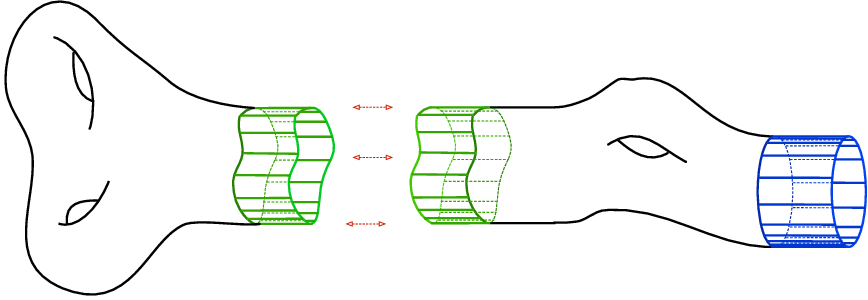
\includegraphics[scale=0.2]{figures/collar.png}
    \caption{Gluing manifolds with collars.}
    \label{fig:collars}
\end{figure}

\begin{defn}[Collar]
    The embedded submanifold $\varPhi(\mathcal{O}_p)$ of a manifold $M$ with a boundary constructed above is called a collar of $M$.
\end{defn}

\begin{cor}
    By varying $t$, we find from the above construction that $M$ is homotopy equivalent to $\mathring{M}$.
\end{cor}

Now, if we have two manifolds $M$ and $N$ with diffeomorphic boundaries, so that
\[h:\partial M\to \partial N\text{ -- diffeomorphism},\]
then we can introduce two collar embeddings (which are also diffeomorphism onto their images)
\[
\alpha:[0,1)\times\partial M\to V\subset M,\quad
\beta:[0,1)\times\partial N\to W\subset N,
\]
and unite them by
\[
\varPhi: V\sqcup W\to \partial M\times (-1,1),\quad \varPhi(x)=
\begin{cases}
(p,-t),& x=\alpha(p,t)\in V,\\
(h(q),t),& x=\beta(q,t)\in W.
\end{cases}
\]
Clearly $\varPhi$  is a topological embedding with a closed image (it's surjective), therefore, $\varPhi$ is a closed mapping.

Now let $\pi:M\sqcup N\to X$ be the quotient map on whose fibers $\varPhi$ is constant. Then $\varPhi$ descends to $\wt{\varPhi}:X\to [-1,1]\times\partial M$. $\varPhi$ is continuous and bijective, $\wt{\varPhi}(K)=\varPhi(\pi^{-1}(K))$ is closed for any compact $K$ (because $\varPhi$ is closed and $\pi$ is continuous), so $\wt{\varPhi}$ is closed too. Therefore, $\wt{\varPhi}$ is a homeomorphism and therefore, a diffeomorphism, and $X$ is a quotient manifold. Alternatively, this follows from the \emph{closed graph theorem}, which states that the graph of any continuous mapping into a Hausdorff space is closed.

\begin{defn}[Gluing of manifolds]
    The construction described above is called the gluing of two manifolds with diffeomorphic boundaries, denoted by $M\cup_h N$. See Figure~\ref{fig:collars}.
\end{defn}

\begin{defn}[Connected sum]\index{Connected sum of manifolds}
    Let $M_i$, $i=1,2$ be two connected manifolds without boundaries and $M_i'=M_i\setminus U_i$, where $U_i$ is a coordinate ball. We can pick two diffeomorphisms $h_i:\partial M_i'\to \bbS^{n-1}$, $i=1,2$. Then we define the connected sum as the gluing along $h_1\circ h_2^{-1}$:
    \[M_1 \# M_2\coloneqq M_1'\cup_{h_1\circ h_2^{-1}}M_2'.\]
\end{defn}
\begin{example}
    $D(M)=M\cup_{\partial M}M$ is called the \emph{double} of a manifold with a boundary.
\end{example}
\begin{example}
    If $X\parallel \partial D$, $D\subset M$, then $\Fl^X$ leaves $D$ invariant.
\end{example}
\begin{cor}
    If $X\parallel \partial M$, then the theorem about the existence of flows applies to $X$.
\end{cor}
\begin{proof}
    Extend $X$ to the double $D(M)$, apply the flow theorem there, then restrict to $M$.
\end{proof}

\begin{thm}[Rectification of vector fields]\index{Theorem!Rectification of vector fields}\label{rectification}
If $X\in\fX(M)$ and $X(p)\neq 0$, then there exists a local chart $(U,\varphi)$ at $p$ such that its slice $S=\{p\in U\mid \varphi^1(p)=0\}$ is diffeomorphic to $\bbD^{n-1}$, $X(p)\notin \T_p S$ and $X=\partial_1$ on $U$.
\end{thm}
\begin{proof}
    Since $S\emb M$, it has a slice neighborhood. We can parametrize $S$ by an embedding map $x:\Omega\to S$ with $\Omega\mathring{\subset}\bbR^{n-1}$. We can take $U$ such that $\restr{X}{U}\cap \T S=\varnothing$. 

    Now we can use a flow-out along $X$ so that the flow $\Fl^X_t(x(s))$ parametrizes $\Fl(x(\Omega))\emb M$. This is a diffeomorphism $\mathcal{O}_\delta\to F(x(\Omega))=x(\Omega)_\delta$ and hence has a smooth inverse. The inverse then gives a local chart $\varphi=\psi^{-1}$, where $\psi(s,t)=\Fl^X_t(x(s))$. Finally, $X=\partial_t=\partial_1$ in this local chart.
\end{proof}

\begin{defn}[Complete integral]\index{Complete integral}\label{def complete integral}
    A complete integral of a vector field $X\in \fX(M)$, $\dim M=n$, is a local function $\varPsi:U\times I_\epsilon\to\bbR^n$ such that $\varPsi^{-1}(\bf{c})$ for every $\bf{c}\in\bbR^n$ in the image of $\varPsi$ is an integral curve of $X$ at a point $m\in U$. The components $\varPsi^i:U\times I_\epsilon\to \bbR$ of this map are called a \emph{complete set of integrals of motion} for $X$.
\end{defn}
\begin{prop}
    Local complete integrals exists for all vector fields.
\end{prop}
\begin{proof}
    First rectify the vector field, then the coordinates $\bf{c}=(\varphi^1(s),\varphi^2(s),\ldots,\varphi^n(s))$ of the point $s$ of intersection of each integral curve with the slice $S$ will be the (constant) value of the diffeomorphism $\varPsi:(s,t)\mapsto \varphi(\Fl_t(s))$ on this whole curve.
\end{proof}




\section{Vector fields as differential operators}

Recall that Lie derivatives of functions satisfy $\Lie_{F_\ast X}F_\ast f=F_\ast\Lie_X f$ for diffeomorphisms $F$. Also, Lie derivatives are local: for any open set $U\subset M$,
\[\Lie_{\restr{X}{U}}\left(\restr{f}{U}\right)=\restr{\left(\Lie_X f\right)}{U}.\]

\begin{defn}[Derivations]\index{Derivation}
    If $A$ is an algebra over a field $\bbK$, then a derivation on $A$ is a $K$-linear map $D:A\to A$ that satisfies the Leibniz rule
    \[D(a\cdot b)=D(a)\cdot b+a\cdot D(b),\;\; a,b\in A.\]
    Is is easy to check that the vector space of all derivations on $A$, denoted by $\mathrm{Der}(A)$, is a Lie algebra under the commutator $[D_1,D_2]=D_1\circ D_2-D_2\circ D_1$.
    An algebra with a distinguished derivation is called a \emph{differential algebra}.\index{Differential algebra}
\end{defn}

Clearly any Lie derivative $\Lie_X, X\in\fX(M)$, is a derivation on the algebra of functions $C^\infty(M)$, because it is a directional derivative in local coordinates.
Moreover, any derivation $D$ on $C^\infty(M)$ satisfies $D(1)=0$, because
\[D(1)=D(1^2)=D(1)\cdot 1+1\cdot D(1)=2\cdot D(1).\]
Finally, the set of all Lie derivatives $\{\Lie_X\}_{X\in\fX(M)}$ is a $C^\infty(M)$-module:
\[f\cdot\Lie_X=\Lie_{f\cdot X}.\]

\begin{prop}[{{\cite[Prop.~2.2.9]{Marsden}}}]\label{prop 2.2.9 Marsden}
    The vector space of Lie derivatives $\{\Lie_X\}_{X\in\fX(M)}$ is isomorphic to $\fX(M)$ as $C^\infty(M)$-modules. In particular, $\Lie_X=0$ iff $X=0$.
\end{prop}
\begin{proof}
    The map $X\mapsto \calL_X$ is clearly $C^\infty(M)$-linear and surjective by definition. To show that it is an isomorphism, we need to show that its kernel is zero. Suppose $\calL_X=0$ and $m\in M$. Then $\dd_m f(X_m)=0$ for all $f\in C^\infty(M)$, and hence $\alpha_m(X_m)=0$ for all $\alpha_m\in \T_m^\ast M$. But then $X_m=0$.
\end{proof}
\begin{prop}[{{\cite[Thm.~2.2.10]{Marsden}}}]\label{lie derivatives and vector fields}
The space of all $\bbR $-linear derivations on the algebra $C^\infty(M)$ is isomorphic to $\fX(M)$ as a vector space. In particular, every derivation $\theta$ coincides with $\Lie_X$ for a unique $X\in\fX(M)$.
\end{prop}
\begin{proof}
    Given $\theta$, we construct the vector field $X$.
    First of all, $\theta$ is local, i.e., if $h$ vanishes on a neighborhood $V\mathring{\subset} M$ of $p\in V$, then $\theta(h)(p)=0$. Indeed, if $\chi$ is a bump function equal to $1$ around $p$ and zero outside of $V$, then $h=(1-\chi)h$ and
    \[\theta(h)(p)=(\theta(1-\chi))\cdot h(p)+\theta(h)\cdot (1-\chi(p))=0.\]

    Pick a local chart at $p$, $\varphi:U\to\wh{U}\subset\bbR^n$. Let $\bf{x}\in\wh{U}$, $\bf{a}=\varphi(p)$, $f\in C^\infty(M)$, then 
    \[(\varphi_\ast f)(\bf{x})=(\varphi_\ast f)(\bf{a})+\sum_{j=1}^n (x^j-a^j)\int_0^1 \frac{\partial(\varphi_\ast f)}{\partial x^j} (\bf{a}+t(\bf{x}-\bf{a}))\dd t\]
    on some neighborhood of $\bf{a}$.
    Therefore, for $u\in U$,
    \[f(u)=f(p)+\sum_{i=1}^n (\varphi^i(u)-a^i)g_i(u),\quad g_i(p)=\frac{\partial(\varphi_\ast f)}{\partial x^i} (\varphi(p)).\] 
    Thus,
    \[(\theta f)(p)=\sum_i g_i(p)\theta(\varphi^i)(p)=\sum \partial_{x^i}(\varphi_\ast f)(\bf{a}) \theta \varphi^i(p),\]
    and this is formula is chart-independent! Now we can define a smooth $X$ by its local representation
    \[X^i(u)\coloneqq \theta\varphi^i(u).\]
    It is easy to check that $X$ is independent of the choice of $\varphi$, which means that it is actually a globally well-defined vector field on $M$. For $f\in C^\infty(M)$, the local representative in $\bf{x}=\varphi(u)\in\wh{U}$ of $\Lie_X f$ is 
    \[(f\circ\varphi^{-1})_{\ast \bf{x}}\circ \wh{X}(\bf{x})=\sum_i \partial_{x^i}(f\circ \varphi^{-1})(x)\cdot \theta \varphi^i (u)=\theta f(u),\]
    hence $\theta=\Lie_X$.
    Uniqueness follows from the obvious statement that $\Lie_X=0$ iff $X=0$.
\end{proof}
\begin{cor}
    If $x^i$ is a local coordinate system, then the local vector fields $\partial_i=\partial_{x^i}$ form a basis of derivations at $p$, therefore, 
    \[(\Lie_X f)(p)=\sum_i \partial_{x^i}(f\circ\varphi^{-1})(\varphi(p))\cdot \underbrace{\Lie_X (\varphi^i)(p)}_{X^i}=\sum_i X^i \partial_{x^i}(\varphi_\ast f)=\sum_i X^i \partial_{i} f.\]
\end{cor}

\begin{prop}
    If $X,Y\in\fX(M)$, then $[\Lie_X,\Lie_Y]=\Lie_X\Lie_Y-\Lie_Y\Lie_X$ is a derivation on $C^\infty(M)$.
\end{prop}
\begin{proof}
    This is a very general property that the commutator of two derivations is always a derivation:
    \begin{multline}
        [D_1,D_2](fg)=D_1((D_2f)g+f(D_2g))-D_2((D_1f)g+f(D_1g))=\\=([D_1,D_2]f)g+f([D_1,D_2]g).
    \end{multline}
\end{proof}

This proposition allows us to define the commutator of vector fields.

\begin{defn}[Lie derivative/bracket of vector fields]\index{Lie derivative!of a vector field}\index{Commutator of vector fields!see {Lie derivative}}
    If $X,Y\in\fX(M)$, then the Lie derivative of $Y$ along $X$ is denoted by 
    \[\Lie_X Y\equiv [X,Y]\] and is defined as the unique vector field such that
    \[\Lie_{[X,Y]}=[\Lie_X,\Lie_Y].\]
    With this bracket, $\fX(M)$ becomes a Lie algebra that is isomorphic to the Lie algebra of derivations on $C^\infty(M)$ (i.e., Lie derivatives).
    In local coordinates (using Einstein summation),
    \[[X,Y]^j=X^i \partial_i Y^j-Y^i \partial_i X^j.\label{eq Lie derivative in components}\]
\end{defn}

\begin{prop}\label{prop properties of Lie derivatives}
\begin{enumerate}
    \item $[X,Y]$ is local and natural w.r.t.\ diffeomorphisms, i.e., \[F_\ast [X,Y]=[F_\ast X,F_\ast Y];\]
    \item $\Lie_X$ is a derivation on the Lie algebra $\fX(M)$, i.e., satisfies the Jacobi identity
    \[\Lie_X [Y,Z]=[\Lie_X Y,Z]+[Y,\Lie_X Z];\]
    \item $\Lie_X$ is also a derivation on $C^\infty(M)\otimes \fX(M)$ i.e., it satisfies the mixed Leibniz rule
    \[\Lie_X(f\otimes Y)=\Lie_X(f\cdot Y)=(\Lie_X f)\cdot Y+f\cdot \Lie_X Y.\]
    Equivalently, 
    \[\Lie_{fX}Y=f\cdot \Lie_X Y+\left(\Lie_X f\right)\cdot Y.\label{Lie derivative not covariant}\]
\end{enumerate}
\end{prop}
\begin{proof}
    \begin{enumerate}
        \item To prove any of these properties, we act with both sides on a function $f$ as a Lie derivative. Then the equality of the two expressions as derivations implies the equality as vector fields by Proposition~\ref{lie derivatives and vector fields}. Therefore, this is just a direct computation using the push-forward property for Lie derivatives acting on functions.
        \item General property of derivations that is easily checked by expanding both sides.
        \item Check 
        \begin{multline}
            [X,fY]g=\Lie_X (\Lie_{fY}g)-\Lie_{fY}\Lie_X g=\Lie_X (f\Lie_Y g)-f\Lie_Y \Lie_X g=\\=(\Lie_X f)\Lie_Y g+f\Lie_X\Lie_Y g-f\Lie_Y\Lie_X g=((\Lie_X f)Y+f[X,Y])g.
        \end{multline}
    \end{enumerate}
\end{proof}


\begin{rem}[Lie derivatives are not covariant derivatives]\label{rem: Lie derivatives not covariant}
    Property \eqref{Lie derivative not covariant} shows that $\Lie_X Y$ doesn't behave like a tensor w.r.t.\ $X$ (or $Y$), since it is not $C^\infty(M)$-linear in it. This is why Lie derivatives are not a special case of \emph{covariant} derivatives.
    
    A covariant derivative (of vector fields) is a map $\nabla:\fX(M)\otimes\fX(M)\to \fX(M)$ denoted by $X,Y\mapsto \nabla_X Y$ such that it satisfies:
    \begin{itemize}
        \item $C^\infty(M)$-linearity in $X$: $\nabla_{fX}Y=f\cdot \nabla_X Y$ for $f\in C^\infty(M)$;
        \item $\bbR $-linearity in $Y$: $\nabla_X (\alpha Y+Z)=\alpha \nabla_XY+\nabla_XZ$ for $\alpha\in\bbR $;
        \item Leibniz rule: $\nabla_X(f\cdot Y)=(\Lie_X f)\cdot Y+f\cdot \nabla_X Y.$
    \end{itemize}
    Therefore, any covariant derivative $\nabla_X Y$ has to be a tensor in $X$, unlike Lie derivatives. In other words, a covariant derivative can be thought of as a map $\nabla:\fX(M)\to \fX^\ast(M)\otimes\fX(M)=\Gamma^1_1(M)$, $Y\mapsto \nabla Y\in\Gamma^1_1(M)$.
\end{rem}

All of this allows us to extend the Lie derivative to tensor fields of any rank by the following theorem.

\begin{defn}[Tensor differential operators]\index{Differential operator on the tensor algebra}
    A differential operator on the tensor algebra $\Gamma^\infty(M)$ is a collection of maps $\mathbb{D}^r_s(U):\Gamma^r_s(U)\to \Gamma^r_s(U)$ for all $r,s\geq 0$ and each open $U\mathring{\subset}M$ (we denote them all by $\mathbb{D}$) such that:
\begin{enumerate}
    \item $\mathbb{D}$ is a tensor derivation (w.r.t.\ $\otimes$);
    \item $\mathbb{D}$ is local, i.e., for $U\subset V$ and $t\in\Gamma^r_s(V)$, $\restr{\mathbb{D}(t)}{U}=\mathbb{D}(\restr{t}{U})$;
    \item $\mathbb{D} \delta=0$, where $\delta\in\Gamma^1_1(M)$ is the Kronecker tensor $\delta=\id_{\T M}$.
\end{enumerate}
\end{defn}

Note that we don't require $\mathbb{D}\circ\varphi_\ast=\varphi_\ast\circ \mathbb{D}$ because this will not hold for covariant derivatives, which we would still like to consider differential operators.

\begin{thm}[Willmore {{\cite[Thm.~2.2.17]{Marsden}}}]\index{Theorem!Willmore}\label{Willmore}
    A collection of local tensor derivations $E_U$ on $C^\infty(U)$ and $F_U$ on $\fX(U)$ (which agree with each other via the mixed rank Leibniz rule) for each $U\mathring{\subset}M$ determines a unique differential operator $\mathbb{D}$ on the tensor algebra $\Gamma^\infty(M)$ that coincides with $E_U$ on $C^\infty$ and with $F_U$ on $\fX$.
\end{thm}
\begin{proof}
    Suppose we know that such a $\mathbb{D}$ exists. In a local frame $\{e_i\}$ and dual frame $\{\alpha^i\}$, we can write
    \[t(u)=\underbrace{t_{j_1\ldots j_s}^{i_1\ldots i_r}(u)}_{\in C^\infty(U)} e_{i_1}\otimes \cdots \otimes e_{i_r}\otimes \alpha^{j_1}\otimes \cdots\otimes \alpha^{j_s}(u).\label{535}\]
    By using the tensorial Leibniz rule for $\mathbb{D}$, we express $\mathbb{D}t(u)$ only in terms of $E_U(t_{j_1\ldots j_s}^{i_1\ldots i_r})$ and $F_U(e_{i_k})$.
    
    Namely, since $\mathbb{D}\delta=0$, and $\delta=e_j\otimes \alpha^j$ (using Einstein summation), we have 
    \[0=\mathbb{D}(e_j\otimes \alpha^j)=(\mathbb{D}e_j)\otimes \alpha^j+e_j\otimes (\mathbb{D}\alpha^j).\]
    Since $\delta^i_j=\alpha^i(e_j)$, if we contract the formula above with $e_i$, we get
    \[0=F_U e_i+(\mathbb{D}\alpha^j)(e_i) e_j,\]
    which completely determines $\mathbb{D}\alpha^j$. Therefore, the action of $\mathbb{D}$ on $\fX^\ast$ is uniquely determined, and the Leibniz rule applied to \ref{535} gives a formula for $\mathbb{D}$ in terms of $E_U$ and $F_U$ on the whole tensor algebra.
    
    The formulas we have derived prove the uniqueness of $\mathbb{D}$. Its existence follows from the fact that these same formulas define a valid differential operator that satisfies all the requirements of the theorem.
\end{proof}
\begin{cor}\label{cor willmore formula}
    A byproduct of the theorem above is the general formula for differential operators on the tensor algebra:

    \begin{multline}
        \mathbb{D}\left(t(\alpha^1,\ldots,\alpha^r,X_1,\ldots,X_s)\right)=(\mathbb{D}t)(\alpha^1,\ldots,\alpha^r,X_1,\ldots,X_s)+\\+\sum_{j=1}^r t\left(\alpha^1,\ldots,\mathbb{D}\alpha^j,\ldots,\alpha^r,X_1,\ldots,X_s\right)+\sum_{k=1}^s t\left(\alpha^1,\ldots,\alpha^r,X_1,\ldots,\mathbb{D}X_k,\ldots,X_s\right).
    \end{multline}
    This formula essentially states that $\mathbb{D}$ ``commutes with contractions''.
\end{cor}

This allows us to extend the definition of the Lie derivative to arbitrary tensor fields. This natural operator was first formalized by \'Elie Cartan around 1920, although he was primarily interested in derivatives of differential forms, which we will study in \S\ref{sec: differential forms}. It was named after Sophus Lie by others in the 1930's.

\begin{defn}[Lie derivatives of tensors]\index{Lie derivative!of a tensor field}
    If $X\in\fX(M)$ then the Lie derivative operator $\Lie_X$ on the tensor algebra $\Gamma^\infty(M)$ is defined as the unique tensor differential operator (established by Willmore's theorem) that coincides with the previously constructed Lie derivative on $C^\infty(M)$ and $\fX(M)$.
\end{defn}

\begin{prop}[Naturality of Lie derivatives]\label{pullbacks of Lie derivatives}
For a diffeomorphism $F$, 
\[\Lie_{F_\ast X}(F_\ast t)=F_\ast (\Lie_X t).\]
\end{prop}
\begin{proof}
    Define an operator $\mathbb{D}$ by $\mathbb{D}t=F^\ast \Lie_{F_\ast t}(F_\ast t)$. We know that $\mathbb{D}$ coincides with $\Lie_X$ on $C^\infty$ and $\fX(M)$. It is also easy to check that $\mathbb{D}$ is a tensor differential operator (exercise). Then, by Willmore's Theorem, is must coincide with $\Lie_X$ on the entire tensor algebra.
\end{proof}





\section{Geometric approach to Lie derivatives}

We now demonstrate a more fundamental geometric definition of Lie derivatives. It has to do with the fact that tensor fields on a manifold $M$, unlike sections of general \glspl{vb} over $M$, can be transformed to other tensor fields by diffeomorphisms of $M$. Thus, infinitesimal diffeomorphisms (i.e., vector fields) produce special differential operators acting on tensor fields.

Let $X\in \fX(M)$ and let $(U,a,F)$ be a flow box of $X$ at $p\in M$. Let $t\in\Gamma^r_s(M)$ and define
\[t_\lambda\coloneqq F_{\lambda}^\ast \left(\restr{t}{U_\lambda}\right)=F_{\lambda\ast}^{-1} \left(\restr{t}{U_\lambda}\right)\in\Gamma^r_s(U),\]
where $F_\lambda :U\to U_\lambda$ is the flow diffeomorphism. Then with fixed $p$, the map $\lambda\mapsto t_\lambda (p) \in \bbT^r_s (\T_p M)$ defines a curve in the vector space of tensors at $p$.
\begin{thm}
    $\lambda\mapsto t_\lambda (p)$ defined above is a curve in the vector space $\bbT^r_s (\T_p M)$ passing through $t(p)$ and its derivative evaluates the Lie derivative of $t$:
    \[\Lie_X t(p)=\restr{\frac{\dd}{\dd \lambda}}{\lambda=0}t_\lambda(p).\]
\end{thm}
\begin{proof}
    We have 
    \[t_\lambda(p)=(\bbT^r_s F_\lambda^{-1})\circ t \circ F_\lambda(p),\] 
    which is clearly smooth.
    Define $\theta_X$ as an operator on $\Gamma^r_s(M)$ by 
    \[\theta_X t(p)=\restr{\frac{\dd}{\dd \lambda}}{\lambda=0} t_\lambda(p).\]
    For $t\in C^\infty(M)$, $t_\lambda(p)$ is smooth, therefore, $\theta_X t(p)=(Tt_\bullet)(\partial_\lambda)\in C^\infty(M)$, where the differential $T$ is w.r.t.\ the variable $\lambda$ (represented by $\bullet$) and  $\partial_\lambda$ is a vector field on the $\bbR $. $\theta_X$ is a linear derivation because its local representatives are. It is defined locally, therefore, it is local. Finally, 
    \[\theta_X\delta=\restr{\frac{\dd}{\dd \lambda}}{\lambda=0} F^\ast_\lambda \delta=\restr{\frac{\dd}{\dd \lambda}}{\lambda=0}\delta=0.\] 
    This proves that $\theta_X$ is a differential operator. It remains to check that $\theta_X=\Lie_X$ on $C^\infty(M)$ and $\fX(M)$. First, for $f\in C^\infty(M)$, 
    $f_\lambda=f\circ F_\lambda$, 
    \[\restr{\frac{\dd}{\dd \lambda}}{\lambda=0}f_\lambda(p)=\dd f\circ \restr{\frac{\dd}{\dd \lambda}}{\lambda=0}F_\lambda=\dd f\circ X=\Lie_X f.\]
    Now, note that for $f\in C^\infty(M)$ there exists a $g_\lambda\in C^\infty(M)$ such that $g_0=\Lie_X f$ and $f\circ F_\lambda=f+\lambda g_\lambda$. Namely, 
    \[\lambda g_\lambda (p)=\int_0^1 \partial_t(f\circ F_{t\lambda}(p))\dd t.\] 
    Then for $Y\in\fX(M)$,
    \begin{align}
        \Lie_{\theta_X Y}f(p)&=\dd f\circ \restr{\frac{\dd}{\dd \lambda}}{\lambda=0} \left((F_{-\lambda})_{\ast p}\circ Y\circ F_\lambda(p)\right)=\\
        &=\restr{\frac{\dd}{\dd \lambda}}{\lambda=0}\left((f\circ F_{-\lambda})_\ast\circ Y\circ F_\lambda(p)\right)=\\
        &=\restr{\frac{\dd}{\dd \lambda}}{\lambda=0} \left((f-\lambda g_{-\lambda})_\ast\circ Y\circ F_\lambda(p)\right)=\\
        &=\restr{\frac{\dd}{\dd \lambda}}{\lambda=0} f_\ast\circ Y\circ F_\lambda (p)-\restr{\left(\frac{\dd}{\dd \lambda}\lambda\right)(g_{-\lambda})_\ast\circ Y\circ F_\lambda(p)}{\lambda=0}=\\
        &=\dd(\underbrace{f_\ast\circ Y}_{\Lie_Yf})\circ \underbrace{\restr{\frac{\dd}{\dd \lambda}}{\lambda=0} F_\lambda(p)}_{X(p)}-(g_0)_\ast \circ Y\circ F_0(p)=\\
        &=\Lie_X\Lie_Y f-\Lie_Y\Lie_X f(p),
    \end{align}
    therefore, $\theta_X Y=[X,Y]$. By Willmore's theorem, $\theta_X=\Lie_X$.
\end{proof}
\begin{cor}
\begin{enumerate}
    \item $\Lie_X t=0$ iff $t$ is constant along the flow of $X$: $F^\ast_\lambda t=t$;
    \item For all $\lambda$ in the flow domain the following equality holds:
    \[\frac{\dd}{\dd \lambda}F^\ast_\lambda t=F^\ast_\lambda \Lie_X t.\]
    In particular, 
    \[\Lie_X t=F^\ast_{-\lambda} \frac{\dd}{\dd \lambda}F^\ast_\lambda t=\restr{\frac{\dd}{\dd\lambda}}{\lambda=0}F^\ast_\lambda t.\]
\end{enumerate}
\end{cor}

\begin{rem}[Push-forwards are not parallel transports]
    Since covariant derivatives are in the exact same relationship with parallel transports as Lie derivatives are with push-forwards, it is tempting to think that Lie derivatives are special cases of covariant derivatives. However, we have already seen this to be wrong in Remark \ref{rem: Lie derivatives not covariant}. This means that push-forwards by flows of vector fields cannot be interpreted as a kind of parallel transport along the integral curves of those vector fields. This is because a parallel transport has to be unambiguously defined for every curve on $M$, whereas there are infinitely many vector fields for which a given curve is integral (and the value of the push-forward will depend on the specific choice of vector field). Transport by push-forwards is often called \emph{Lie transport}\index{Lie transport}. Lie derivatives are just infinitesimal Lie transport.
\end{rem}

\begin{rem}
    We can apply these ideas to PDEs on $\bbR^n$:
    \[\begin{cases}
        \partial_t f(x,t)=\sum _i X^i \partial_i f(x,t),&\\
        f(x,0)=g(x).&
    \end{cases}\]
    Then if $X$ has a complete flow $F_t$, the unique solution of the above Cauchy problem is $f(x,t)=g(F_t(x))$, which can be checked by substitution. This is sometimes called the \emph{method of characteristics}. The ``characteristics'' are the integral curves along which the values of $g(x)$ get propagated.
\end{rem}

\begin{prop}
    Given two vector fields $X,Y$ with complete flows $F_t$ and $G_t$, respectively, \gls{tfae}:
    \begin{enumerate}
        \item $[X,Y]=0$;
        \item $F^\ast_t Y=Y$ (or $G^\ast_t X=X$);
        \item $F_t\circ G_s=G_s\circ F_t$ for all $t,s$. 
    \end{enumerate}
    In particular, the flow of $X+Y$ for commuting $X$ and $Y$ is $F_t\circ G_t$.
\end{prop}
\begin{proof}
    $1\implies 2$. $\frac{\dd}{\dd t}F^\ast_t Y=F^\ast_t \Lie_X Y=0$, therefore, $F^\ast_t Y$ is constant and we know that $F^\ast_0 Y=Y$, so $F^\ast_t Y=Y$.

    $2\implies 3$. Consider the curve $\gamma(t)=G_s\circ F_t(p)$. It starts at $\gamma(0)=G_s(p)$ and its velocity is
    \[\dot\gamma(t)=\frac{\dd}{\dd t} G_s\circ F_t(p)=G_{s\ast}\circ X\circ F_t\overset{(2)}{=}X\circ\gamma(t).\]
    So $\gamma(t)$ is an integral curve of $X$ going through $p$. Therefore, by uniqueness (and definition of the flow of $X$), 
    \[\gamma(t)=F_t\circ G_s(p).\]
    This shows that the flows commute. Finally, we check 
    \[\frac{\dd}{\dd t} F_t\circ G_t(p)=X(F_t(G_t(p)))+\underbrace{F_{t\ast }Y}_{Y\circ F_t}(G_t(p))=(X+Y)(F_t\circ G_t(p)).\]

    $2\implies 1$. $\Lie_X Y=F^\ast_{-t}\frac{\dd}{\dd t}F^\ast_t Y=F^\ast_{-t} \frac{\dd}{\dd t}Y=0$.

    $3\implies 2$. $F_{t\ast}Y=F_{t\ast}\frac{\dd}{\dd s}G_s=F_{t\ast} G_{s\ast} Y=(F_t\circ G_s)_\ast Y=(G_s\circ F_t)_\ast Y=G_{s\ast}F_{t\ast}Y$. But the only vector field invariant under $G_{s\ast}$ is $Y$, therefore, $F_{t\ast}Y=Y$.
\end{proof}

\begin{rem}[Taylor formula on manifolds]\index{Taylor's formula}\label{rem 3.2.9 RS1}
    Successive application of the vector fields $X_1,\ldots,X_r$ to a function $f\in C^\infty(M)$ yields
    \[X_r\cdots X_1 \cdot f=\restr{\frac{\dd}{\dd t_1}}{t_1=0}\cdots \restr{\frac{\dd}{\dd t_r}}{t_r=0}f\circ F^{X_1}_{t_1}\circ \cdots \circ F^{X_r}_{t_r}.\]
    In particular, the Lie bracket can be expressed as
    \[[X,Y]f=\restr{\frac{\dd}{\dd t}}{t=0}\restr{\frac{\dd}{\dd s}}{s=0}\left(f\circ \Fl^Y_s\circ \Fl^X_t-f\circ \Fl^X_s\circ \Fl^Y_t\right).\label{eq Lie bracket in terms of flows}\]
    Furthermore, for any $m\in M$, the Taylor expansion of the smooth function $t\mapsto f\circ \Fl^X_t(m)$ at $t=0$ yields the following \emph{Taylor formula for manifolds}:
    \[f\circ \Fl^X_t(m)=\sum_{k=1}^n\frac{t^k}{k!}\left(X^kf\right)(m)+\calO(t^{n+1}), \quad t\in \calD^X_m,\label{eq:Taylor formula for manifolds}\]
    where $\calO(t^{n+1})$ is a smooth function on $\calD_m^X$ such that $\calO(t^{n+1})/t^{n+1}$ is bounded. By defining the exponential of a differential operator formally as $\rme^{tD}=\sum_{k=0}^\infty \frac{t^k}{k!}D^k$, the above Taylor formula is sometimes written formally as $f\circ \Fl^X_t=\rme^{t X}\cdot f$.

    Repeated application of this formula yields the iterated Taylor formula for manifolds
    \[f\circ \Fl^X_t\circ \Fl^Y_s(m)=\sum_{k,l=1}^n\frac{t^ks^l}{k!l!}\left(Y^lX^kf\right)(m)+\calO(t^{n+1},s^{n+1}),\label{eq: Taylor formula for two fields}\]
    which easily generalizes to any number of vector fields.
\end{rem}


\begin{defn}[Holonomic frame]\index{Holonomic frame}
    A local $k$-frame $\{e_i\}_{i=1}^k$ is called holonomic if $[e_i,e_j]=0$ for all $i,j$.
\end{defn}

The following shows that this definition of holonomic frames agrees with the one indicated in Definition~\ref{def jet bundles}. That is, each holonomic frame arises from some local coordinates.

\begin{thm}[Rectification of frames]\index{Theorem!Rectification of frames}\label{thm rectification}
    Let $\{e_j\}_{j=1}^k$ with $k\leq n=\dim M$ be a holonomic local $k$-frame on $W\mathring{\subset}M$. Assume that $e_j(p)\notin \T_p S$ for all $p\in S$, where $S\emb M$ is a submanifold with $\codim S=k$. Then there exists a local chart of coordinates $(s^1,\ldots,s^n)$ in which $S=\{s^1=\cdots=s^k=0\}$ and for $j\leq k$ we have $\partial_j=e_j$.
\end{thm}
\begin{proof}
    Parametrize $S$ as usual by $x:\varOmega\to S$ with $\varOmega\mathring{\subset}\bbR^{n-k}$, define a chart $\varphi=\psi^{-1}$, where
    \[\psi(s^1,\ldots,s^k,s^{k+1},\ldots,s^n)=F^{e_1}_{s_1}\circ\cdots\circ F^{e_k}_{s_k}(x(s^{k+1},\ldots,s^n)),\]
    and $F^{e_i}$ is the flow of $e_i$. The inverse $\psi^{-1}$ exists locally because the differential at $(0,\ldots,0)$ is identity. Finally we use commutation to compute the partials
    \begin{multline}
        \psi_\ast (\partial_{s^i})\cdot f=\partial_i(f\circ\psi)=\partial_i f(F^{e_1}_{s_1}\cdots F^{e_k}_{s_k} x(0,\ldots,0,s^{k+1},\ldots))=\\=\partial_i f(F^{e_i}_{s_i}\circ\cdots )=\partial_i F^{e_i}_{s_i}(F\cdots F(0,\ldots,0,s^{k+1},\ldots))f=e_i\cdot f=\Lie_{e_i}f,
    \end{multline}
    thus $\partial_i=e_i$.
\end{proof}

\begin{cor}
    A helpful way to reformulate this theorem for $k=\dim M$ is: a given local frame is a coordinate frame for some local coordinates if and only if it is holonomic.
\end{cor}

The analog of this corollary for $k<\dim M$ is a famous theorem that deserves its own section.





\section{Frobenius theorem I}\label{sec: frobenius i}

We have just established that in the presence of a local holonomic $r$-frame $\{e_i\}_{i=1}^r$ transversal to a submanifold $S$, each point $m\in S$ admits a $r$-dimensional embedded submanifold $N$ passing through $m$ (defined by holding the values of $s^{r+1},\ldots,s^n$ constant) transversally to $S$ such that $\{e_i\}_{i=1}^r$ is a frame for $\T N$. In this \sect\ we will replace holonomic frames by the subspaces of tangent spaces that they span and derive the corresponding \emph{integrability condition}. Namely, while we can think of vector fields as fields of velocities, let us instead think of them as fields of lines, or directions. Then it is easy to generalize the problem as follows: given a field of hyperplanes (subspaces of tangent spaces), what does it mean for a submanifold to be integral for this field, and what is the condition for this kind of integrability?

\begin{hrem*}
    Note that while this theorem is universally named after Frobenius, his result (1887) was an application of an older result to the context of systems of differential equations. We will discuss that version of the theorem in \S\ref{sec: frobenius ii}. The results discussed in this \sect\ were obtained by Deahna (sufficient condition, 1840) and Clebsch (necessary condition, 1866), among many others involved in this long process.
\end{hrem*}

\begin{figure}[tp]
    \centering
    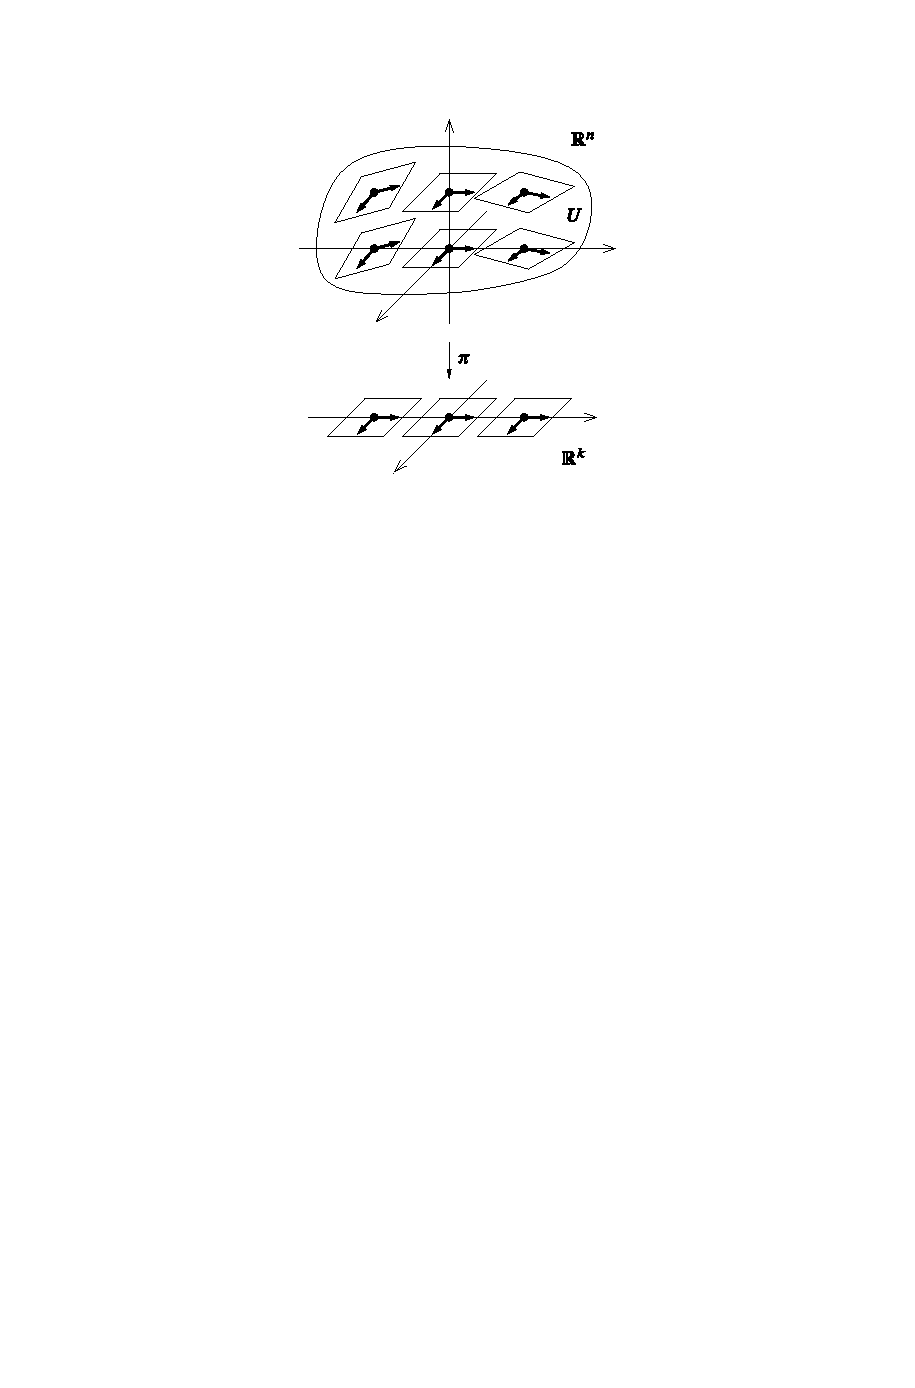
\includegraphics[scale=0.8]{figures/frobenius_1.pdf}
    \caption{Frobenius Theorem. From \cite{Lee}.}
    \label{fig: frobenius1}
\end{figure}

Recall that a distribution $D$ on a manifold is an assignment of a subspace $D_m\subset \T_m M$ for every $m\in M$. If the dimension of $D_m$ is constant and equal to $r$, then $D$ is said to be \emph{regular of rank} $r$. $D$ is called a \emph{smooth distribution} if it is a subbundle of $\T M$.

\begin{defn}[Integral manifolds]\index{Integral manifold}
    Let $D< \T M$ be a smooth distribution (i.e., a subbundle of $\T M$). An immersed submanifold $N<M$ is called an integral manifold of $D$ if $\T_m N=D_m$ for all $m\in N$.
\end{defn}

\begin{defn}[Integrable distribution]\index{Integrable distribution}
    A smooth distribution $D< \T M$ is called (completely) integrable if every $m\in M$ is contained in a (local) integral manifold of $D$.
\end{defn}

\begin{rem}
    Depending on the context, a distribution may also be called integrable if it has integral manifolds of \emph{some} positive dimension at every point. However, we will treat the term ``integrable distribution' as synonymous to ``completely integrable distribution'' unless otherwise specified. Integrability in this broader sense will be properly distinguished from complete integrability in \Chap~\ref{chap: EDSs}.
\end{rem}

\begin{defn}[Involutive distribution]\index{Involutive distribution}
    For a smooth distribution $D< \T M$, denote by $\Gamma^\infty(D)\subset\fX(M)$ the space of $D$-valued vector fields. $D$ is called involutive if $\Gamma^\infty(D)$ is a Lie subalgebra of $\fX(M)$, i.e., $[X,Y]\in\Gamma^\infty(D)$ for all $X,Y\in\Gamma^\infty(D)$.
\end{defn}

\begin{thm}[Frobenius Theorem (Clebsch 1866) {{\cite[Thm.~19.12]{Lee}}}]\index{Theorem!Frobenius}\label{thm frobenius}
    A smooth distribution $D$ is involutive iff it is completely integrable.
\end{thm}
\begin{proof}
    The backwards direction is trivial: if $D$ is integrable, then $D=\T N$ locally, which implies involutivity.
    For the forward direction, it suffices to prove that $D$ is locally spanned by a set of linearly independent commuting fields. Then, by the Rectification Theorem~\ref{thm rectification}, they are coordinate vector fields for a slice chart of an integral manifold.

    Because of the locality of the statement, it also suffices to prove the theorem for $M=U\subset \bbR^n$. Suppose that the rank of $D$ is $r$. Then, at every $m\in M$, we can find a system of Cartesian coordinates such that $D_m$ is complementary to the span $\<\partial_{r+1},\ldots,\partial_m\>$. By continuity, this remains true on some neighborhood of $m$. Therefore, we have a non-singular projection $\pi:\bbR^m\to\bbR^r$ onto the coordinate hyperplane of the coordinates $(x^1,\ldots,x^r)$. Then $\restr{\pi_\ast}{D}$ is a smooth bundle isomorphism, and the vector fields $\pi^\ast(\partial_i)$, $i=1,\ldots,r$, locally span $D$, see Figure~\ref{fig: frobenius1}. By naturality of Lie derivatives, $[\pi^\ast(\partial_i),\pi^\ast(\partial_j)]=\pi^\ast[\partial_i,\partial_j]=0.$
    Thus, $D$ is indeed spanned by a holonomic $r$-frame and therefore, integrable.
\end{proof}

This theorem is of crucial importance in the theory of Lie groups, \glspl{fb}, and even dynamical systems. The entire concept of \emph{integrability} ultimately stems from it. The rest of this \sect\ is devoted to characterizing integral submanifolds and proving a global version of the Frobenius theorem, which will be useful is many applications down the line.

\begin{cor}[{{\cite[Cor.~19.13]{Lee}}}]\label{cor 19.13 Lee}
    Let $D$ be a rank $r$ involutive distribution on $M$. If $S\emb M$ is a codimension $r$ embedded submanifold such that $\T_mS\cap D_m=\{0\}$ for all $m\in S$, then there is a \emph{flat chart}\index{Flat chart} $(U,\{s^i\})$ for $S$ centered at $m$ in which $S\cap U$ is the slice $s^1=\cdots=s^r=0$.
\end{cor}
\begin{proof}
    The proof of Frobenius theorem showed that locally $D$ is spanned by $r$ commuting vector fields, so this corollary follows by the Rectification Theorem~\ref{thm rectification}.
\end{proof}

Note also that $U$ gets decomposed into a disjoint union of integral submanifolds $U_{\bf{c}}$ parametrized by a point $\bf{c}\in S$ with coordinates $(0,\ldots,0,c^1,\ldots,c^{n-r})$ in the flat chart and defined as the slices $s^{r+1}=c^1,\ldots, s^n=c^{n-r}$.

\begin{prop}[{{\cite[Prop~19.16]{Lee}}}]\label{prop 19.16 Lee}
    Let $D$ be an involutive distribution of rank $r$ on a smooth manifold $M$, and let $(U,\{x^i\})$ be a flat chart for $D$. If $N$ is an integral manifold of $D$, then $N\cap U$ is a union of countably many disjoint open subsets of parallel $r$-dimensional slices of $U$, each of which is open in $N$ and embedded in $M$.
\end{prop}
\begin{proof}
    Since the inclusion $i:N\hookrightarrow M$ is continuous, $N\cap U=i^{-1}(U)$ is open in $H$ and this is a countable disjoint union of connected components, each open in $N$.

    Let $V$ be a component of $N\cap U$. Since the chart is flat, the functions $x^{r+1},\ldots,x^n$ are constant along $D$ and therefore, constant on any connected slice like $V$, and $V$ lies in a single slice $U_{\bf{c}}$, see Figure~\ref{fig: frobenius2}.

    Since $U_{\bf{c}}$ is embedded in $M$, the inclusion $V\hookrightarrow M$ also restricts to a smooth map into $U_{\bf{c}}$. The inclusion $V\hookrightarrow U_{\bf{c}}$ is thus an injective smooth immersion between manifolds of the same dimension, and therefore, a local diffeomorphism, an open map, and a homeomorphism onto an open subset of $U_{\bf{c}}$. The inclusion map $V\hookrightarrow M$ is a composition of the smooth embeddings $V\hookrightarrow S\hookrightarrow M$ and thus a smooth embedding.
\end{proof}

Recall now that a weakly embedded submanifold $N<M$ is such that any smooth map into $M$ whose values lie in $N$ restricts to a smooth map into $N$.

\begin{figure}[tp]
    \centering
    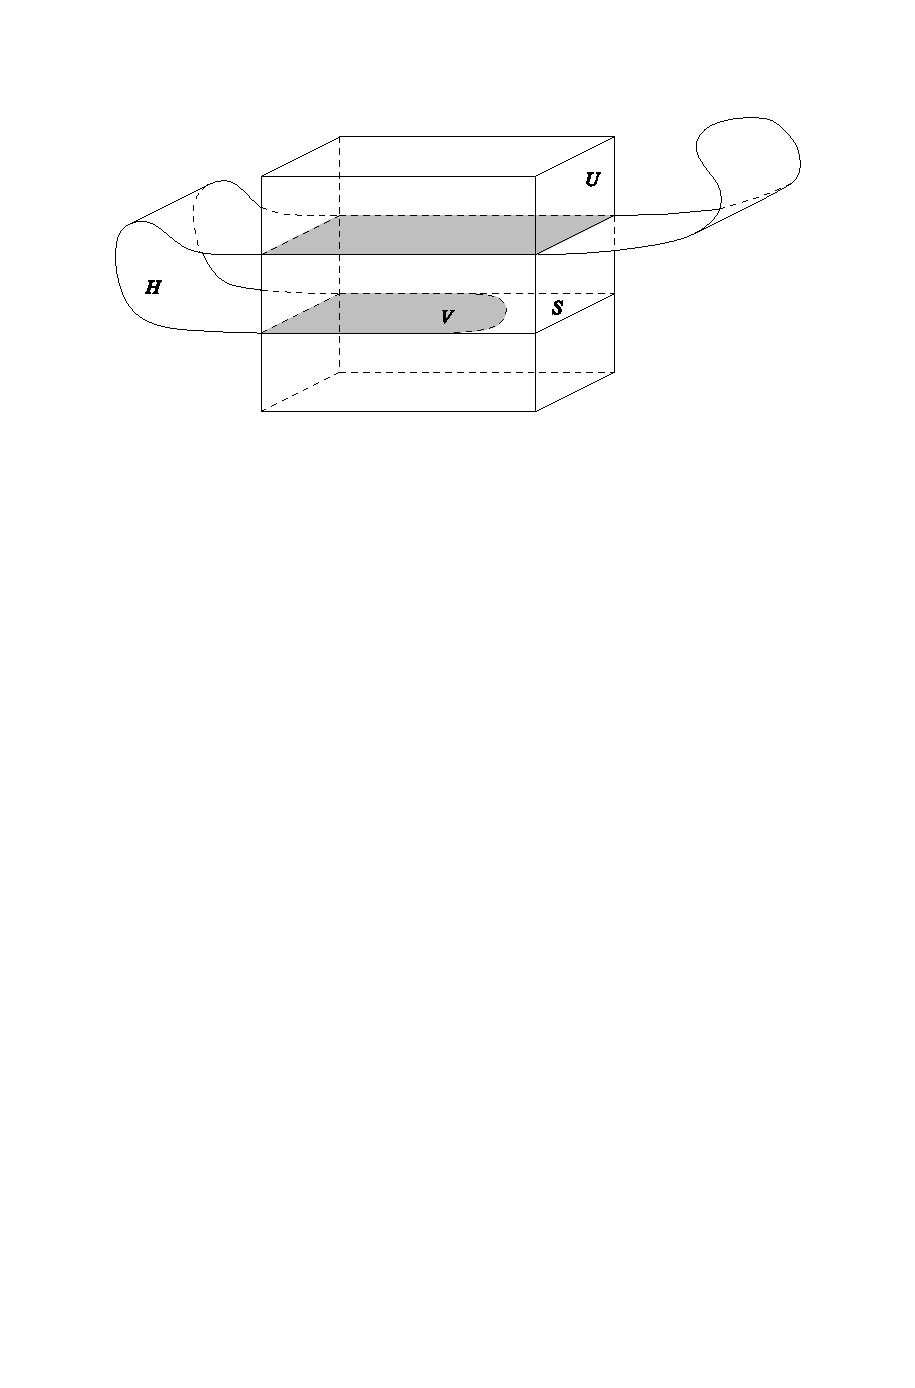
\includegraphics[scale=0.8]{figures/frobenius_2.pdf}
    \caption{Local structure of a leaf in a flat chart. From \cite{Lee}.}
    \label{fig: frobenius2}
\end{figure}


\begin{thm}[{{\cite[Thm.~19.17]{Lee}}} or {{\cite[Prop.~3.5.15]{RS1}}}]\label{thm 19.17 Lee}\label{prop 3.5.15 RS1}
    Every integral manifold of an involutive distribution is weakly embedded.
\end{thm}
\begin{proof}
    Let $N\subset M$ be an integral manifold of an involutive rank-$r$ distribution $D$ on $M$ and let $F:L\to M$ be a smooth map such that $F(L)\subset N$. Choose $p\in L$ and set $m=F(p)\in N$. Let $\{y^i\}_{i=1}^n$ be flat coordinates for $D$ on a neighborhood $U$ of $m$, and let $\{x^i\}$ be smooth coordinates for $L$ on a connected neighborhood $B$ of $p$ such that $F(B)\subset U$. With the coordinate representation of $F$ written as 
    \[y^i=F^i(x),\]
    the fact that $F(B)\subset N\cap U$ means that the functions $F^{r+1},\ldots, F^n$ take on only countably many values. Since $B$ is connected, these coordinate functions are constant, and thus $F(B)$ lies in a single slice $U_{\bf{c}}\subset U$. Because $U_{\bf{c}}\cap N$ is an open subset in $N$ that is embedded in $M$, it follows that $\restr{F}{B}$ is smooth from $B$ into $U_{\bf{c}}\cap N$, and thus by composition, $\restr{F}{B}:B\to U_{\bf{c}}\cap N\hookrightarrow N$ is smooth into $N$.
\end{proof}
\begin{cor}
    Images of the maximal integral curves of a vector field are weakly embedded submanifolds.
\end{cor}




% \begin{rem}
%     The version of the Frobenius theorem proved above is local, i.e., integral submanifolds are guaranteed to exist only in small neighborhoods. However, the full version of the Frobenius theorem is much more powerful as it establishes a bijection between smooth integrable distributions and smooth \emph{foliations} of $M$ by maximal integral submanifolds (analogs of maximal integral curves of vector fields). A foliation is a decomposition of $M$ into a disjoint union of immersed submanifolds, called \emph{leaves}, such that every point has a local chart in which the foliation is flat (i.e., the leaves are just $k$-dimensional hyperplanes of the form $x^{k+1}=c^{k+1},\ldots, x^{n}=c^n$). For a global version of the Frobenius theorem, see \cite[Ch.~19]{Lee} or \cite[\S~3.5]{RS1}.
% \end{rem}


\begin{lem}[{{\cite[Lem.~3.5.14]{RS1}}}]\label{lem 3.5.14 RS1}
    Let $D<\T M$ be a smooth distribution on $M$.
    \begin{enumerate}
        \item Let $N_1,N_2\subset M$ be two integral manifolds of $D$. If $N_1\cap N_2\neq \varnothing$ then $N_1\cap N_2$ is open in $N_1$ and $N_2$ and the smooth structures on it induced from either coincide. There is a unique smooth structure on $N_1\cup N_2$ such that $N_1$ and $N_2$ are open submanifolds. W.r.t.~this structure $N_1\cup N_2$ is an integral manifold of $D$.

        \item Let $N\subset M$ be an integral manifold of $D$, let $m\in M$ such that $\dim D_m=\dim N$ and let $(U,\kappa)$ be a local flat chart for $D$ at $m$. If a slice $U_{\bf{c}}$ of $U$ intersects $N$, then $U_{\bf{c}}$ is an integral manifold of $D$ and $N\cap U_{\bf{c}}$ is open and closed w.r.t.~the topology induced from $N$. In particular, the number of slices of $U$ intersecting $N$ is at most countable.  
    \end{enumerate}
\end{lem}
Note that the number of slices of $U$ intersected by $N$ may, in fact, be countably infinite, as is the case with the ``irrational slope'' vector fields $\partial_x+\lambda\partial_y$, $\lambda\in\bbR\setminus\bbQ$, on the torus $\bbR^2\slash \bbZ^2$.
\begin{proof}
\begin{enumerate}
    \item The assertion on $N_1\cup N_2$ follows from that on $N_1\cap N_2$, so it suffices to prove the latter. Let $\dim N_1=\dim N_2=\rank D=r$. Choose a local $r$-frame $\{X_i\}_{i=1}^r$ for $D$ at $m$. Since these vector fields are tangent to $N_i$, they are also local vector fields on $N_i$. Then the flows of these vector fields together generate a local coordinate system on $N_i$, mapping $(-\epsilon,\epsilon)^r$ into an open subset of $N_i$:
    \[\varPhi^{(i)}:(-\epsilon,\epsilon)^r\to U\cap N_i,\quad \varPhi^{(i)}(\bf{t})\coloneqq \Fl^{X^{(i)}_1}_{t_1}\circ \cdots\circ \Fl^{X^{(i)}_r}_{t_r}(m),\quad i=1,2.\]
    By construction these coordinates will coincide, $\varPhi^{(1)}(\bf{t})=\varPhi^{(2)}(\bf{t})$ (cf.\ Remark~\ref{rem 3.2.9 RS1}), and therefore, their values will cover the same subset $V\subset N_1\cap N_2$ open in both $N_i$'s. W.r.t.~the differentiable structure induced from either $N_i$, $V$ is diffeomorphic to $(-\epsilon,\epsilon)^r$. Since the construction works for any $m\in N_1\cap N_2$, the assertion follows. 

    \item Let $r=\dim N=\dim D_m$. If $N$ intersects a slice $U_{\bf{c}}$, then $U_{\bf{c}}$ contains a point where $\rank D=r$. Then $U_{\bf{c}}$ is an integral manifold of $D$ by dimension-counting. Now assertion 1 implies that $N\cap U_{\bf{c}}$ is open in $N$ and hence in $N\cap U$. Since this holds for all slices intersecting $N$ and since
    \[N\cap U_{\bf{c}}=(N\cap U)\setminus\left(\bigcup_{\bf{c}'\neq \bf{c}}N\cap U_{\bf{c}'}\right),\]
    the intersection $N\cap U_{\bf{c}}$ is also closed in $N\cap U$. It follows that $N\cap U_{\bf{c}}$ is a union of connected components of $N\cap U$. Since the slices are disjoint, this implies that the number of slices which intersect $N$ is at most as large as the number of connected components of $N\cap U$. Since the topology on $N\cap U$ is induced from the manifold $N$, it is second countable, hence the number of connected components is at most countable.
\end{enumerate}
\end{proof}



\begin{thm}[{{\cite[Thm.~3.5.17]{RS1}}}]\label{thm 3.5.17 RS1}
    Let $D$ be an integrable distribution on $M$. For every $m\in M$ there exists a unique integral manifold $N_m$ of $D$ through $m$ which is maximal in the following sense. For every integral manifold $N$ of $D$ such that $N\cap N_m\neq \varnothing$ it holds that $N\subset N_m$, and $N$ is an open submanifold of $N_m$.
\end{thm}
\begin{proof}
    Let $r=\dim D_m$ and define a subset $N_m\subset M$ by taking the union of all integral manifolds of $D$ through $m$. Equip it with the topology generated by the open subsets of these integral manifolds. The onion of all maximal atlases of these manifolds also defines an atlas on $N_m$. By Lemma~\ref{lem 3.5.14 RS1} this atlas is smooth.  One can then show that $N_m$ is second countable (see \cite[Lem.~19.22]{Lee} or \cite[Thm.~1.64]{Warner}). Then $N_m$ is a manifold of dimension $r$. By construction, the local representatives of the inclusion $N_m\hookrightarrow M$ are smooth, hence $N_m$ is a smooth submanifold of $M$. Also by construction, every $\wt{m}\in N_m$ belongs to an integral manifold $N$ through $m$ and $N$ is an open submanifold of $N_m$, so $\T_{\wt m}N_m=\T_{\wt m}N=D_{\wt m}$, and thus $N_m$ is also an integral manifold through $m$. It has the maximality property stated in the theorem because if some integral manifold $N$ of $D$ intersects $N_m$, then $N\cup N_m$ is also integral and thus already contained in $N_m$. It follows that $N\cap N_m=N$ and hence $N$ is an open submanifold of $N_m$. Uniqueness follows because any two maximal integral manifolds through $m$ would coincide as sets by definition and each of them would be an open submanifold of the other, hence they would also coincide as manifolds.
\end{proof}


\begin{defn}[Foliation]\index{Foliation}
    A foliation of an $n$-dimensional smooth manifold $M$ is a family $\mathcal{N}$ of connected submanifolds of $M$, called the \emph{leaves} of the foliation, such that
    \begin{enumerate}
        \item the leaves are disjoint and $\cup_{N\in\mathcal{N}}N=M$,
        \item for every $m\in M$ there exists a local \emph{flat chart} $(U,\kappa)$ of $M$ satisfying
        \begin{enumerate}[label=(\alph*)]
            \item $\kappa(m)=0$ and $\kappa(U)=(-\epsilon,\epsilon)^n$ for some $\epsilon>0$,
            \item the leaves are invariant under the flows of the local coordinate vector fields $\partial_1,\dots,\partial_r$, where $r$ denotes the dimension of the leaf containing $m$, also called the \emph{rank} of $\mathcal{N}$ at $m$.
        \end{enumerate}
    \end{enumerate}
    A foliation is called \emph{regular} if its rank is constant, and singular otherwise.
\end{defn}



\begin{thm}[Global Frobenius Theorem {{\cite[Prop.~3.5.21]{RS1}}} or {{\cite[Thm.~19.21]{Lee}}}]\label{prop 3.5.21 RS1}\index{Theorem!Global Frobenius}
    The collection of all maximal connected integral manifolds of an involutive distribution $D$ on a smooth manifold $M$ forms a foliation of $M$.
    
    The assignment of the family of maximal integral manifolds to an integrable distribution defines a bijection between smooth integrable distributions on $M$ and smooth foliations of $M$. Regular distributions of rank $r$ thereby correspond to regular foliations of rank $r$.
\end{thm}
\begin{proof}
    Theorem~\ref{thm 3.5.17 RS1} implies that condition 1 of the definition of a foliation is satisfied. The invariance of maximal integral manifolds under the flows of local $D$-valued vector fields lets us generate local flat charts via a composition of the flows (as in Rectification Theorem~\ref{rectification}) and hence condition 2 is satisfied as well. 

    Conversely, let $\mathcal{N}$ be a smooth foliation. For $m\in M$, let $D_m$ be the tangent space at $m$ of the leaf containing $m$. This defines a subset $D\subset \T M$. By definition of a foliation, $D_m$ is spanned by the values of local $D$-valued vector fields at $m$. Hence $D$ is a distribution. By construction, every leaf is an integral manifold of $D$. First, this implies that $D$ is integrable. Second, in view of Theorem~\ref{thm 3.5.17 RS1}, this implies that every leaf of $\mathcal{N}$ is contained in an open subset in a maximal integral manifold of $D$. Thus $N$ is a union of leaves. Since the leaves are disjoint and $N$ is connected, $N$ must coincide with a single leaf. This shows that $\mathcal{N}$ is the family of maximal integral manifolds of $D$, and the assignment is bijective, indeed.
\end{proof}



\begin{figure}[tp]
    \centering
    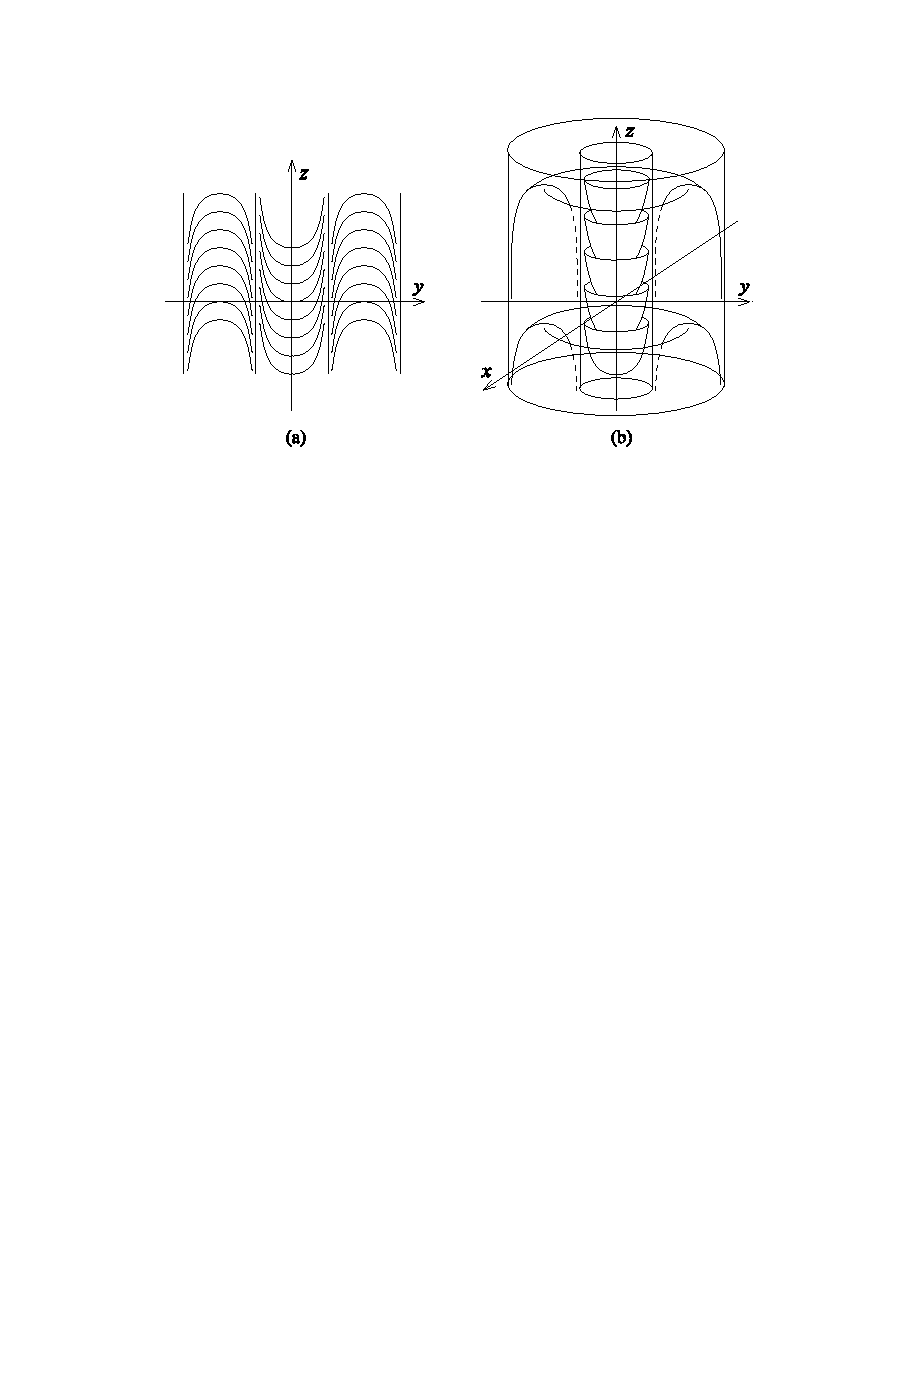
\includegraphics[scale=0.8]{figures/foliations.pdf}
    \caption{Examples of foliations of $\bbR^2$ (a) and $\bbR^3$ (b). From \cite{Lee}.}
    \label{fig:foliations}
\end{figure}

\begin{example}[Linear PDEs]
    Overdetermined systems of linear PDEs are solvable iff the distribution spanned by the differential operators as vector fields is integrable:
    \[\begin{cases}
        X_1\cdot u(x)=f_1(x),&\\
        \cdots &\\
        X_k\cdot u(x)=f_k(x)&
    \end{cases}
    \text{ has solutions iff }\exists\,C^k_{ij}\in C^\infty\text{ s.t.}
    \begin{cases}
        [X_i,X_j]=C^k_{ij}X_k,&\\
        X_i\cdot f_j-X_j\cdot f_i=C^k_{ij}f_k.&
    \end{cases}
    \]
\end{example}

\begin{xca}
    Show that the distribution on $\bbR^3\setminus \{0\}$ generated by the vector fields
    \[X_1=x_2\partial_3-x_3\partial_2,\quad X_2=x_3\partial_1-x_1\partial_3,\quad X_3=x_1\partial_2-x_2\partial_1,\]
    is regular of rank $2$ and involutive. Find the maximal integral manifolds. How are they related to the action of $\SO(3)$ on $\bbR^3$?
\end{xca}


\begin{example}[Zero curvature conditions]\label{ex UV pairs}
    Another important case is the following pair of equations on a function $\bf{y}:\bbR^2\to \bbC^n$ parametrized as $\bf{y}(x,t)$:
    \[\begin{cases}
        \partial_x \bf{y}(x,t)= U(x,t)\bf{y}(x,t),\\
        \partial_t \bf{y}(x,t)= V(x,t)\bf{y}(x,t),
    \end{cases}\label{eq UV pair}\]
    where $U,V:\bbR\times\bbR\to \bbC^{n\times n}$ are given matrix-valued functions. As we will see later, $U$ and $V$ can be seen as the components of a linear connection $U\dd x+V\dd t$ on the product bundle $\bbR^2\times\bbC^n\to \bbR^2$, so that the above equations become $\nabla\bf{y}=0$. The Frobenius integrability condition in this case is easy to obtain by observing that any solution must satisfy $\partial_t(\partial_x \bf{y})=\partial_x(\partial_t \bf{y})$, which expands to 
    \[(\partial_t U+UV)\bf{y}=(\partial_x V+VU)\bf{y},\]
    or (since the initial condition is arbitrary)
    \[\partial_t U-\partial_x V+[U,V]=0.\]
    If this condition holds, then the Frobenius theorem guarantees the unique existence of solutions. This condition is called a \emph{zero curvature condition}, and when a given dynamical system can be expressed in the form of a zero curvature condition, the system~\eqref{eq UV pair} is called a \emph{$UV$-pair}, and the dynamical system is considered \emph{(completely) integrable}.\footnote{Note, however, that this is not the only test for integrability, and a general definition of integrability for dynamical systems is not yet known.} We will see its relation to the Maurer-Cartan equation in \sect\ \ref{subsec: invariant diff forms}.
\end{example}

\begin{example}[Sine-Gordon equation]\label{ex sine-gordon}
    Consider the $UV$-pair (with the variables $x,t$ suppressed)
    \[U(\lambda)=\frac{\rmi}{2}\begin{pmatrix}
        2\lambda & u_x\\
        u_x & -2\lambda
    \end{pmatrix},\quad 
    V(\lambda)=\frac{1}{4\rmi \lambda}\begin{pmatrix}
        \cos u & -\rmi \sin u\\
        \rmi \sin u & -\cos u
    \end{pmatrix},
    \]
    where $u(x,t;\lambda)$ is an $\bbR$-valued function, subscripts stand for partial derivatives of $u$, and $\lambda\neq 0$ is a complex parameter. This $UV$-pair defines a system of equations \eqref{eq UV pair} on the unknown $\bf{y}$. By expanding the zero curvature condition we find that its diagonal components vanish, and both anti-diagonal components impose the \emph{Sine-Gordon equation}\index{Equation!Sine-Gordon} on $u$:
    \[u_{xt}=\sin u.\]
\end{example}

\begin{example}[AKNS, Nonlinear Schr\"odinger equation]
    Consider now the $UV$-pair 
    \[
    U(\lambda)=-\rmi\lambda
    \begin{pmatrix}
        1 & 0\\
        0 & -1
    \end{pmatrix}+\rmi\begin{pmatrix}
        0 & p\\
        -q & 0
    \end{pmatrix},\quad 
    V(\lambda)=
    2\lambda U(\lambda)
    -\rmi\lambda\begin{pmatrix}
        pq & \rmi p_x\\
        \i q_x & -pq
    \end{pmatrix},\label{eq AKNS UV pair}
    \]
    where $p(x,t;\lambda),q(x,t;\lambda)\in\bbC$. The zero curvature condition then leads to the \emph{AKNS system} on $q$ and $p$:
    \[
        \begin{cases}
            \i p_t+p_{xx}-2p^2q= &0,\\
            -\i q_t+q_{xx}-2q^2p= &0.
        \end{cases}    
    \]
    Under the so called self-adjoint reduction $p=-\wb{q}\eqqcolon \psi$ this system turns into the standard \emph{Nonlinear Schr\"odinger} (NLS) equation on $\psi$, of great importance in optics:\index{Equation!Nonlinear Sch\"odinger}\index{Equation!AKNS}
    \[\rmi\psi_t+\psi_{xx}+2|\psi|^2\psi=0.\]
\end{example}

\begin{example}[Lax pairs]\label{ex Lax pairs}\index{Lax pair}
    Another common way of demonstrating the integrability of a dynamical system is by finding a representation in terms of a \emph{Lax pair},\index{Lax pair} which consists of two matrix-valued operators $L,A$, where $L$ is the linear differential operator
    \[L(t)=u_m(x,t)\partial_x^m+\cdots u_1(x,t)\partial_x+u_0(x,t)\]
    with matrix-valued functions $u_i:\bbR^2\to \bbC^{n\times n}$, and $A$ is another matrix-valued differential (only w.r.t.\ $x$) operator such that our dynamical system describing the evolution of $u_i(x,t)$ is expressed as 
    \[L_t=[A,L],\label{eq Lax pair}\]
    where 
    \[L_t=\dot u_m(x,t)\partial_x^m+\cdots \dot u_1(x,t)\partial_x+\dot u_0(x,t),\]
    and $[A,L]$ is computed as the commutator of differential operators acting on smooth functions $\bm{\psi}(x,t)\in\bbC^n$. The core observation here is that the matrices $L(t)$ at different values of $t$ are all similar. That is, $L(t)$ can be written in terms of $L(s)$ as 
    \[L(t)=M(t,s)L(s)M(t,s)^{-1},\]
    where (by plugging into \eqref{eq Lax pair}) $M(t,s)$ satisfies the Cauchy problem 
    \[\partial_t M(t,s)=A(t)M(t,s),\quad M(s,s)=\rmI_n,\]
    where $\rmI_n$ is the identity matrix of size $n\times n$.
    Note that while $M$ will implicitly depend on $x$, the derivatives $\partial_x^j$ contained in $L$ do not act on $M$ in this equation. Therefore, $M$ always exists due to the general solvability of Cauchy problems.

    The main consequence of this is that the eigenvalues of $L(t)$ do not depend on $t$. This is known as the \emph{isospectral property} of Lax pairs. Therefore, to solve the eigenvalue problem $L(t)\bm{\psi}(x,t)=\lambda\bm{\psi}(x,t)$ at time $t$, it suffices to solve it at $t=0$ (where $L$ is usually known better due to the initial condition) and then propagate the solution using the formulas
    \[\begin{cases}
        \lambda(t)=\lambda(0),\\
        L(t)\bm{\psi}=\lambda(t)\bm{\psi},\\
        \partial_t\bm{\psi}=A\bm{\psi}.
    \end{cases}\label{eq Lax pair 2}\]
    Let us now take this system as the starting point and differentiate the second equation w.r.t.\ $t$, getting $\dot L\bm{\psi}+L\dot{\bm{\psi}}=\lambda\dot{\bm{\psi}}=\lambda A\bm{\psi}=A L\bm{\psi}$. Substituting $\dot{\bm{\psi}}=A\bm{\psi}$ into the left hand side as well, we get back the Lax equation $\dot L=[A,L]$. Therefore, the Lax equation is the compatibility (or integrability) condition for \eqref{eq Lax pair 2}.

    To see the connection to zero curvature conditions, suppose $L$ and $A$ have the form 
    \begin{align}
        L=\partial_x^n+\sum_{j=0}^{n-1}u_j(x,t)\partial_x^j,\\
        A=\partial_x^n+\sum_{j=0}^{n-1}v_j(x,t)\partial_x^j.
    \end{align}
    Then the isospectral equation $L\bm{\psi}=\lambda\bm{\psi}$ implies that $x$-derivatives of $\bm{\psi}$ of order $\geq n$ may be expressed as linear combinations of derivatives of orders $<n$. Indeed, we have
    \[\partial_x^n\bm{\psi}=\lambda\bm{\psi}-\sum_{j=0}^{n-1}u_j(x,t)\partial_x^j\bm{\psi},\]
    and further differentiations of this equation w.r.t.\ $x$ give the higher-order derivatives as well. Now, introducing the vector 
    \[\bf{y}=(\bm{\psi},\partial_x\bm{\psi},\ldots,\partial_x^{n-1}\bm{\psi}),\]
    the equation $L\bm{\psi}=\lambda\bm{\psi}$ can be written as 
    \[\partial_x\bf{y}=U\bf{y},\]
    where 
    \[U(x,t;\lambda)=
    \begin{pmatrix}
        0 & 1 & 0 & \cdots & 0\\
        0 & 0 & 1 & \cdots & 0\\
        \vdots & \vdots & \vdots & \ddots & \vdots \\
        0 & 0 & 0 & \cdots & 1\\
        \lambda-u_0 & -u_1 & -u_2 & \cdots & -u_{n-1}
    \end{pmatrix}.
    \]
    Now let us act with $\partial_x^i$ on the equation $\dot{\bm{\psi}}=A\bm{\psi}$ to obtain 
    \[\partial_t(\partial_x^{i-1}\bm{\psi})+\underbrace{\partial_x^{i-1}\left(\sum_{j=0}^{m-1}v_j(x,t)\partial_x^i\bm{\psi}\right)}_{\sum_{j=1}^nV_{ij}(x,t;\lambda)\partial_x^{j-1}\bm{\psi}}=0,\]
    for some $V_{ij}(x,t;\lambda)$ that can be expressed in terms of $v_j$, $u_i$, and their derivatives of orders $<n$ by our above observation. This equation can be written as 
    \[\partial_t \bf{y}=V\bf{y}.\]
    We have shown the equivalence between Lax representations and zero curvature representations:
    \[
    \dot L=[A,L]\Leftrightarrow 
    \begin{cases}
        L\bm{\psi}=\lambda\bm{\psi},\\
        \partial_t\bm{\psi}=A\bm{\psi}
    \end{cases}\Leftrightarrow
    \begin{cases}
        \bf{y}_x=U\bf{y},\\
        \bf{y}_t=V\bf{y}
    \end{cases}\Leftrightarrow
    \partial_t U-\partial_x V+[U,V]=0.
    \]
\end{example}

\begin{example}
    In many famous examples of Lax pairs, $n=1$ and $L$ is the second-order \emph{Sturm-Liouville operator} (in physics a Schr\"odinger operator)
    \[L=-\partial_x^2+u.\]
    The simplest choice of $A$ is $A=-c\partial_x$ with a constant $c$, which leads to the \emph{1D advection equation}
    \[A=-c\partial_x\quad \implies \quad u_t+c u_x=0.\]
    The following choice of $A$ leads to the celebrated solitonic \gls{kdv} equation:\index{Equation!Korteweg-de~Vries}
    \[A=-4\partial_x^3+6u\partial_x+3u_x\quad \implies\quad u_t-6uu_x+u_{xxx}=0.\label{eq kdv}\]
\end{example}










\clearpage
\chapter{Differential Forms and Integration}\label{sec: differential forms}


While symmetric algebras (or even commutative rings), and in particular symmetric tensors, can be identified with polynomials, the dual objects are antisymmetric tensors, which turn out to form an algebra of their own. Following the original invention of this algebra by Grassmann, it became important in the theory of differential equations, and eventually, with \'Elie Cartan, in geometry more broadly.


\section{Exterior algebra}


\begin{defn}[Exterior forms]\index{Exterior form}
    Let $V$ be a $\bbK$-vector space. The alternation and symmetrization maps are defined on the tensor space $\bbT^k V=(V)^{\otimes k}$ respectively as
    \begin{align}
        \Alt t&=\frac{1}{k!}\sum_{\sigma\in \rmS_k} (\sign\sigma)\cdot t^\sigma,\\
        \Sym t&=\frac{1}{k!}\sum_{\sigma\in \rmS_k} t^\sigma,\label{def sym operator}
    \end{align}
    where $\rmS_k$ is the $k$-th permutation group, and the operation $t\mapsto t^\sigma$ is defined on a basis as $(e_{i_1}\otimes\cdots\otimes e_{i_k})^\sigma=e_{\sigma(i_1)}\otimes\cdots\otimes e_{\sigma(i_k)}$ and extended to all of $\bbT^k V$ by linearity. We also denote $\bigwedge\nolimits^k V=\Alt(\bbT^k V)$ and $\bigodot\nolimits^k V\coloneqq \Sym(\bbT^k V)$. Elements of the space $\bigwedge\nolimits^k V^\ast$ are called \emph{exterior forms} of degree $k$ on $V$. 
    
    If $\dim V=n$, then $\dim \bigwedge\nolimits^k V=\binom{n}{k}$. In particular, 
    \[\bigwedge\nolimits^1 V=V,\quad \dim \bigwedge\nolimits^0 V=\dim \bigwedge\nolimits^n V=1,\quad \dim \bigwedge\nolimits^{>n} V=0.\]
    Elements of $\bigwedge\nolimits^n V$ are called \emph{top forms}.\index{Top form}
    Both $\bigwedge\nolimits^k$ and $\bigodot\nolimits^k$ are covariant functors $\mathsf{FinVect}_\bbK\to\mathsf{FinVect}_\bbK$ that act on morphisms by restriction: \[\bigwedge\nolimits^k f=\restr{f^{\otimes k}}{\bigwedge\nolimits^k V},\quad \bigodot\nolimits^k f=\restr{f^{\otimes k}}{\bigodot\nolimits^k V}.\]
\end{defn}

If $V$ has Cartesian coordinates $x^1,\ldots,x^n$, then a basis of $V$ is formed by $\{\partial_{x^i}\}$. The dual basis of $V^\ast$ is conventionally denoted by $\{\dd x^i\}$, so that
\[
    \dd x^i\left(\partial_{x^j}\right)=\delta^i_j.
\]
Then this basis induces a basis of $\bigwedge\nolimits^k V^\ast$ consisting of the $\binom{n}{k}$ elements
\[
\dd x^{i_1}\wedge \cdots \wedge \dd x^{i_k}\coloneqq k!\Alt(\dd x^{i_1}\otimes\cdots\otimes \dd x^{i_k}),\;\;1\leq i_1<i_2<\cdots<i_k\leq n.
\]
Together with the wedge product, the direct sum of all exterior powers of $V$ makes up an algebra, called the exterior, or \emph{Grassmann}, algebra of $V$, of dimension $2^n$:\index{Grassmann algebra}
\[\bigwedge V=\bigoplus_{k=0}^\infty \bigwedge\nolimits^k V.\]



\begin{defn}[Determinant of a linear map]\index{Determinant of a linear map}
Let $V$ be a vector space over a field $\bbK$ with $\dim V=n$ and let $f\in\End(V)$. The determinant of $f$ is defined as 
\[\det f\coloneqq \bigwedge\nolimits^n f\quad \in\bbK.\] 
Being an element of $\Hom(\bigwedge\nolimits^n V,\bigwedge\nolimits^n V)$, which is naturally isomorphic to the field $\bbK$, it is a well-defined scalar. 
\end{defn}
\begin{prop}
\begin{enumerate}
    \item If $\dim V=n$, then for any $t\in\bigwedge\nolimits^n V^\ast$ and any $f\in\End(V)$, 
    \[f^\ast t=\det f\cdot t.\]
    \item If $f\in\End(V)$ is represented by a matrix $f(e_i)=A_i^j e_j$ in some basis $\{e_i\}$ of $V$, then
    \[\det f=\det A=\sum_{\sigma\in \rmS_n}(\sign\sigma)A^1_{\sigma(1)}\cdots A^n_{\sigma(n)}.\]
\end{enumerate}
\end{prop}
\begin{proof}
\begin{enumerate}
    \item By definition of $f^\ast$, if $v\in \bigwedge\nolimits^n V$, then 
    \[(f^\ast t)(v)=t\left(f_\ast(v)\right)=t\left(\left(\bigwedge\nolimits^n f\right)(v)\right)=t(\det f\cdot v)=\det f\cdot t(v).\]
    \item The one-dimensional space $\bigwedge\nolimits^n V$ is spanned by the element $e_1\wedge \cdots \wedge e_n$. Acting on it, $\det f=\bigwedge\nolimits^n f$ gives
    \begin{align}
        \left(\bigwedge\nolimits^n f\right)(e_1\wedge \cdots \wedge e_n)&=k!f^{\otimes n}\circ \Alt (e_1\otimes \cdots \otimes e_n)\notag\\
        &=k!\Alt(f(e_1)\otimes\cdots\otimes f(e_n))=\notag
        \\
        &=k! \Alt (A^{j_1}_1 \cdots A^{j_n}_n \cdot e_{j_1}\otimes\cdots \otimes e_{j_n})=\notag\\
        &=\sum_{\pi\in \rmS_n}(\sign\pi)\cdot A_{\pi(1)}^{j_1}\cdots A_{\pi(n)}^{j_n}\cdot  e_{j_1}\otimes\cdots\otimes e_{j_n}=\notag
        \\
        =\sum_{\sigma,\pi\in \rmS_n}(\sign\sigma\cdot\sign\pi) \cdot &A_{\pi(1)}^1\cdots A_{\pi(n)}^n\cdot e_{\sigma(1)}\otimes\cdots\otimes e_{\sigma(n)}=\notag
        \\
        &=\left(\sum_{\pi\in \rmS_n}(\sign\pi)A^1_{\pi(1)}\cdots A^n_{\pi(n)}\right)\cdot e_1\wedge \cdots \wedge e_n.
    \end{align}
    By item 1, the expression in the brackets is the determinant.
\end{enumerate}
\end{proof}

\begin{defn}[Exterior/wedge product]\index{Exterior product}\index{Wedge product|see {Exterior product}}\label{def exterior and sym product}
    For $\alpha\in V^{\otimes p}$ and $\beta\in V^{\otimes q}$, we define their exterior/wedge product by
    \[\alpha\wedge\beta\coloneqq\frac{(p+q)!}{p!q!}\Alt (\alpha\otimes \beta)\quad \in \bigwedge\nolimits^{p+q}V.\]
    Similarly, we can define the symmetric product of tensors\index{Symmetric product of tensors} 
    \[t\odot t'\beta\coloneqq\Sym(t\otimes t').\]
\end{defn}
Wedge products have the following basic properties (proofs of which are left as exercises):
\begin{enumerate}
    \item $\alpha\wedge\beta=\Alt(\alpha)\wedge\beta=\alpha\wedge\Alt(\beta)$;
    \item $\wedge$ is bilinear and $\alpha\wedge\beta=(-1)^{\deg\alpha\cdot\deg\beta}\beta\wedge\alpha$;
    \item $\alpha\wedge(\beta\wedge\gamma)=(\alpha\wedge\beta)\wedge\gamma$.
    \item The notation for basis elements is consistent with the definition of the wedge product:
    \[(\dd x^{i_1}\wedge\cdots\wedge \dd x^{i_p})\wedge (\dd x^{i_{p+1}}\wedge\cdots\wedge \dd x^{i_{p+q}})=\dd x^{i_1}\wedge\cdots\wedge \dd x^{i_{p+q}}.\]
    \item For $\alpha_i\in V^\ast$, $i=1,\ldots,k$, 
    \begin{multline}
        (\alpha_1\wedge\cdots\wedge\alpha_k)(v_1,\ldots,v_k)=\sum_{\sigma\in \rmS_k}(\sign\sigma)\cdot \alpha_1(v_{\sigma(1)})\cdots\alpha_k(v_{\sigma(k)})=\\
        =\det \begin{pmatrix}
         \alpha_1(v_1) & \cdots & \alpha_1(v_k)  \\
         \vdots & \ddots & \vdots \\
         \alpha_k(v_1) & \cdots & \alpha_k(v_k) 
    \end{pmatrix}.\label{form determinant f-la}
    \end{multline}
    \item $\{\alpha_i\}_{i=1}^k\subset V^\ast$ are linearly dependent iff $\alpha_1\wedge\cdots\wedge\alpha_k=0$.
    \item For $\alpha,\beta\in\bigwedge\nolimits^{\smbullet } V^\ast$ and any linear map $f:V'\to V$,
    \[f^\ast(\alpha\wedge\beta)=(f^\ast\alpha)\wedge(f^\ast\beta).\label{pullbacks of wedges}\]
\end{enumerate}

The degree of an exterior form can be lowered by substituting a given vector as one of its arguments, which we use to define an operator.

\begin{defn}[Interior product]\index{Interior product}
    Let $\alpha\in\bigwedge\nolimits^{p+1}V^\ast, p\geq 0,$ and $v\in V$. The interior product with $v$ is the operator $i_v:\bigwedge\nolimits^{p+1}V^\ast\to \bigwedge\nolimits^p(v)$ defined by 
    \[(i_v \alpha)(v_1,\ldots,v_p)=\alpha(v,v_1,\ldots,v_p),\]
    for $v_1,\ldots,v_p\in V$. We also put $\restr{i_v}{\bigwedge\nolimits^0V^\ast}=0$.
\end{defn}

Note that $i_v$ is a ``\emph{$\wedge$-derivation}'' on the exterior algebra (exercise):
\[i_v(\alpha\wedge\beta)=i_v\alpha\wedge\beta+(-1)^{\deg \alpha}\alpha\wedge i_v\beta.\label{eq interior product derivation}\]


\begin{defn}[Exterior powers of \glspl{vb}]
Following the logic of Definition \ref{functors VB}, we can extend the functors $\bigwedge\nolimits^p$ and $\bigodot\nolimits^p$ to all smooth \glspl{vb}. We focus only on $\bigwedge\nolimits^p$. For a \gls{vb} $E\overset{\pi}{\to} M$, we obtain the exterior powers
\[\bigwedge\nolimits^p E=(E)^{\otimes p}_{\text{asym}}.\]
$p$ is called the \emph{degree} of the elements or sections of $\bigwedge\nolimits^p E$: \[\deg \alpha=p\;\text{ for }\;\alpha\in\Gamma^\infty\left(\bigwedge\nolimits^p E\right).\]
The wedge product $\wedge$ gets extended to sections of these bundles fiberwise.
In particular, if $\rank E=k$, then \[\det E\coloneqq \bigwedge\nolimits^k E\] is called the \emph{determinant (line) bundle}\index{Determinant bundle} of $E$. If the transition functions of $E$ are $\tau_{\alpha\beta}:U_{\alpha\beta}\to \GL_k(\bbR )$, then the transition functions of $\det E$ are $\det \tau_{\alpha\beta}$.

The alternation and symmetrization maps get extended to $\Alt: E^{\otimes p}\to \bigwedge\nolimits^p E$ and $\Sym: E^{\otimes p}\to \bigodot\nolimits^p E$.
\end{defn}

All properties of wedge products listed above immediately generalize to sections of the exterior bundles.

\begin{defn}[Determinant of a \gls{vb} morphism]
If $E\overset\pi\to M$ is a \gls{vb} of rank $k$ and $f:E\to E$ is a bundle map, then we define $\det f=\bigwedge\nolimits^k f$. If $\omega\in\Gamma^\infty(\det E^\ast)$, then $f^\ast \omega=\det f\cdot \omega$.
\end{defn}

\begin{defn}[Exterior/Grassmann algebra]\index{Exterior algebra}\index{Grassmann algebra|see {Exterior algebra}}
For a \gls{vb} $E$, the space $\bigoplus_{p\geq 0}\Gamma^\infty(\bigwedge\nolimits^p E)=\Gamma^\infty\left(\bigoplus_{p\geq 0}\bigwedge\nolimits^p E\right)$ with the product $\wedge$ is called the exterior, or Grassmann, algebra of $E$.
\end{defn}

% \begin{xca}
%     \begin{enumerate}
%         \item Prove formula \ref{form determinant f-la}.
%         \item Show that $k$ $1$-forms (or vectors) $\{\alpha_i\}$ are linearly independent iff $\alpha^1\wedge\cdots\wedge\alpha^k\neq 0$. 
%     \end{enumerate}
% \end{xca}






\section{Cartan's calculus}

We now move from arbitrary vector bundles to manifolds by applying the exterior power functor to the cotangent bundle.

\begin{defn}[Differential forms]\index{Differential form}
    Differential forms of degree $p$ on a smooth manifold $M$ are sections of $\bigwedge\nolimits^p (\T^\ast M)$. The exterior algebra of differential forms is denoted
    \[\Omega^p(M)\coloneqq \Gamma^\infty\left(\bigwedge\nolimits^p(\T^\ast M)\right),\quad 0\leq 0\leq\dim M.\]
    For $p<0$ and $p>\dim M$ we set $\Omega^p(M)=\{0\}$.
    In particular, we have $\Omega^0(M)=C^\infty(M)$, $\Omega^1(M)=\fX^\ast (M)$, and $\Omega^p(M)\cong \bigwedge\nolimits^p \fX^\ast(M)$ by Theorem~\ref{thm tensor characterization}. We also denote the \emph{exterior algebra} of $M$ by
    \[\Omega^{\smbullet}(M)\coloneq\bigoplus_{p=0}^{\dim M} \Omega^p(M).\]
    Note that elements of $\Omega^{\smbullet}(M)$ can have mixed degrees, i.e., contain terms that are differential forms of differing degrees.
\end{defn}


\begin{rem}
    Since differential forms are covariant tensor fields, they can be expanded in local coordinates $(U,\bf{x})$ as combinations of terms of the form $\dd x^{i_1}\otimes\cdots\otimes \dd x^{i_p}$ with coefficients in $C^\infty(U)$. By taking into account the antisymmetry of forms, we conclude that every differential form $\omega\in\Omega^p(M)$ has the following coordinate representation, where $n=\dim M$:
    \[\omega=\sum_{1\leq i_1<\cdots <i_p\leq n}\omega_{i_1 i_2\cdots i_p}\dd x^{i_1}\wedge\cdots\wedge \dd x^{i_p},\quad \omega_{i_1 i_2\cdots i_p}\in C^\infty(U).\label{eq local rep of a p-form}\]
\end{rem}


Recall that for $f\in C^\infty(M)$, $\dd f=\pr_2\circ f_\ast$, where $\pr_2$ is the projection onto the fiber in $\T\bbR =\bbR \times\bbR $. As we have established in Example~\ref{df is a 1-form}, using the tensor characterization theorem, the differential is a $1$-form, $\dd f\in\Omega^1(M)$. We can now verify that our notation for the coframe $\{\dd x^i\}_{i=1}^n$ is consistent with the action of $\dd$ on the coordinate functions $x^i$.

\begin{prop}
    If $x^i\in C^\infty(U),i=1,\ldots,n$ are local coordinate functions on $U\subset M$, then the differentials $\dd (x^i)$ of these functions coincide with the dual coordinate frame $\dd x^i$, i.e.
    \[\dd (x^i)(\partial_j)=\delta^i_j.\]
\end{prop}
\begin{proof}
    Recall that $x^i_\ast$ are exactly the components of the bundle chart for $\T M$. Therefore, $x^i_\ast(\partial_j)=(\partial_j)^i$ and
    \[\dd (x^i)(\partial_{j})=\pr_2\circ x^i_\ast (\partial_{j})=(\partial_j)^i=\delta^i_j.\]
    Equivalently, by definition of the Lie derivative, 
    \[\dd (x^i)(\partial_j)=\Lie_{\partial_j}x^i=\frac{\partial x^i}{\partial x^j}=\delta^i_j.\]
\end{proof}
\begin{cor}
    Locally, the differential $\dd f$ of a function $f\in C^\infty(M)$ is the standard ``total differential'' from multivariate calculus, \[\dd f=\dd f(\partial_i)\cdot\dd x^i=(\partial_i f)\cdot \dd x^i.\]
\end{cor}

\begin{xca}
    On $\bbR^2$ with Cartesian coordinates $(x,y)$, compute $(\dd x\wedge \dd y)(\nabla f,\nabla g)$ for any $f,g\in C^\infty(\bbR^2)$. Compare to $(\dd f\wedge \dd g)(\partial_x,\partial_y)$ and $(\partial_x\wedge\partial_y)(\dd f,\dd g)$ (where we act with vectors on covectors via the canonical pairing between $\T M$ and $\T^\ast M$).
\end{xca}

We now extend $\dd$ to differential forms of all degrees.

\begin{thm}\label{exterior d existence}
    There exists a unique family of differential operators $\wt{\dd}_p(U):\Omega^p(U)\to \Omega^{p+1}(U)$ for every $U\mathring\subset M$, denoted collectively by $\wt\dd$, such that:
\begin{enumerate}
    \item $\wt\dd$ is an $\bbR $-linear $\wedge$-derivation: $\wt\dd(\alpha\wedge\beta)=\wt\dd\alpha\wedge\beta+(-1)^{\deg\alpha}\alpha\wedge\wt\dd\beta$;
    \item $\forall f\in C^\infty(M)$, $\wt\dd f=\dd f$;
    \item $\wt\dd\circ\wt\dd=0$;
    \item $\wt\dd$ is local: $\wt\dd\left(\restr{\alpha}{U}\right)=\restr{\wt\dd\alpha}{U}$.
\end{enumerate}
\end{thm}
\begin{proof}
    Suppose the existence of $\wt\dd$ is established. Then let us consider its action on differential forms of the form $f_0\cdot \dd f_1\wedge \cdots \wedge \dd f_p$ where $f_i\in C^\infty(M)$ (such forms span the entire space $\Omega^p(M)$). Using the properties (1)-(3), we find
    \[\wt\dd (f_0\cdot \dd f_1\wedge \cdots \wedge \dd f_p)\overset{(1),(3)}{=}(\wt\dd f_0) \wedge \dd f_1\wedge \cdots \wedge \dd f_p\overset{(2)}{=}(\partial_i f_0)\cdot \dd x^i\wedge \dd f_1\wedge \cdots \wedge \dd f_p.\]
    This formula, in fact, completely determines the action of $\wt\dd$ on all differential forms! Namely, if locally $\omega$ is expressed as \eqref{eq local rep of a p-form}, then
    \[\wt\dd \omega =\sum_{i_0=1}^n\sum_{1\leq i_1<\cdots <i_p\leq n}\partial_{i_0}\omega_{i_1 i_2\cdots i_p}\cdot \dd x^{i_0}\wedge \dd x^{i_1}\wedge\cdots\wedge \dd x^{i_p}.\label{eq local formula for d}\]
    This formula is easily seen to be coordinate-invariant, and therefore, defines a true differential operator on the algebra of differential forms. All four properties immediately follow (exercise; only property 3 is nontrivial). This proves the existence and uniqueness.
\end{proof}

\begin{defn}[Exterior derivative]\index{Exterior derivative}
    The differential operator whose existence and uniqueness is established in Theorem~\ref{exterior d existence} is called the exterior derivative of differential forms and is denoted just $\dd:\Omega^p(M)\to\Omega^{p+1}(M)$.

    A differential form $\omega\in\Omega^p(M)$ is called \emph{closed} if $\dd\omega=0$ and \emph{exact} if $\omega=\dd\eta$ for some $\eta\in\Omega^{p-1}(M)$. \index{Closed form}\index{Exact form}
\end{defn}

The fundamental reason for why $\dd$ exists is the same as for the existence of Lie derivatives: differential forms are sections of natural bundles, and therefore, can be transformed by diffeomorphisms of $M$. Below we will see that $\dd$ is closely related to the Lie derivative.

The following proposition shows that $\dd$ is natural w.r.t.\ smooth maps. This property is often described as ``differentials are invariant under changes of variables''.

\begin{prop}
    If $F\in C^\infty(M,N)$, then $F^\ast:\Omega^{\smbullet }(N)\to\Omega^{\smbullet }(M)$ is a homomorphism of algebras and
    \[F^\ast \dd\omega=\dd F^\ast\omega.\]
\end{prop}
\begin{proof}
    The homomorphism part follows from \eqref{pullbacks of wedges}. The second part can be checked in local coordinates using the homomorphism property. First, for $f\in C^\infty(N)$, we have $F^\ast f=f\circ F$, and using Proposition~\ref{pullbacks of Lie derivatives} (note that $F$ doesn't have to be a diffeomorphism here because we only need to push $X_m$ at a single point $m\in M$ \emph{forward}), we find
    \[(F^\ast \dd f)(X)(m)=\dd f(F_\ast X_m)=(F^\ast \Lie_{F_\ast X}f)(m)=(\Lie_X F^\ast f)(m)=(\dd F^\ast f)(X)(m),\label{137964}\]
    next we can apply this to every term in a local expansion \eqref{eq local rep of a p-form} of a differential form $\omega\in\Omega^p(N)$:
    \[F^\ast(\dd\omega)=F^\ast(\dd\omega_{i_1\cdots i_p}\wedge \dd x^{i_1}\wedge\cdots \wedge \dd x^{i_p})=(F^\ast\dd\omega_{i_1\cdots i_p})\wedge F^\ast \dd x^{i_1}\wedge\cdots\wedge F^\ast \dd x^{i_p}.\]
    But each instance of $\dd$ in this expression commutes with $F^\ast$ according to \eqref{137964}, so we get $\dd F^\ast\omega$.
\end{proof}

\begin{rem}
    The proof above explains how pullbacks work in practice. If a differential form is expressed in terms of products of the $1$-forms $\dd x^i$, then $F^\ast\dd x^i$ is simply $\dd (x^i\circ F)$, i.e., we merely substitute the values of $F$ into the basic differentials $\dd x^i$.
\end{rem}

\begin{example}
    \begin{enumerate}
        \item If $f\in C^\infty(\bbR)$, written as $y=f(x)$, then $f^\ast \dd y=\dd f(x)=f'(x)\dd x$.
        \item If $F$ is injective, then $F^\ast\omega$ can be viewed as a ``restriction'' of $\omega$ to the image of $F$. For example, if $F:\bbR^2\to \bbR^3$ is an immersion defining a surface $S<\bbR^3$ parametrized via $F(u,v)=(F^1(u,v),F^2(u,v),F^3(u,v))$, then 
        \begin{multline}
            F^\ast(\dd x^1\wedge\dd x^2)=\dd F^1\wedge\dd F^2=(\partial_u F^1\dd u+\partial_v F^1\dd v)\wedge(\partial_u F^2\dd u+\partial_v F^2\dd v)=\\=(\partial_u F^1\partial_vF^2-\partial_uF^2\partial_vF^1)\dd u\wedge\dd v.
        \end{multline}
        Since every vector tangent to $S$ can be expressed as the push-forward by $F$ of some vector in $\bbR^2$, this formula essentially expresses the action of the $2$-form $\dd x^1\wedge\dd x^2\in\Omega^2(\bbR^3)$ on pairs of such vectors in local coordinates $(u,v)$ for the surface. In this sense, this is nothing but the restriction of  $\dd x^1\wedge\dd x^2$ to vectors tangent to this surface.
    \end{enumerate}
\end{example}


\begin{cor}
    $\Omega:\mathsf{Man}^\infty \to\mathsf{Alg}$ is a functor, and in fact it is a functor into the category of graded-commutative differential algebras.\footnote{A graded-commutative algebra is an algebra that can be decomposed as a direct sum of vector spaces, $A=\bigoplus_{p\geq 0}A_p $, such that the product acts as $\wedge:A_p\times A_q\to A_{p+q}$ and $\omega\wedge\eta=(-1)^{\deg\omega\cdot\deg\eta}\eta\wedge\omega$. It is also called differential if there is a distinguished graded $\wedge$-derivation $\dd:A_p\to A_{p+1}$ such that $\dd\circ \dd=0$.}
\end{cor}

\begin{defn}[Interior product]\index{Interior product (differential forms)}
    Let $\omega\in\Omega^{p+1}(M), p\geq 0,$ and $X\in\fX(M)$. The interior product with $X$ is the operator $i_X:\Omega^{p+1}(M)\to \Omega^p(M)$ defined by 
    \[(i_X \omega)(X_1,\ldots,X_p)=\omega(X,X_1,\ldots,X_p).\]
    We also put $\restr{i_X}{\Omega^0(M)}=0$.
\end{defn}


\begin{prop} For any $X\in\fX(M)$ and any $\omega\in\Omega^{\smbullet }(M)$,
\begin{enumerate}
    \item $\dd\Lie_X=\Lie_X\dd$ on $\Omega^{\smbullet }(M)$;
    \item $i_X$ is a $\wedge$-derivation on the exterior algebra;
    \item $i_{f\cdot X}=f\cdot i_X$;
    \item $i_X\dd f=\Lie_X f$ for $f\in \Omega^0(M)$;
    \item $\restr{\Lie_X}{\Omega^p(M)}=i_X\circ\dd+\dd\circ i_X$ (Cartan's magic formula);\index{Equation!Cartan's magic formula}
    \item $\Lie_{fX}\,\omega=f\Lie_X\omega +\dd f\wedge i_X\omega$;
    \item For any diffeomorphism $F$, $F^\ast i_X\omega =i_{F^\ast X}F^\ast\omega$.
\end{enumerate}
\end{prop}
\begin{proof}
\begin{enumerate}
    \item First we check that the Lie derivative of a differential form is a differential form. It suffices to check the property on differential forms of the form $\alpha^1\wedge\cdots\wedge\alpha^p$, $\alpha^i\in\Omega^1(M)$. We know that $\Lie_X$ is a tensor derivation, so 
    \[\Lie_X (\alpha^1\wedge\cdots\wedge\alpha^p)=\sum_{i=1}^p \alpha^1\wedge\cdots\wedge\alpha^{i-1}\wedge(\Lie_X\alpha^i)\wedge\alpha^{i+1}\wedge\cdots\wedge\alpha^p.\label{17932121}\]
    Since $\Omega^1(M)=\fX^\ast(M)$, we know that $\Lie_X \alpha^i$ are also $1$-forms, and thus \eqref{17932121} is a differential form.
    Furthermore, if $F$ denotes the flow of $X$, then $\Lie_X\alpha (p)=\restr{\frac{\dd}{\dd\lambda}}{\lambda=0}F^\ast_\lambda \alpha$. But we already know that $\dd$ commutes with pullbacks $F^\ast_\lambda$, so the result follows;
    \item Follows from \eqref{eq interior product derivation};
    \item Follows from the linearity of $i_X$;
    \item This is just the definition of $\Lie_X$;
    \item We prove by induction in $p=\deg\omega$. The case $p=0$ reduces to part (4). Any $(p+1)$-form can be locally represented as $\sum_i \dd f_i\wedge \omega_i$ with $f_i\in\Omega^0(U), \omega_i\in \Omega^p(U)$. Thus, we need to check the property only for $\dd f\wedge \omega$. Since $\Lie_X$ is a derivation of the tensor algebra, we have
    \[\Lie_X(\dd f\wedge\omega)=\Lie_X \dd f\wedge \omega+\dd f\wedge \Lie_X\omega.\]
    Now, working backwards,
    \begin{multline}
        i_X\dd (\dd f\wedge \omega)+ \dd i_X (\dd f\wedge\omega)=-i_X(\dd f\wedge\dd \omega)+\dd\left(i_X\dd f\wedge\omega-\dd f\wedge i_X\omega\right)\overset{(2)}{=}
        \\
        =\cancel{-i_X\dd f\wedge\dd \omega}+\dd f\wedge i_X\dd\omega +\dd \underbrace{i_X \dd f}_{\Lie_X f}\wedge\omega+\cancel{i_X\dd f\wedge\dd \omega}+\dd f\wedge \dd i_X\omega\overset{\text{induction}}{=}
        \\
        =\dd f\wedge \Lie_X\omega +\dd \Lie_X f\wedge \omega\overset{(4)}{=}\Lie_X(\dd f\wedge\omega).
    \end{multline}
    \item Follows immediately from part 5.
    \item Explicit check using the definitions of $i_X$ and $F^\ast$ by acting with both sides on a set of vector fields.
\end{enumerate}
\end{proof}

Corollary~\ref{cor willmore formula} implies
\[(\Lie_X\omega) (X_1,\ldots,X_p)=\Lie_X(\omega(X_1,\ldots,X_p))-\sum_{i=1}^p\omega(X_1,\ldots,[X,X_i],\ldots,X_p).\label{3170}\]
We use this property in the proof of the following useful formula.

\begin{prop}[{{\cite[Prop.~4.1.6]{RS1}}}]\label{prop 4.1.6 RS1}
    The following explicit coordinate-independent formula for the exterior derivative holds:
    \begin{multline}
        (\dd\omega)(X_0,\ldots,X_{p})=\sum_{i=0}^p \Lie_{X_i}(\omega(X_0,\ldots,\wh{X}_i,\ldots,X_p))+\\+\sum_{0\leq i<j\leq p}(-1)^{i+j}\omega([X_i,X_j],X_0,\ldots,\wh{X}_i,\ldots,\wh{X}_j,\ldots,X_p),
    \end{multline}
    where hats indicate that the corresponding vector fields are excluded from the list of arguments. In particular, for $\alpha\in\Omega^1(M)$,
    \[(\dd\alpha)(X_1,X_2)=X_1\cdot \alpha(X_2)-X_2\cdot\alpha(X_1)+\alpha ([X_1,X_2]).\label{eq prop 4.1.6}\]
\end{prop}
\begin{proof}
Proof by induction in $p$. For $p=0$, we have already established this formula, $\dd \omega(X_0)=\Lie_{X_0}\omega$.

For $p>0$, $(\dd\omega)(X_0,\ldots )=(i_{X_0}\dd\omega)(X_1,\ldots)=(\Lie_{X_0}\omega-\dd i_{X_0}\omega)(X_1,\ldots)$, and by the induction step at $p-1$, we can expand $\dd i_{X_0}\omega$ and permute the result and use \eqref{3170} to bring it to the required form.
\end{proof}

\begin{xca}
    \begin{enumerate}
        \item Show that if $f_i\in C^\infty(M),$ $i=1,\ldots,k$ are \emph{functionally dependent}, i.e., there exists a $g\in C^\infty(\bbR^n)$ such that $g(f_1,\ldots,f_k)=0$, then $\dd f_1\wedge\cdots\wedge \dd f_k=0$.
        \item What conditions need to be added to make part 1 hold in the reverse direction?
    \end{enumerate}
\end{xca}

The following classical theorem shows that every closed differential form is locally exact, i.e., on simply connected domains every closed differential form can be written as the derivative of another form.


\begin{thm}[Poincar\'e Lemma]\index{Lemma!Poincar\'e}\label{lem poincare classic}
    Let $\omega\in\Omega^p(M)$ with $\dd\omega=0$. Then every point $m\in M$ has an open neighborhood $U\subset M$ and a differential form $\eta\in\Omega^{p-1}(U)$ such that $\dd\eta=\restr{\omega}{U}$.
\end{thm}
\begin{proof}
    Let $(U,\bf{x})$ be a chart on $M$ centered at $m$ such that $\bf{x}(U)=\bbR^n$. Thus we may just assume that $M=\bbR^n$. Consider the deformation retraction $\alpha:\bbR\times\bbR^n\to \bbR^n$ given by $\alpha(t,\bf{x})=\alpha_t(\bf{x})=t\bf{x}$. Let $I\in \fX(\bbR^n)$ be the linear vector field $I(\bf{x})=\bf{x}$. Then $\alpha(\rme^t,\bf{x})=\Fl^I_t(\bf{x})$, where $F^I_t$ is the flow of $I$. For $t>0$ we have 
    \[\frac{\dd}{\dd t}\alpha_t^\ast\omega=\frac{\dd}{\dd t}(\Fl^I_{\ln t})^\ast\omega=\frac{1}{t}(\Fl^I_{\ln t})^\ast \Lie_{I}\omega=\frac{1}{t}\alpha_t^\ast(i_{I}\dd\omega+\dd i_{I}\omega)=\frac{1}{t}\dd\alpha_t^\ast i_{I}\omega.\]
    Note that $\T_{\bf{x}}\alpha_t=t\rmI_n$, where $\rmI_n$ is the identity matrix. Therefore, for $X_2,\ldots,X_p\in \bbR^n=\T_{\bf{x}}\bbR^n$,
    \begin{multline}
        (\frac{1}{t}\alpha_t^\ast i_{I}\omega)_{\bf{x}}(X_2,\ldots,X_p)=\frac{1}{t}(i_I\omega)_{t\bf{x}}(tX_2,\ldots,tX_p)=\\
        =\frac{1}{t}\omega_{t\bf{x}}(t\bf{x},tX_2,\ldots,tX_p)=\omega_{t\bf{x}}(\bf{x},tX_2,\ldots,tX_p).
    \end{multline}
    So if $p\geq 1$, the $(p-1)$-form $\frac{1}{t}\alpha^\ast_t i_I\omega$ is well-defined and smooth in $(t,\bf{x})$ for all $t\in\bbR$. Clearly $\alpha^\ast_1\omega=\omega$ and $\alpha^\ast_0\omega=0$, so 
    \[\omega=\alpha_1^\ast\omega-\alpha^\ast_0\omega=\int_0^1\frac{\dd}{\dd t}\alpha_t^\ast\omega\dd t=\int_0^1\dd \left(\frac{1}{t}\alpha_t^\ast i_I\omega\right)\dd t=\dd \left(\int_0^1\frac{1}{t}\alpha_t^\ast i_I\omega\dd t\right).\]
\end{proof}

\begin{rem}
    The reason the calculus of differential forms is so fundamental to the study of differential systems (this term broadly refers to geometric structures which are described in local coordinates by differential equations) is that partial derivatives commute, so the complete information about all derivatives of a map is contained in its jets, which are symmetric objects. The dual to the space of jets then has to consist of antisymmetric objects, and it is exactly the algebra of differential forms. The original discovery of exterior algebra is due to Grassmann in the mid-19th century (which is why it is also known as \emph{Grassmann algebra}), but it was \'Elie Cartan who turned it into an essential tool of differential calculus, starting with his description of the exterior derivative in 1899.
\end{rem}


\section{Orientation}

The group $\GL^+_n(\bbR )$ is defined as the connected component of the identity in $\GL_n(\bbR )$, i.e., the group of matrices with a strictly positive determinant. In accordance with our examples of $G$-structures in \S\ref{sec: fiber morphisms}, an orientation is equivalent to a $\GL_n^+(\bbR)$-structure. For a vector space, this means selecting one of the two orbits of the action $\GL_n^+(\bbR)$ on the set of all frames. Below we provide a slightly more traditional, detailed definition.

\begin{defn}[Orientation on a vector space]\index{Orientation!on a vector space}
    Let $V$ be an $n$-dimensional real vector space. Two bases $\{e_i\}$ and $\{e_j'\}$ are said to \emph{fix the same orientation} on $V$ if there exists a matrix $A\in\GL^+_n(\bbR )$ such that $e_i=\sum_{j=1}^n A_i^j e_j'$, $1\leq i\leq n$. The two equivalence classes of like-oriented bases on $V$ form the quotient set $\mathcal{O}(V)$. An orientation on $V$ is a choice of an element $\mu\in\mathcal{O}(V)$. Any basis belonging to the chosen orientation, $\{e_i\}\in\mu$, is called \emph{positively oriented} w.r.t.\ that orientation. Since each basis can be identified with a frame $V\to \bbR^n$, an orientation is equivalent to a $\GL_n^+(\bbR)$-structure on $V$ following Definition~\ref{def S-fibers}.
\end{defn}

Note that even though the set $\calO(V)$ of possible orientations has two elements, there is no way to naturally identify it with the group $\bbZ_2$, because neither of the orientations is distinguished. However, at the level of groups, since $\GL_n(\bbR )\slash\GL^+_n(\bbR )\cong\bbZ_2$, we have a natural group homomorphism $\vartheta:\GL_n(\bbR )\to \{-1,+1\}\cong \bbZ_2$ given explicitly by $\vartheta(A)=\sign (\det A)$. The action of the group $\GL(V)$ on the set of bases on $V$ then induces a natural action of the group $\bbZ_2$ on the set $\mathcal{O}(V)$. Namely, if $A\in\GL(V)$ and $\{e_i\}$ is a basis, then $\{A\cdot e_i\}$ is oriented like $\{e_i\}$ if $\vartheta(A)=1$, and it has the opposite orientation if $\vartheta(A)=-1$. Therefore, the generator of the group $\bbZ_2$ simply swaps the two elements of $\mathcal{O}(V)$.

Note that any \emph{linear isomorphism} $f:V\to V'$ induces a map $\mathcal{O}(f):\mathcal{O}(V)\to\mathcal{O}(V)$, namely $\mathcal{O}(f)(\mu)=\mu'$ if for any basis $\{e_i\}\in\mu$ the basis $\{f(e_i)\}$ belongs to $\mu'$. Therefore, we have constructed a partial covariant functor $\mathcal{O}:\mathsf{FinVect}_\bbR \to\mathsf{2Set}$, where $\mathsf{2Set}$ is the category of two-element sets.

\begin{defn}[Orientation-preserving linear maps]
    Let $(V,\mu)$ and $(V,\mu')$ be two oriented vector spaces of equal dimensions. A linear isomorphism $f:V\to V'$ is called orientation-preserving if it maps any positively oriented basis on $V$ to a positively oriented basis on $V'$, i.e., it is an isomorphism and $\mathcal{O}(f)(\mu)=\mu'$.
\end{defn}


\begin{defn}[Orientation bundle]\index{Orientation!bundle}\label{def orientation bundle}
    Let $E\overset\pi\to M$ be a real vector bundle with the typical fiber $F$. The orientation bundle of $E$ is the double cover $\mathcal{O}(E)\overset{\pi}\to M$ (i.e., a \gls{fb} whose typical fiber consists of two points) obtained by the application of the smooth functor $\mathcal{O}$ fiberwise as in Definition \ref{functors VB}. Namely, if $\tau_{\alpha\beta}:U_{\alpha\beta}\to\GL(F)$ is a cocycle of $E$, then a cocycle of $\mathcal{O}(E)$ is $\vartheta\circ\tau_{\alpha\beta}=\sign\det\tau_{\alpha\beta}:U_{\alpha\beta}\to\bbZ_2$.
\end{defn}

\begin{xca}
    Show that the orientation bundle of the M\"obius band is isomorphic (as a fiber bundle) to the connected double cover of the circle.
\end{xca}

\begin{defn}[Orientation on a bundle, orientation-preserving maps]\index{Orientation!of a bundle}\index{Orientation!of a manifold}\index{Orientation-preserving maps}
    A real vector bundle $E\overset\pi\to M$ is called orientable if its orientation bundle $\mathcal{O}(E)$ is trivial. An orientation on such a bundle is a choice of one of the two connected components of $\mathcal{O}(E)$. A manifold $M$ is called orientable if its tangent bundle $\T M$ is orientable. An orientation on $M$ is an orientation on $\T M$.

    A \gls{vb} morphism $f:E\to E'$ between two oriented bundles, such that $f$ restricted to each fiber of $E$ is a linear isomorphism, is called \emph{orientation-preserving} if it preserves the orientation of every fiber. A local diffeomorphism $f:M\to N$ between manifolds of equal dimension is called orientation-preserving if $f_\ast:\T M\to \T N$ is.
\end{defn}

\begin{prop}\label{prop orientation}
    \gls{tfae}:
    \begin{enumerate}
        \item A real \gls{vb} $E\overset\pi\to M$ is orientable;
        \item There exists a global section of the orientation bundle $\mathcal{O}(E)$;
        \item The determinant line bundle $\det E$ is trivial;
        \item There exists a non-vanishing section of the determinant line bundle $\det E$;
        \item There exists a bundle atlas on $E$ such that the corresponding cocycle $\{\tau_{\alpha\beta}\}$ has $\det\tau_{\alpha\beta}>0$, i.e., if the structure group of $E$ can be reduced to $\GL^+_k(\bbR )$.
    \end{enumerate}
\end{prop}
\begin{proof}
    Exercise.
\end{proof}

\begin{xca}
\begin{enumerate}
    \item Show that the M\"obius band is non-orientable as a line bundle over the circle.
    \item Show that the M\"obius band is non-orientable as a manifold.
\end{enumerate}
\end{xca}

\begin{xca}
\begin{enumerate}
    \item Show that the tangent bundle $\T M$ of \emph{any} manifold is orientable as a manifold.
    \item Show that any parallelizable manifold is orientable.
    \item Show that an orientable \gls{vb} over an orientable base is orientable as a manifold. Give an example of the converse not being true.
\end{enumerate}
\end{xca}

Since $\GL^+_n(\bbR)$ can be deformation retracted onto $\SL_n(\bbR)$, each orientable vector bundle $E$ admits an atlas in which transition functions are unimodular. A choice of such a reduction is equivalent to picking a nowhere vanishing section $\sfv$ of the dual determinant line bundle $\det E^\ast$. Values $\sfv_m$ of this section can be naturally paired with frames $\{e_i\}_{i=1}^k$ on fibers of $E$ to give a nonzero number $\sfv_m(e_1,\ldots,e_k)$. This induces a notion of a signed volume on each fiber, and in particular an orientation: the frame $\{e_i\}_{i=1}^k$ is positively oriented iff $\sfv_m(e_1,\ldots,e_k)>0$.

\begin{defn}[Volume form]\index{Volume form}
    A volume form on a real \gls{vb} $E\overset{\pi}{\to} M$ is a nowhere vanishing section $\sfv$ of the line bundle $\det E^\ast$. 

    Applying this to the tangent bundle, a volume form on an $n$-dimensional manifold $M$ is a nowhere vanishing differential form of the top degree $\sfv\in \Omega^n(M)$. Given an orientation on $M$, $\sfv$ is called \emph{positive} if for any positively oriented local frame $\{e_i\}$ one has $\sfv(e_1,\ldots,e_n)>0$.
\end{defn}

\begin{prop}
\begin{enumerate}
    \item A manifold $M$ is orientable iff there exists a volume form on $M$;
    \item A choice of a volume form naturally induces a choice of an orientation;
    \item Two volume forms $\sfv,\sfv'$ on $M$ fix the same orientation iff there exists $f\in C^\infty(M)$ such that $f>0$ everywhere and $\sfv=f\cdot \sfv'$. 
\end{enumerate}
\end{prop}
\begin{proof}
Exercise.
\end{proof}


\begin{defn}
    Let $M$ and $M'$ be oriented smooth manifolds with chosen volume forms $\sfv$, $\sfv'$, respectively. For a smooth map $f:M\to M'$, we define its determinant w.r.t.\ these volume forms by the equality
    \[f^\ast \sfv'=\left(\det_{\sfv,\sfv'}f\right)\cdot \sfv.\]
    We will usually suppress the dependence on the volume forms. Clearly, $f$ is orientation-preserving iff $\det f>0$ everywhere, and $f$ is a local diffeomorphism iff $\det f\neq 0$.

    This determinant is still multiplicative: $\det_{\sfv,\sfv''}(f\circ g)(p)=(\det_{\sfv,\sfv'} f)(g(p))\cdot \det_{\sfv',\sfv''} g(p)$ for maps $M\overset{f}{\to}M'\overset{g}{\to}M''$.
\end{defn}

\begin{defn}[Tensor densities]\label{def tensor densities}
    One can generalize the notion of a tensor field in the following way. Let $w\in\bbZ$ and consider the bundle $(\det M)^{\otimes w}$, where a negative power means $(\det M)^{\ast\otimes |w|}$. Then the sections of the bundle $\bbT^r_s M\otimes (\det M)^{\otimes w}$ (it has the same rank as $\bbT^r_s M$) are called \emph{tensor densities}\index{Tensor density} of weight $w$. An alternative definition uses the bundle $\left|\det M\right|^{w}$ whose transition functions are $|\det\tau_{\alpha\beta}|^w$ if $\tau_{\alpha\beta}$ are the transition functions of $\T M$, and $w$ in this case can be any real number $w\in\bbR $. In addition, one can introduce ``pseudotensor densities'' whose transition functions are $(\sign\det\tau_{\alpha\beta})\cdot |\det\tau_{\alpha\beta}|^w$.\index{Pseudotensor density}\index{Density}
\end{defn}

\begin{thm}\label{thm orientation via normal vector}
    Let $S<M$ be an immersed submanifold of $\codim S=1$, let $N\in\Gamma^\infty\left(\restr{\T M}{S}\right)$ be a section such that $N\not\parallel S$ everywhere, and let $M$ be oriented. Then there exists a unique orientation on $S$ such that a frame $(e_1,\ldots,e_{n-1})$ is positively oriented in $\T S$ iff $(N,e_1,\ldots,e_{n-1})$ is oriented in $\restr{\T M}{S}$.
\end{thm}
\begin{proof}
    Let $\sfv$ be a positive volume form on $M$. The it is easy to check that $\sfv_S\coloneqq i_N \sfv$ is a volume form on $S$ that defines an orientation as stated.
\end{proof}
\begin{cor}
    Let $M$ be orientable and let a function $f\in C^\infty(M)$ have a regular value $c\in \bbR $. Then the submanifold $S=f^{-1}(c)\emb M$ is orientable.
\end{cor}
\begin{proof}
    Embed $M$ into $\bbR^n$ using the Whitney Embedding Theorem~\ref{thm whitney embedding} and define the vector field $N=\nabla f$. Then $N\perp S$ and $N\neq 0$ on $S$ because $\restr{f}{S}$ is regular. Therefore, $N$ induces an orientation on $S$ by the theorem above.
\end{proof}
\begin{cor}
    The boundary $\partial M$ of any orientable manifold with boundary is orientable. The standard orientation is fixed by outward normals.
\end{cor}
\begin{proof}
    Consider a collar neighborhood of $\partial M$ and the outward vector field $N$ on it. $N$ thus induces an orientation on $\partial M$. This orientation is independent of the choice of $N$ because its $n$-th component at the boundary is necessarily negative and is the only variable between different choices of $N$.
\end{proof}


\begin{defn}[Divergence of a vector field]\index{Divergence}
    Let $\sfv$ be a volume form on $M$ and $X\in \fX(M)$. The divergence of $X$ w.r.t.\ $\sfv$ is defined by the equality
    \[\Lie_X\sfv =(\div_{\sfv} X)\cdot \sfv.\label{eq def divergence}\]
    $X$ is called \emph{incompressible}, or \emph{volume-preserving}, if $\div_\sfv X=0$ (or if $(\Fl^X_\lambda)^\ast\sfv=\sfv$ where $\Fl^X$ is the flow of $X$).
\end{defn}


\begin{xca}
    Using formula \eqref{3170}, show that, w.r.t.\ the standard volume form $\sfv_n=\dd x^1\wedge \cdots\wedge\dd x^n$ on $\bbR^n$, the divergence of a vector field $X=\sum_{i=1}^n X^i\partial_i\in\fX(\bbR^n)$ is 
    \[\div_{\sfv_n} X=\sum_{i=1}^n \partial_i X^i.\]
\end{xca}









\section{Integration}

First we define integrals of top forms (i.e., forms of the top degree) on $\bbR^n$.
\begin{defn}
    Let $U\mathring\subset \bbR^n$ and $\omega\in \Omega^n(U)$. This differential form can be written as $\omega=f\cdot \dd x^1\wedge\cdots\wedge\dd x^n $ with $f\in C^\infty(U)$. We define its integral as
    \[\int_U\omega \coloneqq \int_U f \dd x^1\cdots\dd x^n,\]
    where the integral on the right-hand side is the standard Riemann integral of a smooth function. A similar definition is given to integrals of top forms on domains $U\mathring\subset \wb\bbR^n_+$ in the half-space.
\end{defn}

Now we can use local charts and the invariance of differentials to define integrals of top forms on oriented manifolds.

\begin{defn}[Integral of a top form]
    Let $M$ be an oriented $n$-manifold (with or without a boundary) and let $\{U_\alpha,\varphi_\alpha\}$ be a positively oriented atlas for it (i.e., all $\varphi_\alpha$'s are orientation-preserving, where the standard orientation on $\bbR^n$ is assumed). If $\omega\in\Omega^n(M)$ and $\supp\omega\subset U_\alpha$, then we define
    \[\int_M \omega= \int_{U_\alpha}\omega \coloneqq \int_{\varphi_\alpha( U_\alpha)}(\varphi_\alpha)_\ast \omega.\]
    Finally, letting $\{\chi_\alpha\}$ be a \gls{pou} subordinate to the atlas, we define for all $\omega\in\Omega^n(M)$
    \[\int_M \omega\coloneqq \sum_\alpha \int_{U_\alpha}\chi_\alpha\cdot\omega.\]
    Also, if the dimension is zero, $m=0$, we define integrals of functions (zero-forms) on $M$ as $\int_{M^0}f=\sum_{p\in M}(\pm f(p))$, where the sign in front of $f(p)$ depends of on the orientation of the corresponding point.
\end{defn}


\begin{prop}
    The above definition is consistent, i.e., independent of the choice of atlas and of the choice of \gls{pou}.
\end{prop}
\begin{proof}
    The integral is independent of the atlas by invariance of integrals on $\bbR^n$. Namely, if $\psi_\alpha$ is an alternative chart on $U_\alpha$, then
    \[\int_{\varphi_\alpha(U_\alpha)}\varphi_{\alpha\ast}\omega=\int_{\psi_\alpha(U_\alpha)}\psi_{\alpha\ast}\omega\]
    by the standard theorem from calculus: Riemann integrals are invariant under changes of variables (if the orientation is taken into account), in this case $x\mapsto \psi_\alpha\circ\varphi_\alpha^{-1}(x)$.

    Furthermore, if $\xi_\alpha$ is a different \gls{pou} subordinate to the same atlas, then
    \[\sum_\alpha\int_{U_\alpha}\chi_\alpha\omega=\sum_\beta\sum_\alpha\int \xi_\beta\chi_\alpha\omega=\sum_\beta\int_{U_\beta}\xi_\beta\omega,\]
    which proves independence on the \gls{pou}.

    Finally, it is easy to combine the two arguments above to show that the integral is invariant when both the atlas and the \gls{pou} get replaced (exercise).
\end{proof}


\begin{prop}[Invariance of integrals]
    For a diffeomorphism $f:M\to N$ between two oriented manifolds,
    \[\int_M f^\ast \omega=\sign(\det f) \int_N \omega.\]
    The sign of the determinant here is computed w.r.t.\ any two positive volume forms on $M$ and $N$.
\end{prop}
\begin{proof}
Exercise.
\end{proof}

The following is the famous Generalized Stokes Theorem, perhaps more appropriately called the Stokes-Cartan Theorem, and it is a modern form of the classical Kelvin-Stokes ``curl theorem''.

\begin{thm}[Kelvin (1850), Stokes (1854), Volterra-Poincar\'e (1899), Cartan (1945)]\index{Theorem!Stokes-Cartan}\label{thm stokes-cartan}
    Let $M^n$ be an oriented manifold with or without a boundary, let $\omega\in \Omega^{n-1}(M)$ be a form with \emph{compact support}. Let $i:\partial M\hookrightarrow M$ be the embedding inclusion of the boundary. Then $i^\ast\omega\in\Omega^{n-1}(\partial M)$, which can be treated as the restriction of $\omega$  to $\partial M$, satisfies
    \[\int_{\partial M}i^\ast \omega=\int_M \dd \omega,\]
    where the orientation on $\partial M$ is induced from $M$ by the outward normals.
\end{thm}
\begin{proof}
    By coordinate-independence of integrals, it suffices to prove the theorem for $M=U\mathring\subset \wb\bbR^n_+$ and $\omega$ with compact support in $U$. We can write
    \[\omega=\sum_{i=1}^{n-1}\omega_i \dd x^1\wedge\cdots \wedge \widehat{\dd x^i}\wedge \cdots\wedge \dd x^n,\]
    where the hat again indicates omission. Then
    \[\dd \omega=\sum_{i=1}^n (-1)^{i-1}\partial_i\omega_i \dd x^1\wedge\cdots\wedge\dd x^n,\]
    and 
    \[\int_U \dd\omega=\sum_{i=1}^n(-1)^{i-1}\int_U \partial_i\omega_i\dd x^1\cdots\dd x^n.\]
    If $\partial U=\varnothing$, the answer is zero by compactness of support. If $\partial U\neq\varnothing$, then
    \[\int_{\bbR^{n-1}}\left(\int_0^\infty \partial_n\omega_n\dd x^n\right)\dd x^1\cdots\dd x^n=-\int_{\bbR^{n-1}}\omega_n(x^1,\ldots,x^{n-1},0)\dd x^1\cdots\dd x^{n-1},\]
    and therefore, 
    \[\int_U \dd\omega=(-1)^n\int_{\bbR^{n-1}}\omega_n(x^1,\ldots,x^{n-1},0)\dd x^1\cdots\dd x^{n-1}.\]
    On the other hand, 
    \[\int_{\partial U}\omega=\int_{\partial \wb\bbR^n_+}\omega=\int_{\partial \wb\bbR^n_+}\omega(x^1,\ldots,x^{n-1},0)\dd x^1\cdots \dd x^{n-1}\] 
    and the outward normal on $\partial U$ is $-\bf{e}_n=(0,\ldots,0,-1)$, therefore, the induced orientation is 
    \[\det(-\bf{e}_n,\bf{e}_1,\ldots,\bf{e}_{n-1})=(-1)^n,\] 
    so
    \[\int_{\partial U}i^\ast\omega=(-1)^{n}\int_{\bbR^{n-1}}\omega_n(x^1,\ldots,x^{n-1},0)\dd x^1\cdots\dd x^{n-1}=\int_U \dd\omega.\]
\end{proof}
\begin{rem}
    The classical Stokes' Theorem for line integrals in $3$ dimensions is just the special case of this theorem for $1$-forms $\omega$. Similarly, the Gauss-Ostrogradskii theorem (a.k.a.\ ``divergence theorem'', or Gauss law in physics) is the special case for integrals of $2$-forms. In fact, even Cauchy's residue theorem in complex analysis can be obtained as an application of the Stokes-Cartan theorem.\index{Theorem!Gauss-Ostrogradskii}
\end{rem}

\begin{cor}
    If $M$ is a \emph{closed} manifold\index{Closed manifold} (compact and $\partial M=\varnothing$), then for any $\alpha\in\Omega^p(M)$, $\beta\in\Omega^{n-p}(M)$, and $X\in\fX(M)$ the following version of integration by parts holds:
    \[\int_M (\Lie_X \alpha)\wedge\beta=-\int_M \alpha\wedge\Lie_X\beta.\]
\end{cor}
\begin{proof}
    We use the fact that $\Lie_X$ is a derivation and Cartan's magic formula:
    $\int_M (\Lie_X\alpha)\wedge\beta+\alpha\wedge\Lie_X\beta=\int_M \Lie_X (\alpha\wedge\beta)=\int_M (\dd i_X+i_X\dd)(\alpha\wedge\beta)=\int_M i_X \dd(\alpha\wedge\beta).$
    But the exterior derivative of any top form is zero, so $\dd(\alpha\wedge\beta)=0$.
\end{proof}
Applying Cartan's magic formula to a volume form $\sfv\in\Omega^n(M)$, we have $\Lie_X\sfv=\dd i_X\sfv$. Here, $i_X\sfv$ is an $(n-1)$-form, whose restriction to any $(n-1)$-submanifold $S<M$ is a top form on $S$ known as the \emph{flux of $X$ through $S$} (it can be interpreted as a scalar if $S$ carries a volume form as well). Thus we get the following general form of the divergence theorem.
\begin{cor}[Gauss-Ostrogradskii/Divergence theorem/Gauss law]\index{Theorem!Gauss-Ostrigradskii}
    Let $X\in\fX(M)$ be a vector field, $\sfv\in\Omega^n(M)$ a volume form, and $i:\partial M\hookrightarrow M$ the inclusion map for the boundary. Then 
    \[\int_{\partial M}i^\ast(i_X\sfv)=\int_M (\div_{\sfv}X)\sfv.\]
\end{cor}
The next version of integration by parts is an exercise.
\begin{cor}
    Let $M$ be a closed manifold. If $\sfv$ is a volume form on $M$ and $X\in\fX(M)$ is volume-preserving, i.e., $\div_\sfv X=0$, then for any $f,g\in C^\infty(M)$,
    \[\int_M (\Lie_Xf)\cdot g\cdot \sfv=-\int_M f\cdot (\Lie_Xg)\cdot \sfv\]
\end{cor}
\begin{xca}
    Formulate and prove a generalization of the above  integration by parts formula for the case of arbitrary vector field $X$. How does it change if $M$ has a boundary?
\end{xca}

The final application requires some familiarity with complex analysis. Some basic notation is introduced in the following remark.
\begin{rem}[Holomorphic functions and forms on Riemann surfaces]\label{rem holomorphic functions}
    Recall that a smooth complex-valued (or, equivalently, $\bbR^2$-valued) function 
    \[f(x,y)=u(x,y)+\i v(x,y),\text{ where } u=\Re f,v=\Im f,\]
    defined on an open domain $D\subset\bbR^2$ is called \emph{holomorphic}\index{Holomorphic!function} if it satisfies the Cauchy-Riemann equations 
    \[u_x=v_y, \quad u_y=-v_x,\label{eq Cauchy-Riemann}\index{Equation!Cauchy-Riemann}\]
    which simply express the geometric statement that the derivative (Jacobi matrix) of $f$ must be a combination of rotation and scaling, i.e., a \emph{conformal transformation}\index{Conformal transformation} of the plane (or zero). In particular, holomorphic maps locally preserve orientation and angles between tangent vectors. A nontrivial theorem from complex analysis shows that any holomorphic function is automatically \emph{complex analytic}, i.e., admits convergent Taylor series in powers of $z=x+\i y$ within some nonzero radius of every point of $D$, and vice versa. Hence we use the terms ``holomorphic'' and ``complex analytic'' interchangeably (whereas ``conformal'' is a true synonym only in the case of surfaces).

    Using the standard complex coordinate $z=x+\i y$ and its complex conjugate $\wb{z}=x-\i y$, we can define the standard coframe for complex $1$-forms
    \[\dd z=\dd x+\i \dd y,\quad \dd \wb{z}=\dd x-\i \dd y,\]
    and its dual frame for complex vector fields,
    \[\partial= \partial_z\coloneqq\frac{1}{2}(\partial_x-\i \partial_y),\quad \wb\partial= \partial_{\wb{z}}\coloneqq\frac{1}{2}(\partial_x+\i \partial_y)\]
    (it is easy to check that, indeed, $\dd z(\partial)=1$ and $\dd z(\wb\partial)=0$). Then the Cauchy-Riemann equations \eqref{eq Cauchy-Riemann} can be equivalently written as a single complex equation
    \[\wb\partial f=0,\]
    which is why holomorphic functions are often described as ``functions of only $z$ and not $\wb{z}$''.

    Here we will focus only on $1$-dimensional complex manifolds $\varSigma$ (Riemann surfaces),\index{Riemann surface} which means that around every point there is a local complex coordinate $z\in \bbC$ with holomorphic transition maps, and so every complex-valued $1$-form $\omega\in\Omega^1(\varSigma;\bbC)$ can be locally uniquely written as $\omega=\omega_z \dd z+\omega_{\wb{z}} \dd \wb{z}$, where $\omega_z,\omega_{\wb{z}}$ are local smooth complex-valued functions.
    The local formula \eqref{eq local formula for d} for $\dd$ can be rewritten in complex coordinates and ends up working the same way as it would in real coordinates:
    \[\dd\omega=(\partial_{z} \omega_{\wb z}-\partial_{\wb z} \omega_{z})\dd z\wedge \dd \wb{z}.\label{eq d of complex form}\]
    The space of complex $1$-forms that contain only a $\dd z$ term (this property is independent of the choice of the complex chart) is denoted $\Omega^{1,0}(\varSigma)$, and similarly $\Omega^{0,1}(\varSigma)$ is spanned by $\dd \wb{z}$ (over $C^\infty(\varSigma,\bbC)$). A $(1,0)$-form $\omega\in\Omega^{1,0}(\varSigma)$ is called \emph{holomorphic}\index{Holomorphic!$(1,0)$-form} if it is locally of the form $\omega=f\dd z$, where $f$ is a holomorphic function, so $\wb\partial f=0$ (again, this property is independent of the chart).
\end{rem}
\begin{cor}[Cauchy-Goursat Theorem]\index{Theorem!Cauchy-Goursat}
    Let $\varSigma$ be a Riemann surface (complex $1$-dimensional manifold) and let $\omega\in\Omega^{1,0}(\varSigma)$ be a complex $(1,0)$-form. Then the equality
    \[\int_{\gamma_1}\omega=\int_{\gamma_2}\omega\]
    holds for \emph{any} two homotopic paths $\gamma_1,\gamma_2$ with the same endpoints in $\varSigma$ iff $\omega$ is holomorphic.
\end{cor}
\begin{proof}
    Consider $\int_{\gamma_1}\omega-\int_{\gamma_2}\omega=\oint_{\gamma}\omega$, where $\gamma=\gamma_1\bullet \gamma_2^{-1}$ (the integral is well-defined for piecewise smooth paths as well). Then, by the Stokes-Cartan Theorem, 
    \[\oint_\gamma \omega=\iint_D \dd\omega,\]
    where $D$ is the domain enclosed by $\gamma$.
    By \eqref{eq d of complex form}, this vanishes regardless of the contour iff $0=\dd \omega=-\wb\partial\omega_z \dd z\wedge\dd\wb{z}$. The wedge factor is proportional to a volume form:
    \[\dd z\wedge\dd {\wb z}=-2\i \dd x\wedge\dd y,\]
    so this is equivalent to $\wb\partial\omega_z=0$, which is equivalent to $\omega_z$, and hence $\omega$, being holomorphic.
\end{proof}

\begin{rem}
    Another way of deriving the Cauchy-Goursat Theorem for domains in $\bbC$ that avoids complex notation is by interpreting holomorphic maps as pairs of closed $1$-forms (or, by dualizing, curl-free vector fields). Indeed, if $f=u+\i v$ is identified with the $1$-form $\alpha=-u\dd x+v\dd y$, then 
    \[\dd\alpha=(u_y+v_x)\dd x\wedge\dd y.\]
    Similarly, if $\beta=v\dd x+u\dd y$, then $\dd \beta=(u_x-v_y)\dd x\wedge\dd y$. Hence, the Cauchy-Riemann equations are equivalent to both $\alpha$ and $\beta$ being closed. The regular Stokes Theorem for line integrals then shows that 
    \[\oint_\gamma f\dd z=\oint_\gamma\alpha+\i \oint_\gamma \beta=0\] for any closed contour $\gamma$ in $D$.
\end{rem}

\begin{rem}[$\wb\partial$-problem]
    Similarly, one can derive the Cauchy residue theorem by using the \emph{Sokhotski-Plemelj formula}\index{Equation!Sokhotski-Plemelj} 
    \[\wb\partial \frac{1}{z}=\pi \delta(z),\label{eq Sokhotski-Plemelj}\] where $\delta(z)=\delta(x)\delta(y)$ is the regular Dirac delta-function in the plane. Its more general form, which follows directly from \eqref{eq Sokhotski-Plemelj} and the Stokes-Cartan Theorem, is the so called $\wb\partial$-formula:\index{Equation!$\wb\partial$-formula}
    \[f(z_0,\wb{z}_0)=\frac{1}{2\pi \i}\oint_{\partial D}\frac{f(z,\wb{z})\dd z}{z-z_0}+\frac{1}{2\pi\i}\iint_D \frac{\wb\partial f}{z-z_0}\dd z\wedge\dd\wb{z},\label{eq dbar formula}\]
    which holds as long as $f$ is smooth (in fact it only needs to be differentiable) up to the boundary of the domain $D\subset\bbC$, and $z_0\in D$.
    This formula provides the solution to the classical \emph{$\wb\partial$-problem}, which is a boundary value problem for PDEs of the form $\wb\partial f=g$, where $g$ is given and $f$ is unknown.
\end{rem}


\begin{rem}[Integration of $1$-densities]
    Integration can also be defined for $1$-densities (a.k.a.~\emph{pseudo-forms}), i.e., sections of the bundle $|\det|(\T M)$, whose transition functions are $|\det\tau_{\alpha\beta}|$ if $\tau_{\alpha\beta}$ are those on $\T M$ (cf.\ Definition~\ref{def tensor densities}). This bundle can also be identified with $(\det \T M)\otimes \calO(\T M)$, where $\det (\T M)=\bigwedge\nolimits^n \T M$ and $\calO(\T M)$ is the orientation bundle thought of as a space that can ``absorb'' factors of $- 1$: $(-\omega)\otimes \mu=\omega\otimes (-\mu)$. This bundle is always a trivial line bundle, so we can always pick a nowhere-vanishing $1$-density as an analog of a volume form. Thus, $M$ doesn't need to be orientable and $1$-densities can be identified with smooth absolutely continuous measures. On orientable manifolds, each top form $\omega\in\Omega^n(M)$ defines a $1$-density $|\omega|$ by 
    \[|\omega|(X_1,\ldots,X_n)=|\omega(X_1,\ldots,X_n)|.\]
    It is an exercise to check that integration of $1$-densities by analogy with forms is well-defined, and that all of the properties carry over with only a potential sign change. Even the Stokes' Theorem holds for pseudo-forms when properly understood, see T.~Frankel's \emph{Geometry of Physics}.
\end{rem}







\section{Vector bundle-valued differential forms}

Here we define differential forms that take values in a vector space, and more generally in a vector bundle. These objects will be fundamental in the study of Lie groups, and later, connections.

\begin{defn}[Vector-valued and twisted differential forms]\index{Twisted differential forms}
    let $E\overset\pi\to M$ be a \gls{vb} (in particular it can be a trivial bundle $M\times V$ with a vector space $V$). $E$-valued differential forms of degree $p$ are defined as sections of $\bigwedge\nolimits^p\T M\otimes E$:
    \[\Omega^p(M;E)\coloneqq \Gamma^\infty\left(\bigwedge\nolimits^p \T M\otimes E\right).\]
     If $E$ is a line bundle, then we also say that the exterior bundle has been \emph{twisted} by $E$, and its sections are called \emph{twisted differential forms}.
\end{defn}


For example, if we twist $E$ by the line bundle of pseudo-scalar densities (i.e., scalars depending on local orientation), we obtain the bundle of pseudo-forms. Top degree pseudo-forms are called $1$-densities. Similarly, twisting by the determinant line bundle gives ``densitized forms''.

If $\{e_1,\ldots,e_k\}$ is a local frame of $E$, then any $\omega\in\Omega^p(M;E)$ can be expanded as 
\[\omega=\sum_{a=1}^k\sum_{1\leq i_1<\cdots<i_p\leq n}\omega^a_{i_1\cdots i_p}\dd x^{i_1}\wedge\cdots\wedge \dd x^{i_p}\otimes e_a=\sum_{a=1}^k\omega^a\otimes e_a,\quad \omega^a\in\Omega^p(U).\]

The wedge product $\wedge:\Omega^p(M;E_1)\otimes \Omega^q(M;E_2)\to \Omega^{p+q}(M;E_1\otimes E_2)$ is defined as 
\begin{multline}
    (\omega\wedge\eta)(X_1,\ldots,X_{p+q})=\\=\frac{1}{p!q!}\sum_{\pi\in \rmS_{p+q}}(\sign\pi)\omega(X_{\pi(1)},\ldots,X_{\pi(p)})\otimes\eta(X_{\pi(p+1)},\ldots,X_{\pi(p+q)}),
\end{multline}
or locally 
\[\left(\sum_a\omega^a\otimes e_a\right)\wedge \left(\sum_b\eta^b\otimes e_b'\right)=\sum_{a,b}\omega^a\wedge\eta^b\otimes e_a\otimes e_b'.\]
Similarly, one can twist complex differential forms on a complex manifold by a  $\bbC$-vector bundle (the tensor products then being over $\bbC$). Note that, absent some addition structure on $E$, these wedge-products take us outside of the original bundles.

\begin{rem}
    As for the exterior derivative, there is generally no way to define it for vector-valued forms.
    Suppose we attempt to define $\dd$ on $\Omega^p(M;E)$ locally by a formula like $\dd(\omega^a\otimes e_a)=\dd \omega^a\otimes e_a$. Then for a local positive function $f>0\in C^\infty(U)$, we would have 
    \begin{multline}
        \dd(\omega^a\otimes e_a)=\dd(f\omega^a\otimes f^{-1}e_a)=f\dd\omega^a\otimes f^{-1}e_a+(\dd f)\wedge\omega^a\otimes f^{-1}e_a=\\=\dd\omega^a\otimes e_a+\underbrace{\dd(\ln f)\wedge\omega^a\otimes e_a}_{\neq 0},
    \end{multline}
    which is not as much a contradiction as a statement that this definition of the derivative relies on a specific choice of local frames (more precisely, equivalence class of local frames) and thus is not natural. Moreover, to make $\dd$ globally well-defined, we need to have a similar equality with $f$ replaced by the transition functions of $E$. Then for the extra term $\propto \tau_{\alpha\beta}^{-1}\dd\tau_{\alpha\beta}$ to vanish, we must be able to choose constant transition functions $\tau_{\alpha\beta}$, i.e., $E$ needs to be a flat bundle. So, for differential forms valued in a flat bundle with a fixed reduction of the group structure to a discrete group, we can define a consistent exterior derivative that has all the standard properties of $\dd$.
\end{rem}

\begin{example}
    If we're working with vector-valued forms, i.e., $\Omega^{\smbullet }(M;V)$ with $V$ a vector space, then these are simply antisymmetric $r$-linear maps from $(\T M)^{\otimes r}$ to $V$. The bundle of such $r$-forms can be identified with the tensor product of bundles $\bigwedge\nolimits^r \T^\ast M\otimes (M\times V)$ and the space of its sections is isomorphic to $\Omega^r(M;V)\cong \Omega^r(M)\otimes V$. If a basis $\{e_a\}$ of $V$ is chosen, then every $V$-valued $r$-form $\alpha$ can be written as
    \[\alpha=\sum_a \alpha^a\otimes e_a,\]
    where $\alpha^a\in \Omega^r(M)$ are uniquely determined ordinary $r$-forms and $e_a$ can be interpreted as either elements of $V$ or as constant global sections of $M\times V$. As a consequence, w.r.t.\ a local chart $(U,\bf{x})$ the form $\alpha$ has the local representation
    \[\restr{\alpha}{U}=\sum_{a,i_1,\ldots,i_r}\alpha^a_{i_1,\ldots,i_r}\dd x^{i_1}\wedge\cdots\wedge\dd x^{i_r}\otimes e_a.\]
    Since $e_a$ belongs to a distinct vector space, one can sometimes treat the product $\otimes$ in this formula as a commutative product. This is why it's common to see vector-valued forms written without $\otimes$, implying that $e_a$ gets multiplied by the scalar output of the differential form.

    A natural exterior product exists on $\Omega^{\smbullet }(M;V)$ only if $V$ carries an additional structure of an algebra (such as matrix multiplication or a Lie bracket), in which case we can write, denoting the multiplication on $V$ by $\bullet$,
    \begin{multline}
        (\eta_1\wedge\eta_2)(X_1,\ldots,X_{r_1+r_2})\coloneqq \\
        =\frac{1}{r_1!r_2!}\sum_{\pi\in \rmS_{r_1+r_2}}\sign(\pi)\eta_1(X_{\pi(1)},\ldots,X_{\pi(r_1)})\bullet \eta_2(X_{\pi(r_1+1)},\ldots,X_{\pi(r_1+r_2)}).\label{eq 2.4.17 RS1}
    \end{multline}
    This also obviously extends to non-trivial \emph{algebra bundles}.
\end{example}

\begin{example}
    More generally, antisymmetric \gls{vb} morphisms $h:(\T M)^{\otimes r}\to E$ can be identified with elements of $\Omega^r(M;E)$. In particular, all morphisms $h:\T M\to E$ can be naturally thought of as $1$-forms $h\in\Omega^1(M;E)$:
    \[\Gamma^\infty(\T^\ast M\otimes E)\cong \Hom(\T M,E)\cong \Omega^1(M;E).\]
\end{example}


\begin{rem}
    If $E$ is not flat, then the only way to introduce a $\dd$-like operator is to specify a covariant derivative $\nabla$ (it acts on sections of $E$ turning them into $E$-valued $1$-forms, see Remark~\ref{rem: Lie derivatives not covariant}, where $E=\T M$), and then we can define the covariant exterior derivative using the following (graded) tensorial Leibniz rule
    \[\dd^\nabla(\omega^a\otimes e_a)=\dd\omega^a\otimes e_a+(-1)^{\deg \omega}\omega^a\wedge\nabla e_a.\]
    In effect, $\dd^\nabla=\dd +\text{(some 1-form)}$, where ``(some 1-form)'' should take values in a bundle such that its local representatives transform by additions of $\tau_{\alpha\beta}^{-1}\dd\tau_{\alpha\beta}$, thus cancelling the contributions coming from $\dd$, giving us a well-defined operator on $E$-valued forms.
    Then $\dd^\nabla$ satisfies the usual Leibniz rule just like $\dd$, however, now $(\dd^\nabla)^2\neq 0$! In fact, $\dd_\nabla^2$ is an $\End(E)$-valued $2$-form, called the \emph{curvature form} $\dd_\nabla^2=\sfR^\nabla\in\Omega^2(M;\End(E))$. If there exists a connection $\nabla$ on $E$ such that $\sfR^\nabla\equiv 0$, then $E$ is in fact a flat bundle, and we go back to the previous case (indeed, a choice of an equivalence class of local frames related by constant transition functions is equivalent to a choice of a flat connection). All of this will be the main subject of Part~\ref{Part Structured Geom II}.
\end{rem}





\section{Frobenius theorem II}\label{sec: frobenius ii}


Consider a PDE on $\bbR^n$ of the form $\partial_i u=f_i$ with some given functions $f_i$. We saw that this equation has solutions iff the Frobenius compatibility condition $\partial_jf_i=\partial_i f_j$ holds. We can put the PDE in terms of differential forms as $\dd u=\theta$, where $\theta=f_i\dd x^i$. Then the compatibility condition becomes $\dd \theta=0$, which is an obvious necessary condition for solvability because $\dd ^2 u=0$ always holds. In this section we will derive a general integrability condition for systems of PDEs written in terms of a set of differential forms. It was actually this version of the theorem that Frobenius obtained in response to Pfaff's original problem.

For a distribution $\Delta\subset \T^\ast M$, let $\Omega^1_\Delta(M)$ denote the set of $1$-forms on $M$ with values in $\Delta$.

\begin{defn}[Pfaffian system]\index{Pfaffian system}
    A Pfaffian system on $M$ is a distribution $\Delta\subset \T^\ast M$ such that for every $\beta\in\Delta_m$ there exists $\alpha\in\Omega^1_\Delta(M)$ such that $\alpha_m=\beta$.
\end{defn}

\begin{defn}[Annihilator]\index{Annihilator}
    Given a vector space $V$, the annihilator of a subspace $W<V$ is the subspace $W^0<V^\ast$ defined as
    \[W^0=\{\alpha\in V^\ast: \restr{\alpha}{W}=0 \}.\]
    Let $E\overset{\pi}{\to}M$ be a \gls{vb} and $F\subset E$ a subbundle. Then
    \[F^0=\bigcup_{m\in M}F_m^0\]
    is a subbundle of $E^\ast$, called the annihilator of $F$ in $E$.
\end{defn}


\begin{rem}
    A Pfaffian system $\Delta$ is regular of rank $r$ iff it is a rank $r$ vector subbundle of $\T^\ast M$. In this case it admits local frames built from local $1$-forms on $M$. Let $\{\theta^i\}_{i=1}^r$ be such a local frame over $U\subset M$. If the local $r$-form $\theta=\theta^1\wedge\cdots\wedge\theta^r$ is closed, the restriction of $\Delta$ to $U$ coincides with the annihilator of the \emph{characteristic distribution}\index{Characteristic distribution} of $\theta$ (its fibers are $D^\theta_m=\ker\theta_m\cap \ker(\dd\theta)_m$).
\end{rem}

\begin{defn}[Integral manifold]
    Let $\Delta$ be a Pfaffian system on $M$. A connected immersed submanifold $(N,i)$ of $M$ (where $i:N\to M$ is the immersion) is called an integral manifold of $\Delta$ through $m\in M$ if $m\in\psi(N)$ and 
    \[i_{\ast p}(\T_pN)=\Delta_{i(p)}^0\]
    for all $p\in N$, where $\Delta_{i(p)}^0\subset \T_{i(p)}M$ denotes the annihilator of $\Delta_{i(p)}$. The Pfaffian system $\Delta$ is said to be \emph{completely integrable} if for every $m\in M$ there exists an integral manifold of $\Delta$ through $m$.
\end{defn}

We note that integral manifolds in this sense are called \emph{complete integrals}, or \emph{complete solutions}. Since there is a unique maximal Frobenius intergal manifold passing through each point, these solutions are completely determined by their values at any one point. While not being the most general type of solution to a Pfaffian system that one may seek (PDEs typically require initial or boundary data specified along a submanifold to guarantee unique solutions), they are the only ones whose existence is characterized by the Frobenius Theorem. The more general kind of solutions will be commented upon in Remark~\ref{rem: complete integrability}.

\begin{rem}
    Assume that $\Delta$ is regular, i.e., a subbundle of $\T^\ast M$. Then its annihilator $\Delta^0\subset \T M$ is a regular distribution of complementary rank. Clearly a regular Pfaffian system is integrable iff so is the distribution $\Delta^0$. In this case, the integral manifolds of $\Delta$ and $\Delta^0$ coincide. Similarly, if $D< \T M$ is a regular distribution, then the annihilator $D^0$ is a regular Pfaffian system.
\end{rem}

\begin{example}
    \begin{enumerate}
        \item Every set of 1-forms $A\subset \Omega^1(M)$ spans a Pfaffian system via $\Delta_m=\<\alpha_m,\alpha\in A\>$, and conversely every Pfaffian system is generated in this way. Note that this does not imply that $\Delta$ is a trivial bundle.
        \item The Pfaffian system on $\bbR^2$ spanned by the 1-forms $\dd x$ and $x\dd y$ is singular because it has rank $1$ on the $y$-axis and rank 2 outside. Similarly, the Pfaffian system spanned by $\dd x$ and $y\dd y$ is singular. The first system is integrable with integral manifolds being the $y$-axis and the single points outside. In contrast, the second system is not integrable.
    \end{enumerate}
\end{example}

Pfaffian systems naturally arise in the theory of PDEs. Consider the first order system
\[\partial_i y^j=f_i^j(x^1,\ldots,x^p,y^1,\ldots,y^{n-p}),\quad 1\leq i\leq p,\,1\leq j\leq n-p,\label{eq 4.7.2 RS1}\]
in the unknowns $y^j\in C^\infty(\bbR^p)$, with $f_i^j\in C^\infty(\bbR^n)$. Since the graph of the combined map $y=(y^1,\ldots,y^{n-p}):\bbR^p\to \bbR^{n-p}$ is a $p$-dimensional embedded submanifold in $\bbR^n$ and since $y$ solves \eqref{eq 4.7.2 RS1} iff
\[\dd y^j-\sum_{i=1}^p f_i^j(x^1,\ldots,x^p,y^1,\ldots,y^{n-p})\dd x^i=0,\quad 1\leq j\leq n-p,\]
solutions of \eqref{eq 4.7.2 RS1} can be interpreted geometrically, by defining $x^{p+j}\coloneqq y^j$ for $j=1,\ldots,n-p$, as integral manifolds of the Pfaffian system $\Delta$ on $\bbR^n$, spanned by the 1-forms
\[\theta^j=\dd x^{p+j}-\sum_{i=1}^p f_i^j(x^1,\ldots,x^n)\dd x^i,\quad 1\leq j\leq n-p.\]
The system of PDEs \eqref{eq 4.7.2 RS1} is the \emph{Pfaffian system of equations} determined by the $1$-forms $\theta^j$.

\begin{rem}[Arbitrary PDEs as Pfaffian systems]\label{rem canonical contact system}
    This is not limited to first-order PDEs. In the presence of second derivatives, say $\partial_i\partial_j y^k$, we can  introduce new variables $p_j^k\coloneqq \partial_j y^k$, and then the system will be written in terms of only first derivatives of the extended set of coordinates $\{x^i,y^j,p^k_l\}$. Recalling Definition~\ref{def jet bundles}, we recognize such a PDE as a Pfaffian equation on the first jet bundle $\rmJ^1(\bbR^p,\bbR^{n-p})$. 
    
    Clearly, the same can be done with higher-order PDEs, writing them as Pfaffian systems on arbitrary jet bundles. Indeed, let $\rmJ^k(M,N)$ have coordinates $(x^i,u^a,p_i^a,p_{ij}^a,\ldots,p_{i_1,\ldots,i_k}^a)$, abbreviated as $(x^i,u^a,p_I^a)$, where $i$ runs over the dimensions of $M$, $a$ runs over the dimensions of $N$, and $I$ is a multi-index \index{Multi-index} of length up to $k$ whose entries range from $1$ to $\dim M$. Then a jet $j_{x_0}^k f\in \rmJ^k(M,N)$ has coordinates 
    \[x^i_0,\; u^a=f^a(x_0),\; p_I^a=\frac{\partial^{\deg(I)}f^a}{\partial x^I}(x_0),\quad 1\leq \deg(I)\leq k,\]
    where $\deg(I)$ is the degree/length of $I$, i.e., $I=(i_1,\ldots,i_{\deg(I)})$, and 
    \begin{align}
        \partial x^I &=\partial x^{i_1}\cdots \partial x^{i_{\deg(I)}},\\
        \partial_I&= \partial_{x^{i_1}}\cdots \partial_{x^{i_{\deg(I)}}}.
    \end{align}
    
    Now we can define a \emph{canonical contact system}, which is a collection of $1$-forms on $\rmJ^k(M,N)$ whose kernels correspond to the relationships between $p_I^a$ for different $I$ on holonomic sections, called \emph{contact forms}:\index{Contact forms}
    \begin{align}
        \theta^a\coloneqq &\dd u^a-p_i^a\dd x^i,\notag\\
        \theta^a_i\coloneqq& \dd p^a_i-p_{ij}^a\dd x^j,\notag\\
        &\vdots \\
        \theta^a_{i_1,\ldots,i_{k-1}}\coloneqq &\dd p^a_{i_1,\ldots,i_{k-1}}-p_{i_1,\ldots,i_k}^a\dd x^{i_k}.\notag
    \end{align}
    (Note the summation on $i_k$.) In abbreviated form, these relations can be written as 
    \[\theta^a_I\coloneqq \dd p_I^a-p^a_{Ij}\dd x^j.\]
    The integral manifolds of the canonical contact system are exactly the $k$-th prolongations $\rmj^k f$ of maps $f:M\to N$ (\emph{$k$-graphs}). Indeed, if such an integral manifold is locally described by $u=u(x^1,\ldots,x^n)$, $p_i^a=p_i^a(x^1,\ldots,x^n)$,  etc., then the vanishing of the contact forms along it implies, for example, that $p_i^a=\partial_{x^i}u^a$, and so on. 

    Given a $k$-th order system of PDEs for maps $f:\bbR^n\to \bbR^s$, 
    \[F^r(x^i,u^a,\partial_I u^a)=0,\quad 1\leq r\leq R,\; 1\leq \deg(I)\leq k,\]
    we define a submanifold $S\subset \rmJ^k$ by the equations $F^r(x^i,u^a,p_I^a)=0$. The $k$-graphs of solutions of the PDE system are precisely such that the pullback of the contact system to them vanishes. Note that usually we only seek $n$-dimensional integral manifolds (graphs of functions of $n$ variables), and $n$ is typically lower than the dimension required by the Frobenius integrability (which would be $s\left(n+\binom{n}{k}\right)-R$). For this reason, one usually specifies a so called \emph{independence condition}\index{Independence condition} $\dd x^1\wedge\cdots\wedge\dd x^n$, which is required to induce a volume form on integral manifolds, thus specifying their dimensionality (see below). Since this setting is outside of the scope of the Frobenius Theorem, we delay its full exploration until \S\ref{chap: EDSs}.
\end{rem}

If the $\{\theta^j\}_{j=1}^r$, $r=n-p$, are linearly independent, $\Delta$ is regular of rank $r$. Then $\Delta$ is integrable iff so is the annihilator $\Delta^0=\ker\theta^1\cap\cdots\cap\ker\theta^{n-r}$. In the special case $r=1$, the Pfaffian system can be viewed as defining a \emph{field of hyperplanes} on $M$, and we obtain the following simple solvability criterion.

\begin{prop}[Pfaff integrability condition {{\cite[Prop.~4.7.6]{RS1}}}]\label{prop 4.7.6 RS1 pfaffian rank 1}
    A regular Pfaffian system $\Delta$ of rank $1$, spanned by $\theta\in\Omega^1(M)$, is integrable iff $\dd\theta(X_1,X_2)=0$ for all $X_1,X_2\in\fX^{\Delta^0}(M)$, or equivalently iff the \emph{Pfaff condition} holds:
    \[\dd\theta\wedge\theta=0.\]
\end{prop}
\begin{proof}
    Proposition~\ref{prop 4.1.6 RS1} implies $\dd\theta(X_1,X_2)=-\theta([X_1,X_2])$. Since $\Delta^0=\ker\theta$, the Frobenius Theorem~\ref{thm frobenius} yields the assertion. 

    To prove the second form of the integrability condition, let $m\in M$, $X_1,X_2\in\ker\theta_m$, and $X_3\in \T_mM$ such that $\theta(X_3)\neq 0$. If $\dd\theta\wedge\theta=0$ holds, then 
    \[0=(\dd\theta\wedge\theta)(X_1,X_2,X_3)=\dd\theta(X_1,X_2)\theta(X_3),\]
    and thus $\dd \theta(X_1,X_2)=0$. Conversely, if $\dd\theta$ vanishes on $\Delta^0$, then $\dd \theta\wedge\theta$ applied to three arbitrary tangent vectors at $m$ will, by decomposing each vector arbitrarily into a sum of an element of $\ker\theta_m$ and an element of the complement, will be equal to $\dd \theta(X_1,X_2)\theta(X_3)$ for some three vectors $X_1,X_2\in \ker\theta_m$ and $X_3\in \T_m M$. This then vanishes by assumption.
\end{proof}

We now introduce a generalization of the concept of a Pfaffian system which is still a subset of the exterior algebra closed under the action of $\dd$, but this time it need not be generated only by $1$-forms. Let us denote the ideal of $\Omega^{\smbullet}(M)$ generated algebraically (via wedge-products with arbitrary forms) by a set of differential forms $\{\theta_i\}_{i=1}^k\subset \Omega^{\smbullet }(M)$ by 
\[\<\theta_1,\ldots,\theta_k\>_{\mathrm{alg}},\]
and the one generated algebraically by both $\{\theta_i\}$ and $\{\dd\theta_i\}$ by 
\[\<\theta_1,\ldots,\theta_k\>_{\mathrm{diff}}\coloneqq \<\theta_1,\ldots,\theta_k,\dd\theta_1,\ldots,\dd\theta_k\>_{\mathrm{alg}}.\]
Also, by $\<\theta_1,\ldots,\theta_k\>$ we will mean, as usual, the span of these forms, but since they are sections of a bundle, the coefficients in the definition of the span are smooth functions, $C^\infty(M)$. For example, 
\begin{align}
    \<\theta^1,\theta^2\>&=\{f\theta^1+g\theta^2\mid f,g\in C^\infty(M)\},\\
    \<\theta^1,\theta^2\>_{\mathrm{alg}}&=\{\alpha\wedge\theta^1+\beta\wedge\theta^2\mid \alpha,\beta\in\Omega^{\smbullet }(M)\}=\Omega^{\smbullet}(M)\wedge\<\theta^1,\theta^2\>,\\
    \<\theta^1,\theta^2\>_{\mathrm{diff}}&=\{\alpha\wedge\theta^1+\beta\wedge\theta^2+\gamma\wedge\dd\theta^1+\delta\wedge\dd\theta^2\mid \alpha,\beta,\gamma,\delta\in\Omega^{\smbullet }(M)\}.
\end{align}
Note that both of these sets are algebraic ideals of $\Omega^{\smbullet }(M)$ but only the latter one is guaranteed to be closed under the action of $\dd$. 

\begin{defn}[Exterior differential system]\index{Exterior differential system}
    Given a differential algebra $(A,\dd)$, an (algebraic) ideal $J\subset A$ is called a \emph{differential ideal} if $\dd J\subset J$.\index{Differential ideal}
    A differential ideal $\calJ$ of $\Omega^{\smbullet }(M)$ is called an \gls{eds} on $M$. An \emph{integral manifold} of $\calJ$ is an immersed submanifold $i:S\hookrightarrow M$ such that $i^\ast\alpha=0$ for all $\alpha\in \calJ$. 

    An \gls{eds} with an \emph{independence condition} on $M$ is a pair $(\calJ,\omega)$ where $\calJ$ is an \gls{eds} on $M$ and an $n$-form $\omega\in\Omega^n (M)$ which is \emph{decomposable} as a wedge-product of $n$ $1$-forms $\mod \calJ^n$, and is pointwise not an element of $\calJ$. Integral manifolds of $(\calJ,\omega)$ are integral $n$-manifolds of $\calJ$ such that $i^\ast \omega$ is nowhere-vanishing (i.e., a volume form). By an abuse of notation, we sometimes describe this problem as ``$\theta=0,\theta\in \calJ$, and $\omega\neq 0$''.
\end{defn}

Now, we are going to derive Frobenius' integrability criterion for regular Pfaffian systems in the general case. For a Pfaffian system $\Delta$, let $\Omega^{\smbullet }_\Delta(M)$ denote the subspace of $\Omega^{\smbullet }(M)$ spanned by the forms $\alpha\in\Omega^r(M)$, $r\geq 1$, which satisfy $\alpha_m(X_1,\ldots,X_r)=0$ for all $X_1,\ldots,X_r\in \Delta^0_m$ and $m\in M$. $\Omega^{\smbullet }_\Delta(M)$ is an algebraic ideal in the exterior algebra $\Omega^{\smbullet }(M)$.

\begin{thm}[Frobenius Theorem (1877) for Pfaffian systems {{\cite[Thm.~4.7.8]{RS1}}}]\label{thm 4.7.8 RS1}\index{Theorem!Frobenius}
    A regular Pfaffian system $\Delta$ on $M$ is integrable iff $\Omega^{\smbullet }_\Delta(M)$ is an \gls{eds}, i.e., $\dd \left(\Omega^{\smbullet }_\Delta(M)\right)\subset \Omega^{\smbullet }_\Delta(M)$.
\end{thm}
\begin{proof}
    By Frobenius Theorem~\ref{thm frobenius}, we must show that $\dd\Omega^{\smbullet }_\Delta(M)\subset \Omega^{\smbullet }_\Delta(M)$ is a necessary and sufficient condition for $\Delta^0$ to be involutive. That it is necessary follows from Proposition~\ref{prop 4.1.6 RS1}. To see that it is sufficient, let $r$ denote the rank of $\Delta$ and let $m\in M$. Choose $\theta^1,\ldots,\theta^r\in \Omega^1_\Delta(M)$ such that $\{\theta^i_m\}_{i=1}^r$ is a basis in $\Delta_m$. According to Proposition~\ref{prop 4.1.6 RS1}, for $X,Y\in\fX^{\Delta^0}(M)$, 
    \[\left(\dd \theta^j(X,Y)\right)(m)=-\theta^i_m([X,Y]_m),\quad 1\leq i\leq r.\]
    If $\dd\Omega^{\smbullet }_\Delta(M)\subset\Omega^{\smbullet }_\Delta(M)$, the left hand side vanishes, hence $[X,Y]_m\in\Delta_m^0$. Since $m$ was arbitrary, it follows that $\Delta^0$ is involutive.
\end{proof}

\begin{rem}\label{rem: complete integrability}
    A Pfaffian system whose algebraic closure $\Omega^{\smbullet}_\Delta(M)$ is a differential ideal is sometimes called \emph{closed} (referring to the fact that $\Omega^{\smbullet}_\Delta(M)$ is closed under the action of $\dd$).
    The power of the Frobenius Theorem is thus in reducing the question of the existence of \emph{complete solutions} for a system of arbitrary Pfaffian equations to a problem in linear algebra: is a certain subspace of the space of differential forms invariant under the action of the linear operator $\dd$ or not? Problems that have solutions in the Frobenius sense are called \emph{completely integrable}, and the theorem itself states that a system is completely integrable iff it is closed. In the language of dynamical systems, solutions of completely integrable systems can be expressed in terms of a \emph{complete set of conserved quantities} (integrals of motion, cf.\ Definition~\ref{def complete integral}), which are simply the local coordinates in a neighborhood of the integral manifold which are constant along the integral foliation and complementary to the independent variables that parametrize the leaf. By specifying a single point on $M$, parametrized by the independent variables plus the integrals of motion, we get a unique solution. Note that this class of systems does not include systems where the solution depends on arbitrary \emph{functions} as opposed to constants (e.g., $u_x=u_y$ or $u_{xy}=0$). These arbitrary functions parametrize the values of the solution along certain submanifolds (e.g, ``boundary conditions''), thus no single point can fix a unique integral manifold, and so this is clearly not a Frobenius setting.
    
    In summary, the Frobenius Theorem is not sufficient for studying the solvability of arbitrary PDEs because they almost never have complete integrals, and moreover, we are usually content with integral manifolds of dimension lower than the rank of the system. In fact, if there are $n$ independent variables, then an $n$-dimensional integral manifold is all we need. These general problems will require a much more sophisticated machinery (albeit still nothing but linear algebra), developed by Cartan, that we will turn to in \Chap~\ref{chap: EDSs}.
\end{rem}

Next, we derive local criteria for a regular Pfaffian system to be integrable. We need

\begin{lem}[{{\cite[Lem.~4.7.9]{RS1}}}]\label{lem 4.7.9 RS1}
    Let $\Delta$ be a regular Pfaffian system of rank $r$ on $M$, let $m\in M$ and let $\{\theta^i\}_{i=1}^r$ be a local frame in $\Delta$ at $m$. Then $m$ admits an open neighborhood $U$ such that for every $k$-form $\alpha$ in $\Omega^{\smbullet }_\Delta(M)$ there exist local $(k-1)$-forms $\beta_1,\ldots,\beta_r$ over $U$ such that
    \[\restr{\alpha}{U}=\sum_{j=1}^{r}\theta^j\wedge \beta_j.\]
\end{lem}
\begin{proof}
    On some neighborhood $U$ of $m$, the local frame $\{\theta^i\}_{i=1}^r$ in $\Delta$ can be complemented by local $1$-forms $\theta^{r+1}, \ldots,\theta^n$ to a local frame in $\T^\ast M$ at $m$. Let $\{X_1,\ldots,X_n\}$ be the dual local frame in $\T M$. Then, $\{X_{r+1},\ldots,X_n\}$ is a local frame in $\Delta^0$. Expand
    \[\restr{\alpha}{U}=\sum_{i_1<\cdots<i_k} \alpha_{i_1\ldots i_k}\theta^{i_1}\wedge\cdots\wedge \theta^{i_k}.\]
    Since $\alpha\in\Omega^{\smbullet }_\Delta(M)$, we have that $\alpha_{i_1\ldots i_k}=\restr{\alpha}{U}(X_{i_1},\ldots,X_{i_k})=0$ whenever $r<i_1$. Hence $\restr{\alpha}{U}=\sum_{j=1}^r \theta^j\wedge\beta_j$ with $\beta_j=\sum_{j<i_2<\cdots<i_k} \alpha_{ji_2\ldots i_k}\theta^{i_2}\wedge\cdots\wedge \theta^{i_k}$.
\end{proof}

The following local version is a more classical formulation of the Frobenius Theorem.

\begin{thm}[Frobenius Theorem {{\cite[Prop.~4.7.10]{RS1}}}]\label{prop 4.7.10 RS1}
    Let $\Delta$ be a regular Pfaffian system of rank $r$ on $M$. \gls{tfae}:
    \begin{enumerate}
        \item $\Delta$ is integrable.
        \item For every $m\in M$, there exist a local frame $\{\theta^i\}_{i=1}^r$ in $\Delta$ at $m$ and local $1$-forms $\omega_j^i$, $i,j=1,\ldots,r$, such that for all $i=1,\ldots,r$ one has $\dd\theta^i=\sum_{j=1}^r \theta^j\wedge \omega_j^i$.
        \item For every $m\in M$, there exist a local frame $\{\theta^i\}_{i=1}^r$ in $\Delta$ at $m$ such that for all $i=1,\ldots,r$ one has $\dd\theta^i\wedge \theta^1\cdots\wedge\theta^r=0$.
    \end{enumerate}
\end{thm}
\begin{proof}
    $1\implies2$: Choose a local frame $\{\theta^i\}_{i=1}^r$ in $\Delta$ over a neighborhood $U$ of $m$. Since $\Delta$ is integrable, so is the Pfaffian system $\Delta_U=\Delta\cap \T^\ast U$ on $U$. Hence, by Theorem~\ref{thm 4.7.8 RS1}, $\dd\theta^i\in\Omega^{\smbullet }_{\Delta_U}(M)$. Application of Lemma~\ref{lem 4.7.9 RS1} to the manifold $U$ and the Pfaffian system $\Delta_U$ yields the assertion.

    $w\implies1$: According to Theorem~\ref{thm 4.7.8 RS1}, it suffices to show that $\Omega^{\smbullet }_\Delta(M)$ is a differential ideal. Let $\alpha\in\Omega^{\smbullet }_\Delta(M)$ be of degree $k$ and let $m\in M$. Let $\{\theta^i\}_{i=1}^r$ be the local frame in $\Delta$ over a neighborhood $U$ of $m$ and let $\omega^i_j$, $i,j=1,\ldots,r$, be the local $1$-forms over $U$ existing by assumptions. By Lemma~\ref{lem 4.7.9 RS1}, $\restr{\alpha}{U}=\sum_{i=1}^r\theta^i\wedge\beta_i$ for appropriate local $(k-1)$-forms $\beta_i$ on $U$. Then
    \[\dd\left(\restr{\alpha}{U}\right)=\sum_{i,j=1}^r\theta^j\wedge\omega_j^i\wedge \beta_i-\sum_{i=1}^r \theta^i\wedge\dd \beta_i\]
    and hence $(\dd\alpha)_m(X_1,\ldots,X_k)=0$ for all $X_i\in\Delta_m^0$. Since $m$ was arbitrary, we get $\dd\alpha\in\Omega^{\smbullet }_\Delta(M)$.

    $2\implies3$ is obvious. $3\implies2$: We may complement the local frame $\{\theta^i\}_{i=1}^r$ in $\Delta$ by local $1$-forms $\theta^{r+1},\ldots,\theta^n$ to a local frame in $\T^\ast M$ at $m$. Expanding $\dd\theta^i=\sum_{j<k}\alpha^i_{jk}\theta^j\wedge\theta^k$, we obtain
    \[0=\sum_{j<k}\alpha^i_{jk}\theta^j\wedge\theta^k\wedge\theta^1\wedge\cdots\wedge\theta^r.\]
    It follows that $\alpha^i_{jk}=0$ for all $r<j$. Hence, $\dd\theta^i=\sum_{j=1}^r\theta^j\wedge\omega_j^i$ with $\omega^i_j=\sum_{j<k}\alpha^i_{jk}\theta^k$.
\end{proof}


\begin{rem}
    It is common to view the collection of $1$-forms $\omega^i_j$ as a square matrix of $1$-forms, or a matrix-valued $1$-form, acting on the column-vector of $1$-forms $\theta^j$. This point of view is also a foreshadowing of the kinds of formulas we will see in the theory of connections, where $\theta^j$ is most comparable to a soldering form, and $\omega^i_j$ is a connection form.
\end{rem}

For a deep application of the Frobenius Theorem, see \S\ref{sec: theory of surfaces}.

\begin{example}
    Let $M=\bbR^3$ and let $\Delta$ be the Pfaffian system spanned by a nowhere-vanishing $1$-form $\theta$ on $M$. According to Theorem~\ref{prop 4.7.10 RS1}(3), $\Delta$ is integrable iff $\dd\theta\wedge\theta=0$. Writing $\theta=\theta_i\dd x^i$, we have
    \[\dd\theta=(\partial_1\theta_2-\partial_2\theta_1)\dd x^1\wedge\dd x^2+\mathrm{c.p.},\]
    where ``c.p.'' stands for two more terms obtained by cyclic permutations of $(1,2,3)$. Thus $\dd\theta\wedge\theta=0$ is equivalent to
    \[(\partial_2\theta_3-\partial_3\theta_2)\theta_1+(\partial_3\theta_1-\partial_1\theta_3)\theta_2+(\partial_1\theta_2-\partial_2\theta_1)\theta_3=0.\]
    Thus, $\Delta$ is integrable iff the vector field $\sum_i \theta_i\partial_i$ is perpendicular to its curl.
\end{example}


\begin{example}[Wave equation]
    Consider the wave equation $u_{xy}\coloneqq \partial_x\partial_yu=0$ for a function $u(x,y)$. It is known that the general solution of this equation is $u=\xi(x)+\eta(y)$, where $\xi,\eta$ are arbitrary functions of one variable. For this reason alone, we expect this system to not be completely integrable in the Frobenius sense. To represent it as a Pfaffian system we use coordinates $(x,y,z,p,q,r,s,t)$ on the $8$-dimensional jet space $J^2(\bbR^2,\bbR)$, where $z(x,y)$ will be the unknown function, $(p,q)$ correspond to $(z_x,z_y)$, and $(r,s,t)$ correspond to $(z_{xx},z_{xy},z_{yy})$. Then the wave equation $z_{xy}=0$ is equivalent to the canonical contact system restricted to the $7$-dimensional hyperplane $M\emb J^2(\bbR^2,\bbR)$ given by $s=0$:
    \begin{align}
        \theta^1&= \dd z-p\dd x-q\dd y,\\
        \theta^2&= \dd p- r\dd x,\\
        \theta^3&= \dd q- t\dd y.
    \end{align}
    This system is obviously of rank $3$, so a Frobenius integral manifold would have to be $4$-dimensional. To verify that such integral manifolds cannot exist, we compute the exterior derivatives and try to express them as sums of terms containing $\theta^i$'s:
    \begin{align}
        \dd\theta^1&=-\dd p\wedge \dd x-\dd q\wedge\dd y=-\theta^2\wedge\dd x-\theta^3\wedge \dd y,\\
        \dd\theta^2&=-\dd r\wedge\dd x,\\
        \dd\theta^3&=-\dd t\wedge \dd y.
    \end{align}
    It's clear that $\dd\theta^2$ and $\dd\theta^3$ are independent from $\{\theta^i\}$ since $\dd r$ and $\dd t$ are. Thus, this system is not involutive and can't have $4$-dimensional integral manifolds. Modulo $\{\theta^i\}$, these relations can also be written as 
    \[
        \begin{pmatrix}
            \dd\theta^1\\
            \dd\theta^2\\
            \dd\theta^3
        \end{pmatrix}\equiv
        \begin{pmatrix}
            0 & 0 \\
            -\dd r & 0\\
            0 & -\dd t
        \end{pmatrix}\wedge
        \begin{pmatrix}
            \dd x\\
            \dd y
        \end{pmatrix} \pmod{\<\theta^1,\theta^2,\theta^2\>}.
    \]
    All four $1$-forms $\dd r,\dd t,\dd x,\dd y$ involved on the right are linearly independent of $\{\theta^i\}$ (in fact, together these $7$ forms comprise a global coframe). We will be able to reconstruct the general solution using geometric methods in \S\ref{sec: hyperbolic EDS}.
\end{example}


We can now go back to Pfaff's condition from Proposition~\ref{prop 4.7.6 RS1 pfaffian rank 1} and restate it in terms of integrating factors.

\begin{defn}[Integrating factor]\index{Integrating factor}
    Let $\theta\in\Omega^1(M)$. A nowhere-vanishing function $f\in C^\infty(M)$ is called an integrating factor for $\theta$ if the $1$-form $f\theta$ is exact.
\end{defn}

\begin{prop}[{{\cite[Prop.~4.7.13]{RS1}}}]\label{prop 4.7.13 RS1}
    The Pfaffian system $\Delta$ spanned by a single nowhere-vanishing $1$-form $\theta$ on $M$ is integrable iff there exist local integrating factors for $\theta$ everywhere on $M$, i.e., for every $m\in M$ there is an open neighborhood $U\subset M$ and an integrating factor $f\in C^\infty(U)$ for $\restr{\theta}{U}$. For every $g\in C^\infty(U)$ satisfying $f\restr{\theta}{U}=\dd g$, the level set components of $g$ are integral manifolds of $\Delta$.
\end{prop}
\begin{proof}
    First assume that a local integrating factor $f$ exists on $U$. Then 
    \[0=\dd(f\restr{\theta}{U})=\dd f\wedge\restr{\theta}{U}+f\dd\restr{\theta}{U},\]
    hence $\dd\restr{\theta}{U}=\restr{\theta}{U}\wedge \dd f/f$, and Theorem~\ref{prop 4.7.10 RS1}(2) yields that $\Delta$ is integrable. Conversely, if $\Delta$ is integrable, so is the regular distribution $\Delta^0$ of rank $n-1$ on $M$. Hence, according, for example, to \ref{cor 19.13 Lee}, for every $m\in M$ there exists a local chart $(U,\bf{x})$ at $m$ such that $\{\partial^{x_i}\}_{i=1}^{n-1}$ is a local frame in $\Delta^0$ at $m$. Then $\theta=h\dd x^n$ for some $h\in C^\infty(U)$. Since $\theta$ is nowhere-vanishing, so is $h$. Thus $f=h^{-1}$ is an integrating factor for $\restr{\theta}{U}$.

    Next, let $g\in C^\infty(U)$ be such that $f\restr{\theta}{U}=\dd g$ and let $\varSigma$ be a level set component of $g$. Since $\dd g=f\restr{\theta}{U}$ is nowhere-vanishing, every point of $U$ is regular for $g$. Thus $\varSigma$ is an embedded submanifold of dimension $n-1$ of $U$ (and hence of $M$). Let $i:\varSigma\hookrightarrow M$ denote the natural inclusion. Due to
    \[i^\ast\restr{\theta}{U}=\frac{1}{\restr{f}{\varSigma}}i^\ast(f\restr{\theta}{U})=\frac{1}{\restr{f}{\varSigma}}i^\ast(\dd g)=\frac{1}{\restr{f}{\varSigma}}\dd(\restr{g}{\varSigma})=0, \]
    one has $\T_m\varSigma\subset\Delta_m^0$ for all $m\in\varSigma$. By counting dimensions we obtain equality. Hence, $\varSigma$ is an integral manifold of $\Delta$.
\end{proof}


\begin{example}[Caratheodory's axiomatic thermodynamics of an ideal gas]
    Consider a mole of an ideal gas described by the variables $V$ (volume), $T$ (temperature), and $p$ (pressure), which fulfil the thermal equation of state
    \[pV=RT.\label{eq 4.7.4 RS1}\]
    Note that this defines a 2-dimensional surface $M\subset \bbR^3$, which can be parametrized, for example, by $(V,T)$ with $V>0$ and $T>0$. A change of state is represented by a curve in $M$ and the heat exchange $\delta Q$ with the environment, by definition, is obtained by integrating the $1$-form
    \[\theta=c_V\dd T+p(V,T)\dd V\]
    along this curve. Thus, an adiabatic change of state (no heat exchange) corresponds to an integral manifold (curve in this case) of the Pfaffian system $\Delta$ on $M$ spanned by $\theta$. By Proposition~\ref{prop 4.7.6 RS1 pfaffian rank 1}, $\Delta$ is integrable because $\dd\theta\wedge\theta=0$ holds trivially on a 2-dimensional manifold. Then, by Proposition~\ref{prop 4.7.13 RS1}, there exist local integrating factors $f$ for $\theta$. To find them, it suffices to consider the condition $\dd(f\theta)=0$. This yields
    \[0=c_V\frac{\partial f}{\partial V}\dd V\wedge \dd T+\frac{\partial f}{\partial T}p\dd T\wedge \dd V+f\frac{\partial p}{\partial T}\dd T\wedge \dd V,\]
    and with \eqref{eq 4.7.4 RS1} we conclude
    \[c_V\frac{\partial f}{\partial V}-\frac{RT}{V}\frac{\partial f}{\partial T}=\frac RV f.\]
    Any nowhere-vanishing function $f$ which fulfils this differential equation is an integrating factor. Let us consider the following examples:
    \begin{enumerate}
        \item $f(T,V)=V^{R/c_V}$: a potential $g$ of $f\theta$ can be obtained by a simple integration:
        \[g(T,V)=c_V\left(TV^{R/c_V}-T_0V_0^{R/c_V}\right).\]
        The integral manifolds of the Pfaffian system $\Delta$ are given by the level set components of $g$ in $A$, 
        \[TV^{R/c_V}=\mathrm{const}.\]
        \item $f(T,V)=T^{-1}$: the potential $g$ coincides with the entropy
        \[S(T,V)=c_V\ln\frac{T}{T_0}+R\ln\frac{V}{V_0},\]
        and the integral manifolds of $\Delta$ provided by this integrating factor correspond to reversible processes. For the ideal gas, whose internal energy depends only on temperature, $\dd U=c_V\dd T$, we obtain
        \[\dd S=\frac{c_V}{T}\dd T+\frac{R}{V}\dd V=\frac{1}{T}\dd U+\frac{p}{T}\dd V,\]
        that is,
        \[\dd U=T\dd S-p \dd V.\]
        The integrability of the $1$-form $\theta=c_V\dd T+p\dd V$ is equivalent to the second law of thermodynamics or, more precisely, it yields the mathematical foundation of this law for the ideal gas.
    \end{enumerate}
\end{example}




\section{(*) Fr\"olicher-Nijenhuis bracket}\label{sec: Frolicher}


Here we construct a certain natural Lie algebra structure on the space of $\T M$-valued differential forms, following \cite{Kolar}. Throughout this \sect, $M$ is a fixed smooth $n$-manifold and we consider the graded commutative algebra 
\[\Omega\coloneqq \Omega^{\smbullet}(M)=\bigoplus_{p\in\bbZ} \Omega^p(M)\] of differential forms on $M$. We also denote its components of fixed degree by $\Omega^p\coloneqq \Omega^p(M)$. 

\begin{defn}[Derivation of degree $k$]
    We denote by $\Der_k\Omega$ the space of all (graded) derivations of degree $k\in\bbZ$, i.e., linear maps $D:\Omega\to \Omega$ such that $D(\Omega^p)\subset \Omega^{p+k}$ and satisfying the graded Leibniz rule:
    \[D(\alpha\wedge\beta)=(D\alpha)\wedge\beta+(-1)^{pk}\wedge D\beta \;\text{ for all }\;\alpha\in\Omega^p,\beta\in\Omega.\]
    The space of all derivations is $\Der\Omega\coloneqq \bigoplus_{k\in\bbZ} \Der_k\Omega$.
\end{defn}

Just like with derivations on regular algebras, $\Der\Omega$ is also a Lie algebra.

\begin{lem}
    The graded bracket defined by
    \[[D_1,D_2]\coloneqq D_1\circ D_2-(-1)^{k_1k_2}D_2\circ D_1,\quad D_1\in\Der_{k_1}\Omega,D_2\in\Der_{k_2}\Omega,\]
    defines a Lie algebra structure on $\Der\Omega$. In other words, the linear operator $\ad_{D_1}\coloneqq [D_1,\_]:\Omega\to \Omega$ is itself a derivation of degree $k_1$.
\end{lem}
\begin{proof}
    This is proved by direct verification of the Jacobi identity.
\end{proof}

\begin{example}
    For any vector field $X\in\fX(M)$, the Lie derivative $\Lie_X$ is a derivation of degree $0$, $\Lie_X\in\Der_0\Omega$, and the interior product $i_X:\Omega\to \Omega$ is a derivation of degree $-1$, so $i_X\in\Der_{-1}\Omega$. Similarly, $\dd\in\Der_1\Omega$. Cartan's magic formula can be written as 
    \[\Lie_X=\dd i_X+i_X \dd=[i_X,\dd].\]
\end{example}

\begin{defn}[Algebraic derivation]
    A derivation $D\in\Der_k\Omega$ is called algebraic if $D(\Omega^0)=\{0\}$. The graded Leibniz rule then implies $D(f\omega)=fD(\omega)$ for all $f\in \Omega^0$ and $\omega\in \Omega$, so $D$ can be identified with a tensor field by Theorem~\ref{thm tensor characterization}. Therefore, $D$ induces a derivation $D_m\in \Der_k \bigwedge (\T^\ast_m M)$ for each $m\in M$. By Willmore's Theorem~\ref{Willmore}, it is uniquely determined by its action on $1$-forms, $\restr{D}{\Omega^1}:\Omega^1\to \Omega^{k+1}$. This is also $C^\infty(M)$-linear and hence can be identified with a unique vector-valued differential form 
    \[K\in \Gamma^\infty\left(\bigwedge\nolimits^{k+1}\T^\ast M\otimes \T M\right)=\Omega^{k+1}(M;\T M).\]
    Hence $D$ coincides with the algebraic derivation $i_K$ defined uniquely by its action on $1$-forms:
    \[i_K(\omega)\coloneqq \omega\circ K,\quad \omega\in\Omega^1.\]
\end{defn}

The action of $i_K$ on forms of arbitrary degree is computed in the following proposition.

\begin{prop}[Nijenhuis-Richardson bracket]
    \begin{enumerate}[label=(\alph*)]
        \item For $K\in \Omega^{k+1}(M;\T M)$, the formula 
        \begin{multline}
            (i_K\omega)(X_1,\ldots,X_{p+k})=\frac{1}{(k+1)!(p-1)!}\\\sum_{\sigma\in \rmS_{p+k}}\sign(\sigma) \omega(K(X_{\sigma(1)},\ldots,X_{\sigma(k+1)}),X_{\sigma(k+2)},\ldots,X_{\sigma(p+k)})
        \end{multline}
        for $\omega\in\Omega^p$, $X_i\in\fX(M)$, defines an algeraic graded derivation $i_K\in \Der_k\Omega$ and any algebraic derivation is of this form.
        \item The \emph{Nijenhuis-Richardson algebraic bracket} $[\,,\,]^{\wedge}$ on the space $\Omega^{\smbullet +1}(M;\T M)$ of algebraic derivations defined by 
        \[i_{[K,L]^{\wedge}}= [i_K,i_L]\]
        defines a graded Lie algebra structure with the grading as indicated. Moreover, for $K\in\Omega^{k+1}(M;\T M)$ and $L\in\Omega^{l+1}(M;\T M)$, we have 
        \[[K,L]^{\wedge}=i_K L-(-1)^{kl}i_L K,\]
        where the action of $i_K$ on $\T M$-valued differential forms is defined trivially by
        \[i_K(\omega\otimes X)\coloneqq i_K(\omega)\otimes X,\quad X\in\fX(M),\omega\in\Omega.\]
    \end{enumerate}
\end{prop}
\begin{proof}
    Since $\bigwedge \T^\ast_m M$ is the free graded commutative algebra generated by the vector space $\T^\ast_m M$, any $K\in \Omega^{k+1}(M;\T M)$ extends to a graded derivation. By applying it to an exterior product of $1$-forms one can derive the formula in (1). The graded commutator of two algebraic derivations is again algebraic, so the injective map $i_{\_}:\Omega^{\smbullet +1}(M;\T M)\to \Der_{\smbullet}\Omega$ induces a graded Lie bracket on $\Omega^{\smbullet+1}(M;\T M)$ whose form can be seen by applying it to a $1$-form.
\end{proof}


\begin{defn}[Lie derivation]
    For each algebraic derivation $K\in\Omega^k(M;\T M)$, we define the Lie derivation $\Lie_K\in\Der_k\Omega$ by an extension of Cartan's magic formula:
    \[\Lie_K\coloneqq [i_K,\dd]=i_X\dd+\dd i_X.\]
    The mapping $\Omega(M;\T M)\to \Der\Omega$ given by $K\mapsto \Lie_K$ is injective since $\Lie_K f=i_K\dd f=\dd f\circ K$ for $f\in\Omega^0$.
\end{defn}

As we will now show, \emph{every} derivation on the exterior algebra is a unique combination of a Lie derivation and an algebraic derivation.

\begin{thm}[{{\cite[8.3]{Kolar}}}]\label{thm 8.3 Kolar}
    For any graded derivation $D\in\Der_k\Omega$, there are unique $K\in\Omega^k(M;\T M)$ and $L\in\Omega^{k+1}(M;\T M)$ such that 
    \[D=\Lie_K+i_L.\]
    We have $L=0$ iff $[D,\dd]=0$. $D$ is algebraic iff $K=0$.
\end{thm}
\begin{proof}
    Let $X_i\in\fX(M),i=1,\ldots,k,$ be vector fields. Then $f\mapsto (Df)(X_1,\ldots,X_k)$ is a derivation $\Omega^0\to \Omega^0$, so by Proposition~\ref{prop 2.2.9 Marsden}, there is a unique vector field $K(X_1,\ldots,X_k)\in\fX(M)$ such that 
    \[(Df)(X_1,\ldots,X_k)=K(X_1,\ldots,X_k)f=\dd f(K(X_1,\ldots,X_k)).\]
    Clearly $K(X_1,\ldots,X_k)$ is $C^\infty(M)$-linear in each $X_i$ and antisymmetric, so $K$ is tensorial by Theorem~\ref{thm tensor characterization}, $K\in\Omega^k(M;\T M)$.

    The defining equation for $K$ is $Df=\dd f\circ K=i_K\dd f-\Lie_K$ for $f\in\Omega^0$. Thus $D-\Lie_K$ is an algebraic derivation, so $D-\Lie_K=i_L$ for a unique $L\in\Omega^{k+1}(M;\T M)$. Since we have $[\dd,\dd]=2\dd^2=0$, by the graded Jacobi identity we obtain
    \[0=[i_K,[\dd,\dd]]=[[i_K,\dd],\dd]+(-1)^{k-1}[\dd,[i_K,\dd]]=2[\Lie_K,\dd].\]
    The map $K\mapsto [i_K,\dd]=\Lie_K$ is injective, so the remaining assertions follow.
\end{proof}


\begin{rem}
    In particular, the above theorem implies that $\dd$ can be written as a Lie derivation (we know that $L=0$ since $[\dd,\dd]=2\dd^2=0$). Let $I=\id_{\T M}\in\Omega^1(M;\T M)$. Then by acting $i_I$ on a $k$-fold exterior product of $1$-forms we see that $i_I \omega=k\omega$ for $\omega\in\Omega^k$. Thus, $\Lie_{I}\omega=i_I\dd\omega-\dd i_I\omega=(k+1)\dd\omega-k\dd\omega=\dd\omega$. We conclude
    \[\dd=\Lie_{\id_{\T M}}.\]
\end{rem}

\begin{defn}[Fr\"olicher-Nijenhuis bracket]
    Let $K\in\Omega^k(M;\T M)$ and $L\in\Omega^l(M;\T M)$. Then $[[\Lie_K,\Lie_L],\dd]=0$ (all terms cancel upon expanding the Lie derivations), so by Theorem~\ref{thm 8.3 Kolar} there exists a unique element $[K,L]\in \Omega^{k+l}(M;\T M)$ such that 
    \[[\Lie_K,\Lie_L]=\Lie_{[K,L]}.\]
    The vector-valued form $[K,L]$ is called the Fr\"olicher-Nijenhuis bracket of $K$ and $L$.
\end{defn}


\begin{thm}[{{\cite[Thm.~8.5]{Kolar}}}]
    The Fr\"olicher-Nijenhuis bracket defines a structure of a graded Lie algebra on the space $\Omega^{\smbullet}(M;\T M)=\bigoplus_{k=0}^{\dim M}(M;\T M)$ with its usual grading. That is, we have 
    \begin{align}
        [K,L]&=(-1)^{k+l+1}[L,K],\\
        [K_1,[K_2,K_3]]&=[[K_1,K_2],K_3]+(-1)^{k_1k_2}[K_2,[K_1,K_3]].
    \end{align}
    In addition, $\id_{\T M}\in\Omega^1(M;\T M)$ lies in the center of this algebra, i.e., $[K,\id_{\T M}]=0$ for all $K$. Finally, the map $K\mapsto \Lie_K$ is an injective homomorphism of graded Lie algebras. For vector fields the Fr\"olicher-Nijenhuis bracket coincides with the Lie bracket.
\end{thm}
\begin{proof}
    For vector fields $X,Y$ and a function $f$, we have $\dd f\circ [X,Y]=\Lie_{[X,Y]}f=[\Lie_X,\Lie_Y]f$. The rest is clear.
\end{proof}

The following generalizes the commutator of inner products and Lie derivatives for vector fields: $[\Lie_X,i_Y]=i_{[X,Y]}$.
\begin{lem}[{{\cite[Lem.~8.6]{Kolar}}}]\label{lem 8.6 Kolar}
    For $K\in\Omega^k(M;\T M)$ and $L\in\Omega^{l+1}(M;\T M)$ we have 
    \begin{align}
        [\Lie_K,i_L]&=i_{[K,L]}-(-1)^{kl}\Lie_{i_L K}, \text{ or}\\
        [i_L,K_L]&=\Lie_{i_L K}+(-1)^ki_{[L,K]}.
    \end{align}
\end{lem}
\begin{proof}
    For $f\in\Omega^0$, we have $[i_L,\Lie_K]f=i_Li_K\dd f-0=i_L(\dd f\circ K)=\dd f\circ (i_L K)=\Lie_{i_L K} f$. So $[i_L,\Lie_K]-\Lie_{i_L K}$ is an algebraic derivation. Now, 
    \begin{multline}
        [[i_L,\Lie_K],\dd]=[i_L,[\Lie_K,\dd]]-(-1)^{kl}[\Lie_K,[i_L,\dd]]=\\
        =0-(-1)^{kl}\Lie_{[K,L]}=(-1)^k[i_{[L,K]},\dd].
    \end{multline}
    Since $[\_,\dd]$ annihilates Lie derivations and is injective on algebraic derivations, the algebraic part of $[i_K,\Lie_K]$ is $(-1)^k i_{[L,K]}$.
\end{proof}


Note that the space $\Der \Omega$ is a graded $\Omega$-module with the action $(\omega\wedge D)\varphi=\omega\wedge D(\varphi)$, because $\Omega$ is a graded commutative algebra. The following theorem lists the algebraic properties of the brackets we've constructed in relation to this module structure.

\begin{thm}[{{\cite[Thm.~8.7]{Kolar}}}]
    Let $\omega\in\Omega^q$, $\varphi\in\Omega^k$, and $\psi\in\Omega^l$. Let the other degrees be as indicated. Then 
    \begin{enumerate}[label=(\arabic*)]
        \item $[\omega\wedge D_1,D_2]=\omega\wedge [D_1,D_2]-(-1)^{(q+k_1)k_2}D_2(\omega)\wedge D_1$,
        \item $i_{\omega\wedge L}=\omega\wedge i_L$,
        \item $\omega\wedge\Lie_K=\Lie_{\omega\wedge K}+(-1)^{q+k-1}i_{\dd\omega\wedge K}$,
        \item $[\omega\wedge L_1,L_2]^{\wedge}=\omega\wedge [L_1,L_2]^{\wedge}-(-1)^{(q+l_1-1)(l_2-1)}i_{L_2}\omega\wedge L_1$,
        \item $[\omega\wedge K_1,K_2]=\omega\wedge [K_1,K_2]-(-1)^{(q+k_1)k_2}\Lie_{K_2}\omega\wedge K_1+(-1)^{q+k_1}\dd\omega\wedge i_{K_1}K_2$,
        \item \begin{multline}
            [\varphi\otimes X,\psi\otimes Y]=\varphi\wedge \psi\otimes[X,Y]
            -(i_Y\dd\varphi\wedge\psi\otimes X-(-1)^{kl}i_X\dd\psi\wedge\varphi\otimes Y)-\\
            -(\dd(i_Y\varphi\wedge\psi)\otimes X-(-1)^{kl}\dd(i_X\psi\wedge\varphi)\otimes Y)=\\
            =\varphi\wedge\psi\otimes [X,Y]+\varphi\wedge \Lie_X\psi\otimes Y-\Lie_Y\varphi\wedge\psi\otimes X+(-1)^{k}(\dd\varphi\wedge i_X\psi\otimes Y+i_Y\varphi\wedge\dd\psi\otimes X).
        \end{multline}
    \end{enumerate}
\end{thm}
\begin{proof}
    (1), (2), and (3) follow by expanding the definitions. For (4) one computes $i_{[\omega\wedge L_1,L_2]^{\wedge}}$. For (5) one computes $\Lie_{[\omega\wedge K_1,K_2]}$. (6) follows from (5).
\end{proof}

Using these identities, it is easy to obtain explicit formulas for the action of $\Lie_K$ and of $[K,L]$ (analogous to the ones for Lie derivatives), as well as local formulas in terms of components of differential forms. It also follows that $i_K$, $\Lie_K$, and both brackets are natural w.r.t.\ all pullbacks. For these statements we direct the reader to \cite[\S8]{Kolar}. In particular, for $X\in\fX(M)$ and $K\in\Omega^k(M;\T M)$ the Lie derivative coincides with the Fr\"olicher-Nijenhuis bracket:
\[\Lie_X K=[X,K]\]
The most important for us special case applies to the bracket of bundle endomorphisms $K,L\in\Omega^1(M;\T M)$.

\begin{lem}[{{\cite[Cor.~8.9]{Kolar}}}]
    For $K,L\in\Omega^1(M;\T M)$, the Fr\"olicher-Nijenhuis bracket is 
    \begin{multline}
        [K,L](X,Y)=[KX,LY]-[KY,LX]-\\-L([KX,Y]-[KY,X])-K([LX,Y]-[LY,X])+(LK+KL)[X,Y].
    \end{multline}
\end{lem}

\begin{rem}\label{ex frolicher curvature and torsion}
    Two particularly important cases related to the phenomena of curvature and torsion, respectively, are  Fr\"olicher-Nijenhuis brackets of a certain operator with itself:
    \begin{enumerate}
        \item $P\in\Omega^1(M;\T M)$ such that $P\circ P=P$. Then $[P,P]=2R+2\wb{R}$, where $R,\wb{R}\in\Omega^2(M;\T M)$ are given by 
        \[R(X,Y)=P[(I-P)X,(I-P)Y],\quad \wb{R}(X,Y)=(I-P)[PX,PY],\]
        with $I=\id_{\T M}$. In this case it is easy to show the so called \emph{Bianchi identities}:\index{Equation!Bianchi} 
        \[[P,R+\wb{R}]=0,\quad [R,P]=\frac14i_{[P,P]}[P,P]=i_R \wb{R}+i_{\wb{R}}R.\]
        \item $J\in\Omega^1(M;\T M)$ such that $J\circ J=-\id_{\T M}$ (i.e., an almost complex structure). Then 
        \[[J,J](X,Y)=2([JX,JY]-[X,Y]-J[X,JY]-J[JX,Y]).\]
        The vector-valued $2$-form $\frac{1}{2}[J,J]$ is called the \emph{Nijenhuis tensor} of $J$. More generally for any $L\in \Omega^1(M;\T M)$, the $2$-form $\mathcal{N}_L\coloneqq \frac12[L,L]$ is called the \emph{Nijenhuis torsion} of $L$.\index{Nijenhuis tensor}\index{Torsion!Nijenhuis}
    \end{enumerate}
\end{rem}


The following final general relation is an immediate consequence of Lemma~\ref{lem 8.6 Kolar}.

\begin{thm}[{{\cite[Thm.~8.11]{Kolar}}}]
    For $K_i\in\Omega^{k_i}(M;\T M)$ and $L_i\in\Omega^{k_i+1}(M;\T M)$ we have 
    \begin{multline}
        [\Lie_{K_1}+i_{L_1},\Lie_{K_2}+i_{L_2}]=\\
        =\Lie_{[K_1,K_2]+i_{L_1}K_2-(-1)^{k_1k_2}i_{L_2}K_1}+
        i_{[L_1,L_2]^{\wedge}+[K_1,L_2]-(-1)^{k_1k_2}[K_2,L_1]}.
    \end{multline}
\end{thm}

\begin{rem}
    Each of the summands in the above formula looks like a semidirect product of graded Lie algebras. However, the maps $i:\Omega^{\smbullet}(M;\T M)\to \End(\Omega^{\smbullet}(M;\T M),[\,,\,])$ and $\ad:\Omega^{\smbullet}(M;\T M)\to \End(\Omega^{\smbullet}(M;\T M),[\,,\,]^{\wedge})$ do not take values in the subspaces of graded derivations. That is, $i_L[K_1,K_2]$ differs from $[i_LK_1,K_2]+(-1)^{k_1l}[K_1,i_LK_2]$, and $[K,[L_1,L_2]^{\wedge}]$ differs from $[[K,L_1],L_2]^{\wedge}+(-1)^{kk_1}[L_1,[K,L_2]]^{\wedge}$. The formulas containing the right correction terms (see \cite[Thm.~8.11]{Kolar}) define a so called \emph{Zappa-Szep product}.
\end{rem}




